\documentclass[11pt]{report}
\usepackage[utf8]{inputenc}
\usepackage[margin=1in]{geometry}
\usepackage{amsmath, amssymb, amsthm}
\usepackage{longtable}
\usepackage[shortlabels]{enumitem}
\usepackage{hyperref}
\usepackage{xcolor}
\usepackage{tcolorbox}
\usepackage{titlesec}
\usepackage{tikz}
\usetikzlibrary{calc}
\tikzset{every node/.append style={font=\footnotesize}}

% Keep section numbering continuous across chapters (§1, §2, ... not 1.1, 1.2, ...)
\makeatletter
\@removefromreset{section}{chapter}
\makeatother
\renewcommand{\thesection}{\S\arabic{section}}
\renewcommand{\thesubsection}{\arabic{section}.\arabic{subsection}}

% ============================================================================
% NO INDENTATION
% ============================================================================
\setlength{\parindent}{0pt}
\setlength{\parskip}{6pt}

% ============================================================================
% AXLER-STYLE COLOR SCHEME
% ============================================================================
% Blue for theorems/propositions/lemmas/corollaries (results to prove)
\definecolor{axlerblue}{RGB}{200, 220, 240}
\definecolor{axlerblueborder}{RGB}{100, 140, 180}

% Yellow/cream for definitions (things to memorize)
\definecolor{axleryellow}{RGB}{255, 250, 205}
\definecolor{axleryellowborder}{RGB}{200, 180, 100}

% Green for examples
\definecolor{axlergreen}{RGB}{220, 245, 220}
\definecolor{axlergreenborder}{RGB}{100, 160, 100}

% Purple for remarks/notes
\definecolor{axlerpurple}{RGB}{235, 225, 245}
\definecolor{axlerpurpleborder}{RGB}{140, 100, 180}

% ============================================================================
% NOTE: a box title containing "=" or "," must be double-braced, e.g. \begin{exbox}[{{$a=b$}}],
% otherwise pgfkeys parses the "=" as a key/value separator.
% AXLER-STYLE THEOREM BOXES
% ============================================================================
\tcbuselibrary{theorems, skins, breakable}

% Counter for definitions
\newcounter{defcounter}[section]
\renewcommand{\thedefcounter}{\thesection.\arabic{defcounter}}

% Counter for theorems/lemmas/propositions/corollaries (shared)
\newcounter{thmcounter}[section]
\renewcommand{\thethmcounter}{\thesection.\arabic{thmcounter}}

% Counter for examples
\newcounter{excounter}[section]
\renewcommand{\theexcounter}{\thesection.\arabic{excounter}}

% Definition box (yellow)
\newtcolorbox[use counter=defcounter, number freestyle={\noexpand\arabic{section}.\noexpand\arabic{\tcbcounter}}]{defbox}[1][]{
    enhanced,
    colback=axleryellow,
    colframe=axleryellowborder,
    fonttitle=\bfseries,
    title=Definition \thedefcounter\ifx\\#1\\\else: #1\fi,
    breakable,
    left=3mm, right=3mm, top=2mm, bottom=2mm,
    before skip=10pt, after skip=10pt
}

% Theorem box (blue)
\newtcolorbox[use counter=thmcounter, number freestyle={\noexpand\arabic{section}.\noexpand\arabic{\tcbcounter}}]{thmbox}[1][]{
    enhanced,
    colback=axlerblue,
    colframe=axlerblueborder,
    fonttitle=\bfseries,
    title=Theorem \thethmcounter\ifx\\#1\\\else: #1\fi,
    breakable,
    left=3mm, right=3mm, top=2mm, bottom=2mm,
    before skip=10pt, after skip=10pt
}

% Lemma box (blue)
\newtcolorbox[use counter=thmcounter, number freestyle={\noexpand\arabic{section}.\noexpand\arabic{\tcbcounter}}]{lembox}[1][]{
    enhanced,
    colback=axlerblue!70,
    colframe=axlerblueborder,
    fonttitle=\bfseries,
    title=Lemma \thethmcounter\ifx\\#1\\\else: #1\fi,
    breakable,
    left=3mm, right=3mm, top=2mm, bottom=2mm,
    before skip=10pt, after skip=10pt
}

% Proposition box (blue)
\newtcolorbox[use counter=thmcounter, number freestyle={\noexpand\arabic{section}.\noexpand\arabic{\tcbcounter}}]{propbox}[1][]{
    enhanced,
    colback=axlerblue!80,
    colframe=axlerblueborder,
    fonttitle=\bfseries,
    title=Proposition \thethmcounter\ifx\\#1\\\else: #1\fi,
    breakable,
    left=3mm, right=3mm, top=2mm, bottom=2mm,
    before skip=10pt, after skip=10pt
}

% Corollary box (blue, lighter)
\newtcolorbox[use counter=thmcounter, number freestyle={\noexpand\arabic{section}.\noexpand\arabic{\tcbcounter}}]{corbox}[1][]{
    enhanced,
    colback=axlerblue!60,
    colframe=axlerblueborder,
    fonttitle=\bfseries,
    title=Corollary \thethmcounter\ifx\\#1\\\else: #1\fi,
    breakable,
    left=3mm, right=3mm, top=2mm, bottom=2mm,
    before skip=10pt, after skip=10pt
}

% Example box (green)
\newtcolorbox[use counter=excounter, number freestyle={\noexpand\exboxnum}]{exbox}[1][]{
    enhanced,
    colback=axlergreen,
    colframe=axlergreenborder,
    fonttitle=\bfseries,
    title=Example \theexcounter\ifx\\#1\\\else: #1\fi,
    breakable,
    left=3mm, right=3mm, top=2mm, bottom=2mm,
    before skip=10pt, after skip=10pt
}

% Remark box (gray, unnumbered)
\newtcolorbox{rembox}[1][]{
    enhanced,
    colback=axlerpurple,
    colframe=axlerpurpleborder,
    fonttitle=\bfseries,
    title=Remark\ifx\\#1\\\else: #1\fi,
    breakable,
    left=3mm, right=3mm, top=2mm, bottom=2mm,
    before skip=10pt, after skip=10pt
}

% Note box (gray, unnumbered)
\newtcolorbox{notebox}[1][]{
    enhanced,
    colback=axlerpurple,
    colframe=axlerpurpleborder,
    fonttitle=\bfseries,
    title=Note\ifx\\#1\\\else: #1\fi,
    breakable,
    left=3mm, right=3mm, top=2mm, bottom=2mm,
    before skip=10pt, after skip=10pt
}

% ============================================================================
% SECTION FORMATTING
% ============================================================================
\titleformat{\section}{\Large\bfseries}{\thesection}{1em}{}
\titleformat{\subsection}{\large\bfseries}{\thesubsection}{1em}{}

% ============================================================================
% LABELS INSIDE BOXES
% ============================================================================
% \label inside a tcolorbox picks up the enclosing subsection number, not the
% box number. Use \boxlabel{key} inside a def/thm/lem/prop/cor/ex box instead;
% it records the displayed box number (e.g. "3.1") for \ref.
\makeatletter
\newcommand{\boxlabel}[1]{\protected@edef\@currentlabel{\thetcbcounter}\label{#1}}
\makeatother

% Example numbering; redefined in the Techniques appendix to T1, T2, ...
\newcommand{\exboxnum}{\arabic{section}.\arabic{excounter}}
% Reference line to Lax, Functional Analysis, at the foot of a box
\newcommand{\laxref}[1]{\par\smallskip\hfill{\footnotesize\itshape Lax: #1}}
% Roadmap marker: stage / thread line at the head of each section
\newcommand{\roadmark}[2]{\par\noindent{\small\textsc{#1}\quad\textit{#2}}\par\medskip}

% Identity operator (amssymb's \mathbb has no digits).
\newcommand{\Id}{\mathbf{1}}

% ============================================================================
% DOCUMENT INFO
% ============================================================================
\title{\textbf{MATH 556: Applied Functional Analysis} \\ \large Lecture Notes}
\author{University of Michigan}
\date{Fall 2026}

\begin{document}

\maketitle

\begin{center}
\textit{Instructor: Sijue Wu} \\
\textit{Text: P.~Lax, \emph{Functional Analysis} (electronic copy available through the library)} \\[0.5em]
\textit{Grading: Homework/Quizzes 30\%; one in-class midterm (October 15) and one final (December 11, 6--8 pm).} \\
\textit{Quizzes, if given, are unannounced and drawn from homework problems. Attendance required.} \\
\textit{Prerequisites: linear algebra (mandatory), some complex analysis, advanced calculus. Lebesgue theory not assumed.}
\end{center}
% TODO: office hours, email, office once announced.

\tableofcontents
\newpage

\section*{Roadmap}
\addcontentsline{toc}{section}{Roadmap}

The course moves through three stages of structure on a linear space: pure algebra, with no topology at all (Chapters 1--2); a norm, bringing distance, limits and completeness (Chapters 3--4); and an inner product, bringing angles and orthogonality (Chapter 5). Four threads run across the stages, and most theorems of the course are a step along one of them or a point where two of them meet: Chapter~\ref{ch:maps} begins the study of linear maps between normed spaces.
\begin{itemize}
    \item \textbf{Functionals}: linear functionals are constructed by Hahn--Banach in the algebraic stage and, on a Hilbert space, are all identified by the Riesz representation theorem.
    \item \textbf{Convexity}: convex sets correspond to positive homogeneous subadditive functions through the gauge; a norm is the gauge of its unit ball; in a Hilbert space a closed convex set has closest points.
    \item \textbf{Completeness}: limits must be produced, not assumed --- the completion, the Banach spaces $\ell^p$ and $L^p$, and the convergence of orthonormal expansions.
    \item \textbf{Dimension}: what survives from finite dimensions and what fails --- only finite sums in a bare linear space, equivalence of all norms in finite dimensions, the non-compact unit ball, countable orthonormal bases.
\end{itemize}
The line under each section heading records its stage and thread. Chapter~\ref{ch:qm} is a companion, not course material: it translates the results into the language of quantum mechanics.

\begin{center}
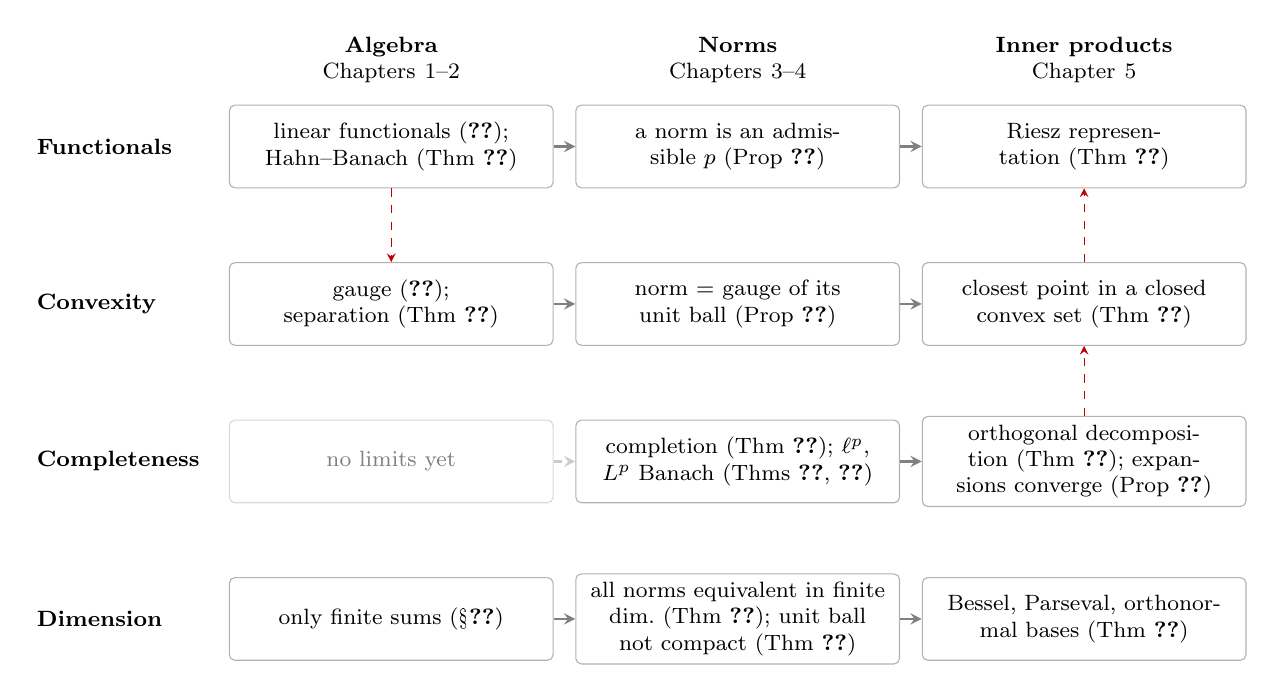
\begin{tikzpicture}[>=stealth, x=1cm, y=1cm,
    box/.style={draw=gray!60, rounded corners=2pt, fill=white, text width=3.9cm, align=center, font=\footnotesize, inner sep=3pt, minimum height=1.05cm},
    lab/.style={font=\footnotesize\bfseries, text width=2.4cm, align=left},
    hd/.style={font=\footnotesize\bfseries, align=center, text width=3.9cm}]
    \node[hd] at (3.3,1.1) {Algebra\\ \normalfont Chapters 1--2};
    \node[hd] at (7.7,1.1) {Norms\\ \normalfont Chapters 3--4};
    \node[hd] at (12.1,1.1) {Inner products\\ \normalfont Chapter 5};
    % functionals
    \node[lab] at (0,0) {Functionals};
    \node[box] (f1) at (3.3,0) {linear functionals (\ref{sec:maps-convex});\\ Hahn--Banach (Thm~\ref{thm:hb})};
    \node[box] (f2) at (7.7,0) {a norm is an admissible $p$ (Prop~\ref{prop:norm-gauge})};
    \node[box] (f3) at (12.1,0) {Riesz representation (Thm~\ref{thm:riesz-rep})};
    % convexity
    \node[lab] at (0,-2.0) {Convexity};
    \node[box] (c1) at (3.3,-2.0) {gauge (\ref{sec:gauge});\\ separation (Thm~\ref{thm:separation})};
    \node[box] (c2) at (7.7,-2.0) {norm $=$ gauge of its unit ball (Prop~\ref{prop:norm-gauge})};
    \node[box] (c3) at (12.1,-2.0) {closest point in a closed convex set (Thm~\ref{thm:projection})};
    % completeness
    \node[lab] at (0,-4.0) {Completeness};
    \node[box, draw=gray!30, text=gray] (k1) at (3.3,-4.0) {no limits yet};
    \node[box] (k2) at (7.7,-4.0) {completion (Thm~\ref{thm:completion-normed}); $\ell^p$, $L^p$ Banach (Thms~\ref{thm:lp-complete}, \ref{thm:Lp-complete})};
    \node[box] (k3) at (12.1,-4.0) {orthogonal decomposition (Thm~\ref{thm:orth-decomp}); expansions converge (Prop~\ref{prop:expansion-converges})};
    % dimension
    \node[lab] at (0,-6.0) {Dimension};
    \node[box] (d1) at (3.3,-6.0) {only finite sums (\S\ref{subsec:span})};
    \node[box] (d2) at (7.7,-6.0) {all norms equivalent in finite dim.\ (Thm~\ref{prop:norms-equiv}); unit ball not compact (Thm~\ref{thm:ball-noncompact})};
    \node[box] (d3) at (12.1,-6.0) {Bessel, Parseval, orthonormal bases (Thm~\ref{thm:onbasis-equiv})};
    % arrows along threads
    \foreach \a/\b in {f1/f2, f2/f3, c1/c2, c2/c3, k2/k3, d1/d2, d2/d3} \draw[->, thick, gray] (\a) -- (\b);
    \draw[->, thick, gray!40, dashed] (k1) -- (k2);
    % meeting points
    \draw[->, red!75!black, dashed] (f1) -- (c1);
    \draw[->, red!75!black, dashed] (k3) -- (c3);
    \draw[->, red!75!black, dashed] (c3) -- (f3);
\end{tikzpicture}
\end{center}
Solid arrows follow a thread from one stage to the next; dashed red arrows mark where threads meet: the separation theorem (Hahn--Banach applied to a gauge), the projection theorem (convexity needing completeness), and the Riesz representation theorem (built on the orthogonal decomposition).

\newpage

% ============================================================================
% CHAPTER 1: LINEAR SPACES
% ============================================================================
% Lecture 1 (2026-09-01)

\chapter{Linear Spaces}

Functional analysis is, in short, infinite-dimensional linear algebra. In finite dimensions the basic operation is summation; in infinite dimensions it is integration, and passing from finite to infinite dimension introduces genuine differences that the course will emphasize. We begin with the purely algebraic notions, with no topology yet.

\section{Linear Spaces}\label{sec:lin-spaces}

\roadmark{Stage: algebra}{Threads: dimension. The vocabulary of the course; only finite sums exist (\S\ref{subsec:span}), and the quotient stands in for an orthogonal complement until \ref{sec:projection}.}

\subsection{Definition and Examples}

Throughout, $\mathbb{F}$ denotes the scalar field, which is always $\mathbb{R}$ or $\mathbb{C}$.

\begin{defbox}[Linear Space]\boxlabel{def:linear-space}
We say $X$ is a \textbf{linear space} (or \textbf{vector space}) over the field $\mathbb{F}$ ($= \mathbb{R}$ or $\mathbb{C}$) if there are two operations on $X$, an addition
\[
+ : X \times X \to X, \qquad (x, y) \mapsto x + y,
\]
and a scalar multiplication
\[
\cdot : \mathbb{F} \times X \to X, \qquad (k, x) \mapsto kx,
\]
together with a distinguished element $0 \in X$, satisfying:
\begin{enumerate}[label=(\arabic*)]
    \item $x + y = y + x$ for all $x, y \in X$ \hfill (commutativity)
    \item $(x + y) + z = x + (y + z)$ for all $x, y, z \in X$ \hfill (associativity)
    \item $x + 0 = x$ for all $x \in X$ \hfill (additive identity)
    \item for every $x \in X$ there is an element $-x \in X$ with $x + (-x) = 0$ \hfill (additive inverse)
    \item $k(ax) = (ka)x$ for all $k, a \in \mathbb{F}$, $x \in X$
    \item $k(x + y) = kx + ky$ for all $k \in \mathbb{F}$, $x, y \in X$
    \item $(a + b)x = ax + bx$ for all $a, b \in \mathbb{F}$, $x \in X$
    \item $1x = x$ for all $x \in X$.
\end{enumerate}
\laxref{Ch.~1, axioms for a linear space}
\end{defbox}

\begin{rembox}\label{rem:lin-spaces}
The two operations are \emph{closed}: adding two elements of $X$, or multiplying an element of $X$ by a scalar, produces an element of $X$. This is the content of writing $+ : X \times X \to X$ and $kx \in X$ for all $k \in \mathbb{F}$, and is the property that must be checked first when verifying that a given set is a linear space.
\end{rembox}

\begin{exbox}[$\mathbb{R}^n$]\boxlabel{ex:rn}
$\mathbb{R}^n$ is a linear space over $\mathbb{R}$ with componentwise addition and scalar multiplication. It is $n$-dimensional: it has a basis, and every vector is a finite linear combination of basis vectors.
\end{exbox}

\subsection{Linear Subspaces}

\begin{defbox}[Linear Subspace]\boxlabel{def:linear-subspace}
Let $X$ be a linear space and $Y \subset X$. We say $Y$ is a \textbf{(linear) subspace} of $X$ if
\begin{enumerate}[label=(\roman*)]
    \item $y_1 + y_2 \in Y$ for all $y_1, y_2 \in Y$, and
    \item $ky \in Y$ for all $y \in Y$, $k \in \mathbb{F}$.
\end{enumerate}
In other words, $Y$ is a subset of $X$ that is itself a linear space under the operations inherited from $X$.
\laxref{Ch.~1, definition of linear subspace}
\end{defbox}

\begin{propbox}[Subspaces Contain the Origin]\boxlabel{prop:subspaces-contain-origin}
Every linear subspace $Y$ of $X$ contains $0$.
\end{propbox}

\begin{proof}
A subspace is nonempty by convention. Take any $y \in Y$; then $0 = 0 \cdot y \in Y$ by (ii).
\end{proof}

\begin{rembox}\label{rem:lin-spaces-2}
Geometrically, in $\mathbb{R}^3$ the subspaces are the origin, lines through the origin, planes through the origin, and $\mathbb{R}^3$ itself. A plane not passing through the origin is \emph{not} a subspace.
\end{rembox}

\begin{notebox}[Notation]\label{note:notation}
The inclusion $Y \subset X$ allows equality; $X$ is a subspace of itself. Strict inclusion, when it matters, is written $Y \subsetneq X$.
\end{notebox}

\subsection{Sums and Direct Sums}

\begin{defbox}[Sum of Subsets]\boxlabel{def:sum-of-subsets}
Let $X$ be a linear space and $S, T \subset X$ be subsets (not necessarily subspaces). The \textbf{sum} of $S$ and $T$ is
\[
S + T = \{ s + t \mid s \in S,\ t \in T \}.
\]
\laxref{Ch.~1, sum of subsets}
\end{defbox}

\begin{propbox}[Sum of Subspaces]\boxlabel{prop:sum}
If $S$ and $T$ are linear subspaces of $X$, then $S + T$ is a linear subspace of $X$.
\laxref{Ch.~1, Thm~1(ii)}
\end{propbox}

\begin{proof}
Let $s_1 + t_1, s_2 + t_2 \in S + T$ with $s_i \in S$, $t_i \in T$, and $k \in \mathbb{F}$. Then
\[
(s_1 + t_1) + (s_2 + t_2) = (s_1 + s_2) + (t_1 + t_2) \in S + T, \qquad k(s_1 + t_1) = ks_1 + kt_1 \in S + T,
\]
since $s_1 + s_2, ks_1 \in S$ and $t_1 + t_2, kt_1 \in T$.
\end{proof}

\begin{defbox}[Direct Sum]\boxlabel{def:direct-sum}
Let $X, Y$ be linear spaces over the same field. The \textbf{direct sum} of $X$ and $Y$, written $X \oplus Y$, is
\[
X \oplus Y = \{ (x, y) \mid x \in X,\ y \in Y \},
\]
with componentwise operations $(x_1, y_1) + (x_2, y_2) = (x_1 + x_2, y_1 + y_2)$ and $k(x, y) = (kx, ky)$.
\laxref{Ch.~1, direct sum}
\end{defbox}

\begin{exbox}[{{$\mathbb{R} \oplus \mathbb{R}^2 = \mathbb{R}^3$}}]\boxlabel{ex:r-oplus-r2-r3}
An element of $\mathbb{R} \oplus \mathbb{R}^2$ is a pair $(a, (b, c))$ with $a \in \mathbb{R}$ and $(b, c) \in \mathbb{R}^2$; identifying it with $(a, b, c)$ gives $\mathbb{R} \oplus \mathbb{R}^2 = \mathbb{R}^3$.
\end{exbox}

\begin{rembox}[Direct Sum vs.\ Sum; Comparison with Axler]\label{rem:direct-sum-vs-sum-comparison-axler}
The direct sum $X \oplus Y$ is a set of \emph{pairs}; it is what other texts call the (external) direct sum or the product $X \times Y$. It is defined for any two linear spaces, which need not sit inside a common ambient space. By contrast, $S + T$ is a set of \emph{vectors} in a fixed ambient space $X$.

This differs from the definition in Axler, where the direct sum $U_1 \oplus U_2$ is an \emph{internal} notion: it is the sum $U_1 + U_2$ of two subspaces of a common space, with the extra requirement that every element decomposes uniquely as $u_1 + u_2$. The convention here follows Lax. When the two internal summands are subspaces of a common $X$ with $U_1 \cap U_2 = \{0\}$, the two notions agree up to the isomorphism $(u_1, u_2) \mapsto u_1 + u_2$ (Proposition~\ref{prop:internal-external} below), but the course uses the external definition throughout.
\end{rembox}

\begin{propbox}[Internal and External Direct Sums]\boxlabel{prop:internal-external}
Let $U$ and $V$ be linear subspaces of a linear space $X$, and define
\[
\Phi : U \oplus V \to U + V, \qquad \Phi(u, v) = u + v .
\]
Then $\Phi$ is linear and onto, and the following are equivalent:
\begin{enumerate}[label=(\roman*)]
    \item $\Phi$ is an isomorphism;
    \item $U \cap V = \{0\}$;
    \item every element of $U + V$ can be written as $u + v$ with $u \in U$, $v \in V$ in exactly one way.
\end{enumerate}
\end{propbox}

\begin{proof}
(Not covered in lecture.) $\Phi$ is linear because the operations on $U \oplus V$ are componentwise, and onto by the definition of $U + V$. So (i) says that $\Phi$ is one-to-one, and (iii) says the same thing, since $\Phi(u,v) = \Phi(u',v')$ means $u + v = u' + v'$. It remains to show that $\Phi$ is one-to-one iff $U \cap V = \{0\}$. If $U \cap V = \{0\}$ and $u + v = u' + v'$, then $u - u' = v' - v$ lies in $U \cap V$, so $u = u'$ and $v = v'$. Conversely, if $0 \neq w \in U \cap V$, then $\Phi(w, -w) = 0 = \Phi(0, 0)$ although $(w, -w) \neq (0, 0)$.
\end{proof}

\subsection{Linear Span}\label{subsec:span}

\begin{defbox}[Linear Span]\boxlabel{def:linear-span}
Let $X$ be a linear space and $S \subset X$ a subset. The \textbf{linear span} of $S$, written $\operatorname{span}\{S\}$, is the smallest linear subspace of $X$ containing $S$.
\laxref{Ch.~1, definition of linear span}
\end{defbox}

\begin{propbox}[The Smallest Subspace Exists]\boxlabel{prop:the-smallest-subspace-exists}
Let $S \subset X$. The intersection of any family of linear subspaces of $X$ is a linear subspace, and
\[
\operatorname{span}\{S\} = \bigcap \{ W : W \text{ a linear subspace of } X,\ S \subset W \}.
\]
In particular the smallest subspace containing $S$ exists, so the definition of span is meaningful.
\laxref{Ch.~1, Thm~2(i)}
\end{propbox}

\begin{proof}
Let $\{W_i\}_{i \in I}$ be subspaces and $W = \bigcap_i W_i$. If $x, y \in W$ and $k \in \mathbb{F}$, then $x + y \in W_i$ and $kx \in W_i$ for every $i$, so $x + y, kx \in W$; hence $W$ is a subspace. (For $I = \varnothing$ the intersection is $X$, also a subspace.)

Now let $W_S$ be the intersection of all subspaces containing $S$; the family is nonempty since $X$ belongs to it. Then $W_S$ is a subspace, $S \subset W_S$, and $W_S \subset W$ for every subspace $W \supset S$. So $W_S$ is the smallest subspace containing $S$, i.e.\ $W_S = \operatorname{span}\{S\}$.
\end{proof}

\begin{exbox}[Span of a Single Vector]\boxlabel{ex:span-single-vector}
Let $s_0 \in \mathbb{R}^2$ be a nonzero vector. Then
\[
\operatorname{span}\{s_0\} = \{ a s_0 \mid a \in \mathbb{R} \},
\]
the line through the origin in the direction of $s_0$: for $a > 0$ one stretches in the positive direction, for $a < 0$ in the negative direction.

\begin{center}
\begin{tikzpicture}[scale=1.1, >=stealth]
    \draw[->] (-1.8,0) -- (2.6,0);
    \draw[->] (0,-1.2) -- (0,1.8);
    \draw[dashed] (-1.6,-1.07) -- (2.4,1.6) node[right] {$\operatorname{span}\{s_0\}$};
    \draw[->, thick] (0,0) -- (1.2,0.8) node[pos=0.6, above left] {$s_0$};
    \fill (1.8,1.2) circle (1.2pt) node[below right, font=\footnotesize, yshift=-2pt] {$a s_0$, $a>1$};
    \fill (-0.9,-0.6) circle (1.2pt) node[left, font=\footnotesize, xshift=-2pt] {$a s_0$, $a<0$};
\end{tikzpicture}
\end{center}
\end{exbox}

\begin{propbox}[Span as Finite Linear Combinations]\boxlabel{prop:span-as-finite-linear}
For any subset $S$ of a linear space $X$,
\[
\operatorname{span}\{S\} = \Bigl\{ \sum_{i=1}^{k} a_i s_i \;\Big|\; k \geq 1,\ a_i \in \mathbb{F},\ s_i \in S \Bigr\},
\]
the set of all \emph{finite} linear combinations of elements of $S$ (with $\operatorname{span}\{\varnothing\} = \{0\}$).
\laxref{Ch.~1, Thm~2(ii)}
\end{propbox}

\begin{proof}
Let $L$ denote the set of finite linear combinations of elements of $S$. Then $L$ is a subspace: the sum of two finite linear combinations is again a finite linear combination (concatenate the two sums), and a scalar multiple of a finite linear combination is a finite linear combination (multiply each coefficient). Also $S \subset L$ (take $k = 1$, $a_1 = 1$). So $\operatorname{span}\{S\} \subset L$ by minimality.

Conversely, any subspace containing $S$ contains every sum $\sum_{i=1}^k a_i s_i$ by closure under addition and scalar multiplication applied finitely many times, so $L \subset \operatorname{span}\{S\}$.
\end{proof}

\begin{rembox}[Why Only Finite Sums]\label{rem:why-only-finite-sums}
The sums in the span are finite. We do not, at this point, know how to form an infinite sum of vectors: an infinite sum requires taking a limit, and a linear space carries no notion of limit. Adding two vectors is part of the structure; passing to infinitely many is not, and must be separately justified once a topology is available. Finite sums are also already enough to produce a subspace, as the proof shows.
\end{rembox}

\subsection{Quotient Spaces}\label{subsec:quotient}

\begin{defbox}[Equivalence mod $Y$]\boxlabel{def:equivalence-mod}
Let $X$ be a linear space and $Y$ a linear subspace of $X$. We say $x_1, x_2 \in X$ are \textbf{equivalent mod $Y$}, written
\[
x_1 \equiv x_2 \pmod{Y},
\]
if $x_1 - x_2 \in Y$.
\laxref{Ch.~1, equivalence mod $Y$}
\end{defbox}

\begin{defbox}[Equivalence Class and Quotient Space]\boxlabel{def:equivalence-class-and-quotient}
For $x_0 \in X$, the \textbf{equivalence class} of $x_0$ is
\[
[x_0] = \{ x \in X \mid x - x_0 \in Y \} = x_0 + Y.
\]
The \textbf{quotient space} $X / Y$ ($X$ mod $Y$) is the set of all equivalence classes:
\[
X / Y = \{ [x] \mid x \in X \}.
\]
\laxref{Ch.~1, quotient space}
\end{defbox}

\begin{exbox}[Geometry of Equivalence Classes]\boxlabel{ex:geometry-equivalence-classes}
Let $X = \mathbb{R}^2$ and let $Y$ be a line through the origin. If $x_0 = 0$ then $[x_0] = Y$. For general $x_0$, the class $[x_0] = x_0 + Y$ is the line \emph{parallel} to $Y$ passing through the tip of the vector $x_0$: any other point $x$ on this line, dragged back by $-x_0$, lands on $Y$, i.e.\ $x - x_0 \in Y$. The equivalence classes are therefore the parallel translates of $Y$. They are not subspaces (they do not contain the origin unless equal to $Y$); the quotient $X / Y$ is the collection of all these parallel lines.

\begin{center}
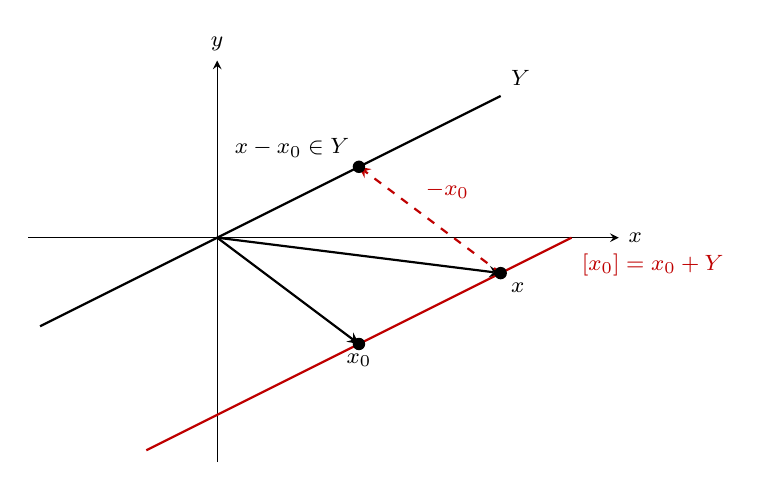
\begin{tikzpicture}[scale=1.5, >=stealth]
    \draw[->] (-1.6,0) -- (3.4,0) node[right] {$x$};
    \draw[->] (0,-1.9) -- (0,1.5) node[above] {$y$};
    \draw[thick] (-1.5,-0.75) -- (2.4,1.2) node[above right] {$Y$};
    \draw[thick, red!75!black] (-0.6,-1.8) -- (3.0,0.0) node[below right, yshift=-2pt] {$[x_0] = x_0 + Y$};
    % the vectors x_0 and x
    \draw[->, thick] (0,0) -- (1.2,-0.9) node[below] {$x_0$};
    \draw[->, thick] (0,0) -- (2.4,-0.3) node[below right] {$x$};
    % dragging x back to Y by -x_0
    \draw[->, dashed, thick, red!75!black] (2.4,-0.3) -- (1.2,0.6) node[pos=0.6, above right, font=\footnotesize] {$-x_0$};
    \fill (1.2,0.6) circle (1.5pt) node[above left, font=\footnotesize] {$x - x_0 \in Y$};
    \fill (1.2,-0.9) circle (1.5pt);
    \fill (2.4,-0.3) circle (1.5pt);
\end{tikzpicture}
\end{center}
\end{exbox}

\begin{propbox}[$X/Y$ is a Linear Space]\boxlabel{prop:quotient}
The operations
\[
[x_1] + [x_2] = [x_1 + x_2], \qquad k[x] = [kx]
\]
are well defined on $X / Y$ and make $X / Y$ a linear space over $\mathbb{F}$, with zero element $[0] = Y$.
\laxref{Ch.~1, quotient space}
\end{propbox}

\begin{proof}
(HW1, Problem 1.) \textbf{Well-definedness.} Suppose $[x_1] = [x_1']$ and $[x_2] = [x_2']$, i.e.\ $x_1 - x_1' \in Y$ and $x_2 - x_2' \in Y$. Then
\[
(x_1 + x_2) - (x_1' + x_2') = (x_1 - x_1') + (x_2 - x_2') \in Y, \qquad kx_1 - kx_1' = k(x_1 - x_1') \in Y,
\]
since $Y$ is a subspace. Hence $[x_1 + x_2] = [x_1' + x_2']$ and $[kx_1] = [kx_1']$: the operations do not depend on the representatives.

\textbf{The axioms.} Let $[x], [y], [z] \in X/Y$ and $a, k \in \mathbb{F}$. In each line the outer equalities are the definitions of the operations on $X/Y$, and the middle equality is the corresponding axiom of $X$.

\emph{Commutativity:} $[x] + [y] = [x + y] = [y + x] = [y] + [x]$.

\emph{Associativity:} $([x] + [y]) + [z] = [x + y] + [z] = [(x + y) + z] = [x + (y + z)] = [x] + [y + z] = [x] + ([y] + [z])$.

\emph{Additive identity:} $[0] = Y \in X/Y$, and $[x] + [0] = [x + 0] = [x] = [0 + x] = [0] + [x]$.

\emph{Additive inverse:} $[-x] \in X/Y$, and $[x] + [-x] = [x - x] = [0] = [-x + x] = [-x] + [x]$.

\emph{Compatibility of scalar multiplication:} $k(a[x]) = k[ax] = [k(ax)] = [(ka)x] = (ka)[x]$.

\emph{Distributivity over vector addition:} $k([x] + [y]) = k[x + y] = [k(x + y)] = [kx + ky] = [kx] + [ky] = k[x] + k[y]$.

\emph{Distributivity over scalar addition:} $(a + k)[x] = [(a + k)x] = [ax + kx] = [ax] + [kx] = a[x] + k[x]$.

\emph{Unit:} $1[x] = [1x] = [x]$.

Hence $X/Y$ is a linear space over $\mathbb{F}$ with zero element $[0] = Y$.
\end{proof}

\begin{rembox}\label{rem:lin-spaces-3}
The pattern of the verification is the same in every line: the outer equalities are the definitions of the operations on $X/Y$ and the middle equality is the corresponding axiom of $X$, e.g.\ $k([x_1]+[x_2]) = k[x_1+x_2] = [k(x_1+x_2)] = [kx_1+kx_2] = k[x_1]+k[x_2]$. The additive inverse is $-[x] = [-x]$.
\end{rembox}

\begin{rembox}[Quotients and Orthogonal Complements]\label{rem:quotients-orthogonal-complements}
In $\mathbb{R}^n$, one may think of $X / Y$ as playing the role of the orthogonal complement $Y^\perp$: each parallel translate $x_0 + Y$ meets $Y^\perp$ in exactly one point. But ``orthogonal'' requires an inner product, and a bare linear space has no such structure. The quotient space is the substitute that is available in full generality. Wu suggested in lecture that $(X/Y) \oplus Y \cong X$ ``in some sense''; this became HW1, and the precise statement needs no inner product at all --- only a subspace $W$ playing the role of $Y^\perp$. The tools are extracted below.
\end{rembox}

\subsection{Complements and the Isomorphism $X \cong X/Y \oplus Y$}\label{subsec:complements}

Throughout this subsection $Y$ is a fixed linear subspace of $X$. The material is from HW1.

\begin{defbox}[Complement]\boxlabel{def:complement}
A linear subspace $W \subset X$ is a \textbf{complement} of $Y$ if
\[
W \cap Y = \{0\} \qquad \text{and} \qquad W + Y = X.
\]
\end{defbox}

\begin{lembox}[One-Step Enlargement]\boxlabel{lem:enlarge}
Let $W \subset X$ be a linear subspace with $W \cap Y = \{0\}$, and let $x_0 \in X$ with $x_0 \notin W + Y$. Then $W' = W + \operatorname{span}\{x_0\}$ is a linear subspace with $W' \cap Y = \{0\}$ and $W \subsetneq W'$.
\end{lembox}

\begin{proof}
$W'$ is a subspace as a sum of subspaces (Proposition~\ref{prop:sum}).

\emph{Strictness.} $x_0 \in W'$. If $x_0 \in W$ then $x_0 = x_0 + 0 \in W + Y$, contradicting the hypothesis; so $x_0 \in W' \setminus W$.

\emph{Intersection.} Let $w' \in W' \cap Y$, and write $w' = a x_0 + w$ with $a \in \mathbb{F}$, $w \in W$; put $y = w' \in Y$, so $a x_0 + w = y$. If $a \neq 0$, dividing by $a$ and rearranging gives
\[
x_0 = \frac{y}{a} - \frac{w}{a} \in Y + W,
\]
contradicting $x_0 \notin W + Y$. Hence $a = 0$, so $w' = w \in W \cap Y = \{0\}$. Thus $W' \cap Y = \{0\}$.
\end{proof}

\begin{propbox}[Every Subspace Has a Complement]\boxlabel{prop:complement}
For every linear subspace $Y \subset X$ there exists a complement $W$ of $Y$.
\end{propbox}

\begin{proof}
Let $P = \{ W \subset X \text{ a linear subspace} : W \cap Y = \{0\} \}$, partially ordered by inclusion; $\{0\} \in P$. Chains in $P$ have upper bounds: the union of a chain of subspaces is a subspace (the argument in the proof of Theorem~\ref{thm:hb}), and it meets $Y$ only in $0$ since each member does. By Zorn's lemma (Theorem~\ref{thm:zorn}) $P$ has a maximal element $W$. If $W + Y \neq X$, pick $x_0 \in X \setminus (W + Y)$; Lemma~\ref{lem:enlarge} gives a strictly larger element of $P$, contradicting maximality. Hence $W + Y = X$, and $W$ is a complement.
\end{proof}

\begin{rembox}\label{rem:lin-spaces-4}
When $\dim X < \infty$ Zorn's lemma is unnecessary: starting from $W = \{0\}$ and applying Lemma~\ref{lem:enlarge} repeatedly, $\dim W$ increases by one each time and the process stops after at most $\dim X - \dim Y$ steps.
\end{rembox}

\begin{propbox}[When the Complement is Unique]\boxlabel{prop:complement-unique}
A linear subspace $Y$ of $X$ has exactly one complement if and only if $Y = \{0\}$ or $Y = X$.
\end{propbox}

\begin{proof}
If $Y = \{0\}$, a complement $W$ satisfies $W = W + \{0\} = X$; if $Y = X$, it satisfies $W = W \cap X = \{0\}$. In both cases the complement is unique.

Suppose $\{0\} \neq Y \neq X$, and let $W$ be a complement (Proposition~\ref{prop:complement}). Then $W \neq \{0\}$, since $W + Y = X \neq Y$. Choose $0 \neq y_0 \in Y$ and $0 \neq w_0 \in W$. Applying Proposition~\ref{prop:complement} inside the linear space $W$, the subspace $\operatorname{span}\{w_0\}$ has a complement $W_1$ in $W$: $\operatorname{span}\{w_0\} \cap W_1 = \{0\}$ and $\operatorname{span}\{w_0\} + W_1 = W$. Put
\[
W' = \operatorname{span}\{w_0 + y_0\} + W_1 .
\]
\emph{$W' \cap Y = \{0\}$.} If $a(w_0 + y_0) + w_1 \in Y$ with $a \in \mathbb{F}$, $w_1 \in W_1$, then subtracting $a y_0 \in Y$ gives $a w_0 + w_1 \in Y \cap W = \{0\}$; so $a w_0 = -w_1 \in \operatorname{span}\{w_0\} \cap W_1 = \{0\}$, whence $a = 0$ and $w_1 = 0$.

\emph{$W' + Y = X$.} $w_0 = (w_0 + y_0) - y_0 \in W' + Y$ and $W_1 \subset W'$, so $W = \operatorname{span}\{w_0\} + W_1 \subset W' + Y$, and $X = W + Y \subset W' + Y$.

\emph{$W' \neq W$.} $w_0 + y_0 \in W'$; if it were in $W$, then $y_0 = (w_0 + y_0) - w_0 \in W \cap Y = \{0\}$, a contradiction.

So $W'$ is a second complement of $Y$. (Not covered in lecture.)
\end{proof}

\begin{exbox}[Complements of a Line in the Plane]\boxlabel{ex:complements-line-plane}
In $\mathbb{R}^2$ with $Y$ the $x$-axis, every line through the origin other than $Y$ is a complement of $Y$.
\end{exbox}

\begin{lembox}[Unique Decomposition]\boxlabel{lem:unique-decomp}
Let $W$ be a complement of $Y$. Then every $x \in X$ can be written as $x = w + y$ with $w \in W$, $y \in Y$, and this representation is unique.
\end{lembox}

\begin{proof}
Existence is $X = W + Y$. If $w_1 + y_1 = w_2 + y_2$, then $w_1 - w_2 = y_2 - y_1$ lies in both $W$ and $Y$, hence in $W \cap Y = \{0\}$; so $w_1 = w_2$ and $y_1 = y_2$.
\end{proof}

This is the implication (ii)$\Rightarrow$(iii) of Proposition~\ref{prop:internal-external}, applied to $W$ and $Y$.

\begin{thmbox}[$X \cong X/Y \oplus Y$]\boxlabel{thm:quotient-iso}
Let $W$ be a complement of $Y$. The map
\[
M : X \to X/Y \oplus Y, \qquad M(x) = ([w], y) \quad \text{where } x = w + y,\ w \in W,\ y \in Y,
\]
is an isomorphism. Consequently $X/Y \oplus Y \cong X$, with inverse $M^{-1}([x], y) = w + y$, where $w$ is the unique element of $W$ with $[w] = [x]$.
\end{thmbox}

\begin{proof}
$M$ is well defined by Lemma~\ref{lem:unique-decomp}.

\emph{Linearity.} If $x_i = w_i + y_i$ and $a, b \in \mathbb{F}$, then $a x_1 + b x_2 = (a w_1 + b w_2) + (a y_1 + b y_2)$ with the two summands in $W$ and $Y$ respectively; by uniqueness this \emph{is} the decomposition of $a x_1 + b x_2$, so
\[
M(a x_1 + b x_2) = \bigl([a w_1 + b w_2],\, a y_1 + b y_2\bigr) = a([w_1], y_1) + b([w_2], y_2) = a M(x_1) + b M(x_2),
\]
using the operations on $X/Y$ (Proposition~\ref{prop:quotient}) and the componentwise operations on the direct sum.

\emph{Surjectivity.} Given $([x], y)$, decompose $x = w + y'$. Then $x - w = y' \in Y$, so $[x] = [w]$, and $M(w + y) = ([w], y) = ([x], y)$.

\emph{Injectivity.} If $M(x_1) = M(x_2)$ with $x_i = w_i + y_i$, then $y_1 = y_2$ and $[w_1] = [w_2]$, i.e.\ $w_1 - w_2 \in Y$; also $w_1 - w_2 \in W$, so $w_1 - w_2 \in W \cap Y = \{0\}$. Hence $x_1 = x_2$.

$M$ is a linear bijection, hence an isomorphism, and $M^{-1}$ is an isomorphism by Lemma~\ref{lem:inverse-iso}. The formula for $M^{-1}$ is read off from the surjectivity computation.
\end{proof}

\begin{corbox}[A Complement is a Model of the Quotient]\boxlabel{cor:complement-quotient}
If $W$ is a complement of $Y$, then the restricted quotient map $W \to X/Y$, $w \mapsto [w]$, is an isomorphism. In particular all complements of $Y$ are isomorphic to one another.
\end{corbox}

\begin{proof}
Linearity is inherited from the quotient map. Injectivity and surjectivity are exactly the two computations in the proof of Theorem~\ref{thm:quotient-iso}: $[w_1] = [w_2]$ forces $w_1 - w_2 \in W \cap Y = \{0\}$, and every class $[x]$ equals $[w]$ for the $W$-component $w$ of $x$.
\end{proof}

\begin{rembox}[The Isomorphism is Not Canonical]\label{rem:isomorphism-not-canonical}
$M$ depends on the choice of complement $W$. The quotient $X/Y$ itself is canonical --- it is built from $X$ and $Y$ alone --- but identifying it with a subspace of $X$ requires choosing $W$, and different choices give different embeddings. This is the precise content of ``$X/Y$ is like a complement of $Y$'': it is isomorphic to every complement, and equal to none.
\end{rembox}

\begin{corbox}[Orthogonal Complement (inner products; later)]\boxlabel{cor:orth}
Let $X$ carry an inner product $\langle \cdot, \cdot \rangle$ and let $Y^\perp = \{ z \in X : \langle z, y \rangle = 0 \ \forall y \in Y \}$. If $X = Y + Y^\perp$, then $Y^\perp$ is a complement of $Y$, so $X/Y \cong Y^\perp$ via $z \mapsto [z]$ and $X \cong X/Y \oplus Y$.
\end{corbox}

\begin{proof}
If $z \in Y \cap Y^\perp$ then $\langle z, z \rangle = 0$, so $z = 0$ by positive-definiteness of the inner product (to be introduced later). With $X = Y + Y^\perp$ assumed, $Y^\perp$ is a complement; apply Corollary~\ref{cor:complement-quotient} and Theorem~\ref{thm:quotient-iso}.
\end{proof}

\begin{rembox}\label{rem:lin-spaces-5}
The hypothesis $X = Y + Y^\perp$ holds automatically in finite dimensions, and in infinite dimensions it holds when $X$ is complete and $Y$ is closed (the orthogonal decomposition theorem, Theorem~\ref{thm:orth-decomp}). It can fail for a general subspace: in $\ell^2$ with the inner product of Chapter~5, the finitely supported sequences form a subspace $Y$ with $Y^\perp = \{0\}$, since $(z, e_i) = z_i$, so $Y + Y^\perp = Y \neq \ell^2$. Then $Y^\perp$ is \emph{not} a complement --- although by Proposition~\ref{prop:complement} some other complement always exists. This is why the orthogonal version is only ``roughly'' true, while the algebraic version (Theorem~\ref{thm:quotient-iso}) is unconditional.
\end{rembox}

% ============================================================================
% SECTION 2: LINEAR MAPS, CONVEXITY, AND LINEAR FUNCTIONALS
% ============================================================================
\section{Linear Maps, Convexity, and Linear Functionals}\label{sec:maps-convex}

\roadmark{Stage: algebra}{Threads: functionals, convexity. Introduces the two objects that Chapter 2 connects.}

\subsection{Linear Maps and Isomorphisms}

\begin{defbox}[Linear Map]\boxlabel{def:linear-map}
Let $X, Y$ be linear spaces over the same field $\mathbb{F}$. A map $M : X \to Y$ is called a \textbf{linear map} if
\[
M(a_1 x_1 + a_2 x_2) = a_1 M(x_1) + a_2 M(x_2) \qquad \text{for all } x_1, x_2 \in X,\ a_1, a_2 \in \mathbb{F}.
\]
That is, $M$ preserves the linear operations.
\laxref{Ch.~1, definition of linear map}
\end{defbox}

\begin{defbox}[Isomorphism]\boxlabel{def:isomorphism}
A map $M : X \to Y$ is an \textbf{isomorphism} (or \textbf{linear isomorphism}) if $M$ is linear, one-to-one, and onto.
\laxref{Ch.~1, definition of isomorphism; Remark~2}
\end{defbox}

\begin{rembox}\label{rem:maps-convex}
If there is an isomorphism $X \to Y$, the two linear spaces can be regarded as identical as far as the linear structure is concerned: every statement about linear combinations in $X$ transfers to $Y$ and back.
\end{rembox}

\begin{lembox}[Inverse of an Isomorphism]\boxlabel{lem:inverse-iso}
Let $A, B$ be linear spaces over the same field and $\varphi : A \to B$ an isomorphism. Then $\varphi^{-1} : B \to A$ is an isomorphism.
\end{lembox}

\begin{proof}
$\varphi^{-1}$ exists and is bijective since $\varphi$ is. For linearity, let $u_1, u_2 \in B$, $a, b \in \mathbb{F}$, and set $v = a\,\varphi^{-1}(u_1) + b\,\varphi^{-1}(u_2) \in A$. By linearity of $\varphi$ and $\varphi \circ \varphi^{-1} = \mathrm{id}_B$,
\[
\varphi(v) = a\,\varphi(\varphi^{-1}(u_1)) + b\,\varphi(\varphi^{-1}(u_2)) = a u_1 + b u_2,
\]
and applying $\varphi^{-1}$ gives $\varphi^{-1}(a u_1 + b u_2) = v$, which is linearity of $\varphi^{-1}$. (From HW1.)
\end{proof}

\subsection{Convex Sets}

\begin{defbox}[Convex Set]\boxlabel{def:convex-set}
Let $X$ be a linear space over $\mathbb{R}$. A set $K \subset X$ is called \textbf{convex} if for all $x_1, x_2 \in K$ and all $a \in [0, 1]$,
\[
a x_1 + (1 - a) x_2 \in K.
\]
\laxref{Ch.~1, definition of convex set}
\end{defbox}

\begin{rembox}\label{rem:maps-convex-2}
As $a$ runs over $[0, 1]$, the point $a x_1 + (1 - a) x_2$ runs over the line segment from $x_2$ (at $a = 0$) to $x_1$ (at $a = 1$). So $K$ is convex if and only if it contains the segment joining any two of its points. Values $a > 1$ or $a < 0$ would leave the segment, continuing beyond $x_1$ or beyond $x_2$ respectively; these are excluded.
\end{rembox}

\begin{defbox}[Convex Hull]\boxlabel{def:convex-hull}
The \textbf{convex hull} of a subset $S \subset X$ is the smallest convex set containing $S$.
\laxref{Ch.~1, definition of convex hull}
\end{defbox}

\begin{propbox}[The Smallest Convex Set Exists]\boxlabel{prop:the-smallest-convex-set}
The intersection of any family of convex sets is convex, and the convex hull of $S$ is the intersection of all convex subsets of $X$ containing $S$.
\laxref{Ch.~1, Thm~5(vi) and Thm~6(i)}
\end{propbox}

\begin{proof}
Let $\{K_i\}$ be convex and $K = \bigcap_i K_i$. If $x_1, x_2 \in K$ and $a \in [0,1]$ then $a x_1 + (1-a) x_2 \in K_i$ for every $i$, so it lies in $K$. The family of convex sets containing $S$ is nonempty ($X$ is convex), and its intersection is convex, contains $S$, and is contained in every convex set containing $S$; it is therefore the convex hull.
\end{proof}

\begin{exbox}[Convex Hull of a Star]\boxlabel{ex:convex-hull-star}
Let $S \subset \mathbb{R}^2$ be a four-pointed star (the boundary of the region obtained from a square by pushing the midpoints of its edges inward). The convex hull of $S$ is the filled square with the star's four tips as vertices. Indeed, taking any two tips, the whole segment between them must be included; taking any point of $S$ and any point already included, the segment between them must be included; iterating fills the square, which is itself convex.

\begin{center}
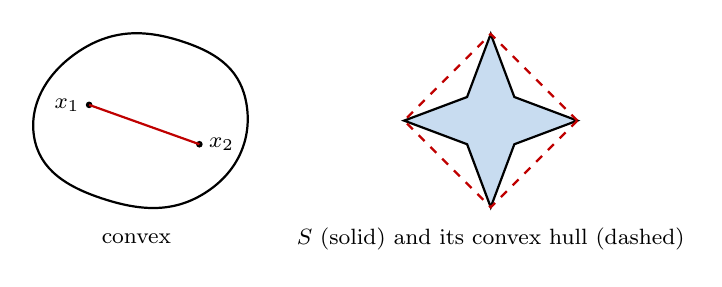
\begin{tikzpicture}[scale=1.0, >=stealth]
    % convex blob
    \begin{scope}
        \draw[thick] plot[smooth cycle, tension=0.8] coordinates {(-1.3,-0.2) (-0.7,0.9) (0.6,1.0) (1.4,0.2) (0.9,-0.9) (-0.4,-1.0)};
        \fill (-0.6,0.2) circle (1.2pt) node[left, font=\footnotesize] {$x_1$};
        \fill (0.8,-0.3) circle (1.2pt) node[right, font=\footnotesize] {$x_2$};
        \draw[thick, red!75!black] (-0.6,0.2) -- (0.8,-0.3);
        \node[font=\footnotesize] at (0,-1.5) {convex};
    \end{scope}
    % star and its hull
    \begin{scope}[xshift=4.5cm]
        \fill[axlerblue] (1.1,0) -- (0.3,0.3) -- (0,1.1) -- (-0.3,0.3) -- (-1.1,0) -- (-0.3,-0.3) -- (0,-1.1) -- (0.3,-0.3) -- cycle;
        \draw[thick] (1.1,0) -- (0.3,0.3) -- (0,1.1) -- (-0.3,0.3) -- (-1.1,0) -- (-0.3,-0.3) -- (0,-1.1) -- (0.3,-0.3) -- cycle;
        \draw[dashed, thick, red!75!black] (1.1,0) -- (0,1.1) -- (-1.1,0) -- (0,-1.1) -- cycle;
        \node[font=\footnotesize] at (0,-1.5) {$S$ (solid) and its convex hull (dashed)};
    \end{scope}
\end{tikzpicture}
\end{center}
\end{exbox}

\subsection{Linear Functionals}

\begin{defbox}[Linear Functional]\boxlabel{def:linear-functional}
Let $X$ be a linear space over $\mathbb{F}$. A linear map $\ell : X \to \mathbb{F}$ is called a \textbf{linear functional} on $X$.
\laxref{\S3.1, definition of linear functional}
\end{defbox}

Here $\mathbb{F}$ is regarded as a one-dimensional linear space over itself, so a linear functional is simply a linear map into the scalars.

\begin{exbox}[Linear Functionals on $\mathbb{R}^n$]\boxlabel{ex:functionals-rn}
Let $a = (a_1, \ldots, a_n) \in \mathbb{R}^n$. Then
\[
\ell(x) = a_1 x_1 + \cdots + a_n x_n = a \cdot x, \qquad x = (x_1, \ldots, x_n),
\]
is a linear functional on $\mathbb{R}^n$. Conversely, \emph{every} linear functional on $\mathbb{R}^n$ has this form: writing $x = \sum_{i=1}^n x_i e_i$ in the standard basis and setting $a_i = \ell(e_i)$, linearity gives
\[
\ell(x) = \sum_{i=1}^n x_i\, \ell(e_i) = \sum_{i=1}^n a_i x_i = a \cdot x.
\]
So on $\mathbb{R}^n$ a linear functional is determined by its $n$ values on a basis, and there is nothing else to say.
\end{exbox}

\begin{rembox}[Why Abstract Tools are Needed]\label{rem:why-abstract-tools-needed}
On $\mathbb{R}^n$ linear functionals are completely explicit because a basis is available. On a general linear space $X$ there is no such description: we do not even know the dimension, and there is no canonical way to write down a linear functional. The Hahn--Banach theorem below is the basic tool for \emph{constructing} linear functionals on a general $X$.
\end{rembox}

% ============================================================================
% CHAPTER 2: THE HAHN-BANACH THEOREM
% ============================================================================

\chapter{The Hahn--Banach Theorem}

On $\mathbb{R}^n$ every linear functional is $x \mapsto a \cdot x$, and there is nothing to construct. On a general linear space there is no basis to hand and no formula for a single nonzero functional; the Hahn--Banach theorem is the device that produces them. Everything in this chapter is still pure algebra and convexity --- there is no norm and no limit anywhere --- and the only notion resembling analysis is the algebraic interior point of \ref{sec:gauge}. The chapter states the extension theorem (\ref{sec:hb-statement}) and proves it by a one-step extension followed by Zorn's lemma (\ref{sec:hb-proof}); translates between convex sets and positive homogeneous subadditive functions through the gauge (\ref{sec:gauge}); combines the two in the hyperplane separation theorem (\ref{sec:separation}); and extends the theorem to complex scalars (\ref{sec:hb-complex}).

\section{Statement and Motivation}\label{sec:hb-statement}

\roadmark{Stage: algebra}{Thread: functionals. The extension problem, with $\ell$ dominated by a positive homogeneous subadditive $p$.}

\subsection{Positive Homogeneous Subadditive Functions}

\begin{defbox}[Positive Homogeneous; Subadditive]\boxlabel{def:positive-homogeneous-subadditive}
Let $X$ be a linear space over $\mathbb{R}$. A function $p : X \to \mathbb{R}$ is
\begin{enumerate}[label=(\arabic*)]
    \item \textbf{positive homogeneous} if $p(ax) = a\,p(x)$ for all $a \geq 0$ and all $x \in X$;
    \item \textbf{subadditive} if $p(x + y) \leq p(x) + p(y)$ for all $x, y \in X$.
\end{enumerate}
\laxref{\S3.1, conditions (1)--(2) of Thm~1}
\end{defbox}

\begin{rembox}\label{rem:hb-statement}
Positive homogeneity only involves scalars $a \geq 0$: multiplying $x$ by a non-negative real number pulls that number out of $p$. Nothing is said about negative scalars, and $p$ is \emph{not} required to be non-negative. (For a norm, non-negativity is part of the definition; here it is not assumed.)
\end{rembox}

\begin{lembox}[{{$p(0) = 0$}}]\boxlabel{lem:p-zero}
If $p : X \to \mathbb{R}$ is positive homogeneous, then $p(0) = 0$.
\end{lembox}

\begin{proof}
Take any $x \in X$. Positive homogeneity with $a = 0$ (allowed, since $a \ge 0$) gives
\[
p(0) = p(0 \cdot x) = 0 \cdot p(x) = 0. \qedhere
\]
\end{proof}

\begin{rembox}[Comparison with Lax]\label{rem:comparison-lax}
Lax requires $p(ax) = a\,p(x)$ only for $a > 0$. The two definitions agree: for $a > 0$ alone, $p(0) = p(2 \cdot 0) = 2p(0)$ gives $p(0) = 0$, which is the case $a = 0$.
\end{rembox}

Subadditivity is not needed. Note also that the argument uses $p(x) \in \mathbb{R}$: the product $0 \cdot p(x)$ is $0$ only because $p(x)$ is a finite number, which is why the gauge later must first be shown finite.

\begin{exbox}[Three Examples on $\mathbb{R}^n$]\boxlabel{ex:three-p}
On $X = \mathbb{R}^n$, the following are positive homogeneous and subadditive:
\begin{enumerate}[label=(\alph*)]
    \item $p_1(x) = \Bigl(\sum_{i=1}^n x_i^2\Bigr)^{1/2} = \|x\|$, the Euclidean length. For $a \geq 0$,
    \[
    p_1(ax) = \Bigl(\sum_{i=1}^n a^2 x_i^2\Bigr)^{1/2} = a\,\|x\|,
    \]
    and $\|x + y\| \leq \|x\| + \|y\|$ is the triangle inequality.
    \item $p_2(x) = \max_{1 \leq i \leq n} |x_i|$. For $a \geq 0$, $\max_i |a x_i| = a \max_i |x_i|$; and $|x_i + y_i| \leq |x_i| + |y_i| \leq p_2(x) + p_2(y)$ for each $i$, so $p_2(x + y) \leq p_2(x) + p_2(y)$.
    \item $p_3(x) = |x_1| + \cdots + |x_n|$. For $a \geq 0$, $\sum_i |a x_i| = a \sum_i |x_i|$; and $\sum_i |x_i + y_i| \leq \sum_i (|x_i| + |y_i|) = p_3(x) + p_3(y)$.
\end{enumerate}
Each of these is in fact a norm, so a positive homogeneous subadditive function is ``like a norm.'' Norms will be introduced later; for now only these two properties are needed.
\end{exbox}

\begin{exbox}[The Sets $\{p < 1\}$ in $\mathbb{R}^2$]\boxlabel{ex:p-sets}
For each of the three examples, the set $\{x \in \mathbb{R}^2 : p(x) < 1\}$ is:
\begin{enumerate}[label=(\alph*)]
    \item $p_1 < 1$: the open unit disk $x_1^2 + x_2^2 < 1$;
    \item $p_2 < 1$: the open square $|x_1| < 1$, $|x_2| < 1$;
    \item $p_3 < 1$: the open diamond $|x_1| + |x_2| < 1$, with vertices $(\pm 1, 0)$, $(0, \pm 1)$.
\end{enumerate}

\begin{center}
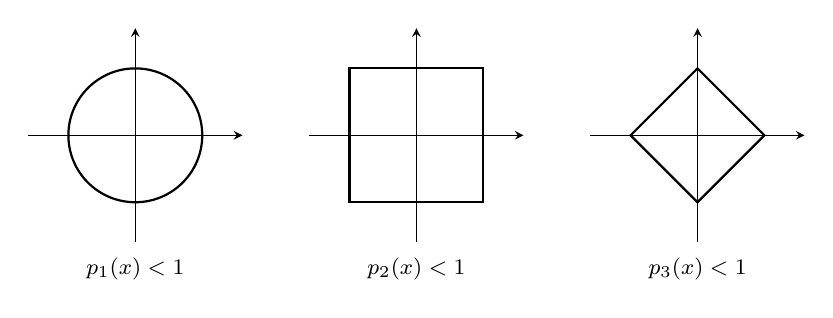
\begin{tikzpicture}[scale=0.85, >=stealth]
    % disk
    \begin{scope}
        \draw[->] (-1.6,0) -- (1.6,0);
        \draw[->] (0,-1.6) -- (0,1.6);
        \draw[thick] (0,0) circle (1);
        \node[font=\footnotesize] at (0,-2) {$p_1(x) < 1$};
    \end{scope}
    % square
    \begin{scope}[xshift=4.2cm]
        \draw[->] (-1.6,0) -- (1.6,0);
        \draw[->] (0,-1.6) -- (0,1.6);
        \draw[thick] (-1,-1) rectangle (1,1);
        \node[font=\footnotesize] at (0,-2) {$p_2(x) < 1$};
    \end{scope}
    % diamond
    \begin{scope}[xshift=8.4cm]
        \draw[->] (-1.6,0) -- (1.6,0);
        \draw[->] (0,-1.6) -- (0,1.6);
        \draw[thick] (1,0) -- (0,1) -- (-1,0) -- (0,-1) -- cycle;
        \node[font=\footnotesize] at (0,-2) {$p_3(x) < 1$};
    \end{scope}
\end{tikzpicture}
\end{center}

All three sets are convex. This is not a coincidence: there is a correspondence between convex sets and positive homogeneous subadditive functions, to be made precise later in the course. In finite dimensions the picture already suggests it.
\end{exbox}

\subsection{The Hahn--Banach Theorem (Real Version)}

\begin{thmbox}[Hahn--Banach]\boxlabel{thm:hb}
Let $X$ be a linear space over $\mathbb{R}$, and let $p : X \to \mathbb{R}$ be positive homogeneous and subadditive. Let $Y$ be a linear subspace of $X$ and $\ell : Y \to \mathbb{R}$ a linear functional on $Y$ satisfying
\[
\ell(y) \leq p(y) \qquad \text{for all } y \in Y.
\]
Then $\ell$ can be extended to a linear functional on $X$: there is a linear functional $L : X \to \mathbb{R}$ with $L|_Y = \ell$ and
\[
L(x) \leq p(x) \qquad \text{for all } x \in X.
\]
\laxref{\S3.1, Thm~1}
\end{thmbox}

\begin{notebox}[Notation]\label{note:notation-2}
Throughout these notes a functional given on a subspace is written $\ell$ and its extension $L$. Wu and Lax keep the name $\ell$ for the extension; the distinction is kept here because several proofs manipulate both at once.
\end{notebox}

The proof is given in \ref{sec:hb-proof}. The complex version will be stated later.

\begin{rembox}[Reading the Statement]\label{rem:reading-statement}
The data are: a linear space $X$; a function $p$ on all of $X$ that behaves like a norm; a linear functional $\ell$ defined only on a subspace $Y$; and a compatibility condition $\ell \leq p$ on $Y$. The conclusion is that $\ell$ extends linearly to an $L$ on all of $X$ without ever exceeding $p$. Since we have no way to write down linear functionals on an abstract $X$ directly (contrast with $\mathbb{R}^n$), the theorem is the fundamental device for producing them: define $\ell$ on a small subspace where it is understood, dominate it by $p$, and extend.
\end{rembox}

\subsection{Geometric Meaning: Hyperplanes and Half-Spaces}

\begin{exbox}[Level Sets of Linear Functionals on $\mathbb{R}^n$]\boxlabel{ex:level-sets-linear-functionals-rn}
Let $\ell(x) = a \cdot x$ on $\mathbb{R}^n$ with $a \neq 0$.
\begin{itemize}
    \item $\{ \ell(x) = 0 \}$ is the set of vectors perpendicular to $a$: a plane through the origin (for $n = 3$).
    \item $\{ \ell(x) = c \}$ is a plane not necessarily through the origin, parallel to the previous one.
    \item $\{ \ell(x) < c \}$ and $\{ \ell(x) > c \}$ are the two sides of that plane; if $a$ points ``upward,'' then $\{\ell < c\}$ is everything below the plane and $\{\ell > c\}$ everything above.
\end{itemize}
\end{exbox}

\begin{defbox}[Hyperplane; Half-Space]\boxlabel{def:hyperplane}
Let $\ell$ be a nonzero linear functional on a linear space $X$ over $\mathbb{R}$ and $c \in \mathbb{R}$. The set $\{ x \in X : \ell(x) = c \}$ is called a \textbf{hyperplane}, and the sets $\{ \ell(x) < c \}$, $\{ \ell(x) > c \}$ are the two \textbf{half-spaces} it bounds.
\laxref{\S3.2, hyperplanes}
\end{defbox}

\begin{rembox}\label{rem:hb-statement-2}
Linear functionals are thus directly tied to geometry: a linear functional and a constant determine a hyperplane and its two half-spaces. Combined with the Hahn--Banach theorem, this is what makes it possible to separate convex sets by hyperplanes in general linear spaces, a theme that will recur.
\end{rembox}


% ============================================================================
% SECTION 4: PROOF OF HAHN-BANACH
% ============================================================================
% Lecture 2 (2026-09-03)

\section{Proof of the Hahn--Banach Theorem}\label{sec:hb-proof}

\roadmark{Stage: algebra}{Thread: functionals. One-step extension, then Zorn's lemma.}

\subsection{Why Linear Functionals}

Before the proof, two remarks on why the set of linear functionals on $X$ is worth studying at all.

\begin{rembox}[Linear Functionals Replace the Dot Product]\label{rem:linear-functionals-replace-dot-product}
On $\mathbb{R}^n$ every linear functional is $x \mapsto a \cdot x$ for a unique $a \in \mathbb{R}^n$, so vectors and linear functionals are in one-to-one correspondence $a \leftrightarrow \ell_a$. Statements about the dot product translate into statements about linear functionals: $a \cdot x = 0$ says $x$ is perpendicular to $a$, and ``$a \cdot x = 0$ for every $a$ implies $x = 0$'' (take $a = x$) says that a vector perpendicular to everything is zero.

A general linear space has no dot product. But it does have linear functionals, and the correspondence above suggests using them as the substitute: ``$x$ is perpendicular to $\ell$'' means $\ell(x) = 0$, and the question of whether ``$\ell(x) = 0$ for all $\ell$ forces $x = 0$'' becomes a question about how many linear functionals exist. The Hahn--Banach theorem is what guarantees there are enough of them.
\end{rembox}

\begin{rembox}[Convergence Without Topology]\label{rem:convergence-without-topology}
A linear space carries no notion of distance, so for a sequence $\{x_n\} \subset X$ the statement ``$x_n \to x$'' has no meaning. But for a linear functional $\ell$, the sequence $\ell(x_n)$ is a sequence of scalars, and convergence of scalars is understood. So linear functionals let one speak of a sequence in $X$ converging, at least in the sense that $\ell(x_n) \to \ell(x)$ for the functionals $\ell$ under consideration. This will be developed later in the course (weak convergence).
\end{rembox}

\subsection{A First Application: One Functional per Vector}

The theorem is a \emph{construction} device. The simplest use:

\begin{exbox}[Extending from a Line]\boxlabel{ex:extending-line}
Let $y_0 \in X$, $y_0 \neq 0$, and let $Y = \operatorname{span}\{y_0\} = \{ a y_0 \mid a \in \mathbb{R} \}$. Define $\ell$ on $Y$ by
\[
\ell(a y_0) = a, \qquad \text{i.e.\ } \ell(y_0) = 1.
\]
This is a linear functional on the one-dimensional subspace $Y$. Given any positive homogeneous subadditive $p$ on $X$ with $\ell(y) \le p(y)$ on $Y$, Hahn--Banach extends $\ell$ to a linear functional $L : X \to \mathbb{R}$ with $L \le p$ on all of $X$. (One can prescribe any value at $y_0$, not only $1$; the normalization is a convenience.)

Thus associated to every nonzero vector of $X$ there is at least one linear functional on $X$ taking a prescribed nonzero value there. The extension is not unique.
\end{exbox}

\subsection{The One-Step Extension}

The whole proof is a single computation: extend $\ell$ by one dimension while keeping $\ell \le p$. Everything else is bookkeeping.

\begin{lembox}[One-Step Extension]\boxlabel{lem:one-step}
Let $X$, $p$, $Y$, $\ell$ be as in Theorem~\ref{thm:hb}, and suppose $Y \subsetneq X$. Fix $x_0 \in X \setminus Y$ and let
\[
Z = \operatorname{span}\{x_0, Y\} = \{ a x_0 + y \mid a \in \mathbb{R},\ y \in Y \}.
\]
Then $\ell$ extends to a linear functional on $Z$: there is a linear $L : Z \to \mathbb{R}$ with $L|_Y = \ell$ and $L(z) \le p(z)$ for all $z \in Z$.

\begin{center}
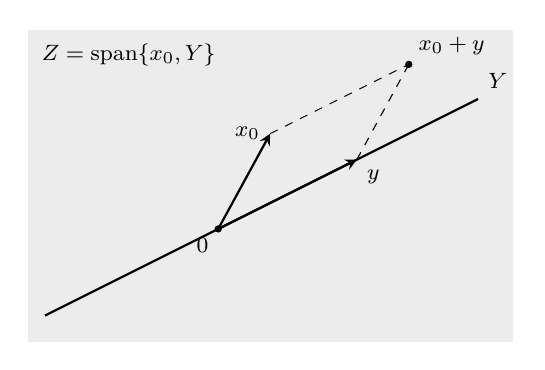
\begin{tikzpicture}[scale=1.1, >=stealth]
    \fill[gray!15] (-2.2,-1.3) rectangle (3.4,2.3);
    \node[font=\footnotesize, anchor=north west] at (-2.15,2.25) {$Z = \operatorname{span}\{x_0, Y\}$};
    \draw[thick] (-2.0,-1.0) -- (3.0,1.5) node[above right] {$Y$};
    \draw[->, thick] (0,0) -- (0.6,1.1) node[left] {$x_0$};
    \draw[->, thick] (0,0) -- (1.6,0.8) node[below right] {$y$};
    \draw[dashed] (1.6,0.8) -- (2.2,1.9);
    \draw[dashed] (0.6,1.1) -- (2.2,1.9);
    \fill (2.2,1.9) circle (1.2pt) node[above right, font=\footnotesize] {$x_0 + y$};
    \fill (0,0) circle (1.2pt) node[below left, font=\footnotesize] {$0$};
\end{tikzpicture}
\end{center}
Pictured for $\dim Y = 1$: $Y$ is a line, $x_0$ is off it, and $Z$ is the plane they span. Every element of $Z$ is $a x_0 + y$ for a unique $a$ and $y$.
\laxref{\S3.1, proof of Thm~1}
\end{lembox}

\begin{proof}
\textbf{Step 1: Reduction to a single number.} First, $Z$ is as described: sums and scalar multiples of elements $a x_0 + y$ are again of that form, so the set of such elements is a subspace containing $x_0$ and $Y$, and it is clearly the smallest one. Moreover the representation $z = a x_0 + y$ is unique: if $a x_0 + y = a' x_0 + y'$ then $(a - a') x_0 = y' - y \in Y$, and since $x_0 \notin Y$ this forces $a = a'$, hence $y = y'$.

Any linear extension $L$ of $\ell$ to $Z$ must satisfy
\[
L(a x_0 + y) = a\, L(x_0) + \ell(y),
\]
and $\ell(y)$ is already known. So the extension is determined by the single real number $c := L(x_0)$, and conversely any choice of $c$ defines a linear functional on $Z$ by this formula (well defined by uniqueness of the representation). The problem is to choose $c$ so that
\begin{equation}\label{eq:hb-want}
L(a x_0 + y) \le p(a x_0 + y) \qquad \text{for all } y \in Y,\ a \in \mathbb{R}.
\end{equation}

\textbf{Step 2: It suffices to treat $a = 1$ and $a = -1$.} We claim it is enough to arrange
\begin{align}
L(x_0 + y) &\le p(x_0 + y) \qquad \text{for all } y \in Y, \tag{1} \label{eq:hb1} \\
L(-x_0 + y') &\le p(-x_0 + y') \qquad \text{for all } y' \in Y. \tag{2} \label{eq:hb2}
\end{align}
The reason is positive homogeneity: $p(ax) = a\,p(x)$ lets a positive scalar be pulled out of $p$, and linearity lets any scalar be pulled out of $L$, so the case of general $a > 0$ reduces to $a = 1$ and the case $a < 0$ reduces to $a = -1$. We cannot pull a negative scalar through $p$, which is why both signs are needed. The verification is Step 5.

\textbf{Step 3: What \eqref{eq:hb1} and \eqref{eq:hb2} say about $c$.} By linearity of $L$ and $L|_Y = \ell$,
\begin{align*}
\eqref{eq:hb1} &\iff c + \ell(y) \le p(x_0 + y) \ \ \forall y \in Y \iff c \le p(x_0 + y) - \ell(y) \ \ \forall y \in Y, \\
\eqref{eq:hb2} &\iff -c + \ell(y') \le p(-x_0 + y') \ \ \forall y' \in Y \iff \ell(y') - p(-x_0 + y') \le c \ \ \forall y' \in Y.
\end{align*}
Together:
\begin{equation}\tag{3}\label{eq:hb3}
\ell(y') - p(-x_0 + y') \;\le\; c \;\le\; p(x_0 + y) - \ell(y) \qquad \text{for all } y, y' \in Y.
\end{equation}
So if $c = L(x_0)$ can be chosen at all, it must satisfy \eqref{eq:hb3}. Note that both outer expressions are well defined: $\ell$ is given on $Y$, and $p$ is given on $X$. The question is whether the two sides leave any room for $c$.

\textbf{Step 4: The sandwich is nonempty.} We show
\begin{equation}\tag{4}\label{eq:hb4}
\ell(y') - p(-x_0 + y') \le p(x_0 + y) - \ell(y) \qquad \text{for all } y, y' \in Y.
\end{equation}
Moving the $\ell$-terms to the left and the $p$-terms to the right, \eqref{eq:hb4} is equivalent to
\[
\ell(y') + \ell(y) \le p(-x_0 + y') + p(x_0 + y).
\]
Now $y' + y \in Y$, so by linearity of $\ell$ on $Y$, the hypothesis $\ell \le p$ on $Y$, and subadditivity of $p$,
\[
\ell(y') + \ell(y) = \ell(y' + y) \le p(y' + y) = p\bigl((y' - x_0) + (x_0 + y)\bigr) \le p(y' - x_0) + p(x_0 + y),
\]
which is the desired inequality. Hence \eqref{eq:hb4} holds.

Fix $y \in Y$ and take the supremum over $y' \in Y$ on the left of \eqref{eq:hb4}: the set $\{\ell(y') - p(-x_0 + y') : y' \in Y\}$ is nonempty and bounded above by $p(x_0 + y) - \ell(y)$, so
\[
c := \sup_{y' \in Y} \bigl( \ell(y') - p(-x_0 + y') \bigr)
\]
is a finite real number with $c \le p(x_0 + y) - \ell(y)$ for every $y \in Y$. Being a supremum, $c \ge \ell(y') - p(-x_0 + y')$ for every $y' \in Y$. Thus $c$ satisfies \eqref{eq:hb3}. (Equally one could take the infimum of the right-hand side of \eqref{eq:hb4} over $y$, or any number in between; the choice is not unique.)

We now \emph{define} $L(x_0) := c$ and, for $a \in \mathbb{R}$, $y \in Y$,
\[
L(a x_0 + y) := a\, c + \ell(y).
\]
By Step 1 this $L$ is a well-defined linear functional on $Z$ extending $\ell$, and by Step 3 it satisfies \eqref{eq:hb1} and \eqref{eq:hb2}.

\textbf{Step 5: Verification of \eqref{eq:hb-want} for all $a$.} For $a = 0$, $\ell(y) \le p(y)$ is the hypothesis.

\emph{Case $a > 0$.} Since $y / a \in Y$, linearity of $L$, \eqref{eq:hb1}, and positive homogeneity of $p$ give
\[
L(a x_0 + y) = a\, L\Bigl(x_0 + \frac{y}{a}\Bigr) \le a\, p\Bigl(x_0 + \frac{y}{a}\Bigr) = p(a x_0 + y).
\]

\emph{Case $a < 0$.} Now $-a > 0$ is the scalar that can be pulled through $p$. Since $y / (-a) \in Y$, linearity, \eqref{eq:hb2}, and positive homogeneity give
\[
L(a x_0 + y) = (-a)\, L\Bigl(-x_0 + \frac{y}{-a}\Bigr) \le (-a)\, p\Bigl(-x_0 + \frac{y}{-a}\Bigr) = p(a x_0 + y).
\]
This proves \eqref{eq:hb-want}, and $\ell$ has been extended to $L$ on $Z$, one dimension larger than $Y$.
\end{proof}

\begin{rembox}[On the Choice of $L(x_0)$]\label{rem:choice-l-x0}
A question in lecture: does taking a supremum preserve linearity? The supremum is not used to define a function; it produces a single real number $c$, which is then assigned as the value $L(x_0)$. Linearity is imposed afterwards by the formula $L(a x_0 + y) = a c + \ell(y)$. Any number in the interval \eqref{eq:hb3} would do; the supremum is merely a convenient way of exhibiting one.

Also note the discipline in Step 3: the conditions \eqref{eq:hb1}, \eqref{eq:hb2} were converted to conditions on $c$ by \emph{equivalences}, not by one-sided estimates. Applying subadditivity too early would have thrown away information and made the interval for $c$ harder to see.
\end{rembox}

\subsection{Completing the Proof: Zorn's Lemma}

\begin{thmbox}[Zorn's Lemma]\boxlabel{thm:zorn}
Let $(P, \le)$ be a nonempty partially ordered set in which every chain (totally ordered subset) has an upper bound in $P$. Then $P$ has a maximal element, i.e.\ an $m \in P$ with no $x \in P$ satisfying $m < x$.
\laxref{\S3.1, proof of Thm~1}
\end{thmbox}

Zorn's lemma is equivalent to the axiom of choice and is taken as an axiom; no proof is given. Wu stated in lecture that the partial-order argument would not be carried out on the board; it is written out here.

\begin{proof}[Proof of Theorem~\ref{thm:hb}]
(Wu: ``By Zorn's lemma, we're done.'' The argument is written out here.) If $Y = X$ there is nothing to do, so assume $Y \subsetneq X$. Let $P$ be the set of pairs $(Z, \ell_Z)$ with $Y \subset Z \subset X$ a linear subspace and $\ell_Z : Z \to \mathbb{R}$ a linear functional extending $\ell$ with $\ell_Z \le p$ on $Z$, ordered by extension: $(Z, \ell_Z) \le (Z', \ell_{Z'})$ iff $Z \subset Z'$ and $\ell_{Z'}|_Z = \ell_Z$. Then $(Y, \ell) \in P$, so $P \neq \varnothing$.

\emph{Chains have upper bounds.} Given a chain $\{(Z_i, \ell_i)\}_{i \in I}$, let $Z^* = \bigcup_i Z_i$ and define $\ell^*(z) = \ell_i(z)$ for any $i$ with $z \in Z_i$. Since the chain is nested, any two elements of $Z^*$ lie in a common $Z_i$, so $Z^*$ is a subspace and $\ell^*$ is well defined and linear; $\ell^* \le p$ on $Z^*$ because it holds on each $Z_i$. Thus $(Z^*, \ell^*) \in P$ is an upper bound.

\emph{Conclusion.} By Zorn's lemma $P$ has a maximal element $(Z_m, \ell_m)$. If $Z_m \neq X$, Lemma~\ref{lem:one-step} (with $Z_m$ in place of $Y$) extends $\ell_m$ to a strictly larger subspace keeping $\ell \le p$, contradicting maximality. Hence $Z_m = X$, and $L := \ell_m$ is the required extension.
\end{proof}

\begin{rembox}\label{rem:hb-proof}
Lemma~\ref{lem:one-step} contains all the analysis; Zorn's lemma only says ``repeat until finished'' in a way that is legitimate when $X$ has uncountable dimension. In separable normed spaces (later) the extension can instead be built by ordinary induction along a countable dense sequence.
\end{rembox}

% ============================================================================
% SECTION 5: CONVEX SETS AND THE GAUGE
% ============================================================================

\section{Convex Sets and the Gauge}\label{sec:gauge}

\roadmark{Stage: algebra}{Thread: convexity. Convex sets and positive homogeneous subadditive functions are two descriptions of one object.}

The three functions $p_1, p_2, p_3$ on $\mathbb{R}^n$ each came with a convex set $\{p < 1\}$. This is the beginning of a two-way correspondence between positive homogeneous subadditive functions and convex sets, which is what makes Hahn--Banach a geometric theorem.

\subsection{From $p$ to a Convex Set}

\begin{propbox}[Positive Homogeneous Subadditive $p$ Gives a Convex Set]\boxlabel{prop:sublevel-convex}
Let $p : X \to \mathbb{R}$ be positive homogeneous and subadditive, and let
\[
K = \{ x \in X : p(x) \le 1 \}, \qquad K_0 = \{ x \in X : p(x) < 1 \}.
\]
Then $K$ and $K_0$ are convex.
\laxref{\S3.1, Thm~4}
\end{propbox}

\begin{proof}
(HW1.) Let $x_1, x_2 \in K$ and $a \in [0,1]$. If $a = 0$ or $a = 1$ the point $a x_1 + (1-a) x_2$ is $x_2$ or $x_1$, which lies in $K$. For $0 < a < 1$, subadditivity followed by positive homogeneity (with the non-negative scalars $a$ and $1 - a$) gives
\[
p\bigl(a x_1 + (1-a) x_2\bigr) \le p(a x_1) + p\bigl((1-a) x_2\bigr) = a\,p(x_1) + (1-a)\,p(x_2) \le a \cdot 1 + (1-a) \cdot 1 = 1,
\]
so $a x_1 + (1-a) x_2 \in K$. For $K_0$ the same chain ends with $< a \cdot 1 + (1-a) \cdot 1 = 1$, strict because $p(x_1) < 1$, $p(x_2) < 1$ and both weights $a, 1-a$ are positive; the endpoint cases $a \in \{0,1\}$ are handled as before.
\end{proof}

\begin{rembox}\label{rem:gauge}
On the board the set was written with $\le 1$; the homework uses $< 1$. Nothing in the convexity argument distinguishes the two, but they play different roles later: $K_0$ is the set all of whose points are interior (Proposition~\ref{prop:open-interior}), and it is $K_0$, not $K$, that will be recovered from the gauge as $\{p_K < 1\}$. Both contain $0$, since $p(0) = 0$ (Lemma~\ref{lem:p-zero}).
\end{rembox}

The converse direction --- starting from a convex set and producing a $p$ --- is the gauge, below. It requires a notion of interior point that makes sense without any topology.

\subsection{Interior Points, Algebraically}

\begin{defbox}[Interior Point]\boxlabel{def:interior}
Let $K \subset X$ be a subset of a linear space and $x_0 \in K$. We say $x_0$ is an \textbf{interior point} of $K$ if for every $y \in X$ there exists $\varepsilon = \varepsilon(y) > 0$ such that
\[
x_0 + t y \in K \qquad \text{for all } |t| < \varepsilon(y).
\]
\laxref{\S3.1, definition of interior point}
\end{defbox}

\begin{rembox}[Comparison with the Classical Notion]\label{rem:comparison-classical-notion}
In a metric space, $x_0$ is an interior point of $K$ if some ball around $x_0$ lies in $K$. Here there is no ball. The definition says instead: in every direction $y$, one can move a little way from $x_0$ (in both senses, $t > 0$ and $t < 0$) and stay inside $K$. The allowed distance $\varepsilon(y)$ depends on the direction and is not uniform: $K$ may be very thin in one direction and long in another, and there need be no single $\varepsilon$ that works for all $y$. Whenever both notions make sense, an interior point in the classical sense is one in this sense, but not conversely (Proposition~\ref{prop:metric-interior} and the example after it); this is the only notion available in a bare linear space.

\begin{center}
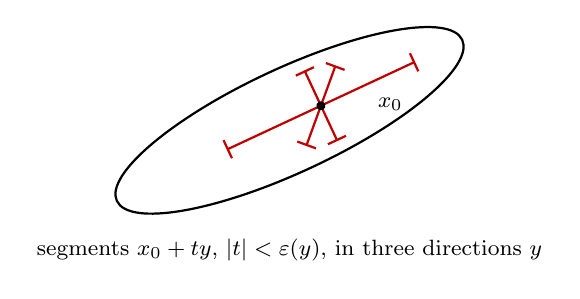
\begin{tikzpicture}[scale=1.1, >=stealth]
    \begin{scope}[rotate=25]
        \draw[thick] (0,0) ellipse (2.2 and 0.6);
        \coordinate (x0) at (0.4,0);
        \draw[thick, red!75!black, |-|] ($(x0)+(-1.2,0)$) -- ($(x0)+(1.2,0)$);
        \draw[thick, red!75!black, |-|] ($(x0)+(0,-0.45)$) -- ($(x0)+(0,0.45)$);
        \draw[thick, red!75!black, |-|] ($(x0)+(-0.35,-0.35)$) -- ($(x0)+(0.35,0.35)$);
        \fill (x0) circle (1.5pt);
        \node[anchor=west, font=\footnotesize] at ($(x0)+(0.5,-0.22)$) {$x_0$};
    \end{scope}
    \node[font=\footnotesize] at (0,-1.5) {segments $x_0 + t y$, $|t| < \varepsilon(y)$, in three directions $y$};
\end{tikzpicture}
\end{center}
\end{rembox}

\begin{propbox}[{{Every Point of $\{p < 1\}$ is Interior}}]\boxlabel{prop:open-interior}
Let $p : X \to \mathbb{R}$ be positive homogeneous and subadditive, and $K_0 = \{ x \in X : p(x) < 1 \}$. Then every point of $K_0$ is an interior point of $K_0$.
\laxref{\S3.1, Thm~4(i)}
\end{propbox}

\begin{proof}
(Not reached in lecture; written out here.) Let $x \in K_0$, so $p(x) < 1$, and let $y \in X$. Put $M = \max\{p(y), p(-y), 0\}$, a finite non-negative number, and choose
\[
\varepsilon(y) = \frac{1 - p(x)}{M + 1} > 0.
\]
For $|t| < \varepsilon(y)$, write $ty = |t| \cdot (\pm y)$ with the sign of $t$. By subadditivity and positive homogeneity,
\[
p(x + ty) \le p(x) + |t|\,p(\pm y) \le p(x) + |t| M < p(x) + \varepsilon(y)(M+1) = 1,
\]
so $x + ty \in K_0$. Hence $x$ is an interior point of $K_0$. (The $+1$ in the denominator only avoids dividing by $0$ when $M = 0$.)
\end{proof}

\begin{rembox}[Comparison with Lax]\label{rem:comparison-lax-2}
Lax's Theorem~4(i) asserts only that $0$ is an interior point of $\{p < 1\}$, leaving the rest as an exercise. The stronger statement proved here, that every point is interior, is what Corollary~\ref{cor:sublevel} and the separation theorem use.
\end{rembox}

\subsection{The Gauge of a Convex Set}

\begin{defbox}[Gauge]\boxlabel{def:gauge}
Let $K$ be a convex set in a linear space $X$ with $0$ an interior point of $K$. The \textbf{gauge} (or Minkowski functional) associated with $K$ is
\[
p_K(x) = \inf\Bigl\{ a > 0 \;:\; \frac{x}{a} \in K \Bigr\}, \qquad x \in X.
\]
\laxref{\S3.1, equation (8)}
\end{defbox}

\begin{propbox}[The Gauge is Finite]\boxlabel{prop:gauge-finite}
Under the hypotheses of the definition, the set $\{a > 0 : x/a \in K\}$ is nonempty for every $x \in X$, so $p_K(x) < \infty$. More precisely, if $\varepsilon(x) > 0$ is as in the definition of $0$ being an interior point, then $p_K(x) \le 1/\varepsilon(x)$.
\end{propbox}

\begin{proof}
Fix $x \in X$. Since $0$ is an interior point of $K$, there is $\varepsilon(x) > 0$ such that $t x \in K$ for all $|t| < \varepsilon(x)$. Take any $t$ with $0 < t < \varepsilon(x)$. Then $t x = x / (1/t) \in K$, so $a = 1/t$ belongs to the set in the definition of $p_K$, and therefore $p_K(x) \le 1/t$. Since this holds for every $t \in (0, \varepsilon(x))$, letting $t \uparrow \varepsilon(x)$ gives $p_K(x) \le 1/\varepsilon(x) < \infty$.
\end{proof}

\begin{rembox}\label{rem:gauge-2}
$p_K(x)$ measures how far $x$ must be shrunk toward the origin to land in $K$: $x / a \in K$ for all $a$ larger than $p_K(x)$, and for no $a$ smaller. Small $p_K(x)$ means $x$ is well inside $K$ (or that $K$ extends far in the direction of $x$); large $p_K(x)$ means $x$ is far outside. For $x = 0$ every $a > 0$ is admissible, so $p_K(0) = 0$. Note also that $p_K \ge 0$ by construction, unlike a general positive homogeneous subadditive $p$ (both facts are Proposition~\ref{prop:gauge-values}(a) below).

\begin{center}
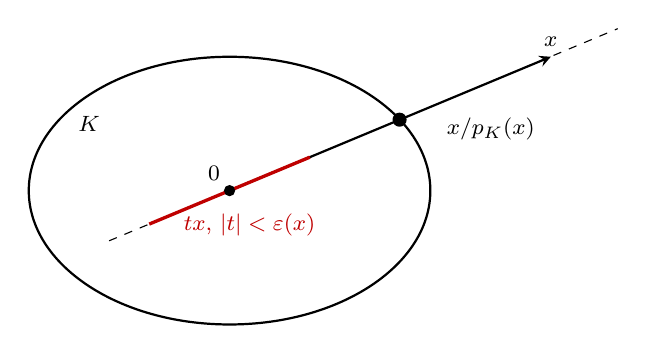
\begin{tikzpicture}[scale=1.7, >=stealth]
    \draw[thick] (0,0) ellipse (1.5 and 1.0);
    \node[font=\footnotesize] at (-1.05,0.5) {$K$};
    \draw[dashed] (-0.9,-0.375) -- (2.9,1.21);
    \draw[->, thick] (0,0) -- (2.4,1.0) node[above, font=\footnotesize] {$x$};
    \draw[very thick, red!75!black] (-0.6,-0.25) -- (0.6,0.25);
    \node[below, font=\footnotesize, red!75!black] at (0.15,-0.1) {$tx$, $|t|<\varepsilon(x)$};
    \fill (1.27,0.53) circle (1.5pt);
    \node[anchor=west, font=\footnotesize] at (1.55,0.46) {$x / p_K(x)$};
    \fill (0,0) circle (1.2pt) node[above left, font=\footnotesize] {$0$};
\end{tikzpicture}
\end{center}
Along the ray through $x$, the points $tx$ with $t$ small lie in $K$ (this is $0$ being interior, and gives $p_K(x) \le 1/\varepsilon(x)$); the point where the ray leaves $K$ is $x / p_K(x)$.
\end{rembox}

\subsection{The Admissible Set and the Values of the Gauge}

The material of this subsection was not covered in lecture; it makes precise the picture above.

\begin{notebox}[Notation]\label{note:notation-3}
For $K$ as in the definition of the gauge and $x \in X$, write
\[
A(x) = \{ a > 0 : x/a \in K \},
\]
so that $p_K(x) = \inf A(x)$. Proposition~\ref{prop:gauge-finite} says $A(x) \neq \varnothing$.
\end{notebox}

\begin{lembox}[Admissible Scales Form an Upper Set]\boxlabel{lem:upset}
If $a \in A(x)$ and $a' > a$, then $a' \in A(x)$. Consequently $A(x)$ is an interval of the form $[p_K(x), \infty)$ or $(p_K(x), \infty)$.
\end{lembox}

\begin{proof}
Write $\lambda = a/a' \in (0,1)$. Then
\[
\frac{x}{a'} = \lambda \cdot \frac{x}{a} + (1 - \lambda) \cdot 0,
\]
a convex combination of $x/a \in K$ and $0 \in K$. By convexity of $K$, $x/a' \in K$, i.e.\ $a' \in A(x)$. Thus $A(x)$ contains every number larger than any of its elements; together with $\inf A(x) = p_K(x)$ this gives the stated form, the endpoint being included exactly when $x / p_K(x) \in K$.
\end{proof}

Both hypotheses on $K$ are used: convexity for the combination, and $0 \in K$ (which follows from $0$ being interior) for the second term.

\begin{propbox}[Values of the Gauge]\boxlabel{prop:gauge-values}
Let $K$ be convex with $0$ an interior point, and $x \in X$.
\begin{enumerate}[label=(\alph*)]
    \item $p_K(x) \ge 0$, and $p_K(0) = 0$.
    \item If $x \in K$ then $p_K(x) \le 1$; if $x \notin K$ then $p_K(x) \ge 1$.
    \item $p_K(x) = 0$ if and only if the whole ray $\{ sx : s \ge 0 \}$ lies in $K$.
\end{enumerate}
\laxref{\S3.1, Thm~3, (10)}
\end{propbox}

\begin{proof}
(a) $A(x) \subset (0, \infty)$, so its infimum is $\ge 0$. For $x = 0$, $0/a = 0 \in K$ for every $a > 0$, so $A(0) = (0,\infty)$ and $p_K(0) = 0$.

(b) If $x \in K$ then $1 \in A(x)$, so $p_K(x) \le 1$. If $x \notin K$ then $1 \notin A(x)$, and by Lemma~\ref{lem:upset} no $a \le 1$ lies in $A(x)$ either (if some $a \le 1$ did, then $1 \ge a$ would). Hence $A(x) \subset (1, \infty)$ and $p_K(x) \ge 1$.

(c) $p_K(x) = 0$ iff $A(x)$ contains arbitrarily small $a > 0$, iff (by Lemma~\ref{lem:upset}) $A(x) = (0,\infty)$, iff $x/a \in K$ for all $a > 0$, iff $sx \in K$ for all $s > 0$; and $s = 0$ is included since $0 \in K$.
\end{proof}

\begin{rembox}[Reading the Cases]\label{rem:reading-cases}
Positive homogeneity (Proposition~\ref{prop:gauge-sublinear} below, $p_K(tx) = t\,p_K(x)$) says the gauge is not constant along a ray but \emph{linear} along it: what is constant is the exit point $x^* = x / p_K(x)$ at which the ray through $x$ leaves $K$ (when $p_K(x) > 0$), and $p_K(x)$ counts how many copies of $x^*$ make up $x$.

The two halves of (b) are the same statement seen from opposite sides. In both, $p_K(x)$ is the scale $a$ at which $x/a$ sits on the boundary of $K$:
\begin{itemize}
    \item \emph{$x$ outside $K$.} Dividing by $a$ must \emph{shrink} $x$, so $a$ increases from $1$; the points $x/a$ move along the ray toward $0$ and enter $K$ at $a = p_K(x) \ge 1$. Every larger $a$ is admissible (Lemma~\ref{lem:upset}); no smaller $a$ is, since shrinking can only bring $x$ into $K$, never take it out. The crossing scale is the infimum.
    \item \emph{$x$ inside $K$.} Dividing by $a$ must \emph{stretch} $x$, so $a$ decreases from $1$; the points $x/a$ move outward and reach the boundary at $a = p_K(x) \le 1$. Every $a$ above this is admissible, no $a$ below it is, and again the crossing scale is the infimum.
\end{itemize}

\begin{center}
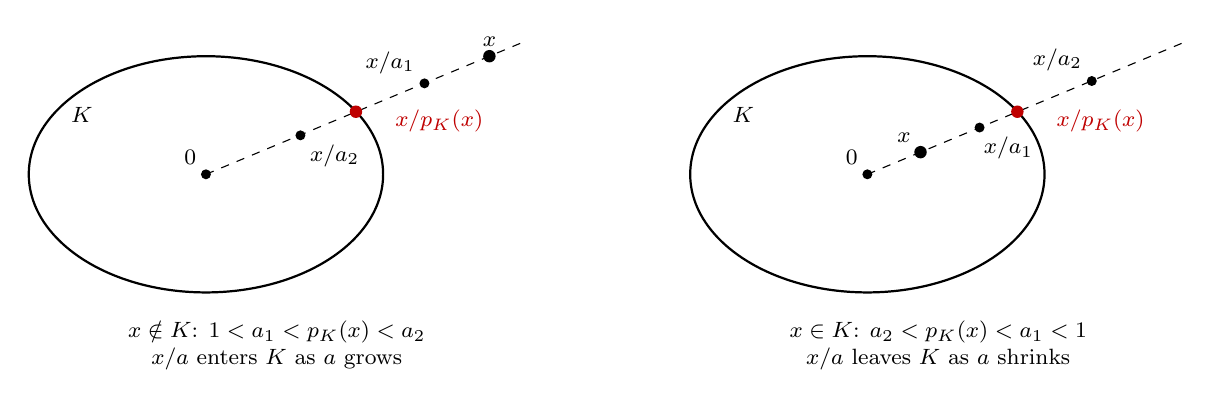
\begin{tikzpicture}[scale=1.5, >=stealth]
    % left: x outside
    \begin{scope}
        \draw[thick] (0,0) ellipse (1.5 and 1.0);
        \node[font=\footnotesize] at (-1.05,0.5) {$K$};
        \draw[dashed] (0,0) -- (2.7,1.125);
        \fill (0,0) circle (1.2pt) node[above left, font=\footnotesize] {$0$};
        \fill (2.4,1.0) circle (1.5pt) node[above, font=\footnotesize] {$x$};
        \fill (1.85,0.77) circle (1.2pt) node[above left, font=\footnotesize] {$x/a_1$};
        \fill[red!75!black] (1.27,0.53) circle (1.5pt);
        \fill (0.8,0.33) circle (1.2pt) node[below right, font=\footnotesize] {$x/a_2$};
        \node[anchor=west, font=\footnotesize, red!75!black] at (1.52,0.45) {$x/p_K(x)$};
        \node[font=\footnotesize, align=center] at (0.6,-1.45) {$x \notin K$: $1 < a_1 < p_K(x) < a_2$ \\ $x/a$ enters $K$ as $a$ grows};
    \end{scope}
    % right: x inside
    \begin{scope}[xshift=5.6cm]
        \draw[thick] (0,0) ellipse (1.5 and 1.0);
        \node[font=\footnotesize] at (-1.05,0.5) {$K$};
        \draw[dashed] (0,0) -- (2.7,1.125);
        \fill (0,0) circle (1.2pt) node[above left, font=\footnotesize] {$0$};
        \fill (0.45,0.1875) circle (1.5pt) node[above left, font=\footnotesize] {$x$};
        \fill (0.95,0.396) circle (1.2pt) node[below right, font=\footnotesize, xshift=-2pt] {$x/a_1$};
        \fill[red!75!black] (1.27,0.53) circle (1.5pt);
        \fill (1.9,0.79) circle (1.2pt) node[above left, font=\footnotesize] {$x/a_2$};
        \node[anchor=west, font=\footnotesize, red!75!black] at (1.52,0.45) {$x/p_K(x)$};
        \node[font=\footnotesize, align=center] at (0.6,-1.45) {$x \in K$: $a_2 < p_K(x) < a_1 < 1$ \\ $x/a$ leaves $K$ as $a$ shrinks};
    \end{scope}
\end{tikzpicture}
\end{center}

Two refinements. Whether the crossing scale itself belongs to $A(x)$ depends on whether the boundary point belongs to $K$: for the closed disk $A(x) = [\|x\|, \infty)$, for the open disk $A(x) = (\|x\|, \infty)$; the infimum is the same. And ``until the edge'' presupposes that the ray exits $K$. If it does not (part (c), and the example below), there is no edge to reach, $a$ can decrease all the way to $0$, and $p_K(x) = 0$ with $x \neq 0$. So $p_K(x) = 0$ does not force $x = 0$; exactly when a gauge is a norm is settled in Proposition~\ref{prop:norm-gauge}.
\end{rembox}

\begin{exbox}[A Gauge Vanishing Off the Origin]\boxlabel{ex:gauge-vanishing-off-origin}
Let $X = \mathbb{R}^2$ and $K = \{ (x_1, x_2) : x_1 < 1 \}$, an open half-plane containing $0$ as an interior point. For $x = (x_1, x_2)$ with $x_1 \le 0$, every point $sx$, $s \ge 0$, has first coordinate $sx_1 \le 0 < 1$, so the whole ray lies in $K$ and $p_K(x) = 0$. For $x_1 > 0$, $x/a \in K$ iff $x_1/a < 1$ iff $a > x_1$, so $A(x) = (x_1, \infty)$ and $p_K(x) = x_1$. Altogether $p_K(x) = \max\{x_1, 0\}$: positive homogeneous, subadditive, non-negative, and zero on a whole half-plane.
\end{exbox}

\begin{exbox}[Gauge of the Unit Disk]\boxlabel{ex:gauge-unit-disk}
Let $X = \mathbb{R}^2$ and $K = \{ x_1^2 + x_2^2 \le 1 \}$, the closed unit disk; $0$ is an interior point in the classical sense, hence in the algebraic sense. For $x = (x_1, x_2)$ and $a > 0$,
\[
\frac{x}{a} \in K \iff \Bigl(\frac{x_1}{a}\Bigr)^2 + \Bigl(\frac{x_2}{a}\Bigr)^2 \le 1 \iff a^2 \ge x_1^2 + x_2^2 \iff a \ge \sqrt{x_1^2 + x_2^2}.
\]
The infimum of such $a$ is attained, and
\[
p_K(x) = \bigl(x_1^2 + x_2^2\bigr)^{1/2} = \|x\|.
\]
So the gauge of the unit disk recovers the Euclidean length: the function $p_1$ of Example~\ref{ex:three-p} is the gauge of its own unit ball. Similarly, $p_2$ is the gauge of the square and $p_3$ the gauge of the diamond.
\end{exbox}

% Lecture 3 (2026-09-08)

\begin{exbox}[Gauge of a Square]\boxlabel{ex:gauge-square}
Let $X = \mathbb{R}^2$ and $K = \{ (x_1, x_2) : |x_1| \le 2,\ |x_2| \le 2 \}$, the closed square with vertices $(\pm 2, \pm 2)$; $0$ is an interior point. For $a > 0$,
\[
\frac{x}{a} \in K \iff \Bigl|\frac{x_1}{a}\Bigr| \le 2 \text{ and } \Bigl|\frac{x_2}{a}\Bigr| \le 2 \iff a \ge \frac{|x_1|}{2} \text{ and } a \ge \frac{|x_2|}{2} \iff a \ge \max\Bigl\{\frac{|x_1|}{2}, \frac{|x_2|}{2}\Bigr\}.
\]
Both conditions must hold (``and,'' not ``or''), so the smallest admissible $a$ is the larger of the two lower bounds, and
\[
p_K(x) = \tfrac{1}{2} \max\{ |x_1|, |x_2| \}.
\]
This is the function $p_2$ of Example~\ref{ex:three-p} scaled by $\tfrac12$; the factor records that $K$ is the square of side $4$, not $2$. Once again the gauge is a way of measuring the size of $x$, adapted to the shape of $K$.
\begin{center}
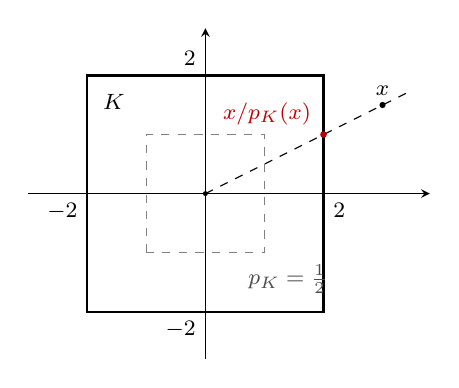
\begin{tikzpicture}[scale=0.75, >=stealth]
    \draw[->] (-3,0) -- (3.8,0);
    \draw[->] (0,-2.8) -- (0,2.8);
    \draw[thick] (-2,-2) rectangle (2,2);
    \draw[dashed, gray] (-1,-1) rectangle (1,1);
    \node[gray!60!black] at (1.4,-1.45) {$p_K = \tfrac12$};
    \node at (-1.55,1.55) {$K$};
    \node[below right] at (2,0) {$2$};
    \node[below left] at (-2,0) {$-2$};
    \node[above left] at (0,2) {$2$};
    \node[below left] at (0,-2) {$-2$};
    \draw[dashed] (0,0) -- (3.5,1.75);
    \fill (0,0) circle (1.2pt);
    \fill (3,1.5) circle (1.5pt) node[above] {$x$};
    \fill[red!75!black] (2,1) circle (1.6pt) node[above left, red!75!black, xshift=-1pt] {$x/p_K(x)$};
\end{tikzpicture}
\end{center}
For $x = (3, \tfrac32)$, $p_K(x) = \tfrac32$ and $x/p_K(x) = (2, 1)$ lies on the boundary. The level sets $\{p_K = c\}$ are the squares of half-side $2c$; the dashed one is $c = \tfrac12$. (The picture drawn in Lecture~3.)
\end{exbox}

\subsection{The Gauge is Positive Homogeneous and Subadditive}

\begin{propbox}[The Gauge is Positive Homogeneous and Subadditive]\boxlabel{prop:gauge-sublinear}
Let $K$ be a convex set in $X$ with $0$ an interior point. Then $p_K$ is positive homogeneous and subadditive:
\[
p_K(bx) = b\, p_K(x) \quad (b \ge 0), \qquad p_K(x + y) \le p_K(x) + p_K(y) \qquad \text{for all } x, y \in X.
\]
\laxref{\S3.1, Thm~2}
\end{propbox}

\begin{proof}
\textbf{Positive homogeneity.} For $b = 0$ both sides are $0$ by Proposition~\ref{prop:gauge-values}(a). For $b > 0$,
\[
p_K(bx) = \inf\Bigl\{ a > 0 : \frac{bx}{a} \in K \Bigr\} = \inf\Bigl\{ a > 0 : \frac{x}{a/b} \in K \Bigr\}.
\]
Substituting $a' = a/b$, which runs over $(0,\infty)$ as $a$ does, the set is $\{ b a' : x/a' \in K \} = b\,A(x)$, whose infimum is $b \inf A(x) = b\, p_K(x)$. (Wu left this check to us.)

\textbf{Subadditivity.} It is hard to work with the infimum directly, so take arbitrary admissible scales and pass to the infimum at the end. Let $a > 0$, $b > 0$ be such that
\[
\frac{x}{a} \in K, \qquad \frac{y}{b} \in K,
\]
so that $p_K(x) \le a$ and $p_K(y) \le b$. It suffices to show $p_K(x + y) \le a + b$, i.e.\ that $\dfrac{x + y}{a + b} \in K$; the claim then follows by taking the infimum over all such $a$, then over all such $b$. Now
\[
\frac{x + y}{a + b} = \frac{a}{a + b} \cdot \frac{x}{a} + \frac{b}{a + b} \cdot \frac{y}{b},
\]
and since $a, b > 0$,
\[
0 < \frac{a}{a+b} < 1, \qquad 0 < \frac{b}{a+b} < 1, \qquad \frac{a}{a+b} + \frac{b}{a+b} = 1.
\]
So $(x + y)/(a + b)$ is a convex combination of the two points $x/a$, $y/b$ of $K$, hence lies in $K$ by convexity. Thus $a + b$ is an admissible scale for $x + y$ and $p_K(x + y) \le a + b$. Taking the infimum over $a \in A(x)$ and then over $b \in A(y)$ gives $p_K(x + y) \le p_K(x) + p_K(y)$.
\end{proof}

\begin{rembox}\label{rem:gauge-3}
The two properties come from the two hypotheses on $K$: positive homogeneity is pure bookkeeping with the definition (it would hold for any $K$ for which the infimum is finite), while subadditivity is convexity, used exactly once, with the convexity coefficients $a/(a+b)$ and $b/(a+b)$. Together with Proposition~\ref{prop:sublevel-convex} this closes the loop: a positive homogeneous subadditive $p$ produces a convex set $\{p < 1\}$, and a convex set (with $0$ interior) produces a positive homogeneous subadditive $p_K$.
\end{rembox}

\subsection{Interior Points via the Gauge}

\begin{propbox}[Interior Points of $K$ are Exactly $\{p_K < 1\}$]\boxlabel{prop:interior-gauge}
Let $K$ be a convex set in $X$ with $0$ an interior point.
\begin{enumerate}[label=(\arabic*)]
    \item For all $x \in K$, $p_K(x) \le 1$.
    \item $x$ is an interior point of $K$ if and only if $p_K(x) < 1$.
\end{enumerate}
\laxref{\S3.1, Thm~3, (10$'$)}
\end{propbox}

\begin{proof}
(1) If $x \in K$ then $x/1 \in K$, so $a = 1$ is admissible and the infimum is at most $1$.

(2) ($\Rightarrow$) Assume $x$ is an interior point of $K$. By (1), $p_K(x) \le 1$; we want strict inequality, i.e.\ some $a < 1$ with $x/a \in K$. Equivalently, it suffices to find $b > 0$ with $(1 + b)x \in K$, for then $a = 1/(1+b) < 1$ works. Apply the definition of interior point to $x$ in the direction $y = x$ itself: there is $\varepsilon(x) > 0$ such that
\[
x + bx \in K \qquad \text{for all } |b| < \varepsilon(x).
\]
In particular $(1 + b)x \in K$ for all $0 < b < \varepsilon(x)$, so
\[
p_K(x) \le \frac{1}{1 + b} < 1.
\]
Being interior means $x$ can be pushed a little in \emph{every} direction, including outward along its own ray; that is all this direction uses.

($\Leftarrow$) Assume $p_K(x) < 1$. By definition of the infimum there is $a$ with $0 < a < 1$ and $x/a \in K$. We must show that for every $y \in X$ there is $\varepsilon(y) > 0$ with $x + ty \in K$ for all $|t| < \varepsilon(y)$.

Fix $y \in X$. Since $0$ is an interior point of $K$, there is $\delta(y) > 0$ such that $ty = 0 + ty \in K$ for all $|t| < \delta(y)$. Now use convexity of $K$ on the two points $x/a \in K$ and $ty \in K$, with coefficients $a$ and $1 - a$ (both in $(0,1)$, summing to $1$):
\[
a \cdot \frac{x}{a} + (1 - a)\, ty \in K, \qquad \text{i.e.} \qquad x + (1 - a)\, t y \in K \qquad \text{for all } |t| < \delta(y).
\]
Replacing $(1-a)t$ by $t$, this says $x + ty \in K$ for all $|t| < (1 - a)\,\delta(y)$. So $\varepsilon(y) = (1 - a)\,\delta(y) > 0$ works, and $x$ is an interior point.
\end{proof}

\begin{center}
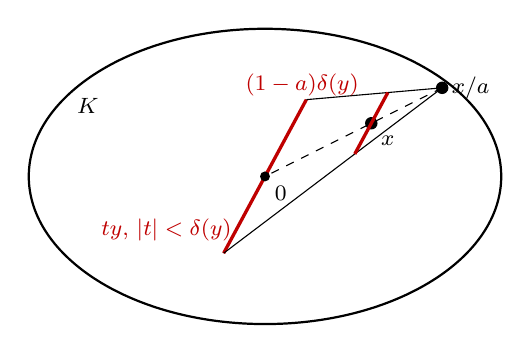
\begin{tikzpicture}[scale=1.5, >=stealth]
    \draw[thick] (0,0) ellipse (2.0 and 1.25);
    \node[font=\footnotesize] at (-1.5,0.6) {$K$};
    % base segment through 0 in direction y (not parallel to x)
    \draw[very thick, red!75!black] (-0.35,-0.65) -- (0.35,0.65);
    \node[left, font=\footnotesize, red!75!black] at (-0.2,-0.45) {$ty$, $|t| < \delta(y)$};
    \fill (0,0) circle (1.2pt) node[below right, font=\footnotesize] {$0$};
    % apex x/a
    \coordinate (apex) at (1.5,0.75);
    \fill (apex) circle (1.5pt) node[right, font=\footnotesize] {$x/a$};
    \draw[thin] (apex) -- (-0.35,-0.65);
    \draw[thin] (apex) -- (0.35,0.65);
    \draw[dashed] (apex) -- (0,0);
    % x on the median at fraction a (a = 0.6)
    \coordinate (x) at (0.9,0.45);
    \fill (x) circle (1.5pt) node[below right, font=\footnotesize, yshift=-1pt] {$x$};
    % cross-section through x parallel to y, half-length (1-a)delta = 0.4*(0.35,0.65)
    \draw[very thick, red!75!black] ($(x)+(-0.14,-0.26)$) -- ($(x)+(0.14,0.26)$);
    \node[above left, font=\footnotesize, red!75!black, xshift=-1pt] at ($(x)+(0.0,0.15)$) {$(1-a)\delta(y)$};
\end{tikzpicture}
\end{center}
The picture behind ($\Leftarrow$): the segment $\{ty : |t| < \delta(y)\}$ through $0$ lies in $K$, the apex $x/a$ lies in $K$, so by convexity the whole triangle they span lies in $K$. The point $x = a \cdot (x/a) + (1-a) \cdot 0$ sits on the median at fraction $a$ from the apex, and the triangle's cross-section through $x$ parallel to $y$ has half-length $(1 - a)\,\delta(y)$. That cross-section is the wiggle room at $x$ in the direction $y$.

\begin{corbox}[Convex Sets of Interior Points are Sublevel Sets]\boxlabel{cor:sublevel}
Let $K \subset X$ be convex with $0 \in K$. The following are equivalent:
\begin{enumerate}[label=(\roman*)]
    \item every point of $K$ is an interior point of $K$;
    \item $K = \{ x \in X : p(x) < 1 \}$ for some positive homogeneous subadditive $p : X \to \mathbb{R}$.
\end{enumerate}
When they hold, one can take $p = p_K$.
\laxref{\S3.1, Thms~3--4}
\end{corbox}

\begin{proof}
(Not covered in lecture.) (ii)$\Rightarrow$(i) is Proposition~\ref{prop:open-interior}. (i)$\Rightarrow$(ii): by (i), $0$ is an interior point, so $p_K$ is defined and is positive homogeneous and subadditive (Proposition~\ref{prop:gauge-sublinear}). Since every point of $K$ is interior, $x \in K$ iff $x$ is an interior point of $K$, iff $p_K(x) < 1$ by Proposition~\ref{prop:interior-gauge}(2).
\end{proof}

\begin{rembox}\label{rem:gauge-4}
The corollary is the converse to Proposition~\ref{prop:sublevel-convex}: the sets $\{p < 1\}$ are exactly the convex sets containing $0$ all of whose points are interior, and each such set is recovered from its own gauge. The hypothesis that $0$ is interior was used in ($\Leftarrow$) of Proposition~\ref{prop:interior-gauge} to get the base segment; without it the gauge is not even defined. This is the form in which the separation theorem uses the gauge.
\end{rembox}

% ============================================================================
% SECTION 6: HYPERPLANE SEPARATION
% ============================================================================

\section{The Hyperplane Separation Theorem}\label{sec:separation}

\roadmark{Stage: algebra}{Threads meet: functionals $\times$ convexity. Hahn--Banach applied to a gauge.}

This is the first application of Hahn--Banach, and the reason the theorem was stated with a general $p$ rather than a norm: the $p$ that gets used is the gauge of a convex set. Recall (Definition~\ref{def:hyperplane}) that for a nonzero linear functional $\ell : X \to \mathbb{R}$ and $c \in \mathbb{R}$, $\{\ell = c\}$ is a hyperplane and $\{\ell < c\}$, $\{\ell > c\}$ are the two half-spaces it bounds; in $\mathbb{R}^n$, with $\ell(x) = a \cdot x$, which side is ``$> c$'' is determined by the direction of $a$.

\begin{thmbox}[{{Hyperplane Separation; Geometric Hahn--Banach}}]\boxlabel{thm:separation}
Let $X$ be a linear space over $\mathbb{R}$, let $K \subset X$ be a nonempty convex set in which every point is an interior point, and let $y_0 \in X$ with $y_0 \notin K$. Then there is a hyperplane that separates $y_0$ from $K$: there exist a linear functional $\ell : X \to \mathbb{R}$ and $c_0 \in \mathbb{R}$ such that
\[
\ell(y_0) = c_0 \qquad \text{but} \qquad \ell(x) < c_0 \quad \text{for all } x \in K.
\]
\laxref{\S3.2, Thm~5}
\end{thmbox}

\begin{rembox}[Comparison with Lax]\label{rem:comparison-lax-3}
The statement is Lax's Theorem~5, including the hypothesis that $K$ is nonempty, which the proof needs in Step~1 (to translate a point of $K$ to the origin) and which was missing from an earlier version of these notes. Lax continues with two strengthenings not covered in lecture: Corollary~5$'$, for a convex set with only \emph{one} interior point (with the weaker conclusion $\ell(x) \le \ell(y)$), and Theorem~6, separating two disjoint convex sets, one of which has an interior point.
\end{rembox}

In words: $y_0$ lies \emph{on} the hyperplane $\{\ell = c_0\}$, and all of $K$ lies strictly on one side of it. The point $y_0$ may be a boundary point of $K$ (it is excluded from $K$ only because $K$ has no boundary points), and the statement still holds; the hyperplane is then a supporting hyperplane at $y_0$.

\begin{center}
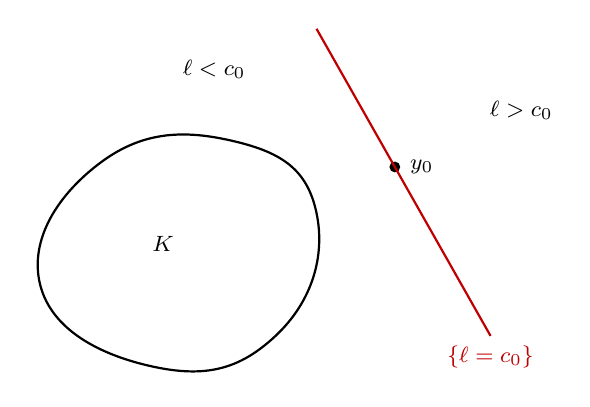
\begin{tikzpicture}[scale=1.3, >=stealth]
    \draw[thick] plot[smooth cycle, tension=0.8] coordinates {(-1.4,-0.3) (-0.8,0.9) (0.5,1.1) (1.3,0.4) (0.9,-0.8) (-0.3,-1.1)};
    \node[font=\footnotesize] at (-0.2,0.1) {$K$};
    \fill (2.065,0.85) circle (1.5pt) node[right, font=\footnotesize, xshift=2pt] {$y_0$};
    \draw[thick, red!75!black] (1.3,2.2) -- (3.0,-0.8) node[below, font=\footnotesize] {$\{\ell = c_0\}$};
    \node[font=\footnotesize] at (0.3,1.8) {$\ell < c_0$};
    \node[font=\footnotesize] at (3.3,1.4) {$\ell > c_0$};
\end{tikzpicture}
\end{center}

\begin{proof}
\textbf{Step 1: Reduction to $0 \in K$.} Assume first that $0 \in K$; the general case is Step 4.

\textbf{Step 2: A functional on a line.} Let $Y = \operatorname{span}\{y_0\} = \{ a y_0 : a \in \mathbb{R} \}$ and define $\ell : Y \to \mathbb{R}$ by
\[
\ell(a y_0) = a, \qquad \text{i.e.\ } \ell(y_0) = 1.
\]
This is a linear functional on $Y$ (the representation $a y_0$ is unique since $y_0 \neq 0$, as $y_0 \notin K \ni 0$).

\textbf{Step 3: Domination by the gauge.} Since $0 \in K$ is an interior point, the gauge $p_K$ is defined, positive homogeneous, and subadditive (Proposition~\ref{prop:gauge-sublinear}). Because every point of $K$ is interior, Corollary~\ref{cor:sublevel} gives
\[
x \in K \iff p_K(x) < 1.
\]
As $y_0 \notin K$, this forces $p_K(y_0) \ge 1$. Hence for $a > 0$, by positive homogeneity,
\[
\ell(a y_0) = a \le a\, p_K(y_0) = p_K(a y_0),
\]
and for $a \le 0$,
\[
\ell(a y_0) = a \le 0 \le p_K(a y_0),
\]
since $p_K \ge 0$. So $\ell \le p_K$ on $Y$. By the Hahn--Banach theorem (Theorem~\ref{thm:hb}), $\ell$ extends to a linear functional $L$ on $X$ with $L(x) \le p_K(x)$ for all $x \in X$. For this $L$,
\[
L(y_0) = \ell(y_0) = 1, \qquad L(x) \le p_K(x) < 1 \quad \text{for all } x \in K,
\]
which is the claim with $c_0 = 1$ and $L$ in the role of the functional in the statement.

\textbf{Step 4: The general case.} (Left to us in lecture; written out here.) If $0 \notin K$, pick any $x_1 \in K$ and translate: $K' = K - x_1 = \{ x - x_1 : x \in K \}$. Translation preserves convexity, sends interior points to interior points (the definition of interior point involves only differences $x_0 + ty$), and sends $x_1$ to $0$, so $K'$ is convex with every point interior and $0 \in K'$; also $y_0 - x_1 \notin K'$. Steps 2--3 give a linear $L : X \to \mathbb{R}$ with $L(y_0 - x_1) = 1$ and $L(x - x_1) < 1$ for all $x \in K$. By linearity, with $c_0 = 1 + L(x_1)$,
\[
L(y_0) = c_0, \qquad L(x) < c_0 \quad \text{for all } x \in K. \qedhere
\]
\end{proof}

\begin{rembox}\label{rem:separation}
Everything in the proof was already in place; the theorem is an assembly. The gauge converts the geometric hypothesis (convex, all points interior, $y_0$ outside) into an inequality $p_K(y_0) \ge 1 = \ell(y_0)$ on a one-dimensional subspace; Hahn--Banach extends $\ell$ without breaking $\ell \le p_K$; and the description $K = \{p_K < 1\}$ converts the inequality back into geometry. The hyperplane is $\{\ell = 1\}$ in the normalized case; there is nothing canonical about it, since the extension is not unique. This is the sense in which a convex set can be described by hyperplanes: it lies on one side of a supporting hyperplane at every point outside it.
\end{rembox}

% ============================================================================
% SECTION 7: COMPLEX HAHN-BANACH
% ============================================================================

\section{The Complex Hahn--Banach Theorem}\label{sec:hb-complex}

\roadmark{Stage: algebra}{Thread: functionals. Reduction to the real case through real parts.}

For a complex linear space the inequality $\ell(y) \le p(y)$ makes no sense, since $\ell(y)$ is complex; the correct hypothesis and conclusion use the modulus, and the homogeneity of $p$ must be strengthened to complex scalars.

\begin{thmbox}[Complex Hahn--Banach]\boxlabel{thm:hb-complex}
Let $X$ be a linear space over $\mathbb{C}$ and $p : X \to \mathbb{R}$ a real-valued function satisfying
\begin{enumerate}[label=(\arabic*)]
    \item $p(ax) = |a|\, p(x)$ for all $a \in \mathbb{C}$, $x \in X$;
    \item $p(x + y) \le p(x) + p(y)$ for all $x, y \in X$.
\end{enumerate}
Let $Y$ be a linear subspace of $X$ and $\ell : Y \to \mathbb{C}$ a linear functional satisfying $|\ell(y)| \le p(y)$ for all $y \in Y$. Then $\ell$ can be extended to a linear functional on $X$ satisfying $|\ell(x)| \le p(x)$ for all $x \in X$.
\laxref{\S3.3, Thm~8}
\end{thmbox}

\begin{lembox}[Consequences of Complex Homogeneity]\boxlabel{lem:p-complex}
Let $p : X \to \mathbb{R}$ satisfy (1) and (2) of Theorem~\ref{thm:hb-complex}. Then $p(0) = 0$, $p(-x) = p(x)$ and $p(x) \ge 0$ for all $x \in X$; and, regarding $X$ as a linear space over $\mathbb{R}$, $p$ is positive homogeneous and subadditive.
\end{lembox}

\begin{proof}
(Not covered in lecture.) (1) with $a = 0$ gives $p(0) = 0$, and with $a = -1$ gives $p(-x) = p(x)$. By (2), $0 = p(x + (-x)) \le p(x) + p(-x) = 2p(x)$. Restricting (1) to real $a \ge 0$ gives positive homogeneity, and (2) is subadditivity.
\end{proof}

\begin{rembox}\label{rem:hb-complex}
The theorem does not assume $p \ge 0$. Wu remarked that $p$ is ``very often'' non-negative; under complex homogeneity it is forced. (Not stated in lecture.)
\end{rembox}

\begin{proof}
As elsewhere, $\ell$ is the given functional on $Y$ and $L$ will be its extension. Two further names are needed because the real theorem is applied to one functional while a different one is being built: $u$ below plays the role of ``$\ell$ on $Y$'' in Theorem~\ref{thm:hb}, and $U$ the role of ``$L$'' there; the complex $L$ is then assembled from $U$. The auxiliary $v$ appears only in Step 2 and is never extended. Regard $X$ also as a linear space over $\mathbb{R}$ (same set, same addition, scalar multiplication restricted to real scalars); $Y$ is then a real subspace. ``Real-linear'' means linear with respect to real scalars; ``complex-linear'' with respect to complex scalars.

\textbf{Step 1: The real part of $\ell$ is real-linear.} Define $u : Y \to \mathbb{R}$ by $u(y) = \operatorname{Re} \ell(y)$. For $y, y' \in Y$ and $c \in \mathbb{R}$,
\[
u(y + y') = \operatorname{Re}\bigl(\ell(y) + \ell(y')\bigr) = u(y) + u(y'), \qquad u(cy) = \operatorname{Re}\bigl(c\,\ell(y)\bigr) = c\, u(y),
\]
the second because $c$ is real. So $u$ is a real-linear functional on $Y$. (The same holds for $\operatorname{Im} \ell$; it will not be needed separately.)

\textbf{Step 2: $\ell$ is determined by $u$.} For $y \in Y$, write $\ell(y) = u(y) + i\,v(y)$ with $v(y) = \operatorname{Im} \ell(y) \in \mathbb{R}$. Since $\ell$ is complex-linear and $iy \in Y$,
\[
\ell(iy) = i\,\ell(y) = i\,u(y) - v(y).
\]
On the other hand, by definition of $u$ and $v$ applied to the vector $iy$,
\[
\ell(iy) = u(iy) + i\,v(iy).
\]
Both right-hand sides are the same complex number; comparing real parts, $u(iy) = -v(y)$. Hence
\begin{equation}\label{eq:complex-recon}
\ell(y) = u(y) - i\,u(iy) \qquad \text{for all } y \in Y.
\end{equation}

\textbf{Step 3: Extend $u$ by the real theorem.} For $y \in Y$,
\[
u(y) = \operatorname{Re} \ell(y) \le |\ell(y)| \le p(y),
\]
since the real part of a complex number is at most its modulus. Also $p$ is positive homogeneous and subadditive on the real space $X$ (Lemma~\ref{lem:p-complex}). So $u$ satisfies the hypotheses of Theorem~\ref{thm:hb} on the real space $X$ with subspace $Y$, and there is a real-linear $U : X \to \mathbb{R}$ with
\[
U|_Y = u \qquad \text{and} \qquad U(x) \le p(x) \quad \text{for all } x \in X.
\]

\textbf{Step 4: Define $L$ and check it is a complex-linear extension.} Guided by \eqref{eq:complex-recon}, define
\[
L : X \to \mathbb{C}, \qquad L(x) = U(x) - i\, U(ix).
\]
This is meaningful since $ix \in X$. Note that $\operatorname{Re} L(x) = U(x)$, as $U$ is real-valued.

\emph{$L$ extends $\ell$.} For $y \in Y$, $iy \in Y$, so $U(y) = u(y)$ and $U(iy) = u(iy)$; then $L(y) = u(y) - i\,u(iy) = \ell(y)$ by \eqref{eq:complex-recon}.

\emph{$L$ is additive and real-homogeneous.} Immediate from real-linearity of $U$ and of $x \mapsto ix$: $L(x + x') = U(x + x') - iU(ix + ix') = L(x) + L(x')$, and $L(cx) = cU(x) - iU(c\,ix) = c\,L(x)$ for $c \in \mathbb{R}$.

\emph{$L(ix) = i\,L(x)$.} Using $i \cdot ix = -x$ and real-linearity of $U$,
\[
L(ix) = U(ix) - i\,U(-x) = U(ix) + i\,U(x) = i\bigl(U(x) - i\,U(ix)\bigr) = i\,L(x).
\]

\emph{Complex homogeneity.} For $c = c_1 + i c_2$ with $c_1, c_2 \in \mathbb{R}$, using the two previous items,
\[
L(cx) = L(c_1 x + c_2\, ix) = c_1 L(x) + c_2 L(ix) = c_1 L(x) + c_2\, i\,L(x) = c\, L(x).
\]
So $L$ is a complex-linear functional on $X$ extending $\ell$.

\textbf{Step 5: The bound $|L(x)| \le p(x)$.} Fix $x \in X$. If $L(x) = 0$ the bound holds since $p \ge 0$ (Lemma~\ref{lem:p-complex}). Otherwise write $L(x) = |L(x)|\,e^{i\theta}$ with $\theta \in [0, 2\pi)$, and set $a = e^{-i\theta} \in \mathbb{C}$, so $|a| = 1$ and
\[
a\,L(x) = |L(x)|.
\]
By complex linearity, $a\,L(x) = L(ax)$. Thus $L(ax)$ is a non-negative real number, so it equals its own real part:
\[
L(ax) = \operatorname{Re} L(ax) = U(ax).
\]
Now apply the bound from Step 3 to the vector $ax$, then homogeneity (1) of $p$:
\[
|L(x)| = L(ax) = U(ax) \le p(ax) = |a|\,p(x) = p(x). \qedhere
\]
\end{proof}

\begin{center}
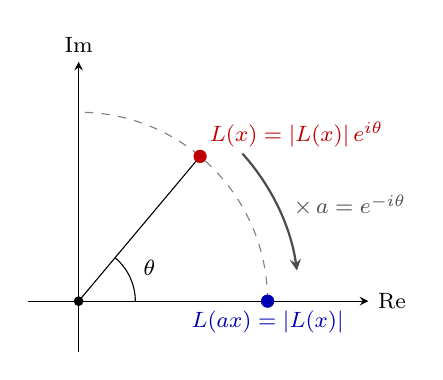
\begin{tikzpicture}[scale=1.6, >=stealth]
    \draw[->] (-0.4,0) -- (2.3,0) node[right] {$\operatorname{Re}$};
    \draw[->] (0,-0.4) -- (0,1.9) node[above] {$\operatorname{Im}$};
    \draw[dashed, gray] (1.5,0) arc (0:90:1.5);
    \coordinate (L) at (50:1.5);
    \draw[thin] (0,0) -- (L);
    \fill[red!75!black] (L) circle (1.5pt) node[above right, red!75!black] {$L(x) = |L(x)|\,e^{i\theta}$};
    \draw (0.45,0) arc (0:50:0.45);
    \node at (25:0.62) {$\theta$};
    \fill[blue!70!black] (1.5,0) circle (1.5pt) node[below, blue!70!black] {$L(ax) = |L(x)|$};
    \draw[->, thick, gray!60!black] (42:1.75) arc (42:8:1.75);
    \node[gray!60!black, anchor=west] at (25:1.8) {$\times\, a = e^{-i\theta}$};
    \fill (0,0) circle (1.1pt);
\end{tikzpicture}
\end{center}
Multiplying $x$ by $a = e^{-i\theta}$ multiplies $L(x)$ by $a$, by complex linearity, rotating it onto the positive real axis. There $L(ax)$ is real, so $L(ax) = U(ax)$, and the real bound $U \le p$ applies.

\begin{rembox}[Why Rotate]\label{rem:why-rotate}
Step 5 is the only place the complex structure does real work. For an arbitrary $x$, $L(x)$ is complex and the real bound $U \le p$ says nothing about its modulus. The trick is to rotate $x$ by the unimodular scalar $a = e^{-i\theta}$, chosen for this one $x$, so that $L(ax)$ becomes real and non-negative; then the real bound applies to $ax$, and homogeneity of $p$ with $|a| = 1$ undoes the rotation on the right-hand side. A student proposed instead the direct route $|L(x)|^2 = U(x)^2 + U(ix)^2 \le p(x)^2 + p(ix)^2 = 2p(x)^2$; this gives only $|L(x)| \le \sqrt{2}\,p(x)$, which is too weak (and even that needs $U \ge -p$, i.e.\ $|U| \le p$, which follows from $U(-x) \le p(-x) = p(x)$). The rotation gets the constant $1$ because it uses the bound once, on a single well-chosen vector, rather than twice.
\end{rembox}


% Lecture 2 was cut short by a tornado warning during a second gauge example
% (a non-standard convex set K with vertices at (+-2,0), (0,+-2) drawn on the board).
% That example was not completed and is omitted here; to be picked up next lecture.


% ============================================================================
% CHAPTER 3: NORMED LINEAR SPACES
% ============================================================================
% Lecture 4 (2026-09-10). Wu's board order: norm -> metric -> convergence/Cauchy ->
% completion -> complete/Banach -> equivalent norms -> subspace/direct sum norms ->
% quotient norm -> completion norm (HW) -> Holder. Reordered here so that
% "complete" precedes "completion".

\chapter{Normed Linear Spaces}

So far $X$ has had only linear structure, and the Hahn--Banach theorem is the most one can say. The next layer of structure is a notion of length. With it come distance, convergence, Cauchy sequences, and completeness, and the objects of the course (Banach spaces) can finally be defined. This lecture follows Lax's book.

\begin{notebox}[Notation]\label{note:notation-4}
Wu writes norms as $|x|$ on the board. These notes use $\|x\|$, reserving $|\cdot|$ for the modulus of a scalar; the two appear side by side in the homogeneity axiom.
\end{notebox}

\section{Normed Linear Spaces}\label{sec:normed}

\roadmark{Stage: norms}{Thread: convexity. A norm is a symmetric gauge (Proposition~\ref{prop:norm-gauge}); with it come distance, convergence and closed sets.}

\subsection{Definition and Examples}

\begin{defbox}[Norm; Normed Linear Space]\boxlabel{def:norm}
Let $X$ be a linear space over $\mathbb{F}$ ($= \mathbb{R}$ or $\mathbb{C}$). A function $\|\cdot\| : X \to \mathbb{R}_+ = \{a \in \mathbb{R} : a \ge 0\}$ is a \textbf{norm} if
\begin{enumerate}[label=(\arabic*)]
    \item \textbf{positivity}: $\|x\| \ge 0$ for all $x \in X$, and $\|x\| = 0$ if and only if $x = 0$;
    \item \textbf{homogeneity}: $\|ax\| = |a|\, \|x\|$ for all $a \in \mathbb{F}$, $x \in X$;
    \item \textbf{subadditivity} (triangle inequality): $\|x + y\| \le \|x\| + \|y\|$ for all $x, y \in X$.
\end{enumerate}
The pair $(X, \|\cdot\|)$ is a \textbf{normed linear space}. When the norm is understood one writes simply $X$.
\laxref{\S5.1, (1)--(3)}
\end{defbox}

\begin{defbox}[Seminorm]\boxlabel{def:seminorm}
A function $q : X \to \mathbb{R}_+$ on a linear space $X$ over $\mathbb{F}$ is a \textbf{seminorm} if it satisfies homogeneity and subadditivity, (2) and (3) of Definition~\ref{def:norm}, but not necessarily positivity: $q(x) = 0$ is allowed for some $x \neq 0$.
\end{defbox}

\begin{propbox}[Norms and Gauges]\boxlabel{prop:norm-gauge}
Let $X$ be a linear space over $\mathbb{R}$.
\begin{enumerate}[label=(\alph*)]
    \item Every norm on $X$ is positive homogeneous and subadditive.
    \item If $\|\cdot\|$ is a norm on $X$ and $K = \{ x : \|x\| < 1 \}$ or $K = \{ x : \|x\| \le 1 \}$, then $K$ is convex, $0$ is an interior point of $K$, and $p_K = \|\cdot\|$.
    \item Conversely, let $K$ be convex with $0$ an interior point. Then $p_K$ is a norm if and only if $K$ contains no full ray (for every $x \neq 0$ there is $s > 0$ with $sx \notin K$) and $p_K(-x) = p_K(x)$ for all $x$. The last condition holds in particular when $K = -K$.
\end{enumerate}
\end{propbox}

\begin{proof}
(Not covered in lecture.) (a) Positive homogeneity is homogeneity restricted to $a \ge 0$; subadditivity is an axiom.

(b) $K$ is convex by Proposition~\ref{prop:sublevel-convex} with $p = \|\cdot\|$. Given $y \in X$, put $\varepsilon(y) = 1/(\|y\| + 1)$; for $|t| < \varepsilon(y)$, $\|ty\| = |t|\,\|y\| < 1$, so $ty \in K$, and $0$ is an interior point. For $a > 0$, $x/a \in K$ iff $\|x\| < a$ (respectively $\|x\| \le a$), so $A(x) = (\|x\|, \infty)$ (respectively $[\|x\|, \infty)$), and in either case $p_K(x) = \inf A(x) = \|x\|$.

(c) By Propositions~\ref{prop:gauge-sublinear} and~\ref{prop:gauge-values}(a), $p_K$ is non-negative, positive homogeneous and subadditive, and by Proposition~\ref{prop:gauge-values}(c), $p_K(x) = 0$ iff the ray $\{sx : s \ge 0\}$ lies in $K$; so $p_K$ satisfies positivity iff $K$ contains no full ray. If moreover $p_K(-x) = p_K(x)$, then for $a < 0$, $p_K(ax) = p_K(|a|(-x)) = |a|\,p_K(-x) = |a|\,p_K(x)$, which with positive homogeneity gives homogeneity for all real $a$, and $p_K$ is a norm. Conversely a norm satisfies positivity and $\|{-x}\| = \|x\|$. Finally, if $K = -K$ then $x/a \in K$ iff $-x/a \in K$, so $A(-x) = A(x)$ and $p_K(-x) = p_K(x)$.
\end{proof}

\begin{rembox}[Relation to the Functions $p$ of Chapter 2]\label{rem:relation-functions-p-chapter-2}
By (a), every Hahn--Banach statement applies with $p = \|\cdot\|$ or $p = C\|\cdot\|$. The converse of (a) is false, and not only because a positive homogeneous subadditive $p$ may take negative values: even a non-negative one with $p(x) = 0 \Rightarrow x = 0$ need not be a norm, since nothing forces $p(-x) = p(x)$. On $\mathbb{R}$, $p(x) = \max\{x, 0\} + 2\max\{-x, 0\}$ is such a function, with $p(1) = 1 \neq 2 = p(-1)$. By (b) and (c), norms on a real space correspond to convex sets with $0$ interior that contain no full ray and are symmetric; the unit ball is the geometric picture of the norm, as with the disk, square and diamond of Example~\ref{ex:p-sets}.
\end{rembox}

\begin{exbox}[Norms on $\mathbb{R}^n$]\boxlabel{ex:norms-rn}
On $X = \mathbb{R}^n$, the following are norms:
\begin{align*}
\|x\|_2 &= \bigl(x_1^2 + \cdots + x_n^2\bigr)^{1/2} && \text{(Euclidean, or $\ell^2$, norm)} \\
\|x\|_\infty &= \max_{1 \le i \le n} |x_i| && \text{($\ell^\infty$, or maximum, norm)} \\
\|x\|_1 &= |x_1| + \cdots + |x_n| && \text{($\ell^1$ norm)} \\
\|x\|_p &= \Bigl( \sum_{i=1}^n |x_i|^p \Bigr)^{1/p}, \quad 1 \le p < \infty && \text{($\ell^p$ norm).}
\end{align*}
For $\|\cdot\|_2$, $\|\cdot\|_\infty$, $\|\cdot\|_1$ the axioms were checked in Example~\ref{ex:three-p} (as $p_1, p_2, p_3$; positivity is immediate). That $\|\cdot\|_p$ is subadditive for general $p$ is Minkowski's inequality, proved in Chapter~4; the other axioms are immediate. Thus one linear space carries many norms, and $\mathbb{R}^n$ alone is not enough to see what a norm can do; the point of the definition is infinite-dimensional spaces.
\laxref{\S5.1, examples (a)--(b), for sequences}
\end{exbox}

\subsection{The Induced Metric}

\begin{defbox}[Metric Space]\boxlabel{def:metric-space}
A \textbf{metric} on a set $M$ is a function $d : M \times M \to \mathbb{R}$ such that for all $x, y, z \in M$:
\begin{enumerate}[label=(\roman*)]
    \item $d(x, y) \ge 0$, and $d(x, y) = 0$ if and only if $x = y$;
    \item $d(x, y) = d(y, x)$;
    \item $d(x, y) \le d(x, z) + d(z, y)$.
\end{enumerate}
$(M, d)$ is a \textbf{metric space}. A metric space need not be a linear space.
\end{defbox}

\begin{propbox}[A Normed Space is a Metric Space]\boxlabel{prop:norm-metric}
Let $(X, \|\cdot\|)$ be a normed linear space and define $d(x, y) = \|x - y\|$ for $x, y \in X$. Then $(X, d)$ is a metric space.
\laxref{\S5.1, (4)}
\end{propbox}

\begin{proof}
(Stated without proof in lecture; the check is routine.) (i) $d(x,y) = \|x - y\| \ge 0$, and it is $0$ iff $x - y = 0$ iff $x = y$, by positivity. (ii) $d(y, x) = \|y - x\| = \|(-1)(x - y)\| = |{-1}|\, \|x - y\| = d(x, y)$, by homogeneity with $a = -1$; a student asked whether symmetry is automatic, and this is why it is. (iii) $d(x, y) = \|(x - z) + (z - y)\| \le \|x - z\| + \|z - y\| = d(x, z) + d(z, y)$, by subadditivity.
\end{proof}

The metric is translation invariant, $d(x + z, y + z) = d(x, y)$, and homogeneous, $d(ax, ay) = |a|\,d(x,y)$; a general metric on a linear space need not be either. Everything available in a metric space --- limits, open and closed sets, continuity --- is now available in $X$.

\subsection{Convergence and Cauchy Sequences}

\begin{defbox}[Convergence]\boxlabel{def:convergence}
Let $X$ be a normed linear space. A sequence $\{x_n\}_{n=1}^\infty \subset X$ \textbf{converges} to $x_0 \in X$, written $x_n \to x_0$, if
\[
\lim_{n \to \infty} \|x_n - x_0\| = 0.
\]
\end{defbox}

\begin{lembox}[Reverse Triangle Inequality]\boxlabel{lem:reverse-triangle}
For all $x, y$ in a normed linear space $X$,
\[
\bigl|\, \|x\| - \|y\| \,\bigr| \;\le\; \|x - y\|.
\]
\end{lembox}

\begin{proof}
By subadditivity applied to $x = (x - y) + y$,
\[
\|x\| \le \|x - y\| + \|y\|, \qquad \text{i.e.} \qquad \|x\| - \|y\| \le \|x - y\|.
\]
Exchanging $x$ and $y$ and using $\|y - x\| = \|x - y\|$ (homogeneity with $a = -1$),
\[
\|y\| - \|x\| \le \|x - y\|.
\]
The two together bound the absolute value.
\end{proof}

\begin{propbox}[A Norm is Continuous]\boxlabel{prop:norm-continuous}
Let $(X, \|\cdot\|)$ be a normed linear space. Then $\|\cdot\| : X \to \mathbb{R}$ is uniformly continuous: for every $\varepsilon > 0$ there is $\delta > 0$ --- indeed $\delta = \varepsilon$ works --- such that
\[
\|x - y\| < \delta \implies \bigl|\, \|x\| - \|y\| \,\bigr| < \varepsilon \qquad \text{for all } x, y \in X.
\]
In particular, if $x_n \to x_0$ in $X$ then $\|x_n\| \to \|x_0\|$ in $\mathbb{R}$.
\end{propbox}

\begin{proof}
Given $\varepsilon > 0$ take $\delta = \varepsilon$. If $\|x - y\| < \delta$ then by Lemma~\ref{lem:reverse-triangle}, $\bigl|\|x\| - \|y\|\bigr| \le \|x - y\| < \varepsilon$. The $\delta$ does not depend on $x$ or $y$, so the continuity is uniform; the constant $1$ in the lemma says $\|\cdot\|$ is Lipschitz. For the last claim apply this with $y = x_0$ and $x = x_n$.
\end{proof}

\begin{rembox}[What This Does and Does Not Say]\label{rem:what-this-does-does-not-say}
The statement is not circular, although it can sound so. It compares two metric spaces: $X$ with $d(x,y) = \|x - y\|$, and $\mathbb{R}$ with $|s - t|$; neither metric is defined in terms of the continuity being asserted. Only subadditivity and homogeneity are used --- positivity is not --- so the same proof shows any seminorm, and any positive homogeneous subadditive $p$ that happens to satisfy $p(-x) = p(x)$, is $1$-Lipschitz.

The question has content whenever a second topology is present. Whether a norm $\|\cdot\|_1$ is continuous with respect to another norm $\|\cdot\|_2$ is settled by Proposition~\ref{prop:norm-cont-other}: exactly when $\|x\|_1 \le C\|x\|_2$ for some constant $C$, which is one half of equivalence of the two norms; on $\mathbb{R}^n$ this always holds, in infinite dimensions it need not. Later in the course $X$ will also carry the weak topology, in which the norm is \emph{not} continuous. (Not covered in lecture.)
\end{rembox}

\begin{defbox}[Cauchy Sequence]\boxlabel{def:cauchy-sequence}
A sequence $\{x_n\} \subset X$ is \textbf{Cauchy} if for every $\varepsilon > 0$ there is $N = N(\varepsilon) \in \mathbb{N}$ such that
\[
\|x_m - x_k\| < \varepsilon \qquad \text{for all } m, k \ge N.
\]
\end{defbox}

\begin{propbox}[Limits are Unique; Convergent Sequences are Cauchy]\boxlabel{prop:conv-basic}
Let $\{x_n\}$ be a sequence in a normed linear space $X$.
\begin{enumerate}[label=(\alph*)]
    \item If $x_n \to x$ and $x_n \to x'$, then $x = x'$.
    \item If $x_n \to x$, then $\{x_n\}$ is Cauchy.
\end{enumerate}
\end{propbox}

\begin{proof}
(Not covered in lecture.) (a) $\|x - x'\| \le \|x - x_n\| + \|x_n - x'\| \to 0$, so $\|x - x'\| = 0$ and $x = x'$ by positivity. (b) Given $\varepsilon > 0$, choose $N$ with $\|x_n - x\| < \varepsilon/2$ for $n \ge N$; then for $m, k \ge N$, $\|x_m - x_k\| \le \|x_m - x\| + \|x - x_k\| < \varepsilon$.
\end{proof}

\begin{rembox}\label{rem:normed}
Convergence refers to a limit \emph{in $X$}; a Cauchy sequence has its terms approaching one another with no limit mentioned. The converse of (b) fails: a Cauchy sequence may fail to converge because the point it is heading toward is missing from $X$ --- the standard example being a sequence of rationals approaching $\sqrt{2}$ inside $\mathbb{Q}$. Spaces without this defect are the subject of the next section. Both statements, and their proofs, hold verbatim in any metric space.
\end{rembox}

\begin{defbox}[Closed Subset]\boxlabel{def:closed}
A subset $S$ of a normed linear space (or metric space) $X$ is \textbf{closed} if it contains the limits of all its convergent sequences: whenever $\{s_n\} \subset S$ and $s_n \to x$ with $x \in X$, then $x \in S$.
\end{defbox}

\begin{defbox}[Closure; Dense Subset]\boxlabel{def:closure}
Let $S$ be a subset of a normed linear space (or metric space) $X$. The \textbf{closure} $\overline{S}$ of $S$ is the set of all limits of convergent sequences in $S$:
\[
\overline{S} = \{ x \in X : x = \lim_{n \to \infty} s_n \text{ for some sequence } s_n \in S \} .
\]
$S$ is \textbf{dense} in $X$ if $\overline{S} = X$.
\laxref{\S5.1, before Thm~2; ``dense'' in the definition of separable space}
\end{defbox}

\begin{propbox}[Properties of the Closure]\boxlabel{prop:closure}
Let $S$ be a subset of a normed linear space $X$.
\begin{enumerate}[label=(\alph*)]
    \item $S \subset \overline{S}$, and $\overline{S}$ is closed.
    \item $S$ is closed if and only if $S = \overline{S}$.
    \item If $T$ is closed and $S \subset T$, then $\overline{S} \subset T$; so $\overline{S}$ is the smallest closed set containing $S$.
    \item If $S$ is a linear subspace, so is $\overline{S}$.
\end{enumerate}
\laxref{\S5.1, Thm~2 (part (d))}
\end{propbox}

\begin{proof}
(Not covered in lecture.) (a) $s \in S$ is the limit of the constant sequence $s, s, \ldots$. Let $x_k \in \overline{S}$ with $x_k \to x$. For each $k$ choose $s_k \in S$ with $\|s_k - x_k\| < 1/k$; then $\|s_k - x\| \le 1/k + \|x_k - x\| \to 0$, so $x \in \overline{S}$.

(b) By Definition~\ref{def:closed}, $S$ is closed iff every limit of a sequence in $S$ lies in $S$, i.e.\ iff $\overline{S} \subset S$; with (a), iff $\overline{S} = S$.

(c) A limit of a sequence in $S$ is a limit of a sequence in $T$, hence lies in $T$ since $T$ is closed.

(d) $0 \in S \subset \overline{S}$. If $s_n \to x$ and $t_n \to y$ with $s_n, t_n \in S$, and $a, b \in \mathbb{F}$, then $a s_n + b t_n \in S$ and
\[
\|(a s_n + b t_n) - (ax + by)\| \le |a|\,\|s_n - x\| + |b|\,\|t_n - y\| \to 0,
\]
so $ax + by \in \overline{S}$.
\end{proof}

\begin{defbox}[Closed Linear Span]\boxlabel{def:closed-span}
The \textbf{closed linear span} of a subset $S$ of a normed linear space $X$ is $\overline{\operatorname{span}}\, S := \overline{\operatorname{span} S}$. By Proposition~\ref{prop:closure}(a),(c),(d), it is a closed linear subspace of $X$, and it is the smallest closed linear subspace containing $S$.
\laxref{\S6.4, closed linear span}
\end{defbox}

\begin{defbox}[Open Ball; Metric Interior Point]\boxlabel{def:metric-interior}
For $x_0 \in X$ and $r > 0$, the \textbf{open ball} of radius $r$ about $x_0$ is $B_r(x_0) = \{ x \in X : \|x - x_0\| < r \}$. A point $x_0$ of a subset $K \subset X$ is a \textbf{metric interior point} of $K$ if $B_r(x_0) \subset K$ for some $r > 0$.
\end{defbox}

\begin{propbox}[Metric Interior Points are Interior Points]\boxlabel{prop:metric-interior}
Let $K$ be a subset of a normed linear space $X$. Every metric interior point of $K$ is an interior point of $K$ in the sense of Definition~\ref{def:interior}.
\end{propbox}

\begin{proof}
Let $B_r(x_0) \subset K$ and $y \in X$. If $y = 0$, then $x_0 + ty = x_0 \in K$ for all $t$. If $y \neq 0$, put $\varepsilon(y) = r/\|y\|$; for $|t| < \varepsilon(y)$, $\|(x_0 + ty) - x_0\| = |t|\,\|y\| < r$, so $x_0 + ty \in B_r(x_0) \subset K$. (Not covered in lecture.)
\end{proof}

\begin{exbox}[An Interior Point that is Not a Metric Interior Point]\boxlabel{ex:interior-point-not-metric-interior-point}
In $\mathbb{R}^2$ with the Euclidean norm, let $P = \{ (s, s^2) : s \neq 0 \}$ and $K = \mathbb{R}^2 \setminus P$. Then $0 \in K$ is an interior point of $K$ but not a metric interior point.

\emph{Not metric interior.} $(1/n, 1/n^2) \in P$, so $(1/n, 1/n^2) \notin K$, while $\|(1/n, 1/n^2)\| \to 0$; so no ball $B_r(0)$ lies in $K$.

\emph{Interior.} For $y = 0$ there is nothing to check. Let $y = (y_1, y_2) \neq 0$. A point $ty$ lies in $P$ iff $t y_1 = s$ and $t y_2 = s^2$ for some $s \neq 0$, which forces $t \neq 0$, $y_1 \neq 0$ and $y_2 = t y_1^2$, i.e.\ $t = y_2 / y_1^2$. So the line $\{ty : t \in \mathbb{R}\}$ meets $P$ in at most one point, at a parameter $t^* \neq 0$, and $\varepsilon(y) = |t^*|$ works (any $\varepsilon(y)$ works if the line misses $P$).

The definition of interior point tests one line at a time, and the parabola approaches $0$ along no single line. The set $K$ is not convex.
\end{exbox}

% ============================================================================
% SECTION 9: COMPLETENESS
% ============================================================================

\section{Completeness}\label{sec:completeness}

\roadmark{Stage: norms}{Thread: completeness. Cauchy sequences, Banach spaces, and the completion.}

\subsection{Complete Spaces and Banach Spaces}

\begin{defbox}[Complete Metric Space]\boxlabel{def:complete-metric-space}
A metric space $(M, d)$ is \textbf{complete} if every Cauchy sequence in $M$ converges to a point of $M$.
\end{defbox}

\begin{defbox}[Banach Space]\boxlabel{def:banach-space}
A complete normed linear space is called a \textbf{Banach space}.
\laxref{\S5.1, definition of Banach space}
\end{defbox}

\begin{thmbox}[{{$C[a,b]$ with the Supremum Norm is a Banach Space}}]\boxlabel{thm:Cab-banach}
Let $X = C([a,b])$ be the set of continuous functions $f : [a,b] \to \mathbb{F}$, with pointwise operations and
\[
\|f\|_\infty = \max_{t \in [a,b]} |f(t)|.
\]
Then $(X, \|\cdot\|_\infty)$ is a Banach space.
\laxref{\S5.1, examples (c)--(e)}
\end{thmbox}

\begin{proof}
(HW2, Problem 1.) Throughout, $\mathbb{F}$ denotes the scalar field, $\mathbb{R}$ or $\mathbb{C}$, and $|\cdot|$ its absolute value. We show in turn that $X$ is a linear space, that $\|\cdot\|_\infty$ is a norm on $X$, and that $(X, \|\cdot\|_\infty)$ is complete.

\textbf{Part 1: $X$ is a linear space.} Define addition and scalar multiplication pointwise: for $f, g \in X$ and $a \in \mathbb{F}$,
\[
(f + g)(x) = f(x) + g(x), \qquad (af)(x) = a\,f(x) \qquad (x \in [a,b]).
\]
These are well defined as operations on $X$: a sum of continuous functions is continuous and a scalar multiple of a continuous function is continuous, so $f + g \in X$ and $af \in X$. Let $f, g, h \in X$ and $a, k \in \mathbb{F}$; each identity below is proved by evaluating at an arbitrary $x \in [a,b]$, where it reduces to the corresponding identity in $\mathbb{F}$.

\emph{Commutativity:} $(f + g)(x) = f(x) + g(x) = g(x) + f(x) = (g + f)(x)$, so $f + g = g + f$.

\emph{Associativity:} $\bigl((f + g) + h\bigr)(x) = \bigl(f(x) + g(x)\bigr) + h(x) = f(x) + \bigl(g(x) + h(x)\bigr) = \bigl(f + (g + h)\bigr)(x)$.

\emph{Additive identity:} the constant function $Z(x) = 0$ is continuous, so $Z \in X$, and $(f + Z)(x) = f(x) + 0 = f(x) = 0 + f(x) = (Z + f)(x)$.

\emph{Additive inverse:} $(-f)(x) = -f(x)$ defines $-f \in X$, and $\bigl(f + (-f)\bigr)(x) = f(x) - f(x) = 0 = Z(x) = -f(x) + f(x) = \bigl((-f) + f\bigr)(x)$.

\emph{Compatibility of scalar multiplication:} $\bigl(k(af)\bigr)(x) = k\bigl(a f(x)\bigr) = (ka) f(x) = \bigl((ka)f\bigr)(x)$.

\emph{Distributivity over vector addition:} $\bigl(k(f + g)\bigr)(x) = k\bigl(f(x) + g(x)\bigr) = k f(x) + k g(x) = (kf + kg)(x)$.

\emph{Distributivity over scalar addition:} $\bigl((a + k)f\bigr)(x) = (a + k)f(x) = a f(x) + k f(x) = (af + kf)(x)$.

\emph{Unit:} $(1f)(x) = 1 \cdot f(x) = f(x)$.

Hence $X$ is a linear space over $\mathbb{F}$.

\textbf{Part 2: $\|\cdot\|_\infty$ is a norm on $X$.}

\emph{The maximum is attained.} Let $f \in X$. Since $f$ and $|\cdot|$ are continuous, $|f| : [a,b] \to \mathbb{R}$ is continuous, and a continuous real-valued function on the closed bounded interval $[a,b]$ attains its maximum. Hence there is $t_0 \in [a,b]$ with $|f(t_0)| \ge |f(t)|$ for all $t$, so $\|f\|_\infty = |f(t_0)|$ is a well-defined real number, and $|f(t)| \le \|f\|_\infty$ for every $t \in [a,b]$.

\emph{Positivity.} Since $|f(t)| \ge 0$ for every $t$, $\|f\|_\infty \ge 0$. If $\|f\|_\infty = 0$, then $0 \le |f(t)| \le \|f\|_\infty = 0$ for every $t$, so $f(t) = 0 = Z(t)$; hence $f = Z$.

\emph{Homogeneity.} Let $k \in \mathbb{F}$ and let $t_0$ be as above for $f$. For every $t$, $|(kf)(t)| = |k|\,|f(t)| \le |k|\,|f(t_0)| = |(kf)(t_0)|$, so the maximum of $|kf|$ is attained at $t_0$ as well, and $\|kf\|_\infty = |k|\,|f(t_0)| = |k|\,\|f\|_\infty$.

\emph{Triangle inequality.} Let $t_0$ be a point where $|f + g|$ attains its maximum. Then
\[
\|f + g\|_\infty = |f(t_0) + g(t_0)| \le |f(t_0)| + |g(t_0)| \le \|f\|_\infty + \|g\|_\infty,
\]
the first inequality being the triangle inequality in $\mathbb{F}$ and the second the bound $|f(t)| \le \|f\|_\infty$, $|g(t)| \le \|g\|_\infty$.

\textbf{Part 3: completeness.} Let $\{f_n\}$ be Cauchy in $X$: for every $\varepsilon > 0$ there is $N$ with $\|f_m - f_k\|_\infty < \varepsilon$ for all $m, k \ge N$. We must produce $f \in X$ with $\|f_n - f\|_\infty \to 0$.

\emph{Step 1: pointwise convergence.} Fix $t_0 \in [a,b]$. For all $m, k$,
\[
0 \le |f_m(t_0) - f_k(t_0)| = |(f_m - f_k)(t_0)| \le \|f_m - f_k\|_\infty .
\]
So $\{f_n(t_0)\}$ is a Cauchy sequence of scalars; as $\mathbb{F}$ is complete, it converges. Define $f(t_0) = \lim_n f_n(t_0)$. Doing this for every $t_0$ defines $f : [a,b] \to \mathbb{F}$ with $f_n(t) \to f(t)$ for each $t$.

\emph{Step 2: the convergence is uniform.} Let $\varepsilon > 0$ and choose $N$ with
\[
|f_m(t) - f_k(t)| \le \|f_m - f_k\|_\infty < \frac{\varepsilon}{2} \qquad \text{for all } m, k > N \text{ and all } t \in [a,b];
\]
$N$ was obtained from the norm estimate alone, so it does not depend on $t$. Fix $k > N$ and $t \in [a,b]$, and consider $S_m(t) = |f_m(t) - f_k(t)|$ for $m > N$; each is at most $\varepsilon/2$. By the reverse triangle inequality in $\mathbb{F}$,
\[
\Bigl|\, |f_m(t) - f_k(t)| - |f(t) - f_k(t)| \,\Bigr| \le |f_m(t) - f(t)| \xrightarrow[m \to \infty]{} 0,
\]
so $S_m(t) \to |f(t) - f_k(t)|$. A limit preserves non-strict inequalities, so $|f(t) - f_k(t)| \le \varepsilon/2 < \varepsilon$. Here $N$ was chosen before $t$ and $k > N$ was arbitrary: for every $\varepsilon > 0$ there is $N$, independent of $t$, with $|f_k(t) - f(t)| < \varepsilon$ for all $k > N$ and all $t$. That is, $f_n \to f$ uniformly on $[a,b]$.

\emph{Step 3: $f$ is continuous.} Fix $x \in [a,b]$ and $\varepsilon > 0$. By Step 2 there is $N$, independent of the point, with $|f_n(t) - f(t)| < \varepsilon/3$ for all $n > N$ and all $t$. Fix one such $n$. Since $f_n$ is continuous at $x$, there is $\delta > 0$ with $|f_n(x) - f_n(y)| < \varepsilon/3$ whenever $|x - y| < \delta$. For such $y$,
\begin{align*}
|f(x) - f(y)| &\le |f(x) - f_n(x)| + |f_n(x) - f_n(y)| + |f_n(y) - f(y)| < \frac{\varepsilon}{3} + \frac{\varepsilon}{3} + \frac{\varepsilon}{3} = \varepsilon,
\end{align*}
the first and third terms bounded at the two points $x$ and $y$ with the \emph{same} index $n$, which is legitimate because $N$ does not depend on the point. Hence $f$ is continuous at every $x$, i.e.\ $f \in X$.

\emph{Step 4: $\|f_n - f\|_\infty \to 0$.} Let $\varepsilon > 0$ and $N$ as in Step 2, so $|f_m(t) - f(t)| < \varepsilon$ for all $m > N$ and all $t$. Fix $m > N$. By Step 3, $f_m - f \in X$, so by Part 2 its modulus attains a maximum at some $t_0$, and
\[
\|f_m - f\|_\infty = |f_m(t_0) - f(t_0)| < \varepsilon .
\]
Hence $\|f_n - f\|_\infty \to 0$, and every Cauchy sequence in $X$ converges in $X$. With Parts 1 and 2, $(X, \|\cdot\|_\infty)$ is a Banach space.
\end{proof}

\begin{rembox}\label{rem:completeness}
The proof is the ``candidate, then close'' pattern (Technique~5) in its simplest form, with one extra step that has no analogue in $\ell^p$: the candidate must be shown to lie in the space, and here that is a genuine theorem (a uniform limit of continuous functions is continuous), not a bookkeeping check. The $3\varepsilon$ argument in Step 3 is exactly where uniformity, not just pointwise convergence, is used.
\end{rembox}

\begin{rembox}\label{rem:completeness-2}
The hierarchy so far: a linear space has only algebra; a normed linear space adds length and hence topology; a Banach space adds the guarantee that limits exist. Most of the course is about Banach spaces, because that is where analysis --- limits of sequences, sums of series, solutions of equations obtained as limits of approximations --- can actually be carried out.
\end{rembox}

\begin{lembox}[Complete Subsets are Closed]\boxlabel{lem:complete-closed}
Let $S$ be a subset of a normed linear space (or metric space) $X$ which is complete with the restricted norm (metric). Then $S$ is closed in $X$.
\end{lembox}

\begin{proof}
(Not covered in lecture.) Let $s_n \in S$ with $s_n \to x \in X$. By Proposition~\ref{prop:conv-basic}(b), $\{s_n\}$ is Cauchy, so by completeness of $S$ it converges to some $s \in S$. By uniqueness of limits (Proposition~\ref{prop:conv-basic}(a)), $x = s \in S$.
\end{proof}

\subsection{Completion of a Metric Space}

A metric space that is not complete can be enlarged to one that is, by adjoining the missing limits. Since a missing limit is not an element of $M$, it is represented by the Cauchy sequences that ``should'' converge to it.

\begin{defbox}[Equivalent Cauchy Sequences]\boxlabel{def:equivalent-cauchy-sequences}
Two Cauchy sequences $\{x_n\}, \{y_n\}$ in a metric space $(M, d)$ are \textbf{equivalent}, written $\{x_n\} \sim \{y_n\}$, if
\[
\lim_{n \to \infty} d(x_n, y_n) = 0.
\]
\end{defbox}

Note that $d(x_n, y_n)$ makes sense whether or not either sequence has a limit in $M$: both terms lie in $M$. The relation says the two sequences are heading for the same place. If one of them converges in $M$, so does the other, to the same limit.

\begin{defbox}[Completion]\boxlabel{def:completion}
The \textbf{completion} $\overline{M}$ of a metric space $M$ is the set of equivalence classes of Cauchy sequences in $M$ under $\sim$:
\[
\overline{M} = \bigl\{ [\{x_n\}] : \{x_n\} \text{ Cauchy in } M \bigr\}.
\]
An element $x \in M$ is identified with the class of the constant sequence $(x, x, x, \ldots)$, which is Cauchy with limit $x$; in this way $M \subset \overline{M}$.
\laxref{\S5.1, completion of a metric space}
\end{defbox}

\begin{rembox}[{{Why Classes, and Why the Objects Look Different}}]\label{rem:why-classes-why-objects-look-different}
Two points were raised in lecture. First, why equivalence classes: a point $x \in M$ is the limit of many Cauchy sequences (on the real line, $(x, x, \ldots)$ and $(x + 1/n)$ both converge to $x$), and different sequences with the same destination must not be counted as different elements of $\overline{M}$. Second, the elements of $\overline{M}$ are sets of sequences, not points of $M$, so how is $M$ a subset? By the identification $x \leftrightarrow [(x, x, \ldots)]$, which is one-to-one; $M$ is not literally contained in $\overline{M}$ but is embedded in it. This is the same kind of identification as $\mathbb{R} \subset \mathbb{R} \oplus \mathbb{R}^2 = \mathbb{R}^3$.
\end{rembox}

\begin{propbox}[{{The Completion is a Complete Metric Space, and $M$ is Dense in It}}]\boxlabel{prop:completion-metric}
Let $(M, d)$ be a metric space. For Cauchy sequences $\{x_n\}, \{y_n\}$ in $M$ put
\[
\bar d\bigl([\{x_n\}], [\{y_n\}]\bigr) := \lim_{n \to \infty} d(x_n, y_n).
\]
\begin{enumerate}[label=(\alph*)]
    \item The limit exists and depends only on the classes, and $\bar d$ is a metric on $\overline{M}$.
    \item $\bar d(x, y) = d(x, y)$ for $x, y \in M$ (identified with constant sequences), so $M \subset \overline{M}$ isometrically.
    \item $M$ is dense in $\overline{M}$: if $\xi = [\{x_n\}]$, then $x_k \to \xi$ in $\overline{M}$ as $k \to \infty$.
    \item $(\overline{M}, \bar d)$ is complete.
\end{enumerate}
\end{propbox}

\begin{proof}
(Not covered in lecture; added because Example~\ref{ex:completions-subsets-rn}, Remark~\ref{rem:how-do-we-know-we-have-not-added-too-much} and the normed case below rely on these facts.)

(a) By the triangle inequality, applied twice, $|d(x_n, y_n) - d(x_m, y_m)| \le d(x_n, x_m) + d(y_n, y_m)$, so $\{d(x_n, y_n)\}$ is a Cauchy sequence of real numbers and converges. If $\{x_n\} \sim \{x_n'\}$ and $\{y_n\} \sim \{y_n'\}$, the same estimate gives $|d(x_n, y_n) - d(x_n', y_n')| \le d(x_n, x_n') + d(y_n, y_n') \to 0$, so the limit depends only on the classes. Symmetry and the triangle inequality hold termwise and pass to the limit, and $\bar d \ge 0$. Finally $\bar d([\{x_n\}], [\{y_n\}]) = 0$ iff $d(x_n, y_n) \to 0$ iff $\{x_n\} \sim \{y_n\}$ iff the two classes are equal.

(b) For constant sequences, $\bar d(x, y) = \lim_n d(x, y) = d(x, y)$.

(c) Let $\varepsilon > 0$ and choose $N$ with $d(x_n, x_m) < \varepsilon$ for all $n, m \ge N$. For $k \ge N$, $\bar d(x_k, \xi) = \lim_n d(x_k, x_n) \le \varepsilon$. Hence $x_k \to \xi$.

(d) Let $\{\xi_m\}$ be a Cauchy sequence in $\overline{M}$. By (c) there are $z_m \in M$ with $\bar d(z_m, \xi_m) < 1/m$. By (b) and the triangle inequality,
\[
d(z_m, z_k) = \bar d(z_m, z_k) \le \frac{1}{m} + \bar d(\xi_m, \xi_k) + \frac{1}{k},
\]
so $\{z_m\}$ is Cauchy in $M$; let $\xi = [\{z_m\}] \in \overline{M}$. Then $\bar d(\xi_m, \xi) \le 1/m + \bar d(z_m, \xi)$, and $\bar d(z_m, \xi) \to 0$ as $m \to \infty$ by (c) applied to the representative $\{z_k\}$ of $\xi$. Hence $\xi_m \to \xi$.

For a normed linear space $X$ with the norm of Theorem~\ref{thm:completion-normed}, $\bigl\| [\{x_n\}] - [\{y_n\}] \bigr\|_{\overline{X}} = \lim_n \|x_n - y_n\| = \bar d\bigl([\{x_n\}], [\{y_n\}]\bigr)$ for the metric $d(x, y) = \|x - y\|$ of $X$, so (c) says that $X$ is dense in $\overline{X}$.
\end{proof}

\begin{exbox}[Completions of Subsets of $\mathbb{R}^n$]\boxlabel{ex:completions-subsets-rn}
For subsets of $\mathbb{R}^n$ with the usual metric, completion is closure:
\begin{itemize}
    \item $M = (0, 1)$ with $d(x,y) = |x - y|$: $\overline{M} = [0, 1]$. The missing limits are the endpoints, each the limit of Cauchy sequences such as $(1/n)$ and $(1 - 1/n)$.
    \item $M = B_1(0) = \{ x \in \mathbb{R}^2 : \|x\| < 1 \}$, the open unit disk: $\overline{M} = \{ \|x\| \le 1 \}$, the closed disk.
\end{itemize}
In general the completion is abstract and cannot be drawn; the picture to keep is ``add the boundary.''
\begin{center}
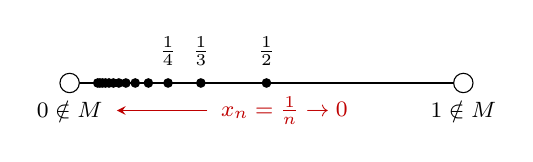
\begin{tikzpicture}[scale=5, >=stealth]
    \draw[thick] (0,0) -- (1,0);
    \foreach \n in {2,...,14} \fill ({1/\n},0) circle (0.35pt);
    \draw[fill=white] (0,0) circle (0.7pt);
    \draw[fill=white] (1,0) circle (0.7pt);
    \node[below] at (0,-0.02) {$0 \notin M$};
    \node[below] at (1,-0.02) {$1 \notin M$};
    \node[above] at (0.5,0.02) {$\tfrac12$};
    \node[above] at (0.3333,0.02) {$\tfrac13$};
    \node[above] at (0.25,0.02) {$\tfrac14$};
    \draw[->, red!75!black] (0.35,-0.07) -- (0.12,-0.07);
    \node[red!75!black, anchor=west] at (0.36,-0.07) {$x_n = \tfrac1n \to 0$};
\end{tikzpicture}
\end{center}
In $M = (0,1)$ the Cauchy sequence $x_n = 1/n$ ($n \ge 2$) heads for $0$, which is not in $M$; the completion supplies the missing point.
\end{exbox}

\subsection{Completion of a Normed Linear Space}

For a normed linear space $X$, the completion $\overline{X}$ as a metric space should again be a normed linear space, with $X$ sitting inside it as a subspace and with the original norm. The natural candidate for the norm of a class is the limit of the norms of a representative.

\begin{thmbox}[The Completion of a Normed Space is a Banach Space]\boxlabel{thm:completion-normed}
Let $(X, \|\cdot\|)$ be a normed linear space and $\overline{X}$ its completion. For a Cauchy sequence $\{x_n\}$ in $X$, write $[\{x_n\}] \in \overline{X}$ for its class, and define
\[
\bigl\| [\{x_n\}] \bigr\| := \lim_{n \to \infty} \|x_n\|.
\]
Then $\overline{X}$ is a linear space, this is a well-defined norm on it, $\|[(x, x, \ldots)]\| = \|x\|$ for $x \in X$, and $(\overline{X}, \|\cdot\|)$ is complete.
\laxref{\S5.1, Thm~3}
\end{thmbox}

\begin{notebox}[Notation for the Proof]\label{note:notation-proof}
The norm of $X$ is written $\|\cdot\|$ and the candidate norm on $\overline{X}$ is written $\|\cdot\|_{\overline{X}}$. A sequence in $\overline{X}$ is a sequence of classes; its $m$-th term is written $[\{x^{(m)}_n\}_n]$, where $\{x^{(m)}_n\}_n$ is a Cauchy sequence in $X$ (superscript: which class; subscript: which term of the representative).
\end{notebox}

\begin{proof}
(HW2, Problem 3.) Throughout, $\{x_n\}$ denotes a Cauchy sequence in $(X, \|\cdot\|)$ and $[\{x_n\}]$ its class in $\overline{X}$; two Cauchy sequences are equivalent iff $\lim_n \|x_n - y_n\| = 0$.

\textbf{Step 1: the limit $\lim_n \|x_n\|$ exists.} For all $m, k$, the reverse triangle inequality (Lemma~\ref{lem:reverse-triangle}) gives $\bigl|\,\|x_m\| - \|x_k\|\,\bigr| \le \|x_m - x_k\|$. Given $\varepsilon > 0$, choose $N$ with $\|x_m - x_k\| < \varepsilon$ for all $m, k > N$; then $\bigl|\,\|x_m\| - \|x_k\|\,\bigr| < \varepsilon$ for all $m, k > N$. So $\{\|x_n\|\}$ is a Cauchy sequence of real numbers, and since $\mathbb{R}$ is complete, $\lim_n \|x_n\|$ exists.

\textbf{Step 2: $\sim$ is an equivalence relation.} \emph{Reflexive:} $\lim_n \|x_n - x_n\| = \lim_n 0 = 0$. \emph{Symmetric:} since $\|y_n - x_n\| = \|x_n - y_n\|$ for every $n$, $\lim_n \|x_n - y_n\| = 0$ implies $\lim_n \|y_n - x_n\| = 0$. \emph{Transitive:} if $\lim_n \|x_n - y_n\| = 0$ and $\lim_n \|y_n - z_n\| = 0$, then by the triangle inequality
\[
0 \le \|x_n - z_n\| \le \|x_n - y_n\| + \|y_n - z_n\| \to 0 + 0 = 0,
\]
and limits preserve non-strict inequalities, so $\lim_n \|x_n - z_n\| = 0$.

\textbf{Step 3: $\|\cdot\|_{\overline{X}}$ is well defined.} Suppose $\{x_n\} \sim \{x_n'\}$. By the reverse triangle inequality, $0 \le \bigl|\,\|x_n\| - \|x_n'\|\,\bigr| \le \|x_n - x_n'\|$, so $\lim_n \bigl(\|x_n\| - \|x_n'\|\bigr) = 0$. Both limits exist by Step 1, so by linearity of limits $\lim_n \|x_n\| - \lim_n \|x_n'\| = 0$. Hence $\|[\{x_n\}]\|_{\overline{X}} = \lim_n \|x_n\|$ does not depend on the representative.

\textbf{Step 4: the operations on $\overline{X}$ are well defined.} Define $[\{x_n\}] + [\{y_n\}] = [\{x_n + y_n\}]$ and $a[\{x_n\}] = [\{a x_n\}]$.

\emph{The results are Cauchy sequences.} Given $\varepsilon > 0$, choose $N$ with $\|x_m - x_k\| < \varepsilon/2$ and $\|y_m - y_k\| < \varepsilon/2$ for $m, k > N$; then $\|(x_m + y_m) - (x_k + y_k)\| \le \|x_m - x_k\| + \|y_m - y_k\| < \varepsilon$. For $a \neq 0$, choose $N$ with $\|x_m - x_k\| < \varepsilon/|a|$ for $m, k > N$; then $\|a x_m - a x_k\| = |a|\,\|x_m - x_k\| < \varepsilon$. For $a = 0$ the sequence is constantly $0$, hence Cauchy.

\emph{Independence of representatives.} If $\{x_n\} \sim \{x_n'\}$ and $\{y_n\} \sim \{y_n'\}$, then
\[
\|(x_n + y_n) - (x_n' + y_n')\| \le \|x_n - x_n'\| + \|y_n - y_n'\| \to 0, \qquad \|a x_n - a x_n'\| = |a|\,\|x_n - x_n'\| \to 0,
\]
so $\{x_n + y_n\} \sim \{x_n' + y_n'\}$ and $\{a x_n\} \sim \{a x_n'\}$.

\textbf{Step 5: $\overline{X}$ is a linear space.} In each line the outer equalities use the definition of the operations on classes and the middle equality is the corresponding axiom of $X$, applied at each index $n$. Let $[\{x_n\}], [\{y_n\}], [\{z_n\}] \in \overline{X}$ and $a, k \in \mathbb{F}$.

\emph{Commutativity:} $[\{x_n\}] + [\{y_n\}] = [\{x_n + y_n\}] = [\{y_n + x_n\}] = [\{y_n\}] + [\{x_n\}]$.

\emph{Associativity:} $\bigl([\{x_n\}] + [\{y_n\}]\bigr) + [\{z_n\}] = [\{(x_n + y_n) + z_n\}] = [\{x_n + (y_n + z_n)\}] = [\{x_n\}] + \bigl([\{y_n\}] + [\{z_n\}]\bigr)$.

\emph{Additive identity:} the constant sequence $\{0\}$ is Cauchy, and $[\{x_n\}] + [\{0\}] = [\{x_n + 0\}] = [\{x_n\}] = [\{0 + x_n\}] = [\{0\}] + [\{x_n\}]$.

\emph{Additive inverse:} $\{-x_n\}$ is Cauchy (Step 4 with $a = -1$), and $[\{x_n\}] + [\{-x_n\}] = [\{x_n - x_n\}] = [\{0\}] = [\{-x_n + x_n\}] = [\{-x_n\}] + [\{x_n\}]$.

\emph{Compatibility:} $k\bigl(a[\{x_n\}]\bigr) = k[\{a x_n\}] = [\{k(a x_n)\}] = [\{(ka)x_n\}] = (ka)[\{x_n\}]$.

\emph{Distributivity over vector addition:} $k\bigl([\{x_n\}] + [\{y_n\}]\bigr) = [\{k(x_n + y_n)\}] = [\{k x_n + k y_n\}] = k[\{x_n\}] + k[\{y_n\}]$.

\emph{Distributivity over scalar addition:} $(a + k)[\{x_n\}] = [\{(a + k)x_n\}] = [\{a x_n + k x_n\}] = a[\{x_n\}] + k[\{x_n\}]$.

\emph{Unit:} $1[\{x_n\}] = [\{1 \cdot x_n\}] = [\{x_n\}]$.

Hence $\overline{X}$ is a linear space over $\mathbb{F}$ with zero element $[\{0\}]$.

\textbf{Step 6: $\|\cdot\|_{\overline{X}}$ is a norm.} \emph{Positivity.} Each $\|x_n\| \ge 0$, so $\lim_n \|x_n\| \ge 0$. If $\|[\{x_n\}]\|_{\overline{X}} = 0$, then $\lim_n \|x_n - 0\| = 0$, so $\{x_n\} \sim \{0\}$ and $[\{x_n\}] = [\{0\}]$. Conversely, if $[\{x_n\}] = [\{0\}]$ then $\lim_n \|x_n\| = 0$.

\emph{Homogeneity.} By Step 3 it suffices to compute with one representative: $\|a[\{x_n\}]\|_{\overline{X}} = \lim_n \|a x_n\| = \lim_n |a|\,\|x_n\| = |a| \lim_n \|x_n\| = |a|\,\|[\{x_n\}]\|_{\overline{X}}$.

\emph{Triangle inequality.} For every $n$, $\|x_n + y_n\| \le \|x_n\| + \|y_n\|$; all three limits exist by Step 1, and limits preserve non-strict inequalities, so
\[
\|[\{x_n\}] + [\{y_n\}]\|_{\overline{X}} = \lim_n \|x_n + y_n\| \le \lim_n \|x_n\| + \lim_n \|y_n\| = \|[\{x_n\}]\|_{\overline{X}} + \|[\{y_n\}]\|_{\overline{X}} .
\]
\emph{Extension.} For $x \in X$, $\|[(x, x, \ldots)]\|_{\overline{X}} = \lim_n \|x\| = \|x\|$.

\textbf{Step 7: construction of a candidate limit.} Let $\bigl([\{x^{(m)}_n\}_n]\bigr)_{m \ge 1}$ be Cauchy in $\overline{X}$. We build a sequence $\{y_j\}$ in $X$ by choosing, for each $j$, a sequence index $M_j$ and a term index $N_j$: one term out of one representative for each $j$, a diagonal choice.

\emph{Choice of the sequence indices.} Applying the Cauchy property with $\varepsilon = 1/j$, there is $m_j$ with $\|[\{x^{(m)}_n\}] - [\{x^{(k)}_n\}]\|_{\overline{X}} < 1/j$ for all $m, k \ge m_j$. Set $M_j = \max\{m_1, \ldots, m_j\}$, so that $M_1 \le M_2 \le \cdots$ and $M_j \ge m_j$. The condition then holds for all indices $\ge M_j$; taking $k = M_j$,
\begin{equation}\label{eq:comp1}
\bigl\| [\{x^{(M_j)}_n\}] - [\{x^{(m)}_n\}] \bigr\|_{\overline{X}} = \lim_{n \to \infty} \bigl\| x^{(M_j)}_n - x^{(m)}_n \bigr\| < \frac{1}{j} \qquad \text{for all } m \ge M_j.
\end{equation}

\emph{Choice of the term indices.} With the $M_j$ fixed, each $\{x^{(M_j)}_n\}_n$ is Cauchy in $X$, so there is $n_j$ with $\|x^{(M_j)}_n - x^{(M_j)}_{n'}\| < 1/j$ for all $n, n' \ge n_j$. Set $N_j = \max\{n_1, \ldots, n_j\}$, so $N_1 \le N_2 \le \cdots$ and
\begin{equation}\label{eq:comp2}
\bigl\| x^{(M_j)}_n - x^{(M_j)}_{n'} \bigr\| < \frac{1}{j} \qquad \text{for all } n, n' \ge N_j.
\end{equation}

\emph{The candidate.} Define $y_j := x^{(M_j)}_{N_j} \in X$, the $N_j$-th term of the $M_j$-th sequence. Property \eqref{eq:comp1} compares the sequence $\{x^{(M_j)}_n\}_n$ to every later sequence in the norm of $\overline{X}$; property \eqref{eq:comp2} compares terms of that one sequence to each other.

\textbf{Step 8: $\{y_j\}$ is Cauchy in $X$.} Let $\varepsilon > 0$ and choose $J$ with $3/J < \varepsilon$. Take $j, k \ge J$; since $\|y_j - y_k\| = \|y_k - y_j\|$ and the case $j = k$ is trivial, assume $j > k \ge J$. For any index $n'$, inserting two intermediate terms,
\[
\|y_j - y_k\| \le \underbrace{\bigl\| x^{(M_j)}_{N_j} - x^{(M_j)}_{n'} \bigr\|}_{\textcircled{1}} + \underbrace{\bigl\| x^{(M_j)}_{n'} - x^{(M_k)}_{n'} \bigr\|}_{\textcircled{2}} + \underbrace{\bigl\| x^{(M_k)}_{n'} - x^{(M_k)}_{N_k} \bigr\|}_{\textcircled{3}} .
\]
\emph{Term \textcircled{1}.} Both term indices belong to the single sequence $\{x^{(M_j)}_n\}_n$; by \eqref{eq:comp2} at index $j$, if $n' \ge N_j$ then $\textcircled{1} < 1/j$.

\emph{Term \textcircled{3}.} Likewise, by \eqref{eq:comp2} at index $k$, if $n' \ge N_k$ then $\textcircled{3} < 1/k$.

\emph{Term \textcircled{2}.} The two entries come from different sequences at the same term index. Since $j > k$ and $\{M_j\}$ is non-decreasing, $M_j \ge M_k$, so \eqref{eq:comp1} at index $k$ applies with $m = M_j$: $\lim_{n} \|x^{(M_k)}_n - x^{(M_j)}_n\| < 1/k$. A sequence of reals whose limit is $< 1/k$ is eventually $< 1/k$, so there is $N$ (depending on $j$ and $k$) with $\textcircled{2} < 1/k$ for all $n' \ge N$.

\emph{Choice of $n'$.} Take $n' \ge \max\{N_j, N_k, N\}$. All three bounds hold, and since $1/j < 1/k \le 1/J$,
\[
\|y_j - y_k\| < \frac{1}{j} + \frac{1}{k} + \frac{1}{k} \le \frac{3}{J} < \varepsilon .
\]
Here $n'$ was chosen after $j$ and $k$ were fixed and does not appear in the conclusion. Hence $\{y_j\}$ is Cauchy in $X$, and $[\{y_j\}] \in \overline{X}$.

\textbf{Step 9: $[\{x^{(m)}_n\}] \to [\{y_n\}]$ in $\overline{X}$.} Let $\varepsilon > 0$ and fix $j$ with $3/j < \varepsilon$. For any $m \ge M_j$,
\begin{equation}\label{eq:comp3}
\bigl\| [\{x^{(m)}_n\}] - [\{y_n\}] \bigr\|_{\overline{X}} \le \underbrace{\bigl\| [\{x^{(m)}_n\}] - [\{x^{(M_j)}_n\}] \bigr\|_{\overline{X}}}_{\textcircled{A}} + \underbrace{\bigl\| [\{x^{(M_j)}_n\}] - [\{y_n\}] \bigr\|_{\overline{X}}}_{\textcircled{B}} .
\end{equation}
\emph{Term \textcircled{A}.} Since $m \ge M_j$, \eqref{eq:comp1} at index $j$ gives $\textcircled{A} < 1/j$.

\emph{Term \textcircled{B}.} We claim $\textcircled{B} \le 2/j$. By definition, $\textcircled{B} = \lim_n \|x^{(M_j)}_n - y_n\| = \lim_n \|x^{(M_j)}_n - x^{(M_n)}_{N_n}\|$, so it suffices to bound $\|x^{(M_j)}_n - x^{(M_n)}_{N_n}\|$ for all large $n$. Let $n \ge \max\{j, N_j\}$. For any auxiliary index $n'$,
\[
\bigl\| x^{(M_j)}_n - x^{(M_n)}_{N_n} \bigr\| \le \underbrace{\bigl\| x^{(M_j)}_n - x^{(M_j)}_{n'} \bigr\|}_{\textcircled{1}} + \underbrace{\bigl\| x^{(M_j)}_{n'} - x^{(M_n)}_{n'} \bigr\|}_{\textcircled{2}} + \underbrace{\bigl\| x^{(M_n)}_{n'} - x^{(M_n)}_{N_n} \bigr\|}_{\textcircled{3}} .
\]
For \textcircled{1}: both term indices lie in $\{x^{(M_j)}_n\}_n$, so by \eqref{eq:comp2} at index $j$, if $n' \ge N_j$ (and $n \ge N_j$, which holds) then $\textcircled{1} < 1/j$. For \textcircled{2}: since $n \ge j$ and $\{M_n\}$ is non-decreasing, $M_n \ge M_j$, so \eqref{eq:comp1} at index $j$ with $m = M_n$ gives $\lim_{n'} \|x^{(M_j)}_{n'} - x^{(M_n)}_{n'}\| < 1/j$, and there is $P$ (depending on $j$ and $n$) with $\textcircled{2} < 1/j$ for all $n' \ge P$. For \textcircled{3}: both term indices lie in $\{x^{(M_n)}_{n'}\}_{n'}$, so by \eqref{eq:comp2} at index $n$, if $n' \ge N_n$ then $\textcircled{3} < 1/n$. Taking $n' \ge \max\{N_j, N_n, P\}$, all three bounds hold and $n'$ disappears:
\[
\bigl\| x^{(M_j)}_n - x^{(M_n)}_{N_n} \bigr\| < \frac{2}{j} + \frac{1}{n} \qquad \text{for all } n \ge \max\{j, N_j\}.
\]
Letting $n \to \infty$, $\textcircled{B} \le 2/j$.

\emph{Conclusion.} By \eqref{eq:comp3}, for every $m \ge M_j$, $\|[\{x^{(m)}_n\}] - [\{y_n\}]\|_{\overline{X}} < 1/j + 2/j = 3/j < \varepsilon$. So the Cauchy sequence converges in $\overline{X}$ to $[\{y_n\}]$, and $(\overline{X}, \|\cdot\|_{\overline{X}})$ is complete; with Steps 5 and 6 it is a Banach space.
\end{proof}

\begin{rembox}[Comparison with the $\ell^p$ Proof]\label{rem:comparison-l-p-proof}
The structure is the one from Theorem~\ref{thm:lp-complete}, with the roles shifted. In $\ell^p$ the candidate came from coordinates and the closing step needed a uniform tail estimate obtained by truncating. Here the candidate is a \emph{diagonal} sequence $y_j = x^{(M_j)}_{N_j}$: one term from each representative, chosen far enough out that within-representative fluctuations \eqref{eq:comp2} and between-representative distances \eqref{eq:comp1} are both below $1/j$. The closing step is the same three-term triangle inequality used twice, with an auxiliary index $n'$ that is sent far out after everything else is fixed and then disappears. The two monotone index sequences $M_j, N_j$ are what make ``$m = M_n \ge M_j$ when $n \ge j$'' available; without the $\max$ in their definition the comparisons in \eqref{eq:comp1} could not be applied in the direction needed.
\end{rembox}

\begin{rembox}\label{rem:completeness-3}
A student asked whether one could define the norm of a class as the norm of its limit. There is no limit in $X$ to speak of --- that is the whole reason for the construction --- so the definition must be phrased in terms of the sequence itself, and existence of $\lim \|x_n\|$ is then a claim to prove, not a definition. The relevant estimate is the reverse triangle inequality (Lemma~\ref{lem:reverse-triangle}), $\bigl|\,\|x_m\| - \|x_k\|\,\bigr| \le \|x_m - x_k\|$, which makes $\{\|x_n\|\}$ a Cauchy sequence of real numbers.
\end{rembox}

% Lecture 6 (2026-09-17)
\subsection{Identifying a Completion}

The construction by equivalence classes is abstract, but in practice the completion of a concrete space can almost always be written down as a concrete space. The following proposition is the tool: if the space is already sitting densely inside something complete, that something \emph{is} the completion.

\begin{propbox}[Identifying a Completion]\boxlabel{prop:identify-completion}
Let $(X, \|\cdot\|_X)$ be a normed linear space, $(Z, \|\cdot\|_Z)$ a Banach space, and $J : X \to Z$ a linear map with $\|Jx\|_Z = \|x\|_X$ for all $x \in X$, such that $J(X)$ is dense in $Z$. Then
\[
\Phi : \overline{X} \to Z, \qquad \Phi\bigl([\{x_n\}]\bigr) = \lim_{n \to \infty} J x_n,
\]
is an isometric isomorphism of $\overline{X}$ onto $Z$, and it sends the class of the constant sequence $(x, x, \ldots)$ to $Jx$. In particular, if $X \subset Z$ is a dense linear subspace carrying the restricted norm ($J$ the inclusion), then $\overline{X}$ is isometrically isomorphic to $Z$ by an isomorphism that is the identity on $X$.
\end{propbox}

\begin{proof}
(Not covered in lecture.) \emph{The limit exists.} If $\{x_n\}$ is Cauchy in $X$, then $\|Jx_n - Jx_m\|_Z = \|J(x_n - x_m)\|_Z = \|x_n - x_m\|_X$, so $\{Jx_n\}$ is Cauchy in $Z$, and it converges because $Z$ is complete.

\emph{Well defined.} If $\{x_n\} \sim \{x_n'\}$ then $\|Jx_n - Jx_n'\|_Z = \|x_n - x_n'\|_X \to 0$, so the two limits coincide.

\emph{Linear.} The operations on $\overline{X}$ are termwise, $J$ is linear, and limits in $Z$ are linear.

\emph{Isometric.} By continuity of the norm (Proposition~\ref{prop:norm-continuous}),
\[
\|\Phi([\{x_n\}])\|_Z = \lim_n \|Jx_n\|_Z = \lim_n \|x_n\|_X = \|[\{x_n\}]\|,
\]
the last equality being the definition of the norm on $\overline{X}$. An isometry is injective: $\Phi(\xi) = 0$ forces $\|\xi\| = 0$, hence $\xi = 0$.

\emph{Surjective.} Let $z \in Z$. By density there are $x_n \in X$ with $Jx_n \to z$. A convergent sequence is Cauchy (Proposition~\ref{prop:conv-basic}), and $\|x_n - x_m\|_X = \|Jx_n - Jx_m\|_Z$, so $\{x_n\}$ is Cauchy in $X$ and $\Phi([\{x_n\}]) = z$.

Finally $\Phi([(x, x, \ldots)]) = \lim_n Jx = Jx$.
\end{proof}

\begin{rembox}\label{rem:completeness-4}
The embedding form is needed in practice: an element of $L^p[a,b]$ is a class of functions equal almost everywhere, so $C[a,b]$ is not literally a subset of $L^p[a,b]$; it sits inside via $f \mapsto [f]$. The proposition is the precise meaning of ``$Z$ \emph{is} the completion of $X$'': the abstract $\overline{X}$ and the concrete $Z$ are the same Banach space, with $X$ corresponding to $J(X)$.
\end{rembox}

\begin{corbox}[Uniqueness of the Completion]\boxlabel{cor:completion-unique}
Let $X$ be a normed linear space. If $Z_1$ and $Z_2$ are Banach spaces each containing $X$ as a dense subspace with the same norm, then $Z_1$ and $Z_2$ are isometrically isomorphic by a map fixing $X$. In this sense the completion of $X$ is unique.
\end{corbox}

\begin{proof}
(Stated in lecture without proof; the proof is not from lecture.) Both are isometrically isomorphic to $\overline{X}$ by Proposition~\ref{prop:identify-completion}; compose one isomorphism with the inverse of the other (Lemma~\ref{lem:inverse-iso}).
\end{proof}

\begin{rembox}[{{``How Do We Know We Have Not Added Too Much?''}}]\label{rem:how-do-we-know-we-have-not-added-too-much}
This was asked in lecture, and Corollary~\ref{cor:completion-unique} is the answer: there is no freedom. The construction adds only limits of Cauchy sequences in $X$ and identifies two sequences whenever they head for the same place, so nothing extra can appear.

A larger complete space containing $X$ need not be the completion. A student's example: with the usual absolute value, the completion of $\mathbb{Q}$ is $\mathbb{R}$, and $\mathbb{R} \subset \mathbb{C}$ with $\mathbb{C}$ complete --- but $\mathbb{C}$ is not the completion of $\mathbb{Q}$, because a Cauchy sequence of rationals cannot converge to a non-real number. Equivalently in Wu's version, $\mathbb{R} \subset \mathbb{R}^2$ is a complete space containing $\mathbb{R}$, and is not its completion. The condition that fails is density.

Also worth separating: the definition of $\overline{X}$ is by equivalence classes, and the description ``$X$ together with all its limit points'' is a way of thinking, not a definition --- before the construction there is no ambient space in which those limit points live. Wu: ``the previous one is more precise; the later one is a way of thinking. What is the limit when you don't even have a point?''
\end{rembox}

\begin{rembox}[{{The Norm Decides, Not the Set}}]\label{rem:norm-decides-not-set}
A second trap. As \emph{sets}, $C[a,b] \subset L^1[a,b]$, and $L^1[a,b]$ is complete; but $L^1[a,b]$ is not the completion of $\bigl(C[a,b], \|\cdot\|_\infty\bigr)$, which is already complete (Theorem~\ref{thm:Cab-banach}) and is therefore its own completion. The two norms $\|\cdot\|_\infty$ and $\|\cdot\|_{L^1}$ are not equivalent, so they give different topologies, different Cauchy sequences, and different completions. A normed linear space is the pair $(X, \|\cdot\|)$, never the set alone; the completion is determined by the norm. The same set $C[a,b]$ with the $L^p$ norm, $1 \le p < \infty$, does have completion $L^p[a,b]$ (\S\ref{subsec:completion-L1}).
\end{rembox}

\subsection{An Incomplete Normed Space}

\begin{exbox}[{{$C^2[a,b]$ with a $C^1$ Norm}}]\boxlabel{ex:c2-a-b-c1-norm}
Let $C^k[a,b]$ denote the $k$ times continuously differentiable functions on $[a,b]$. The natural norm on $C^2[a,b]$ is
\[
\|f\|_{C^2[a,b]} = \max_{[a,b]} |f| + \max_{[a,b]} |f'| + \max_{[a,b]} |f''|,
\]
and $(C^2[a,b], \|\cdot\|_{C^2})$ is complete, by the same argument as for $C[a,b]$ (Theorem~\ref{thm:Cab-banach}) applied to $f$, $f'$, $f''$ simultaneously. But the set $X = C^2[a,b]$ may also be given the smaller norm
\[
\|f\|_X = \max_{[a,b]} |f| + \max_{[a,b]} |f'|,
\]
which omits the second derivative, and $(X, \|\cdot\|_X)$ is a normed linear space that is \emph{not} complete. This is another instance of the previous remark: the same set, two inequivalent norms, one complete and one not.
\end{exbox}

\begin{propbox}[{{$(C^2[a,b], \|\cdot\|_X)$ is Not Complete}}]\boxlabel{prop:C2-incomplete}
With $\|f\|_X = \max |f| + \max |f'|$, the space $X = C^2[a,b]$ is not complete, and its completion is $C^1[a,b]$ with the same norm.
\end{propbox}

\begin{proof}
(HW3, Problem 2.) 
Throughout, $C^k([a,b])$ ($k = 1, 2$) denotes the functions $f : [a,b] \to \mathbb{F}$ that are $k$ times differentiable on $[a,b]$ (one-sided at the endpoints) with $f^{(k)}$ continuous, and $\|g\|_\infty = \max_{[a,b]} |g|$ for $g \in C([a,b])$; $(C([a,b]), \|\cdot\|_\infty)$ is a Banach space (Theorem~\ref{thm:Cab-banach}). Write $\|f\| = \|f\|_X = \|f\|_\infty + \|f'\|_\infty$. For complex-valued functions, differentiation and integration act on real and imaginary parts, so the fundamental theorem of calculus holds, and $\bigl|\int_\alpha^\beta h\bigr| \leq \int_\alpha^\beta |h|$ for continuous $h$. We show that $(X, \|\cdot\|)$ is a normed linear space, that it is \emph{not} complete, and that its completion is $C^1([a,b])$ with the same norm.

\textbf{Part 1: $(X, \|\cdot\|)$ is a normed linear space.} If $f, g \in X$ and $c \in \mathbb{F}$, then $(f + g)' = f' + g'$, $(f+g)'' = f'' + g''$, $(cf)' = cf'$ and $(cf)'' = cf''$, all continuous; so $X$ is a linear subspace of $C([a,b])$, hence a linear space. The norm is well defined because $f$ and $f'$ are continuous on $[a,b]$, so both maxima exist.

\emph{Positivity.} $\|f\| \geq 0$. If $\|f\| = 0$, then $\|f\|_\infty = 0$, since both terms are non-negative; so $f = 0$.

\emph{Homogeneity.} $\|cf\| = \|cf\|_\infty + \|cf'\|_\infty = |c|\,\|f\|_\infty + |c|\,\|f'\|_\infty = |c|\,\|f\|$.

\emph{Triangle inequality.} By the triangle inequality for $\|\cdot\|_\infty$,
\[\|f + g\| = \|f + g\|_\infty + \|f' + g'\|_\infty \leq \|f\|_\infty + \|g\|_\infty + \|f'\|_\infty + \|g'\|_\infty = \|f\| + \|g\|.\]
The same computations, which use only the first derivative, show that $\|\cdot\|$ is also a norm on $C^1([a,b])$. Write $Z = (C^1([a,b]), \|\cdot\|)$; then $X \subset Z$, with the same norm.

\textbf{Part 2: $Z$ is complete.} Let $\{f_n\}$ be Cauchy in $Z$. Since $\|f_n - f_m\|_\infty \leq \|f_n - f_m\|$ and $\|f_n' - f_m'\|_\infty \leq \|f_n - f_m\|$, both $\{f_n\}$ and $\{f_n'\}$ are Cauchy in $(C([a,b]), \|\cdot\|_\infty)$, which is complete. So there are $f, g \in C([a,b])$ with
\[\|f_n - f\|_\infty \to 0, \qquad \|f_n' - g\|_\infty \to 0.\]
By the fundamental theorem of calculus, for every $n$ and every $x \in [a,b]$,
\[f_n(x) = f_n(a) + \int_a^x f_n'(t)\,dt.\]
Fix $x$. As $n \to \infty$, $f_n(x) \to f(x)$, $f_n(a) \to f(a)$, and
\[\Bigl| \int_a^x f_n'(t)\,dt - \int_a^x g(t)\,dt \Bigr| \leq \int_a^x |f_n' - g| \leq (b - a)\,\|f_n' - g\|_\infty \to 0.\]
Hence
\[f(x) = f(a) + \int_a^x g(t)\,dt \qquad \text{for all } x \in [a,b].\]
Since $g$ is continuous, the fundamental theorem of calculus shows that $f$ is differentiable on $[a,b]$ with $f' = g$. So $f \in C^1([a,b])$, and
\[\|f_n - f\| = \|f_n - f\|_\infty + \|f_n' - g\|_\infty \to 0.\]
Thus $Z$ is complete.

\textbf{Part 3: $X$ is dense in $Z$.} Let $f \in C^1([a,b])$ and $\varepsilon > 0$. Since $f'$ is continuous on $[a,b]$, the Weierstrass approximation theorem (applied to the real and imaginary parts if $\mathbb{F} = \mathbb{C}$) gives a polynomial $P$ with
\[\|P - f'\|_\infty < \frac{\varepsilon}{1 + b - a}.\]
Define
\[q(x) = f(a) + \int_a^x P(t)\,dt, \qquad x \in [a,b].\]
Then $q$ is a polynomial, so $q \in C^2([a,b]) = X$, and $q' = P$. Using $f(x) = f(a) + \int_a^x f'(t)\,dt$,
\[|q(x) - f(x)| = \Bigl| \int_a^x \bigl( P(t) - f'(t) \bigr)\,dt \Bigr| \leq (b - a)\,\|P - f'\|_\infty \qquad \text{for all } x \in [a,b].\]
Hence
\[\|q - f\| = \|q - f\|_\infty + \|P - f'\|_\infty \leq (1 + b - a)\,\|P - f'\|_\infty < \varepsilon.\]

\textbf{Part 4: $X \neq Z$.} Let $c = (a+b)/2$ and $\varphi(x) = |x - c|^{3/2}$. For $x \neq c$, the chain rule gives $\varphi'(x) = \frac32 \operatorname{sgn}(x - c)\,|x - c|^{1/2}$. At $x = c$,
\[\Bigl| \frac{\varphi(c + h) - \varphi(c)}{h} \Bigr| = |h|^{1/2} \xrightarrow[h \to 0]{} 0,\]
so $\varphi'(c) = 0$. Thus $\varphi'(x) = \frac32 \operatorname{sgn}(x - c)\,|x - c|^{1/2}$ for all $x$ (with $\operatorname{sgn} 0 = 0$), and $\varphi'$ is continuous on $[a,b]$: it is continuous away from $c$, and $|\varphi'(x)| = \frac32 |x - c|^{1/2} \to 0 = \varphi'(c)$ as $x \to c$. So $\varphi \in C^1([a,b])$. However,
\[\frac{\varphi'(c + h) - \varphi'(c)}{h} = \frac32 \cdot \frac{\operatorname{sgn}(h)\,|h|^{1/2}}{h} = \frac32\,|h|^{-1/2} \xrightarrow[h \to 0]{} \infty,\]
so $\varphi'$ is not differentiable at $c$, and $\varphi \notin C^2([a,b])$.

\textbf{Part 5: conclusion.}

\emph{$X$ is not complete.} By Part 3 there are $q_n \in X$ with $\|q_n - \varphi\| \to 0$. The sequence $\{q_n\}$ is Cauchy in $X$, since $\|q_n - q_m\| \leq \|q_n - \varphi\| + \|\varphi - q_m\|$. If it converged in $X$ to some $h \in X$, then, as $X$ carries the norm of $Z$, it would converge in $Z$ to both $h$ and $\varphi$. Limits in a metric space are unique, so $\varphi = h \in X$, contradicting Part 4. Hence $(X, \|\cdot\|)$ is not complete.

\emph{The completion.} The inclusion $J : X \to Z$ is linear and norm-preserving, $J(X) = X$ is dense in $Z$ by Part 3, and $Z$ is a Banach space by Part 2. By Proposition~\ref{prop:identify-completion}, the completion of $(X, \|\cdot\|)$ is
\[\Bigl( C^1([a,b]),\ \|f\| = \max_{t \in [a,b]} |f(t)| + \max_{t \in [a,b]} |f'(t)| \Bigr).\]
\end{proof}


% ============================================================================
% SECTION 10: NEW NORMED SPACES FROM OLD
% ============================================================================

\section{New Normed Spaces from Old}\label{sec:new-from-old}

\roadmark{Stage: norms}{Thread: dimension. In finite dimensions all norms are equivalent (Theorem~\ref{prop:norms-equiv}); subspaces, direct sums and quotients acquire norms.}

The constructions of Chapter 1 --- subspaces, direct sums, quotients --- each acquire a natural norm. The first two are immediate; the quotient requires a hypothesis and a proof.

\subsection{Equivalent Norms}\label{subsec:equiv-norms}

\begin{defbox}[Equivalent Norms]\boxlabel{def:equivalent-norms}
Let $X$ be a linear space with two norms $\|\cdot\|_1$ and $\|\cdot\|_2$. They are \textbf{equivalent} if there are constants $c_1, c_2 > 0$ such that
\[
c_1 \|x\|_2 \;\le\; \|x\|_1 \;\le\; c_2 \|x\|_2 \qquad \text{for all } x \in X.
\]
\laxref{\S5.1, (5)}
\end{defbox}

If $B_1$ and $B_2$ denote the closed unit balls of $\|\cdot\|_1$ and $\|\cdot\|_2$, the definition says exactly that $\tfrac{1}{c_2} B_2 \subset B_1 \subset \tfrac{1}{c_1} B_2$: if $\|x\|_1 \le 1$ then $\|x\|_2 \le 1/c_1$, and if $\|x\|_2 \le 1/c_2$ then $\|x\|_1 \le 1$. Each unit ball is squeezed between two scaled copies of the other.

\begin{center}
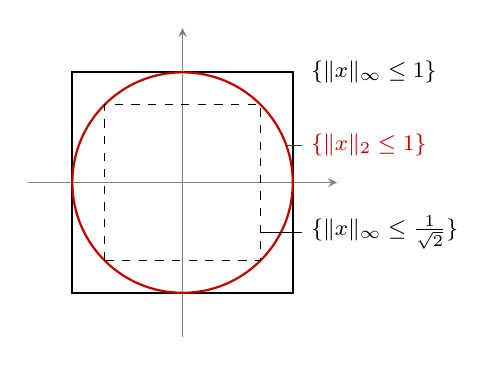
\begin{tikzpicture}[scale=1.4, >=stealth]
    \draw[->, gray] (-1.4,0) -- (1.4,0);
    \draw[->, gray] (0,-1.4) -- (0,1.4);
    \draw[thick] (-1,-1) rectangle (1,1);
    \draw[thick, red!75!black] (0,0) circle (1);
    \draw[dashed] (-0.7071,-0.7071) rectangle (0.7071,0.7071);
    \node[anchor=west] at (1.08,1) {$\{\|x\|_\infty \le 1\}$};
    \draw[thin, red!75!black] (0.94,0.34) -- (1.08,0.34);
    \node[anchor=west, red!75!black] at (1.08,0.34) {$\{\|x\|_2 \le 1\}$};
    \draw[thin] (0.7071,-0.45) -- (1.08,-0.45);
    \node[anchor=west] at (1.08,-0.45) {$\{\|x\|_\infty \le \tfrac{1}{\sqrt{2}}\}$};
\end{tikzpicture}
\end{center}
For the maximum and Euclidean norms on $\mathbb{R}^2$ (Example~\ref{ex:norms-rn}), $\|x\|_\infty \le \|x\|_2 \le \sqrt{2}\,\|x\|_\infty$: the disk contains the dashed square and lies inside the solid one.

The constants must work for all $x$ at once: the condition says that the ratio $\|x\|_1 / \|x\|_2$ is bounded above and below on $X \setminus \{0\}$. Its meaning is topological.

\begin{propbox}[Equivalent Norms Have the Same Convergence]\boxlabel{prop:equiv-same}
Let $\|\cdot\|_1$ and $\|\cdot\|_2$ be equivalent norms on $X$. Then a sequence converges to $x$ in $\|\cdot\|_1$ iff it converges to $x$ in $\|\cdot\|_2$; a sequence is Cauchy for $\|\cdot\|_1$ iff it is Cauchy for $\|\cdot\|_2$; a subset of $X$ is closed for $\|\cdot\|_1$ iff it is closed for $\|\cdot\|_2$; and $(X, \|\cdot\|_1)$ is complete iff $(X, \|\cdot\|_2)$ is.
\end{propbox}

\begin{proof}
(Not covered in lecture.) With $c_1\|x\|_2 \le \|x\|_1 \le c_2\|x\|_2$, we have $\|x_n - x\|_1 \le c_2\|x_n - x\|_2$ and $\|x_n - x\|_2 \le c_1^{-1}\|x_n - x\|_1$, so the two notions of convergence coincide; the same inequalities applied to $x_m - x_k$ give the statement about Cauchy sequences. Closedness (Definition~\ref{def:closed}) and completeness are defined through convergent and Cauchy sequences alone, so they coincide as well.
\end{proof}

\begin{propbox}[Continuity of One Norm with Respect to Another]\boxlabel{prop:norm-cont-other}
Let $\|\cdot\|_1$ and $\|\cdot\|_2$ be norms on $X$. Then $\|x_n - x\|_2 \to 0$ implies $\|x_n\|_1 \to \|x\|_1$ for all sequences if and only if there is a constant $C$ with $\|x\|_1 \le C\|x\|_2$ for all $x \in X$. Consequently the two norms are equivalent iff each is continuous with respect to the other in this sense.
\end{propbox}

\begin{proof}
($\Leftarrow$) By the reverse triangle inequality, $\bigl|\,\|x_n\|_1 - \|x\|_1\,\bigr| \le \|x_n - x\|_1 \le C\|x_n - x\|_2 \to 0$.

($\Rightarrow$) Suppose no such $C$ exists. Then for each $n$ there is $x_n$ with $\|x_n\|_1 > n\|x_n\|_2$; necessarily $x_n \neq 0$, so $\|x_n\|_2 > 0$. Put $z_n = x_n / (n\|x_n\|_2)$. Then $\|z_n\|_2 = 1/n \to 0$, so $z_n \to 0$ in $\|\cdot\|_2$, while $\|z_n\|_1 = \|x_n\|_1 / (n\|x_n\|_2) > 1$, so $\|z_n\|_1 \not\to 0 = \|0\|_1$. This contradicts the continuity. (Not covered in lecture.)
\end{proof}

\begin{rembox}\label{rem:new-from-old}
Anything defined in terms of convergence cannot tell equivalent norms apart. Conversely, two norms on one set for which the space is complete under one and not under the other cannot be equivalent --- as for $\|\cdot\|_\infty$ and $\|\cdot\|_{L^1}$ on $C[a,b]$.
\end{rembox}

\begin{thmbox}[All Norms on a Finite-Dimensional Space are Equivalent]\boxlabel{prop:norms-equiv}
Let $X$ be a finite-dimensional linear space over $\mathbb{F}$. Any two norms on $X$ are equivalent.
\end{thmbox}

\begin{proof}
(HW2, Problem 2(a).) Since $X$ is finite dimensional, it has a basis $\{e_1, \ldots, e_n\}$, and every $x \in X$ can be written uniquely as $x = \sum_{i=1}^n a_i e_i$ with $a_i \in \mathbb{F}$. Two norms $\|\cdot\|_a$ and $\|\cdot\|_b$ on $X$ are equivalent, written $\|\cdot\|_a \sim \|\cdot\|_b$, if there are constants $c, C > 0$ with $c\,\|x\|_a \le \|x\|_b \le C\,\|x\|_a$ for all $x$.

\textbf{Step 1: equivalence of norms is an equivalence relation.} \emph{Reflexivity:} $1 \cdot \|x\|_a \le \|x\|_a \le 1 \cdot \|x\|_a$. \emph{Symmetry:} suppose $c_1\|x\|_a \le \|x\|_b \le c_2\|x\|_a$ for all $x$, with $c_1, c_2 > 0$. Dividing the right-hand inequality by $c_2$ gives $\frac{1}{c_2}\|x\|_b \le \|x\|_a$, and dividing the left-hand one by $c_1$ gives $\|x\|_a \le \frac{1}{c_1}\|x\|_b$; hence $\frac{1}{c_2}\|x\|_b \le \|x\|_a \le \frac{1}{c_1}\|x\|_b$. \emph{Transitivity:} if $c_1\|x\|_a \le \|x\|_b \le c_2\|x\|_a$ and $d_1\|x\|_b \le \|x\|_c \le d_2\|x\|_b$ for all $x$, with all four constants positive, then
\[
d_1 c_1\,\|x\|_a \le d_1\,\|x\|_b \le \|x\|_c \le d_2\,\|x\|_b \le d_2 c_2\,\|x\|_a .
\]

\textbf{Step 2: a reference norm.} Define $\|x\|_1 = \sum_{i=1}^n |a_i|$ for $x = \sum_i a_i e_i$. \emph{Positivity:} each $|a_i| \ge 0$, so $\|x\|_1 \ge 0$; if $\|x\|_1 = 0$ then every $a_i = 0$ and $x = 0$; conversely if $x = 0$ then all $a_i = 0$ by uniqueness of the expansion, and $\|x\|_1 = 0$. \emph{Homogeneity:} $kx = \sum_i (k a_i) e_i$, so $\|kx\|_1 = \sum_i |k a_i| = |k|\,\|x\|_1$. \emph{Triangle inequality:} for $x = \sum a_i e_i$, $y = \sum b_i e_i$, $x + y = \sum (a_i + b_i) e_i$ and $\|x + y\|_1 = \sum_i |a_i + b_i| \le \sum_i (|a_i| + |b_i|) = \|x\|_1 + \|y\|_1$. By Step 1 it suffices to prove that an arbitrary norm $\|\cdot\|'$ on $X$ is equivalent to $\|\cdot\|_1$.

\textbf{Step 3: the inequality $C_1\|x\|' \le \|x\|_1$.} Fix a norm $\|\cdot\|'$. For each $i$, both $\|e_i\|'$ and $\|e_i\|_1 = 1$ are positive reals, so there is $c_i > 0$ with $c_i\|e_i\|' = \|e_i\|_1 = 1$. The finite set $\{c_1, \ldots, c_n\}$ has a minimum $C_1 = \min_i c_i > 0$, and for every $i$,
\[
C_1 \|e_i\|' \le c_i \|e_i\|' = 1 = \|e_i\|_1 .
\]
Multiplying by $|a_i| \ge 0$ and using homogeneity, $C_1\|a_i e_i\|' = C_1|a_i|\,\|e_i\|' \le |a_i|\,\|e_i\|_1 = |a_i|$. For $x = \sum_i a_i e_i$, subadditivity of $\|\cdot\|'$ and the above, summed over $i$, give
\[
C_1\|x\|' \le C_1 \sum_{i=1}^n \|a_i e_i\|' \le \sum_{i=1}^n |a_i| = \|x\|_1 .
\]

\textbf{Step 4: $\|\cdot\|'$ is continuous on $(X, \|\cdot\|_1)$.} By Step 3, $\|z\|' \le \frac{1}{C_1}\|z\|_1$ for every $z$. Hence, by the reverse triangle inequality for $\|\cdot\|'$,
\[
\bigl|\,\|x\|' - \|y\|'\,\bigr| \le \|x - y\|' \le \frac{1}{C_1}\,\|x - y\|_1 .
\]
Given $\varepsilon > 0$, take $\delta = C_1\varepsilon$: if $\|x - y\|_1 < \delta$ then $\bigl|\,\|x\|' - \|y\|'\,\bigr| < \varepsilon$. So $\|\cdot\|' : X \to \mathbb{R}$ is continuous when distances in $X$ are measured by $\|\cdot\|_1$.

\textbf{Step 5: the unit sphere of $\|\cdot\|_1$ is sequentially compact.} Let $S = \{x \in X : \|x\|_1 = 1\}$ and let $\{x^{(k)}\} \subset S$, $x^{(k)} = \sum_i a^{(k)}_i e_i$. Each coordinate sequence is bounded, $|a^{(k)}_i| \le \|x^{(k)}\|_1 = 1$. By Bolzano--Weierstrass in $\mathbb{F}$ applied $n$ times --- extract a subsequence along which $a^{(k)}_1$ converges, then a further subsequence along which $a^{(k)}_2$ converges, and so on --- there is a subsequence $\{x^{(k_r)}\}$ with $a^{(k_r)}_i \to a_i$ for every $i = 1, \ldots, n$. Put $x = \sum_i a_i e_i$. Then $\|x^{(k_r)} - x\|_1 = \sum_i |a^{(k_r)}_i - a_i| \to 0$ (a finite sum of terms tending to $0$), and $\|x\|_1 = \sum_i |a_i| = \lim_r \sum_i |a^{(k_r)}_i| = 1$, so $x \in S$. Thus every sequence in $S$ has a subsequence converging in $\|\cdot\|_1$ to a point of $S$.

\textbf{Step 6: $\|\cdot\|'$ attains a positive minimum on $S$.} Let $c = \inf_{x \in S} \|x\|' \ge 0$. Choose $x^{(k)} \in S$ with $\|x^{(k)}\|' \to c$, and by Step 5 a subsequence $x^{(k_r)} \to x^* \in S$ in $\|\cdot\|_1$. By Step 4, $\|x^{(k_r)}\|' \to \|x^*\|'$, so $\|x^*\|' = c$. Since $x^* \in S$ we have $x^* \ne 0$, hence $c = \|x^*\|' > 0$ by positivity of $\|\cdot\|'$.

\textbf{Step 7: $c\,\|x\|_1 \le \|x\|'$.} For $x = 0$ both sides vanish. For $x \ne 0$, $x/\|x\|_1 \in S$, so by homogeneity
\[
\|x\|' = \|x\|_1 \cdot \Bigl\| \frac{x}{\|x\|_1} \Bigr\|' \ge c\,\|x\|_1.
\]
With Step 3, $c\|x\|_1 \le \|x\|' \le C_1^{-1}\|x\|_1$ for all $x$, i.e.\ $\|\cdot\|' \sim \|\cdot\|_1$. By Step 1, any two norms on $X$ are equivalent.
\end{proof}

\begin{rembox}[Finite Dimension is Necessary]\label{rem:finite-dimension-necessary}
The two inequalities are of different depth. $C_1\|x\|' \le \|x\|_1$ is pure algebra (Step 3): a norm is controlled by its values on a basis. The reverse inequality needs compactness of the unit sphere, which is exactly what fails in infinite dimensions --- the unit sphere of $\ell^1$ contains $e_1, e_2, \ldots$ with $\|e_i - e_j\|_1 = 2$, no convergent subsequence --- and correspondingly the theorem fails there: on $\ell^1$ the norms $\|\cdot\|_1$ and $\|\cdot\|_2$ are not equivalent (Proposition~\ref{prop:lp-nested}(c)). Note also what Step 4 shows: an arbitrary norm is continuous for the $\|\cdot\|_1$-topology before we know the two are equivalent; this is the easy direction of Proposition~\ref{prop:norm-cont-other}.
\end{rembox}

\begin{corbox}[Finite-Dimensional Normed Spaces are Complete]\boxlabel{cor:findim-complete}
Every finite-dimensional normed linear space is a Banach space.
\end{corbox}

\begin{proof}
(Not covered in lecture.) Let $(Y, \|\cdot\|)$ be finite-dimensional with basis $e_1, \ldots, e_n$, and let $\|\cdot\|_1$ be the coordinate norm of Step 2 above. By Theorem~\ref{prop:norms-equiv} the two norms are equivalent, so by Proposition~\ref{prop:equiv-same} it suffices to show that $(Y, \|\cdot\|_1)$ is complete. If $y_k = \sum_i a^{(k)}_i e_i$ is Cauchy for $\|\cdot\|_1$, then $|a^{(k)}_i - a^{(m)}_i| \le \|y_k - y_m\|_1$, so each coordinate sequence is Cauchy in $\mathbb{F}$ and converges to some $a_i$. Put $y = \sum_i a_i e_i \in Y$; then $\|y_k - y\|_1 = \sum_{i=1}^n |a^{(k)}_i - a_i| \to 0$.
\end{proof}

\begin{corbox}[Finite-Dimensional Subspaces are Closed]\boxlabel{cor:findim-closed}
Every finite-dimensional linear subspace $Y$ of a normed linear space $(X, \|\cdot\|)$ is closed in $X$.
\end{corbox}

\begin{proof}
(HW2, Problem 2(b).) By Corollary~\ref{cor:findim-complete}, $Y$ with the restricted norm is complete, and a complete subset of a normed space is closed (Lemma~\ref{lem:complete-closed}).
\end{proof}

\begin{rembox}[Finite Dimension is Necessary]\label{rem:finite-dimension-necessary-2}
The corollary fails for infinite-dimensional subspaces. The finitely supported sequences $c_{00} = \{ a \in \ell : a_i = 0 \text{ for all but finitely many } i \}$ form a subspace of $\ell^p$, $1 \le p < \infty$, which is not closed: for $a \in \ell^p$ the truncations $(a_1, \ldots, a_n, 0, \ldots)$ lie in $c_{00}$ and converge to $a$, since $\sum_{i > n} |a_i|^p \to 0$, while $a = (2^{-i})_{i \ge 1}$, say, is not finitely supported. This is why Theorem~\ref{thm:quotient-norm} had to assume $Y$ closed.
\end{rembox}

\subsection{Subspaces and Direct Sums}

\begin{propbox}[Subspace Norm]\boxlabel{prop:subspace-norm}
Let $(X, \|\cdot\|)$ be a normed linear space and $Y$ a linear subspace of $X$. Then $(Y, \|\cdot\|)$, with the norm restricted to $Y$, is a normed linear space.
\laxref{\S5.1, construction (i)}
\end{propbox}

\begin{proof}
The three axioms hold for all $x, y \in X$, hence for all $x, y \in Y$; nothing to prove.
\end{proof}

\begin{propbox}[Norms on a Direct Sum]\boxlabel{prop:direct-sum-norm}
Let $(X, \|\cdot\|_X)$ and $(Y, \|\cdot\|_Y)$ be normed linear spaces. Each of the following is a norm on $X \oplus Y$:
\begin{align*}
\|(x, y)\|_2 &= \bigl( \|x\|_X^2 + \|y\|_Y^2 \bigr)^{1/2}, \\
\|(x, y)\|_\infty &= \max\{ \|x\|_X,\ \|y\|_Y \}, \\
\|(x, y)\|_1 &= \|x\|_X + \|y\|_Y.
\end{align*}
\laxref{\S5.1, construction (ii) and Exercise~1}
\end{propbox}

\begin{proof}
(Left as an exercise in lecture.) Write $\|(x,y)\|_*$ for any of the three, and $N_*$ for the corresponding norm on $\mathbb{R}^2$ ($N_2(s,t) = (s^2 + t^2)^{1/2}$, $N_\infty(s,t) = \max\{|s|,|t|\}$, $N_1(s,t) = |s| + |t|$), so that $\|(x,y)\|_* = N_*(\|x\|_X, \|y\|_Y)$. Each $N_*$ is a norm on $\mathbb{R}^2$ (Examples~\ref{ex:norms-rn} and~\ref{ex:three-p}) and is \emph{monotone} on the non-negative quadrant: $0 \le s \le s'$, $0 \le t \le t'$ imply $N_*(s,t) \le N_*(s',t')$, as is clear from the three formulas.

\emph{Positivity.} $\|(x,y)\|_* \ge 0$, and it is $0$ iff $N_*(\|x\|_X, \|y\|_Y) = 0$ iff $\|x\|_X = \|y\|_Y = 0$ iff $x = 0$ and $y = 0$ iff $(x,y) = (0,0)$.

\emph{Homogeneity.} $\|(ax, ay)\|_* = N_*(|a|\,\|x\|_X, |a|\,\|y\|_Y) = |a|\,N_*(\|x\|_X, \|y\|_Y) = |a|\,\|(x,y)\|_*$, by homogeneity of $\|\cdot\|_X$, $\|\cdot\|_Y$ and then of $N_*$ (with the scalar $|a| \ge 0$).

\emph{Subadditivity.} By subadditivity in $X$ and $Y$, $\|x + x'\|_X \le \|x\|_X + \|x'\|_X$ and $\|y + y'\|_Y \le \|y\|_Y + \|y'\|_Y$. By monotonicity and then subadditivity of $N_*$ on $\mathbb{R}^2$,
\[
\begin{aligned}
\|(x,y) + (x',y')\|_* &= N_*\bigl(\|x+x'\|_X, \|y+y'\|_Y\bigr) \le N_*\bigl(\|x\|_X + \|x'\|_X,\ \|y\|_Y + \|y'\|_Y\bigr) \\
&\le N_*(\|x\|_X, \|y\|_Y) + N_*(\|x'\|_X, \|y'\|_Y) = \|(x,y)\|_* + \|(x',y')\|_*.
\end{aligned}
\]
\end{proof}

These three norms are equivalent to one another (the constants are the ones comparing $\|\cdot\|_1, \|\cdot\|_2, \|\cdot\|_\infty$ on $\mathbb{R}^2$), so which one is used is a matter of convenience. One can equally use the $p$-norm $(\|x\|_X^p + \|y\|_Y^p)^{1/p}$.

\subsection{The Quotient Norm}

For a quotient $X / Y$, an equivalence class $[x] = x + Y$ contains many elements, each with its own norm. The natural choice of a norm for the class is the smallest length available in it.

\begin{thmbox}[Quotient Norm]\boxlabel{thm:quotient-norm}
Let $(X, \|\cdot\|)$ be a normed linear space and $Y$ a \emph{closed} linear subspace of $X$. For $[x] \in X / Y$ define
\[
\bigl\| [x] \bigr\| := \inf_{x' \in [x]} \|x'\| = \inf_{y \in Y} \|x + y\|.
\]
Then this is a norm on $X / Y$.
\laxref{\S5.1, Thm~1}
\end{thmbox}

\begin{center}
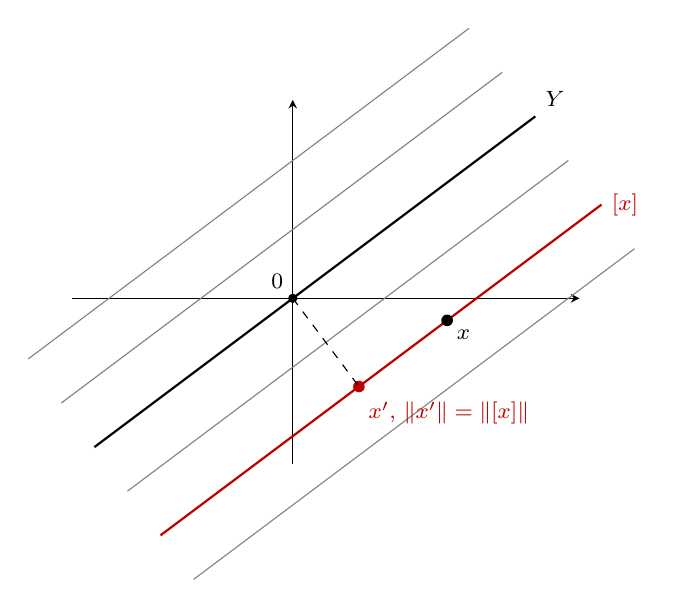
\begin{tikzpicture}[scale=1.4, >=stealth]
    \draw[->] (-2.0,0) -- (2.6,0) node[right] {};
    \draw[->] (0,-1.5) -- (0,1.8) node[above] {};
    % Y and parallel classes
    \draw[thick] (-1.8,-1.35) -- (2.2,1.65) node[above right, font=\footnotesize] {$Y$};
    \foreach \c in {-1.0,-0.5,0.5,1.5} {
        \draw[thin, gray] ({-1.8+\c*0.6},{-1.35-\c*0.8}) -- ({2.2+\c*0.6},{1.65-\c*0.8});
    }
    \draw[thick, red!75!black] ({-1.8+0.6},{-1.35-0.8}) -- ({2.2+0.6},{1.65-0.8}) node[right, font=\footnotesize] {$[x]$};
    % x on the red line
    \fill (1.4,-0.2) circle (1.5pt) node[below right, font=\footnotesize] {$x$};
    % closest point: foot of perpendicular from 0 onto red line (direction (4,3)/5, offset (0.6,-0.8))
    \fill[red!75!black] (0.6,-0.8) circle (1.5pt);
    \draw[dashed] (0,0) -- (0.6,-0.8);
    \node[below right, font=\footnotesize, red!75!black, yshift=-2pt] at (0.6,-0.8) {$x'$, $\|x'\| = \|[x]\|$};
    \fill (0,0) circle (1.2pt) node[above left, font=\footnotesize] {$0$};
\end{tikzpicture}
\end{center}
The classes are the parallel translates of $Y$; $\|[x]\|$ is the distance from the origin to the translate $[x]$, i.e.\ the norm of its closest point. With an inner product that point would be the foot of the perpendicular from $0$ (dashed); without one there is no perpendicular, the infimum need not be attained, and only the number $\inf \|x'\|$ is available. This is the same substitution of ``quotient'' for ``orthogonal complement'' as in \S\ref{subsec:quotient}.

\begin{proof}
$\|[x]\|$ is well defined: the set $\{\|x'\| : x' \in [x]\}$ is nonempty and bounded below by $0$, so its infimum is a real number $\ge 0$, and it depends only on the class, not on the representative $x$, since the set does. So $\|\cdot\| : X/Y \to \mathbb{R}_+$.

\textbf{Homogeneity.} Let $x_0 \in X$ and $a \in \mathbb{F}$. If $a = 0$ then $[a x_0] = [0] = Y$, and $\inf_{y \in Y} \|y\| = 0$ (attained at $y = 0$), which equals $|0|\,\|[x_0]\|$. If $a \ne 0$: since $Y$ is a subspace, $y \in Y$ iff $y/a \in Y$, so
\[
[a x_0] = \{ a x_0 + y : y \in Y \} = \{ a(x_0 + y') : y' \in Y \}
\]
(substitute $y = a y'$). Hence, by homogeneity of the norm on $X$ and the fact that constants pull out of infima,
\[
\|[a x_0]\| = \inf_{y' \in Y} \|a(x_0 + y')\| = \inf_{y' \in Y} |a|\,\|x_0 + y'\| = |a| \inf_{y' \in Y} \|x_0 + y'\| = |a|\, \|[x_0]\|.
\]
(Wu described this step as ``clear'' and left the writing to us.)

\textbf{Subadditivity.} Let $[x], [y] \in X/Y$; we show $\|[x + y]\| \le \|[x]\| + \|[y]\|$. Fix $\varepsilon > 0$. Since $\|[x]\|$ is the greatest lower bound of $\{\|x'\| : x' \in [x]\}$, the number $\|[x]\| + \varepsilon$ is not a lower bound, so there is $x_0 \in [x]$ with
\[
\|x_0\| \le \|[x]\| + \varepsilon;
\]
likewise there is $y_0 \in [y]$ with $\|y_0\| \le \|[y]\| + \varepsilon$. Now $x_0 + y_0 \in [x + y]$: indeed $(x_0 + y_0) - (x + y) = (x_0 - x) + (y_0 - y) \in Y$, both summands lying in $Y$. Therefore, by definition of the infimum and subadditivity of $\|\cdot\|$ on $X$,
\[
\|[x + y]\| \le \|x_0 + y_0\| \le \|x_0\| + \|y_0\| \le \|[x]\| + \|[y]\| + 2\varepsilon.
\]
Since $\varepsilon > 0$ was arbitrary, $\|[x+y]\| \le \|[x]\| + \|[y]\|$.

\textbf{Positivity.} Non-negativity was noted above. It remains to show that $\|[x]\| = 0$ implies $[x] = [0]$, i.e.\ $x \in Y$; this is where closedness of $Y$ is used. Suppose $\|[x]\| = \inf_{x' \in [x]} \|x'\| = 0$. Then there is a sequence $x_n \in [x]$ with $\|x_n\| \to 0$ (an infimum is approached by elements of the set). Since $x_n \in [x]$, we have $x_n - x \in Y$ for every $n$. And
\[
\bigl\| (x_n - x) - (-x) \bigr\| = \|x_n\| \to 0,
\]
so the sequence $\{x_n - x\} \subset Y$ converges to $-x$. Because $Y$ is closed, $-x \in Y$, hence $x \in Y$ (subspace), hence $[x] = [0]$.
\end{proof}

\begin{propbox}[The Quotient Seminorm; Closedness is Necessary]\boxlabel{prop:quotient-seminorm}
Let $Y$ be any linear subspace of a normed linear space $X$, closed or not. Then $\|[x]\| = \inf_{y \in Y}\|x + y\|$ is a seminorm on $X/Y$, and it is a norm if and only if $Y$ is closed.
\end{propbox}

\begin{proof}
Well-definedness, homogeneity and subadditivity were proved in Theorem~\ref{thm:quotient-norm} without using closedness, so $\|\cdot\|$ is a seminorm; if $Y$ is closed it is a norm by that theorem. Conversely, suppose $Y$ is not closed: there are $y_n \in Y$ with $y_n \to x$ for some $x \notin Y$. Then $x - y_n \in [x]$, so $\|[x]\| \le \|x - y_n\| \to 0$, i.e.\ $\|[x]\| = 0$, while $[x] \neq [0]$ because $x \notin Y$. So positivity fails. (Not stated in lecture.)
\end{proof}

% ============================================================================
% CHAPTER 4: INFINITE-DIMENSIONAL SPACES
% ============================================================================

\chapter{Infinite-Dimensional Spaces: $\ell^p$, $L^p$, and Compactness}

To produce normed spaces beyond $\mathbb{R}^n$ one needs the $p$-norms on sequences and functions to actually be norms, and the only nontrivial axiom is subadditivity (Minkowski's inequality), which rests on H\"older's inequality, which rests on Young's inequality. \ref{sec:young}--\ref{sec:completion-L1-sec} build that chain and the spaces $\ell^p$ and $L^p$ it produces; \ref{sec:noncompact} then uses them to exhibit the first structural difference between finite and infinite dimension. \ref{sec:young} is a recap of MATH 551 material given at the end of Lecture 3.

\section{Means and Young's Inequality}\label{sec:young}

\roadmark{Stage: norms}{Tools. The inequalities that make $\|\cdot\|_p$ a norm: Young, then H\"older (\ref{sec:holder}), then Minkowski (\ref{sec:minkowski}).}

\begin{propbox}[Cauchy--Schwarz in $\mathbb{R}^n$]\boxlabel{prop:cs}
For $x, y \in \mathbb{R}^n$, with $\|x\| = \bigl(x_1^2 + \cdots + x_n^2\bigr)^{1/2}$,
\[
|x \cdot y| \le \|x\|\, \|y\|.
\]
\end{propbox}

\begin{proof}
Recalled without proof in lecture; the standard argument is via the elementary inequality below or the discriminant of $t \mapsto \|x + ty\|^2$. See the MATH 551 notes.
\end{proof}

\begin{lembox}[{{Arithmetic--Geometric Mean, Two Variables}}]\boxlabel{lem:arithmetic-geometric-mean-two-variables}
For all real $a, b$, $2ab \le a^2 + b^2$; equivalently, for $a, b \ge 0$,
\[
\sqrt{ab} \le \tfrac{1}{2}(a + b).
\]
\end{lembox}

\begin{proof}
$0 \le (a - b)^2 = a^2 - 2ab + b^2$. For the second form, apply the first to $\sqrt{a}, \sqrt{b}$.
\end{proof}

The second form says that the geometric mean of two non-negative numbers is at most their arithmetic mean. Young's inequality is the weighted version: give $a$ weight $1 - \theta$ and $b$ weight $\theta$ in both averages.

\begin{lembox}[Young's Inequality]\boxlabel{lem:young}
For all $\theta \in [0, 1]$ and all $a, b \ge 0$,
\[
a^{1 - \theta}\, b^{\theta} \le (1 - \theta)\, a + \theta\, b.
\]
\end{lembox}

\begin{proof}
If $a = 0$ or $b = 0$ (with the convention $0^0 = 1$ at the endpoints $\theta \in \{0,1\}$), the left side is at most the right side directly; and for $\theta = 0$ or $\theta = 1$ both sides agree. So let $a, b > 0$ and $\theta \in (0,1)$. Since $\ln$ is increasing, the claim is equivalent to
\[
\ln\bigl(a^{1-\theta} b^{\theta}\bigr) \le \ln\bigl((1-\theta) a + \theta b\bigr),
\]
and since $\ln$ turns products into sums, the left side is $(1 - \theta) \ln a + \theta \ln b$. So the claim is
\[
(1 - \theta) \ln a + \theta \ln b \le \ln\bigl((1 - \theta) a + \theta b\bigr),
\]
which is concavity of $\ln$: the chord joining $(a, \ln a)$ and $(b, \ln b)$ lies below the graph. The point on the chord above $(1-\theta)a + \theta b$ has height $(1-\theta)\ln a + \theta \ln b$ by linearity of the chord, and the graph point above it has height $\ln\bigl((1-\theta)a + \theta b\bigr)$. (Concavity of $\ln$: $(\ln t)'' = -1/t^2 < 0$; see the MATH 551 notes for the chord characterization.)
\end{proof}

\begin{center}
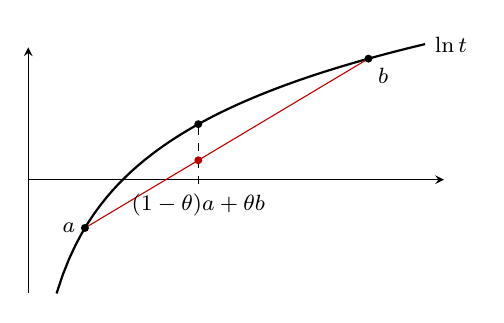
\begin{tikzpicture}[scale=1.2, >=stealth]
    \draw[->] (0,-1.2) -- (0,1.4);
    \draw[->] (0,0) -- (4.4,0);
    \draw[thick, domain=0.3:4.2, samples=60] plot (\x, {ln(\x)});
    \node[right, font=\footnotesize] at (4.2,1.43) {$\ln t$};
    \coordinate (A) at (0.6,{ln(0.6)});
    \coordinate (B) at (3.6,{ln(3.6)});
    \draw[red!75!black] (A) -- (B);
    \fill (A) circle (1.2pt) node[left, font=\footnotesize] {$a$};
    \fill (B) circle (1.2pt) node[below right, font=\footnotesize] {$b$};
    \coordinate (M) at (1.8,0);
    \draw[dashed] (1.8,-0.05) -- (1.8,{ln(1.8)});
    \fill (1.8,{ln(1.8)}) circle (1.2pt);
    \fill[red!75!black] (1.8,{ln(0.6)+ (1.8-0.6)/(3.6-0.6)*(ln(3.6)-ln(0.6))}) circle (1.2pt);
    \node[below, font=\footnotesize] at (1.8,-0.05) {$(1-\theta)a + \theta b$};
\end{tikzpicture}
\end{center}
Young's inequality is the case of the chord lying below the concave graph of $\ln$; the black dot is the graph value, the red dot the chord value.


% Lecture 4 (2026-09-10), last part
\section{H\"older's Inequality for Sequences}\label{sec:holder}

\roadmark{Stage: norms}{Tools. H\"older's inequality, from Young's.}

\begin{defbox}[The Sequence Space $\ell$ and the $p$-Norms]\boxlabel{def:sequence-space-l-p-norms}
Let $\ell$ denote the set of all infinite sequences $a = (a_1, a_2, \ldots)$ with $a_i \in \mathbb{F}$ ($= \mathbb{R}$ or $\mathbb{C}$). With termwise addition and scalar multiplication, $\ell$ is a linear space. For $a \in \ell$ define
\[
\|a\|_p = \Bigl( \sum_{i=1}^{\infty} |a_i|^p \Bigr)^{1/p} \quad (1 \le p < \infty), \qquad \|a\|_\infty = \sup_{i} |a_i|,
\]
with values in $[0, \infty]$.
\end{defbox}

\begin{rembox}\label{rem:holder}
On all of $\ell$ these are not norms: $\|a\|_p$ may be $+\infty$. They become norms on the subspace where they are finite, which is the space $\ell^p$ (to be defined once Minkowski's inequality is available). The name ``$p$-norm'' is used in advance, by abuse of language. For $\|\cdot\|_\infty$ the supremum, not the maximum, is needed: an infinite sequence need not attain its largest modulus.
\end{rembox}

\begin{defbox}[Conjugate Exponents]\boxlabel{def:conjugate-exponents}
For $1 \le p \le \infty$, the \textbf{conjugate exponent} $q$ is defined by
\[
\frac{1}{p} + \frac{1}{q} = 1, \qquad \text{i.e.\ } \frac{1}{q} = 1 - \frac{1}{p},
\]
with the conventions $1/\infty = 0$; so $q = \infty$ when $p = 1$, $q = 1$ when $p = \infty$, and $q = 2$ when $p = 2$. As $p$ ranges over $[1, \infty]$ so does $q$.
\end{defbox}

\begin{thmbox}[H\"older's Inequality for Sequences]\boxlabel{thm:holder-seq}
Let $1 \le p \le \infty$ and let $q$ be the conjugate exponent. For all $a = (a_i), b = (b_i) \in \ell$,
\[
\sum_{i=1}^{\infty} |a_i b_i| \;\le\; \|a\|_p\, \|b\|_q,
\]
with the convention $0 \cdot \infty = 0$ on the right.
\laxref{\S5.1, (19)}
\end{thmbox}

For $p = q = 2$ this is the Cauchy--Schwarz inequality (Proposition~\ref{prop:cs}) for infinite sequences.

\begin{proof}
\textbf{Case $p = 1$, $q = \infty$.} For every $i$, $|b_i| \le \sup_j |b_j| = \|b\|_\infty$, so
\[
\sum_{i} |a_i b_i| \le \sum_i |a_i|\, \|b\|_\infty = \|b\|_\infty\, \|a\|_1.
\]
The case $p = \infty$, $q = 1$ is the same with the roles of $a$ and $b$ exchanged.

\textbf{Case $1 < p < \infty$ (so $1 < q < \infty$).} (Lecture 5.)

\emph{Degenerate cases.} If $\|a\|_p = 0$ then every $a_i = 0$, the left side is $0$, and the inequality holds (with the convention $0 \cdot \infty = 0$ if $\|b\|_q = \infty$); likewise if $\|b\|_q = 0$. If $\|a\|_p = \infty$ or $\|b\|_q = \infty$ with the other factor nonzero, the right side is $+\infty$ and there is nothing to prove. So assume
\[
0 < \|a\|_p < \infty, \qquad 0 < \|b\|_q < \infty.
\]

\emph{Normalization.} Put
\[
a_i' = \frac{a_i}{\|a\|_p}, \qquad b_i' = \frac{b_i}{\|b\|_q}, \qquad a' = (a_i')_{i \ge 1},\ b' = (b_i')_{i \ge 1}.
\]
Then $\|a'\|_p = \|a\|_p / \|a\|_p = 1$ and $\|b'\|_q = 1$, by homogeneity of the $p$-norms (pull the positive constant out of the sum). Since $\sum_i |a_i b_i| = \|a\|_p \|b\|_q \sum_i |a_i' b_i'|$, it suffices to show
\[
\sum_{i=1}^\infty |a_i' b_i'| \le 1.
\]

\emph{Young's inequality termwise.} Set $1 - \theta = 1/p$ and $\theta = 1/q$; these are in $(0,1)$ and sum to $1$ by conjugacy. For each $i$, rewrite
\[
|a_i' b_i'| = |a_i'|\,|b_i'| = \bigl(|a_i'|^p\bigr)^{1/p} \bigl(|b_i'|^q\bigr)^{1/q} = \bigl(|a_i'|^p\bigr)^{1 - \theta} \bigl(|b_i'|^q\bigr)^{\theta}.
\]
Young's inequality (Lemma~\ref{lem:young}, for non-negative $|a_i'|^p$ and $|b_i'|^q$) gives
\[
|a_i' b_i'| \le (1 - \theta)\,|a_i'|^p + \theta\,|b_i'|^q = \frac{1}{p}|a_i'|^p + \frac{1}{q}|b_i'|^q.
\]

\emph{Sum.} Summing over $i$ (all terms non-negative, so the sums exist in $[0,\infty]$),
\[
\sum_{i=1}^\infty |a_i' b_i'| \le \frac{1}{p} \sum_{i=1}^\infty |a_i'|^p + \frac{1}{q} \sum_{i=1}^\infty |b_i'|^q = \frac{1}{p}\,\|a'\|_p^p + \frac{1}{q}\,\|b'\|_q^q = \frac{1}{p} + \frac{1}{q} = 1. \qedhere
\]
\end{proof}

\begin{rembox}\label{rem:holder-2}
The proof is an ``appropriate application of Young'': the normalization makes the right-hand side of Young sum to exactly $1$, and the exponents $p, q$ are chosen so that $|a_i'|^p$ and $|b_i'|^q$ are the two numbers being averaged. The finite-dimensional inequality $\sum_{i=1}^n |a_i b_i| \le \|a\|_p \|b\|_q$ on $\mathbb{R}^n$ or $\mathbb{C}^n$ is the special case of sequences with $a_i = b_i = 0$ for $i > n$. Nothing in the argument needed the sums to be finite in advance; that is why the theorem is stated on all of $\ell$.
\end{rembox}

% ============================================================================
% SECTION 13: MINKOWSKI
% ============================================================================

\section{Minkowski's Inequality and the Spaces $\ell^p$}\label{sec:minkowski}

\roadmark{Stage: norms}{Thread: completeness. The first infinite-dimensional Banach spaces.}

\subsection{Minkowski's Inequality}

\begin{thmbox}[Minkowski's Inequality for Sequences]\boxlabel{thm:minkowski-seq}
Let $1 \le p \le \infty$ and $a = (a_i), b = (b_i) \in \ell$. Then
\[
\|a + b\|_p \le \|a\|_p + \|b\|_p,
\]
where both sides are allowed to be $+\infty$.
\laxref{\S5.1, Thms~4--5}
\end{thmbox}

Wu's proof for $1 < p < \infty$ runs in two stages: a computation, valid as an inequality in $[0,\infty]$, followed by a cancellation that needs $\|a+b\|_p < \infty$; when that is not yet known, the computation is applied to truncations. The order below follows hers.

\begin{proof}[Proof of Theorem~\ref{thm:minkowski-seq}]
\textbf{Case $p = 1$.} $\sum_i |a_i + b_i| \le \sum_i (|a_i| + |b_i|) = \|a\|_1 + \|b\|_1$, by the termwise triangle inequality and addition of series of non-negative terms.

\textbf{Case $p = \infty$.} For every $i$, $|a_i + b_i| \le |a_i| + |b_i| \le \|a\|_\infty + \|b\|_\infty$; take the supremum over $i$.

\textbf{Case $1 < p < \infty$.} If $\|a\|_p = \infty$ or $\|b\|_p = \infty$, the right side is $+\infty$ and there is nothing to prove. So assume both are finite. Let $q = p/(p-1)$ be the conjugate exponent, so that
\begin{equation}\label{eq:mink-exp}
(p - 1)\, q = p, \qquad \frac{p}{q} = p - 1.
\end{equation}

\emph{Step 1: split one factor off.} Writing $|a_i + b_i|^p = |a_i + b_i|^{p-1}\,|a_i + b_i|$ and using $|a_i + b_i| \le |a_i| + |b_i|$,
\[
\|a + b\|_p^p = \sum_i |a_i + b_i|^{p-1}\,|a_i + b_i| \le \underbrace{\sum_i |a_i + b_i|^{p-1}\,|a_i|}_{\mathrm{I}} + \underbrace{\sum_i |a_i + b_i|^{p-1}\,|b_i|}_{\mathrm{II}},
\]
an inequality between elements of $[0, \infty]$.

\emph{Step 2: H\"older on each piece.} Apply Theorem~\ref{thm:holder-seq} to $\mathrm{I}$ with the exponent $q$ on the first factor and $p$ on the second:
\[
\mathrm{I} \le \Bigl( \sum_i \bigl(|a_i + b_i|^{p-1}\bigr)^{q} \Bigr)^{1/q} \Bigl( \sum_i |a_i|^p \Bigr)^{1/p} = \Bigl( \sum_i |a_i + b_i|^{p} \Bigr)^{1/q}\, \|a\|_p = \|a + b\|_p^{\,p/q}\, \|a\|_p,
\]
using $(p-1)q = p$ from \eqref{eq:mink-exp}. The same computation gives $\mathrm{II} \le \|a + b\|_p^{\,p/q}\, \|b\|_p$. Hence
\begin{equation}\label{eq:mink-pre}
\|a + b\|_p^p \le \|a + b\|_p^{\,p-1} \bigl( \|a\|_p + \|b\|_p \bigr).
\end{equation}

\emph{Step 3: cancel, if $\|a + b\|_p$ is finite.} If $\|a + b\|_p = 0$ there is nothing to prove. If $0 < \|a + b\|_p < \infty$, divide both sides of \eqref{eq:mink-pre} by $\|a + b\|_p^{\,p-1}$ to obtain $\|a + b\|_p \le \|a\|_p + \|b\|_p$. If $\|a + b\|_p = \infty$, \eqref{eq:mink-pre} reads $\infty \le \infty$ and cannot be cancelled.

\emph{Step 4: otherwise, truncate.} Let
\[
a^{(n)} = (a_1, \ldots, a_n, 0, 0, \ldots), \qquad b^{(n)} = (b_1, \ldots, b_n, 0, 0, \ldots).
\]
These are finitely supported, so all norms involved are finite sums, and Steps 1--3 apply to them:
\[
\Bigl( \sum_{i=1}^{n} |a_i + b_i|^p \Bigr)^{1/p} = \|a^{(n)} + b^{(n)}\|_p \le \|a^{(n)}\|_p + \|b^{(n)}\|_p \le \|a\|_p + \|b\|_p,
\]
the last step because a partial sum of non-negative terms is at most the full sum. The left side is increasing in $n$ and bounded by $\|a\|_p + \|b\|_p$; letting $n \to \infty$ gives $\|a + b\|_p \le \|a\|_p + \|b\|_p$. In particular $\|a + b\|_p < \infty$ whenever the right side is finite.
\end{proof}

\begin{lembox}[Minkowski for Finitely Supported Sequences]\boxlabel{lem:minkowski-finite}
Let $1 < p < \infty$ and let $a, b \in \ell$ have only finitely many nonzero terms. Then $\|a + b\|_p \le \|a\|_p + \|b\|_p$.
\end{lembox}

\begin{proof}
All three norms are finite sums, so Steps 1--3 of the proof of Theorem~\ref{thm:minkowski-seq} apply with no truncation: the computation gives \eqref{eq:mink-pre}, and the cancellation in Step 3 is legitimate.
\end{proof}

\begin{rembox}[Where the Finiteness is Used]\label{rem:where-finiteness-used}
A student asked what happens if the sums are infinite. The answer is in the structure above: Steps 1--2 are valid as inequalities in $[0,\infty]$ regardless, but Step 3 divides by $\|a+b\|_p^{\,p-1}$, and ``$\infty \le \infty \cdot C$'' cannot be cancelled to ``$\infty \le C$.'' The truncation makes every quantity finite, and monotone convergence of the partial sums then carries the inequality to the full series. This is a general pattern: prove the estimate in a setting where everything is finite, then pass to the limit through an increasing family. Minkowski fails for $0 < p < 1$: the same computation cannot be run because H\"older needs $q \ge 1$, and in fact $\|\cdot\|_p$ is then not subadditive: for $a = e_1$ and $b = e_2$, $\|a + b\|_p = 2^{1/p} > 2 = \|a\|_p + \|b\|_p$.
\end{rembox}

\subsection{The Spaces $\ell^p$}

\begin{defbox}[$\ell^p$]\boxlabel{def:lp}
For $1 \le p \le \infty$,
\[
\ell^p = \{ a \in \ell : \|a\|_p < \infty \}.
\]
(Also written $\ell_p$; both notations occur on the board.)
\laxref{\S5.1, example (b)}
\end{defbox}

\begin{propbox}[$\ell^p$ is a Normed Linear Space]\boxlabel{prop:lp-normed}
For $1 \le p \le \infty$, $\ell^p$ is a linear subspace of $\ell$, and $\|\cdot\|_p$ is a norm on it.
\laxref{\S5.1, Thm~4}
\end{propbox}

\begin{proof}
\emph{Subspace.} If $a, b \in \ell^p$ then $\|a + b\|_p \le \|a\|_p + \|b\|_p < \infty$ by Minkowski, so $a + b \in \ell^p$; and $\|ca\|_p = |c|\,\|a\|_p < \infty$ (below), so $ca \in \ell^p$; $0 \in \ell^p$.

\emph{Positivity.} $\|a\|_p \ge 0$ as a sum (or supremum) of non-negative numbers, and $\|a\|_p = 0$ iff every $|a_i|^p = 0$ (resp.\ every $|a_i| = 0$) iff $a = 0$.

\emph{Homogeneity.} For $p < \infty$, $\|ca\|_p = \bigl(\sum_i |c|^p |a_i|^p\bigr)^{1/p} = |c|\,\|a\|_p$; for $p = \infty$, $\sup_i |c a_i| = |c| \sup_i |a_i|$.

\emph{Subadditivity.} Theorem~\ref{thm:minkowski-seq}.
\end{proof}

\begin{rembox}\label{rem:minkowski}
$\ell^p$ is the first genuinely infinite-dimensional normed space in the course: it contains the linearly independent sequences $e_1 = (1,0,0,\ldots)$, $e_2 = (0,1,0,\ldots)$, \dots. Unlike the norms $\|\cdot\|_p$ on $\mathbb{R}^n$, the spaces $\ell^p$ for different $p$ are different sets, and their norms are not equivalent where both are defined.
\end{rembox}

\begin{propbox}[Nesting of the $\ell^p$ Spaces]\boxlabel{prop:lp-nested}
Let $1 \le p < q \le \infty$.
\begin{enumerate}[label=(\alph*)]
    \item $\|a\|_q \le \|a\|_p$ for every $a \in \ell$; in particular $\ell^p \subset \ell^q$.
    \item The inclusion is strict: $\ell^p \neq \ell^q$.
    \item On $\ell^p$, the norms $\|\cdot\|_p$ and $\|\cdot\|_q$ are not equivalent.
\end{enumerate}
\end{propbox}

\begin{proof}
(Not covered in lecture.) (a) If $a = 0$ or $\|a\|_p = \infty$ there is nothing to prove; otherwise, by homogeneity, we may assume $\|a\|_p = 1$. Then $|a_i| \le 1$ for every $i$, a single term being at most the sum. If $q = \infty$, $\|a\|_\infty = \sup_i |a_i| \le 1$. If $q < \infty$, then $|a_i|^q \le |a_i|^p$ because $|a_i| \le 1$ and $q > p$, so $\|a\|_q^q \le \sum_i |a_i|^p = 1$.

(b) If $q < \infty$, let $a_i = i^{-1/p}$: then $\sum_i |a_i|^p = \sum_i 1/i = \infty$, while $\sum_i |a_i|^q = \sum_i i^{-q/p} < \infty$ because $q/p > 1$. If $q = \infty$, the constant sequence $(1, 1, \ldots)$ lies in $\ell^\infty \setminus \ell^p$.

(c) For $s_n = e_1 + \cdots + e_n$ we have $\|s_n\|_p = n^{1/p}$ and $\|s_n\|_q = n^{1/q}$ (with $1/\infty = 0$), so $\|s_n\|_p / \|s_n\|_q = n^{1/p - 1/q} \to \infty$, and no constant $C$ gives $\|a\|_p \le C\|a\|_q$ on $\ell^p$.
\end{proof}

\begin{center}
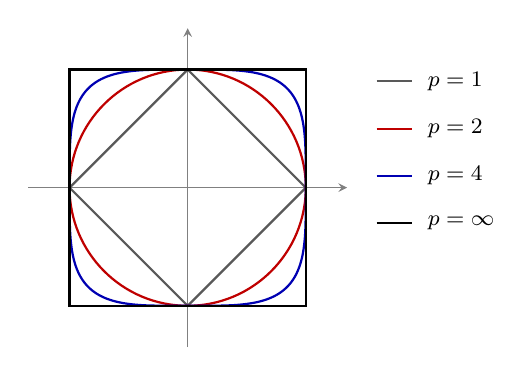
\begin{tikzpicture}[scale=1.5, >=stealth]
    \draw[->, gray] (-1.35,0) -- (1.35,0);
    \draw[->, gray] (0,-1.35) -- (0,1.35);
    \draw[thick, gray!70!black] (1,0) -- (0,1) -- (-1,0) -- (0,-1) -- cycle;
    \draw[thick, red!75!black] (0,0) circle (1);
    \draw[thick, blue!70!black, smooth, domain=0.5:360.5, samples=181]
        plot ({sign(cos(\x))*abs(cos(\x))^(0.5)}, {sign(sin(\x))*abs(sin(\x))^(0.5)});
    \draw[thick] (-1,-1) rectangle (1,1);
    \foreach \y/\st/\lab in {0.9/{gray!70!black}/{$p = 1$}, 0.5/{red!75!black}/{$p = 2$}, 0.1/{blue!70!black}/{$p = 4$}, -0.3/{black}/{$p = \infty$}} {
        \draw[thick, \st] (1.6,\y) -- (1.9,\y);
        \node[anchor=west] at (1.95,\y) {\lab};
    }
\end{tikzpicture}
\end{center}
The unit balls $\{\|x\|_p \le 1\}$ in $\mathbb{R}^2$ increase with $p$; this is (a) for vectors with two nonzero entries. All four norms are equivalent on $\mathbb{R}^2$ (Theorem~\ref{prop:norms-equiv}), and (c) is the statement that this fails on $\ell^p$.

\subsection{Completeness of $\ell^p$}

\begin{thmbox}[$\ell^p$ is a Banach Space]\boxlabel{thm:lp-complete}
For $1 \le p \le \infty$, $(\ell^p, \|\cdot\|_p)$ is complete.
\laxref{\S5.1, examples (a)--(b)}
\end{thmbox}

\begin{notebox}[Notation for the Proof]\label{note:notation-proof-2}
A sequence in $\ell^p$ is a sequence of sequences. Write the $n$-th term as
\[
a^{(n)} = \bigl( a^{(n)}_1, a^{(n)}_2, a^{(n)}_3, \ldots \bigr) \in \ell^p,
\]
so the superscript indexes the term of the sequence in $\ell^p$ and the subscript the coordinate. Wu also used truncations $a^{(n,k)} = (a^{(n)}_1, \ldots, a^{(n)}_k) \in \mathbb{F}^k$.
\end{notebox}

\begin{proof}
The proof follows the plan Wu stated for every completeness argument: \emph{first find the candidate for the limit, then prove convergence to it}. Take $p < \infty$ first.

Let $\{a^{(n)}\}_{n \ge 1}$ be Cauchy in $\ell^p$: for every $\varepsilon > 0$ there is $N$ such that
\begin{equation}\label{eq:lp-cauchy}
\sum_{i=1}^{\infty} \bigl| a^{(n)}_i - a^{(m)}_i \bigr|^p < \varepsilon^p \qquad \text{for all } n, m \ge N.
\end{equation}

\textbf{Step 1: The candidate, through truncations.} For $k \in \mathbb{N}$ let
\[
a^{(n,k)} = \bigl( a^{(n)}_1, \ldots, a^{(n)}_k \bigr) \in \mathbb{F}^k,
\]
and give $\mathbb{F}^k$ the norm $\|(c_1, \ldots, c_k)\|_p = \bigl( \sum_{i=1}^k |c_i|^p \bigr)^{1/p}$. Fix $k$. A partial sum of non-negative terms is at most the full sum, so
\[
\bigl\| a^{(n,k)} - a^{(m,k)} \bigr\|_p = \Bigl( \sum_{i=1}^{k} \bigl| a^{(n)}_i - a^{(m)}_i \bigr|^p \Bigr)^{1/p} \le \bigl\| a^{(n)} - a^{(m)} \bigr\|_p \xrightarrow[n, m \to \infty]{} 0 .
\]
So $\{a^{(n,k)}\}_n$ is Cauchy in $(\mathbb{F}^k, \|\cdot\|_p)$, which is complete (Corollary~\ref{cor:findim-complete}); hence there is $a^{(k)} \in \mathbb{F}^k$ with $\|a^{(n,k)} - a^{(k)}\|_p \to 0$ as $n \to \infty$.

The limits are consistent. The first $k$ coordinates of $a^{(n,k+1)}$ form $a^{(n,k)}$, and convergence in $\mathbb{F}^{k+1}$ implies convergence of each coordinate (a single term is at most the sum). So the first $k$ coordinates of $a^{(k+1)}$ are the limits of the coordinates of $a^{(n,k)}$, which by uniqueness of limits are the coordinates of $a^{(k)}$:
\[
a^{(k+1)} = \bigl( a^{(k)},\, a_{k+1} \bigr) \qquad \text{for some scalar } a_{k+1}.
\]
Hence there is a single sequence $a = (a_1, a_2, \ldots) \in \ell$ with $a^{(k)} = (a_1, \ldots, a_k)$ for every $k$; in particular $a^{(n)}_i \to a_i$ as $n \to \infty$ for each $i$. This is the candidate. Nothing has been proved about it yet: it is not known that $a \in \ell^p$, nor that $a^{(n)} \to a$ in $\|\cdot\|_p$.

\textbf{Step 2: A uniform tail estimate.} Fix $\varepsilon > 0$ and $N$ as in \eqref{eq:lp-cauchy}, and fix $n \ge N$. For any $k \in \mathbb{N}$ and any $m \ge N$, a partial sum is at most the full sum, so
\[
\sum_{i=1}^{k} \bigl| a^{(n)}_i - a^{(m)}_i \bigr|^p \le \sum_{i=1}^{\infty} \bigl| a^{(n)}_i - a^{(m)}_i \bigr|^p < \varepsilon^p.
\]
The left side is $\|a^{(n,k)} - a^{(m,k)}\|_p^p$, a \emph{finite} sum of $k$ terms, each of which converges as $m \to \infty$ by Step 1 (to $|a^{(n)}_i - a_i|^p$, by continuity of $t \mapsto |t|^p$). A limit of finitely many convergent terms is the sum of the limits, and non-strict inequalities survive limits, so
\[
\sum_{i=1}^{k} \bigl| a^{(n)}_i - a_i \bigr|^p \le \varepsilon^p \qquad \text{for every } k \in \mathbb{N} \text{ and every } n \ge N.
\]
The left side is increasing in $k$ and bounded by $\varepsilon^p$ independently of $k$, so its limit exists and
\begin{equation}\label{eq:lp-tail}
\sum_{i=1}^{\infty} \bigl| a^{(n)}_i - a_i \bigr|^p \le \varepsilon^p, \qquad \text{i.e.} \qquad \|a^{(n)} - a\|_p \le \varepsilon \qquad \text{for all } n \ge N.
\end{equation}

\textbf{Step 3: Conclusion.} By \eqref{eq:lp-tail} with $n = N$, $a - a^{(N)} \in \ell^p$; since $a^{(N)} \in \ell^p$ and $\ell^p$ is a linear space (Proposition~\ref{prop:lp-normed}), $a = a^{(N)} + (a - a^{(N)}) \in \ell^p$. And \eqref{eq:lp-tail} says precisely that $\|a^{(n)} - a\|_p \to 0$ as $n \to \infty$. So the Cauchy sequence converges in $\ell^p$.

\textbf{The case $p = \infty$.} The same three steps with sums replaced by suprema. Cauchy means $\sup_i |a^{(n)}_i - a^{(m)}_i| < \varepsilon$ for $n, m \ge N$; each coordinate is Cauchy, giving $a_i = \lim_n a^{(n)}_i$; for fixed $i$ and $n \ge N$, $|a^{(n)}_i - a^{(m)}_i| < \varepsilon$ for all $m \ge N$, and letting $m \to \infty$ gives $|a^{(n)}_i - a_i| \le \varepsilon$; taking the supremum over $i$ gives $\|a^{(n)} - a\|_\infty \le \varepsilon$ for $n \ge N$, whence $a \in \ell^\infty$ and $a^{(n)} \to a$.
\end{proof}

\begin{rembox}[The Two Limits]\label{rem:two-limits}
The delicate point is Step 2, and it produced the longest discussion in lecture. Two limits are involved: $m \to \infty$ (to replace $a^{(m)}$ by the candidate $a$) and $k \to \infty$ (to pass from partial sums to the full series). A student proposed handling the infinite sum directly as a limit of partial sums and choosing, for each $k$, an $n$ large enough. That does not work: the $n$ obtained depends on $k$, and as $k \to \infty$ it may go to infinity with it, so nothing is proved for the full series with a single $n$. The proof avoids this by using the Cauchy condition in its full form \eqref{eq:lp-cauchy} --- with the \emph{infinite} sum and $N$ independent of everything else --- and only then truncating to a finite sum, where $m \to \infty$ can be taken termwise, and finally sending $k \to \infty$ through a monotone bounded sequence. The order matters: truncate, then $m \to \infty$, then $k \to \infty$, with $n \ge N$ fixed throughout. Interchanging limits requires justification; when two are present, arrange for one of them to be a finite sum.
\end{rembox}

\begin{rembox}[The Coordinate Formulation]\label{rem:coordinate-formulation}
Step 1 can be shortened by working with one coordinate at a time. Fix a coordinate $i$. A single term of a series of non-negative numbers is at most the sum, so
\[
\bigl| a^{(n)}_i - a^{(m)}_i \bigr| \le \Bigl( \sum_{j=1}^\infty \bigl| a^{(n)}_j - a^{(m)}_j \bigr|^p \Bigr)^{1/p} = \|a^{(n)} - a^{(m)}\|_p.
\]
Hence $\{a^{(n)}_i\}_{n \ge 1}$ is a Cauchy sequence of scalars, and since $\mathbb{R}$ and $\mathbb{C}$ are complete it converges:
\[
a_i := \lim_{n \to \infty} a^{(n)}_i \qquad (i = 1, 2, \ldots).
\]
Put $a = (a_1, a_2, \ldots) \in \ell$. This is the candidate. Nothing has been proved about it yet: it is not known that $a \in \ell^p$, nor that $a^{(n)} \to a$ in $\|\cdot\|_p$; only that each coordinate converges.
As Wu noted at the end of the lecture, the two formulations are the same thing: convergence in $\mathbb{F}^k$ is coordinatewise convergence, and only the coordinates are used afterwards. A student's example of $e_1, e_2, e_1, e_2, \ldots$ (alternating) was raised as a worry for coordinatewise limits; it is not Cauchy in $\ell^p$ ($\|e_1 - e_2\|_p = 2^{1/p}$ does not go to $0$), so it is not a counterexample to anything.
\end{rembox}

\begin{rembox}[Comparison with Lax]\label{rem:comparison-lax-4}
Three differences of route in \ref{sec:holder}--\ref{sec:minkowski}. Lax states H\"older's inequality without proof, referring to Courant; here it is proved from Young's inequality (Lemma~\ref{lem:young}). Lax obtains Minkowski's inequality from the \emph{duality formula} $\|x\|_p = \max_{\|u\|_q = 1} |(x, u)|$ with $(x,u) = \sum_j a_j c_j$ (his Theorem~5): a maximum of sums is at most a sum of maxima, so subadditivity is immediate once the formula is known, and the formula itself rests on the equality case of H\"older. Wu's route (Theorem~\ref{thm:minkowski-seq}) avoids the equality case at the price of the truncation argument. The duality formula is the first appearance of the dual-space theme that returns in Lax's Chapter~8. Finally, Lax asserts the completeness of $\ell^p$ and $\ell^\infty$ without proof (examples (a)--(b)); Theorem~\ref{thm:lp-complete} proves it.
\end{rembox}

% ============================================================================
% SECTION 14: THE FUNCTION SPACES L^p
% ============================================================================

\section{The Function Spaces $L^p(\Omega)$}\label{sec:completion-L1-sec}

\roadmark{Stage: norms}{Thread: completeness. Function spaces; $L^p$ as the completion of $C[a,b]$.}

\subsection{Definition and the Integral Inequalities}

The second way to go to infinite dimensions is to index by a continuum: a function $f$ on $[a, b]$ assigns to each $x$ a value $f(x)$, and functions can be added and scaled, so the functions on $[a,b]$ form a linear space. The analogue of $\sum_i |a_i|^p$ is an integral.

\begin{rembox}[The Integral as a Sum]\label{rem:integral-sum}
For continuous $f$ on $[a,b]$ and a partition $a = x_0 < x_1 < \cdots < x_n = b$ with $\Delta x_i = x_{i+1} - x_i$,
\[
\int_a^b |f(x)|\, dx \;\approx\; \sum_{i=0}^{n-1} |f(x_i)|\, \Delta x_i,
\]
the Riemann sum, which improves as the partition is refined. So $\int |f|^p$ is the continuum version of $\sum |a_i|^p$, with $f(x_i)$ in place of $a_i$ and the widths $\Delta x_i$ as weights.
\begin{center}
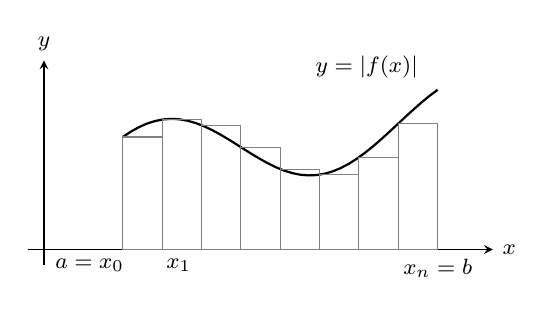
\begin{tikzpicture}[scale=1.0, >=stealth]
    \draw[->] (-0.7,0) -- (5.2,0) node[right] {$x$};
    \draw[->] (-0.5,-0.2) -- (-0.5,2.4) node[above] {$y$};
    \draw[thick, domain=0.5:4.5, samples=40] plot (\x, {1.0 + 0.5*sin(\x*90) + 0.15*\x});
    \node[above, font=\footnotesize] at (3.6,2.05) {$y = |f(x)|$};
    \foreach \i in {0,...,7} {
        \pgfmathsetmacro{\xa}{0.5 + \i*0.5}
        \pgfmathsetmacro{\ya}{1.0 + 0.5*sin(\xa*90) + 0.15*\xa}
        \draw[thin, gray] (\xa,0) rectangle ({\xa+0.5},\ya);
    }
    \node[below, font=\footnotesize, anchor=north east, xshift=4pt] at (0.5,0) {$a = x_0$};
    \node[below, font=\footnotesize, anchor=north west, xshift=-2pt] at (1.0,0) {$x_1$};
    \node[below, font=\footnotesize] at (4.5,0) {$x_n = b$};
\end{tikzpicture}
\end{center}
\end{rembox}

\begin{defbox}[{{$L^p(\Omega)$, $L^\infty(\Omega)$ --- working definition}}]\boxlabel{def:Lp}
Let $\Omega \subset \mathbb{R}^n$ be a domain. For $1 \le p < \infty$,
\[
L^p(\Omega) = \Bigl\{ f \text{ measurable on } \Omega : \|f\|_{L^p} := \Bigl( \int_\Omega |f(x)|^p\, dx \Bigr)^{1/p} < \infty \Bigr\},
\]
and
\[
L^\infty(\Omega) = \Bigl\{ f \text{ bounded on } \Omega : \|f\|_{L^\infty} := \sup_{x \in \Omega} |f(x)| < \infty \Bigr\}.
\]
$\|f\|_{L^p}$ is also written $\|f\|_p$.
\laxref{\S5.1, example (f)}
\end{defbox}

\begin{rembox}[What ``Integrable'' Means Here]\label{rem:what-integrable-means-here}
On the board the definition read ``$f$ integrable on $\Omega$'', and Wu deliberately left ``integrable'' unspecified. Rigorously the condition is that $f$ be Lebesgue measurable with finite integral of $|f|^p$; for $p > 1$ this does not require $\int_\Omega |f| < \infty$ ($1/x$ on $(1, \infty)$ is in $L^2$ but not in $L^1$). Functions agreeing outside a set of measure zero are identified, and $\|f\|_{L^\infty}$ is the essential supremum; without the identification, positivity of the norm fails ($f = 0$ except at one point has $\|f\|_p = 0$). Since MATH 551 is not a prerequisite for this course, she asked us to take ``integrable'' as ``anything you will meet,'' with continuous functions as the safe case (continuous on a compact $\Omega$ implies Riemann integrable), and said the theory could be made rigorous later. The full treatment --- Lebesgue integral, $L^p$, H\"older, Minkowski, Riesz--Fischer, dominated and monotone convergence, Fatou --- is in the MATH 551 notes, Chapters on Lebesgue integration and $L^p$ spaces, and that is the version to rely on. (For those without it: chapter 2 of the posted reference notes.)
\end{rembox}

\begin{thmbox}[H\"older's Inequality for Functions]\boxlabel{thm:holder-fn}
Let $1 \le p \le \infty$ and $q$ its conjugate. For $f \in L^p(\Omega)$, $g \in L^q(\Omega)$,
\[
\int_\Omega |f(x) g(x)|\, dx \le \|f\|_{L^p}\, \|g\|_{L^q}.
\]
\end{thmbox}

\begin{proof}
Not proved in lecture; ``the same idea, exactly'' as Theorem~\ref{thm:holder-seq}, with the integral in place of the sum: normalize, apply Young pointwise, integrate. A full proof is in the MATH 551 notes, Chapter \emph{$L^p$ Spaces}, subsection \emph{H\"older's Inequality} (Theorem: H\"older's Inequality).
\end{proof}

\begin{thmbox}[Minkowski's Inequality for Functions]\boxlabel{thm:minkowski-fn}
For $1 \le p \le \infty$ and $f, g \in L^p(\Omega)$,
\[
\|f + g\|_{L^p} \le \|f\|_{L^p} + \|g\|_{L^p}.
\]
\end{thmbox}

\begin{proof}
Not proved in lecture; as for Theorem~\ref{thm:minkowski-seq}, with the same truncation issue handled by first assuming $\|f+g\|_p < \infty$ (which follows from $|f+g|^p \le 2^{p-1}(|f|^p + |g|^p)$). A full proof is in the MATH 551 notes, Chapter \emph{$L^p$ Spaces}, subsection \emph{$L^p$ is a Normed Linear Space} (Theorem: Minkowski's Inequality, with corollaries for finite sums and series).
\end{proof}

\subsection{Completeness and Density}

\begin{thmbox}[$L^p(\Omega)$ and $L^\infty(\Omega)$ are Banach Spaces]\boxlabel{thm:Lp-complete}
For $1 \le p \le \infty$, $(L^p(\Omega), \|\cdot\|_{L^p})$ is a complete normed linear space.
\end{thmbox}

\begin{proof}
Deferred: Wu skipped the proof because it needs real-analysis tools (a candidate limit must be built from an almost-everywhere convergent subsequence, and monotone/dominated convergence used to close the argument). The plan is the same as for $\ell^p$ --- find the candidate, then prove convergence --- but the candidate is harder to produce. The theorem is Riesz--Fischer; a full proof is in the MATH 551 notes, Chapter \emph{$L^p$ Spaces}, subsection \emph{The Riesz--Fischer Theorem}.
\end{proof}

\begin{thmbox}[Density of Smooth Functions]\boxlabel{thm:density}
For $1 \le p < \infty$, $C_c^\infty(\Omega)$, the smooth functions with compact support in $\Omega$, is dense in $L^p(\Omega)$: for every $f \in L^p(\Omega)$ and $\varepsilon > 0$ there is $\varphi \in C_c^\infty(\Omega)$ with $\|f - \varphi\|_{L^p} < \varepsilon$.
\end{thmbox}

\begin{proof}
Deferred. Wu said she would look for a proof that avoids heavy measure theory and present it next lecture if one is available. (The MATH 551 notes, Chapter \emph{$L^p$ Spaces}, subsection \emph{Density and Separability}, prove that simple functions, step functions, and compactly supported continuous functions are dense in $L^p$ for $1 \le p < \infty$; smoothing by convolution with a $C^\infty$ bump takes it the rest of the way to $C_c^\infty$.)
\end{proof}

\begin{propbox}[Continuous Functions are Not Dense in $L^\infty$]\boxlabel{prop:C-not-dense}
$C(\Omega)$ is not dense in $L^\infty(\Omega)$.
\end{propbox}

\begin{proof}
Take $\Omega = [0,1]$ and the step function $f = \chi_{[1/2, 1]}$, i.e.\ $f(x) = 0$ for $x < 1/2$ and $f(x) = 1$ for $x \ge 1/2$; $f$ is bounded, so $f \in L^\infty[0,1]$. We claim $\|f - g\|_{L^\infty} \ge 1/2$ for every $g \in C[0,1]$, so no sequence of continuous functions converges to $f$ in $L^\infty$. Suppose instead $\|f - g\|_{L^\infty} = \sup_x |f(x) - g(x)| < 1/2$ for some continuous $g$. Then for $x < 1/2$, $|g(x)| = |f(x) - g(x)| < 1/2$, and for $x \ge 1/2$, $|g(x) - 1| < 1/2$, so $g(x) > 1/2$. By continuity of $g$ at $1/2$, $g(1/2) = \lim_{x \to 1/2^-} g(x) \le 1/2$, while $g(1/2) > 1/2$ from the second condition: a contradiction. (With the Lebesgue definition of $L^\infty$ the same argument works after replacing ``for all $x$'' by ``for almost every $x$'' and using that a continuous function satisfying a strict inequality almost everywhere on an interval satisfies the non-strict one everywhere on it.)

Alternatively, as Wu suggested: $C[0,1]$ with the supremum norm is complete (Theorem~\ref{thm:Cab-banach}), hence a closed subspace of $L^\infty[0,1]$ (Lemma~\ref{lem:complete-closed}), and a closed proper subspace is not dense; $f$ above shows the inclusion is proper.
\end{proof}

\begin{rembox}\label{rem:completion-L1-sec}
The failure at $p = \infty$ is the first sign that $L^\infty$ behaves differently from the other $L^p$: uniform approximation cannot smooth out a jump. The pattern ``true for $1 \le p < \infty$, false for $p = \infty$'' will recur, e.g.\ in identifying dual spaces.
\end{rembox}

\subsection{The Completion of $C[a,b]$ in the $L^p$ Norm}\label{subsec:completion-L1}

\begin{lembox}[A Vanishing Integral]\boxlabel{lem:vanishing-int}
Let $\alpha < \beta$ and let $h : [\alpha,\beta] \to [0,\infty)$ be continuous with $\int_\alpha^\beta h(x)\,dx = 0$. Then $h(x) = 0$ for all $x \in [\alpha,\beta]$.
\end{lembox}

\begin{proof}
(HW3, Problem 1.) Suppose $h(x_0) = \eta > 0$ for some $x_0 \in [\alpha,\beta]$. By continuity there is $\delta > 0$ with $h(x) > \eta/2$ for all $x \in I := [x_0 - \delta, x_0 + \delta] \cap [\alpha,\beta]$. Since $\alpha < \beta$, $I$ is an interval of some length $\ell > 0$. As $h \geq 0$ on $[\alpha,\beta]$,
\[\int_\alpha^\beta h \geq \int_I h \geq \ell \cdot \frac{\eta}{2} > 0,\]
a contradiction.
\end{proof}

\begin{lembox}[H\"older's Inequality for Continuous Functions]\boxlabel{lem:holder-cont}
Let $1 < p < \infty$ and $q = p/(p-1)$, so that $\frac1p + \frac1q = 1$. For $u, v \in C([a,b])$,
\[\int_a^b |u(x)\,v(x)|\,dx \leq \Bigl( \int_a^b |u|^p \Bigr)^{1/p} \Bigl( \int_a^b |v|^q \Bigr)^{1/q}.\]
\end{lembox}

\begin{proof}
(HW3, Problem 1.) Write $A = (\int_a^b |u|^p)^{1/p}$ and $B = (\int_a^b |v|^q)^{1/q}$. If $A = 0$, then $|u|^p \equiv 0$ by Lemma~\ref{lem:vanishing-int}, so $u \equiv 0$ and both sides vanish; likewise if $B = 0$. Otherwise put $U = u/A$ and $V = v/B$, so that $\int_a^b |U|^p = \int_a^b |V|^q = 1$. Young's inequality from class, $s^{1-\theta} t^{\theta} \leq (1-\theta)\,s + \theta\, t$ for $s, t \geq 0$ and $\theta \in [0,1]$, applied at each $x \in [a,b]$ with $s = |U(x)|^p$, $t = |V(x)|^q$, $\theta = 1/q$ (so $1 - \theta = 1/p$), gives
\[|U(x)|\,|V(x)| \leq \frac1p\,|U(x)|^p + \frac1q\,|V(x)|^q.\]
Both sides are continuous in $x$; integrating over $[a,b]$ (monotonicity and linearity of the integral),
\[\int_a^b |UV| \leq \frac1p + \frac1q = 1,\]
and multiplying by $AB$ gives the claim.
\end{proof}

\begin{propbox}[{{$L^p[a,b]$ as a Completion}}]\boxlabel{prop:completion-L1}
Let $1 \le p < \infty$ and let $X = C[a,b]$, the continuous functions on $[a,b]$, with the norm
\[
\|f\|_p = \Bigl( \int_a^b |f(x)|^p\, dx \Bigr)^{1/p}.
\]
Then $(X, \|\cdot\|_p)$ is a normed linear space, it is not complete, and its completion is $L^p[a,b]$.
\laxref{\S5.1, example (f)}
\end{propbox}

\begin{proof}
(HW3, Problem 1.) 
Throughout, $\mathbb{F}$ denotes the scalar field ($\mathbb{R}$ or $\mathbb{C}$), $a < b$, and $X = C([a,b])$ is the space of continuous functions $f : [a,b] \to \mathbb{F}$ with pointwise operations; $X$ is a linear space (Theorem~\ref{thm:Cab-banach}, Part 1). Integrals of continuous functions are Riemann integrals. We show that $(X, \|\cdot\|_p)$ is a normed linear space, that it is \emph{not} complete, and that its completion is $L^p([a,b])$.

\textbf{Part 1: $\|\cdot\|_p$ is a norm on $X$.}

\emph{Well defined.} For $f \in X$ the function $|f|^p$ is continuous on $[a,b]$, as a composition of continuous maps, hence Riemann integrable with $\int_a^b |f|^p \in [0,\infty)$. So $\|f\|_p$ is a well-defined non-negative real number.

\emph{Positivity.} $\|f\|_p \geq 0$. If $\|f\|_p = 0$, then $\int_a^b |f|^p = 0$, so $|f|^p \equiv 0$ by Lemma~\ref{lem:vanishing-int}, i.e.\ $f = 0$. Conversely $\|0\|_p = 0$.

\emph{Homogeneity.} For $c \in \mathbb{F}$,
\[\|cf\|_p = \Bigl( \int_a^b |c|^p\,|f|^p \Bigr)^{1/p} = \Bigl( |c|^p \int_a^b |f|^p \Bigr)^{1/p} = |c|\,\|f\|_p.\]

\emph{Triangle inequality.} Let $f, g \in X$. If $p = 1$, integrate the pointwise inequality $|f + g| \leq |f| + |g|$. Let $1 < p < \infty$ and $q = p/(p-1)$, so that $(p - 1)\,q = p$. If $\|f + g\|_p = 0$ there is nothing to prove, so assume $\|f + g\|_p > 0$. Pointwise,
\[|f + g|^p = |f + g|^{p-1}\,|f + g| \leq |f|\,|f + g|^{p-1} + |g|\,|f + g|^{p-1},\]
and every function here is continuous. Integrating, and applying Lemma~\ref{lem:holder-cont} to each term with $u = |f|$ (respectively $u = |g|$) and $v = |f + g|^{p-1}$,
\[\|f + g\|_p^p \leq \bigl( \|f\|_p + \|g\|_p \bigr) \Bigl( \int_a^b |f + g|^{(p-1)q} \Bigr)^{1/q} = \bigl( \|f\|_p + \|g\|_p \bigr)\, \|f + g\|_p^{\,p/q}.\]
Since $0 < \|f + g\|_p < \infty$ and $p - p/q = 1$, dividing by $\|f + g\|_p^{\,p/q}$ gives $\|f + g\|_p \leq \|f\|_p + \|g\|_p$.

Hence $(X, \|\cdot\|_p)$ is a normed linear space.

\textbf{Part 2: $(X, \|\cdot\|_p)$ is not complete.} Let $c = (a+b)/2$ and fix $N_0 \in \mathbb{N}$ with $1/N_0 < b - c$. For $n \geq N_0$ define
\[f_n(x) = \begin{cases} 0, & a \leq x \leq c, \\ n(x - c), & c \leq x \leq c + \frac1n, \\ 1, & c + \frac1n \leq x \leq b. \end{cases}\]
Each $f_n$ is continuous, since the formulas agree at $x = c$ and at $x = c + \frac1n$, and $0 \leq f_n \leq 1$.

\emph{$\{f_n\}$ is Cauchy.} Let $N \geq N_0$ and $m, n \geq N$. Both $f_m$ and $f_n$ vanish on $[a, c]$ and both equal $1$ on $[c + \frac1N, b]$, because $c + \frac1m \leq c + \frac1N$ and $c + \frac1n \leq c + \frac1N$. So $f_m - f_n = 0$ outside $[c, c + \frac1N]$, and $|f_m - f_n| \leq 1$ everywhere since both take values in $[0,1]$. Hence
\[\|f_m - f_n\|_p^p = \int_c^{c + 1/N} |f_m - f_n|^p \leq \frac1N, \qquad \text{i.e.} \qquad \|f_m - f_n\|_p \leq N^{-1/p} \xrightarrow[N \to \infty]{} 0.\]

\emph{$\{f_n\}$ has no limit in $X$.} Suppose $f \in X$ with $\|f_n - f\|_p \to 0$.
\begin{itemize}
\item On $[a, c]$ we have $f_n = 0$, so for every $n \geq N_0$,
\[\int_a^c |f|^p = \int_a^c |f_n - f|^p \leq \|f_n - f\|_p^p.\]
The left side does not depend on $n$ and the right side tends to $0$, so $\int_a^c |f|^p = 0$, and Lemma~\ref{lem:vanishing-int} gives $f = 0$ on $[a, c]$. In particular $f(c) = 0$.
\item Fix $\delta \in (0, b - c)$. For $n \geq N_0$ with $n > 1/\delta$ we have $f_n = 1$ on $[c + \delta, b]$, so
\[\int_{c + \delta}^b |1 - f|^p = \int_{c + \delta}^b |f_n - f|^p \leq \|f_n - f\|_p^p \xrightarrow[n \to \infty]{} 0.\]
Hence $\int_{c + \delta}^b |1 - f|^p = 0$, and Lemma~\ref{lem:vanishing-int} gives $f = 1$ on $[c + \delta, b]$. Since $\delta \in (0, b - c)$ was arbitrary, $f = 1$ on $(c, b]$.
\end{itemize}
Then $\lim_{x \to c^+} f(x) = 1 \neq 0 = f(c)$, contradicting the continuity of $f$ at $c$. So $\{f_n\}$ is a Cauchy sequence in $X$ with no limit in $X$, and $(X, \|\cdot\|_p)$ is not complete.

\textbf{Part 3: the completion is $L^p([a,b])$.} Here $\overline{Y}$ denotes the completion of a normed linear space $Y$ constructed in class, the space of equivalence classes of Cauchy sequences with $\|[\{y_n\}]\| = \lim_{n} \|y_n\|$, which is a Banach space (Homework 2, Problem 3).

By Proposition~\ref{prop:identify-completion}, it suffices to embed $X$ isometrically and densely in a Banach space.

Now let $Z = L^p([a,b])$, the Lebesgue measurable functions $F$ on $[a,b]$ with $\int_{[a,b]} |F|^p \, dm < \infty$, modulo equality almost everywhere, normed by $\|F\|_{L^p} = \bigl( \int_{[a,b]} |F|^p\, dm \bigr)^{1/p}$; and let $J : X \to L^p([a,b])$ send $f$ to its class. We use three facts from real analysis, cited from real analysis:
\begin{enumerate}
\item[(R1)] For continuous $f$ on $[a,b]$, the Riemann and Lebesgue integrals of $|f|^p$ coincide; hence $\|Jf\|_{L^p} = \|f\|_p$. Clearly $J$ is linear.
\item[(R2)] (Riesz--Fischer) $L^p([a,b])$ is complete for $1 \leq p < \infty$ (Theorem~\ref{thm:Lp-complete}).
\item[(R3)] $C([a,b])$ is dense in $L^p([a,b])$ for $1 \leq p < \infty$ (Theorem~\ref{thm:density}).
\end{enumerate}
By (R1)--(R3), $J$ is a norm-preserving linear map of $X$ onto a dense subspace of the Banach space $L^p([a,b])$. By Proposition~\ref{prop:identify-completion}, the completion of $(C([a,b]), \|\cdot\|_p)$ is $L^p([a,b])$.
\end{proof}

\begin{center}
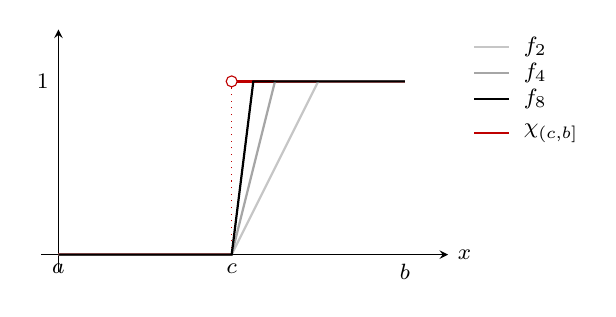
\begin{tikzpicture}[scale=2.2, >=stealth]
    \draw[->] (-0.1,0) -- (2.25,0) node[right] {$x$};
    \draw[->] (0,-0.1) -- (0,1.3);
    \node[below] at (0,0) {$a$};
    \node[below] at (1,0) {$c$};
    \node[below] at (2,0) {$b$};
    \node[left] at (0,1) {$1$};
    \draw[very thick, red!75!black] (0,0) -- (1,0);
    \draw[very thick, red!75!black] (1,1) -- (2,1);
    \draw[dotted, red!75!black] (1,0) -- (1,1);
    \draw[red!75!black, fill=white] (1,1) circle (0.9pt);
    \foreach \n/\st in {2/gray!45, 4/gray!70, 8/black}
        \draw[thick, \st] (0,0) -- (1,0) -- ({1+1/\n},1) -- (2,1);
    \foreach \y/\st/\lab in {1.2/gray!45/{$f_2$}, 1.05/gray!70/{$f_4$}, 0.9/black/{$f_8$}, 0.7/{red!75!black}/{$\chi_{(c,b]}$}} {
        \draw[thick, \st] (2.4,\y) -- (2.6,\y);
        \node[anchor=west] at (2.63,\y) {\lab};
    }
\end{tikzpicture}
\end{center}
The ramps of Step~2 for $n = 2, 4, 8$ on $[a,b]$, with $c$ the midpoint. They differ from one another only near $c$, so they are Cauchy in $L^p$; an $L^p$ limit would have to be $0$ on $[a,c]$ and $1$ on $(c,b]$ --- the step function, which is not continuous.

\begin{rembox}\label{rem:completion-L1-sec-2}
This is the example to keep in mind for what the abstract construction of the completion does in practice. Started from continuous functions --- concrete, classical objects --- and measured in the $L^p$ norm, the completion is forced to contain discontinuous and even badly behaved functions, and it is exactly $L^p$. The ramp functions of Step 2 converge in $L^p$ to the class of the step function $\chi_{(c,b]}$, and Step 2 is precisely the statement that this class contains no continuous representative. Read backwards, the proposition says that $L^p[a,b]$ \emph{could} have been \emph{defined} as the completion of $C[a,b]$ in the $L^p$ norm, with no measure theory at all; that is one standard route to the Lebesgue spaces, and it is the definition Lax adopts (\S5.1, example (f)), and it explains Wu's remark that ``when we write $L^1[a,b]$, intuitively we are taking this norm.''
\end{rembox}

% ============================================================================
% SECTION 15: COMPACTNESS AND THE UNIT BALL
% ============================================================================
% Lecture 6 (2026-09-17)

\section{Compactness and the Unit Ball}\label{sec:noncompact}

\roadmark{Stage: norms}{Thread: dimension. The first structural difference between finite and infinite dimension.}

The spaces of this chapter are the first infinite-dimensional normed spaces available, so they are the first place where infinite dimension can be seen to make a difference. Here is the most basic such difference. In $\mathbb{R}^n$ a bounded sequence has a convergent subsequence, and this one fact carries much of classical analysis: it is how maxima are shown to be attained, how solutions of equations are extracted from approximating sequences, how limits are produced when no formula for them is available. It fails in every infinite-dimensional normed space, and the failure is not marginal --- the closed unit ball, the most basic bounded set there is, is never compact.

\subsection{Sequential Compactness}

\begin{defbox}[Sequentially Compact]\boxlabel{def:sequentially-compact}
A subset $K$ of a normed linear space (or metric space) $X$ is \textbf{sequentially compact}, or here simply \textbf{compact}, if every sequence $\{x_n\} \subset K$ has a subsequence $\{x_{n_k}\}$ converging to some $x_0 \in K$.
\end{defbox}

\begin{exbox}[The Closed Unit Ball in $\mathbb{F}^n$]\boxlabel{ex:closed-unit-ball-fn}
In $\mathbb{F}^n$ ($\mathbb{F} = \mathbb{R}$ or $\mathbb{C}$) with any norm, the closed unit ball
\[
\overline{B_1(0)} = \{ x \in \mathbb{F}^n : \|x\| \le 1 \}
\]
is compact. Indeed a sequence in it is coordinatewise bounded, so the diagonal extraction used in Step 5 of Theorem~\ref{prop:norms-equiv} --- Bolzano--Weierstrass applied $n$ times --- produces a subsequence converging coordinatewise, hence in norm, and the limit still satisfies $\|x_0\| \le 1$ by continuity of the norm (Proposition~\ref{prop:norm-continuous}).
\end{exbox}

\begin{defbox}[Open Set; Open Cover; Compact]\boxlabel{def:compact}
Let $X$ be a normed linear space (or metric space). A subset $U \subset X$ is \textbf{open} if every point of $U$ is a metric interior point of $U$ (Definition~\ref{def:metric-interior}). An \textbf{open cover} of $K \subset X$ is a collection of open sets whose union contains $K$. $K$ is \textbf{compact} if every open cover of $K$ has a finite subcollection that still covers $K$.
\end{defbox}

\begin{thmbox}[Compactness in Metric Spaces]\boxlabel{thm:compact-seq}
A subset of a normed linear space (or metric space) is compact if and only if it is sequentially compact.
\end{thmbox}

\begin{proof}
Not covered in lecture: the question was raised in class and set aside. This is point-set topology; see J.~Munkres, \emph{Topology}, \S28.
\end{proof}

\begin{rembox}[Which Compactness]\label{rem:which-compactness}
Only the sequential form is used in these notes, and Theorem~\ref{thm:compact-seq} is not needed for anything that follows; it records that ``compact'' is unambiguous here.
\end{rembox}

\subsection{Riesz's Lemma}

Without an inner product there is no notion of perpendicularity, so one cannot ask for a unit vector orthogonal to a subspace. The following lemma is the substitute available in a bare normed space: a unit vector that is at least a fixed distance from the subspace.

\begin{lembox}[Riesz's Lemma]\boxlabel{lem:riesz}
Let $(X, \|\cdot\|)$ be a normed linear space and $Y$ a closed proper subspace of $X$. Then there exists $z \in X$ with
\[
\|z\| = 1 \qquad \text{and} \qquad \operatorname{dist}(z, Y) = \inf_{y \in Y} \|z - y\| \ge \tfrac{1}{2}.
\]
\laxref{\S5.2, Lemma~7}
\end{lembox}

\begin{proof}
\textbf{Step 1: a point off $Y$, at positive distance.} Since $Y \subsetneq X$, choose $x_0 \in X \setminus Y$ and set
\[
d = \operatorname{dist}(x_0, Y) = \inf_{y \in Y} \|x_0 - y\|.
\]
Then $d > 0$. For if $d = 0$, there are $y_n \in Y$ with $\|x_0 - y_n\| \to 0$, i.e.\ $y_n \to x_0$; since $Y$ is closed (Definition~\ref{def:closed}) this forces $x_0 \in Y$, contrary to the choice of $x_0$. This is the only place closedness of $Y$ is used, and it is essential.

\textbf{Step 2: an almost-minimizing $y_0$.} The infimum $d$ need not be attained, but $2d > d$ is not a lower bound for $\{\|x_0 - y\| : y \in Y\}$, so there is $y_0 \in Y$ with
\[
d \le a := \|x_0 - y_0\| < 2d.
\]
(Any factor $>1$ would do here; see Corollary~\ref{cor:riesz-theta}.) Note $a > 0$.

\textbf{Step 3: normalize.} Put
\[
z = \frac{x_0 - y_0}{\|x_0 - y_0\|} = \frac{x_0 - y_0}{a}, \qquad \text{so } \|z\| = 1
\]
by homogeneity. For any $y \in Y$,
\[
z - y = \frac{x_0 - y_0}{a} - y = \frac{1}{a}\bigl( x_0 - (y_0 + a y) \bigr),
\]
and $y_0 + a y \in Y$ because $Y$ is a subspace. Hence, by homogeneity and the definition of $d$ as an infimum over all of $Y$,
\[
\|z - y\| = \frac{1}{a}\,\bigl\| x_0 - (y_0 + a y) \bigr\| \ge \frac{d}{a}.
\]
Taking the infimum over $y \in Y$ and using $a < 2d$,
\[
\operatorname{dist}(z, Y) \ge \frac{d}{a} > \frac{d}{2d} = \frac{1}{2}. \qedhere
\]
\end{proof}

\begin{center}
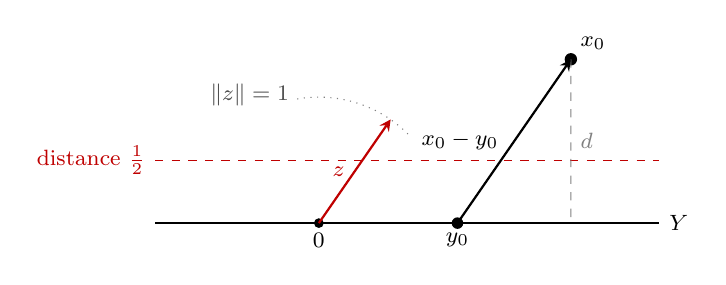
\begin{tikzpicture}[scale=1.6, >=stealth]
    \draw[thick] (-1.3,0) -- (2.7,0) node[right] {$Y$};
    \draw[dashed, red!75!black] (-1.3,0.5) -- (2.7,0.5);
    \node[left, red!75!black] at (-1.3,0.5) {distance $\tfrac12$};
    \fill (0,0) circle (1.1pt) node[below] {$0$};
    \coordinate (X0) at (2.0,1.3);
    \coordinate (Y0) at (1.1,0);
    \fill (X0) circle (1.4pt) node[above right] {$x_0$};
    \draw[dashed, gray] (X0) -- (2.0,0) node[midway, right] {$d$};
    \fill (Y0) circle (1.3pt) node[below] {$y_0$};
    \draw[->, thick] (Y0) -- (X0) node[midway, left, xshift=-2pt] {$x_0 - y_0$};
    \draw[dotted, gray] (45:1) arc (45:100:1);
    \draw[->, thick, red!75!black] (0,0) -- (0.570,0.823) node[midway, left, red!75!black] {$z$};
    \node[gray!60!black] at (-0.55,1.02) {$\|z\| = 1$};
\end{tikzpicture}
\end{center}
The picture drawn in Lecture~6, for $Y$ a line in $\mathbb{R}^2$: $y_0$ is only an almost-closest point, $d \le a = \|x_0 - y_0\| < 2d$, and $z = (x_0 - y_0)/a$ is the unit vector in the same direction. Every point of $Y$ is at distance at least $d/a > \tfrac12$ from $z$; here $z$ lies above the dashed line.

\begin{corbox}[Riesz's Lemma with Any Constant Below One]\boxlabel{cor:riesz-theta}
Under the hypotheses of Lemma~\ref{lem:riesz}, for every $\theta \in (0,1)$ there is $z \in X$ with $\|z\| = 1$ and $\operatorname{dist}(z, Y) \ge \theta$.
\end{corbox}

\begin{proof}
Repeat the proof of Lemma~\ref{lem:riesz}, choosing $y_0$ in Step 2 with $d \le a < d/\theta$, which is possible because $d/\theta > d$. Step 3 then gives $\operatorname{dist}(z, Y) \ge d/a > \theta$. (Not covered in lecture.)
\end{proof}

\begin{propbox}[{{The Constant $\theta = 1$ Cannot Be Attained}}]\boxlabel{prop:riesz-sharp}
Let $X = \{ f \in C[0,1] : f(0) = 0 \}$ with $\|f\| = \max_{[0,1]} |f|$, and
\[
Y = \Bigl\{ f \in X : \int_0^1 f(t)\,dt = 0 \Bigr\}.
\]
Then $X$ is a Banach space, $Y$ is a closed proper subspace of $X$, and
\[
\operatorname{dist}(f, Y) < 1 \qquad \text{for every } f \in X \text{ with } \|f\| = 1 .
\]
In particular Corollary~\ref{cor:riesz-theta} fails for $\theta = 1$.
\end{propbox}

\begin{proof}
Write $\varphi(h) = \int_0^1 h(t)\,dt$ for $h \in C[0,1]$. Then $\varphi$ is linear, and $|\varphi(h)| \le \int_0^1 |h| \le \|h\|$.

\textbf{Step 1: $X$ is a Banach space.} $X$ is a linear subspace of the Banach space $(C[0,1], \|\cdot\|_\infty)$ (Theorem~\ref{thm:Cab-banach}), and it is closed: if $f_n \in X$ and $f_n \to f$ uniformly, then $f(0) = \lim_n f_n(0) = 0$. A Cauchy sequence in $X$ is Cauchy in $C[0,1]$, so it converges there, and by closedness its limit lies in $X$. Hence $X$ is complete.

\textbf{Step 2: $Y$ is a closed proper subspace.} $Y$ is a subspace by linearity of $\varphi$. If $f_n \in Y$ and $f_n \to f \in X$, then $|\varphi(f)| = |\varphi(f - f_n)| \le \|f - f_n\| \to 0$, so $\varphi(f) = 0$ and $f \in Y$; thus $Y$ is closed. The function $g(t) = t$ lies in $X$ and has $\varphi(g) = \frac12 \neq 0$, so $Y \neq X$.

\textbf{Step 3: an upper bound for the distance.} For $n \ge 1$ let $g_n(t) = \min\{nt, 1\}$. Then $g_n \in X$, $\|g_n\| = 1$, and
\[
\varphi(g_n) = \int_0^{1/n} nt\,dt + \int_{1/n}^1 dt = \frac{1}{2n} + 1 - \frac{1}{n} = 1 - \frac{1}{2n} > 0 .
\]
Given $f \in X$, put
\[
y_n = f - \frac{\varphi(f)}{\varphi(g_n)}\, g_n .
\]
Then $y_n \in X$ and $\varphi(y_n) = \varphi(f) - \varphi(f) = 0$, so $y_n \in Y$. Hence
\[
\operatorname{dist}(f, Y) \le \|f - y_n\| = \frac{|\varphi(f)|}{\varphi(g_n)}\,\|g_n\| = \frac{|\varphi(f)|}{1 - \frac{1}{2n}} .
\]

\textbf{Step 4: $|\varphi(f)| < 1$ for unit vectors.} Let $f \in X$ with $\|f\| = 1$. Since $f$ is continuous and $f(0) = 0$, there is $\delta \in (0,1]$ with $|f(t)| \le \frac12$ for $0 \le t \le \delta$. Using $|f| \le 1$ on $[\delta, 1]$,
\[
|\varphi(f)| \le \int_0^\delta |f| + \int_\delta^1 |f| \le \frac{\delta}{2} + (1 - \delta) = 1 - \frac{\delta}{2} .
\]

\textbf{Step 5: conclusion.} Choose $n > 1/\delta$, so that $1 - \frac{1}{2n} > 1 - \frac{\delta}{2}$. By Steps 3 and 4,
\[
\operatorname{dist}(f, Y) \le \frac{1 - \delta/2}{1 - 1/(2n)} < 1 . \qedhere
\]
\end{proof}

\begin{rembox}[On the Constant]\label{rem:constant}
Since $0 \in Y$, always $\operatorname{dist}(z, Y) \le \|z - 0\| = 1$ for a unit vector $z$. So Corollary~\ref{cor:riesz-theta} says $\sup_{\|z\| = 1} \operatorname{dist}(z, Y) = 1$ for every closed proper subspace, and Proposition~\ref{prop:riesz-sharp} says the supremum need not be attained. The mechanism is visible in Steps 3--4: letting $n \to \infty$ in Step 3 gives $\operatorname{dist}(f, Y) \le |\int_0^1 f|$, so a unit vector at distance $1$ from $Y$ would need $|\int_0^1 f| = 1 = \max |f|$, which forces $|f| \equiv 1$ and is ruled out by $f(0) = 0$.

By contrast, in an inner product space the constant $1$ is attained as soon as a unit vector $z$ orthogonal to $Y$ is available (for a closed proper subspace of a Hilbert space, Theorem~\ref{thm:orth-decomp} provides one: take $x_0 \notin Y$ and normalize its $Y^\perp$-component): then $\|z - y\|^2 = \|z\|^2 - (z,y) - (y,z) + \|y\|^2 = 1 + \|y\|^2 \ge 1$ for every $y \in Y$. In general the picture Wu drew is the right one: $z$ is a unit vector pointing ``away from'' $Y$, and if a first attempt sits too close to $Y$ one slides along until it does not. (Not covered in lecture.)
\end{rembox}

\subsection{The Theorem}

\begin{thmbox}[The Unit Ball of an Infinite-Dimensional Space is Not Compact]\boxlabel{thm:ball-noncompact}
Let $X$ be an infinite-dimensional normed linear space. Then the closed unit ball
\[
\overline{B_1(0)} = \{ x \in X : \|x\| \le 1 \}
\]
is not compact.
\laxref{\S5.2, Thm~6}
\end{thmbox}

\begin{proof}
It suffices to construct a sequence $\{x_n\} \subset X$ with
\[
\|x_n\| = 1 \text{ for all } n, \qquad \|x_i - x_j\| \ge \tfrac{1}{2} \text{ for all } i \ne j.
\]
Such a sequence lies in $\overline{B_1(0)}$ and no subsequence of it is Cauchy --- the mutual distances never drop below $\tfrac12$ --- so no subsequence converges.

The construction is by induction, using Riesz's lemma at each step.

\emph{Base step.} Choose any $x_1 \in X$ with $\|x_1\| = 1$ (possible since $X \ne \{0\}$: take any nonzero vector and divide by its norm).

\emph{Induction step.} Suppose $x_1, \ldots, x_m$ have been constructed with $\|x_i\| = 1$ for $1 \le i \le m$ and $\operatorname{dist}(x_j, Y_{j-1}) \ge \tfrac12$ for $2 \le j \le m$, where $Y_{j-1} = \operatorname{span}\{x_1, \ldots, x_{j-1}\}$. Put
\[
Y_m = \operatorname{span}\{x_1, \ldots, x_m\}.
\]
Then:
\begin{itemize}
    \item $Y_m$ is \emph{closed}, because it is finite-dimensional (Corollary~\ref{cor:findim-closed});
    \item $Y_m$ is a \emph{proper} subspace of $X$, because $\dim Y_m \le m < \infty$ while $X$ is infinite-dimensional, so $X$ cannot equal the span of finitely many vectors.
\end{itemize}
Riesz's lemma (Lemma~\ref{lem:riesz}) applied to $Y_m \subsetneq X$ therefore produces $x_{m+1} \in X$ with $\|x_{m+1}\| = 1$ and $\operatorname{dist}(x_{m+1}, Y_m) \ge \tfrac12$.

\emph{Conclusion.} This produces $\{x_m\}_{m=1}^\infty \subset X$ with $\|x_m\| = 1$ for all $m$, and for $j < m$ we have $x_j \in Y_{m-1}$, hence
\[
\|x_m - x_j\| \ge \operatorname{dist}(x_m, Y_{m-1}) \ge \tfrac{1}{2}. \qedhere
\]
\end{proof}

\begin{rembox}[Where Infinite-Dimensionality Enters]\label{rem:where-infinite-dimensionality-enters}
This was asked in lecture. The hypothesis is used at exactly one point: to know that $Y_m = \operatorname{span}\{x_1, \ldots, x_m\}$ is a \emph{proper} subspace, so that Riesz's lemma applies and the construction can continue. In a finite-dimensional space the process halts --- at some stage $Y_m = X$, and there is no vector left at distance $\tfrac12$ from everything already chosen. Infinite-dimensionality is what guarantees a genuinely new direction at every step. The other hypothesis doing work is Corollary~\ref{cor:findim-closed}: without knowing $Y_m$ closed, Riesz's lemma would not apply either.
\end{rembox}

\begin{exbox}[The Separated Sequence in $\ell^p$]\boxlabel{ex:separated-sequence-l-p}
For $\ell^p$ with $1 \le p < \infty$ the construction can be written down without any induction. Let $e_j = (0, \ldots, 0, 1, 0, \ldots)$ with the $1$ in the $j$-th place. Then $\|e_j\|_p = 1$, and for $i \ne j$ the sequence $e_i - e_j$ has exactly two nonzero entries, $\pm 1$, so
\[
\|e_i - e_j\|_p = \bigl(1^p + 1^p\bigr)^{1/p} = 2^{1/p} > 1 > \tfrac12.
\]
Hence $\{e_j\}$ has no convergent subsequence, and the closed unit ball of $\ell^p$ is not compact. (In $\ell^\infty$, $\|e_i - e_j\|_\infty = 1$.) The theorem says that every infinite-dimensional normed space contains a sequence behaving like this one, even when no basis is available to write it down.
\end{exbox}

\begin{rembox}[Why This Matters: Toward Weak Convergence]\label{rem:why-this-matters-toward-weak-convergence}
Compactness is what allows a limit to be produced when no formula for it exists. The model application: to solve an equation $P(x) = 1$ one constructs approximate solutions, $P(x_1) \approx 1$, $P(x_2)$ closer, and so on, with $\|x_j\| \le M$ for all $j$; in finite dimensions the bounded sequence $\{x_j\}$ has a convergent subsequence, and its limit solves the equation provided $P$ is continuous. Theorem~\ref{thm:ball-noncompact} says this move is unavailable in the function spaces the course is about --- $L^p$, $\ell^p$, $C[a,b]$ are all infinite-dimensional.

The response is not to give up on compactness but to weaken the notion of convergence until it returns. A bounded sequence in a suitable infinite-dimensional space does have a subsequence converging \emph{weakly}, and the closed unit ball is compact in a weaker topology. This is the direction the course takes later; the present theorem is what makes it necessary.
\end{rembox}

% ============================================================================
% CHAPTER 5: INNER PRODUCT SPACES
% ============================================================================
% Lecture 6 (2026-09-17)

\chapter{Inner Product Spaces}

A norm measures length. An inner product measures length \emph{and} angle, and in particular gives a meaning to perpendicularity --- the structure whose absence forced the quotient space to stand in for the orthogonal complement in \S\ref{subsec:quotient} and forced Riesz's lemma to stand in for an orthogonal unit vector in \ref{sec:noncompact}. Spaces carrying one are much closer to $\mathbb{R}^n$ than a general normed space is, and are the setting for the strongest results of the subject.

\section{Definition and Examples}\label{sec:inner-def}

\roadmark{Stage: inner products}{Length and angle; $\ell^2$ and $L^2$.}

\begin{defbox}[Inner Product; Scalar Product]\boxlabel{def:inner-product}
Let $X$ be a linear space over $\mathbb{F}$ and let $(\cdot, \cdot) : X \times X \to \mathbb{F}$ be a function.

If $\mathbb{F} = \mathbb{R}$, it is an \textbf{inner product} (or \textbf{scalar product}) if for all $x, y, z \in X$ and $a, b \in \mathbb{R}$:
\begin{enumerate}[label=(\arabic*)]
    \item \textbf{bilinearity}: $(ax + by,\, z) = a(x,z) + b(y,z)$ and $(x,\, ay + bz) = a(x,y) + b(x,z)$;
    \item \textbf{symmetry}: $(x,y) = (y,x)$;
    \item \textbf{positivity}: $(x,x) \ge 0$, and $(x,x) = 0$ if and only if $x = 0$.
\end{enumerate}

If $\mathbb{F} = \mathbb{C}$, it is an inner product if for all $x, y, z \in X$ and $a, b \in \mathbb{C}$:
\begin{enumerate}[label=(\arabic*$'$)]
    \item \textbf{sesquilinearity}: $(ax + by,\, z) = a(x,z) + b(y,z)$ and $(x,\, ay + bz) = \bar{a}(x,y) + \bar{b}(x,z)$;
    \item \textbf{skew-symmetry} (conjugate symmetry): $(x,y) = \overline{(y,x)}$;
    \item \textbf{positivity}: $(x,x) \ge 0$, and $(x,x) = 0$ if and only if $x = 0$.
\end{enumerate}
The pair $(X, (\cdot,\cdot))$ is an \textbf{inner product space} or \textbf{scalar product space}.
\laxref{\S6.1, (i)--(iii)}
\end{defbox}

\begin{rembox}[Reading the Complex Axioms]\label{rem:reading-complex-axioms}
Three points.

First, the placement of the conjugate is a convention: here the inner product is linear in the \emph{first} argument and conjugate-linear in the second, which is the usual convention in mathematics. Physics texts put the conjugate on the first argument. Nothing depends on the choice, but formulas must be read consistently, and every computation below uses this one.

Second, sesquilinearity forces the conjugate in the second slot: if the product were linear in both slots then, taking $a = i$ and $y = z = x$, skew-symmetry would give $i(x,x) = (ix, x) = \overline{(x, ix)} = \overline{i(x,x)} = -i\,\overline{(x,x)}$, which fails for $(x,x) > 0$. ``Sesqui'' is Latin for one and a half: linear in one argument, conjugate-linear in the other.

Third, positivity is a statement about a real number even though $(\cdot,\cdot)$ is complex-valued: skew-symmetry applied with $y = x$ gives $(x,x) = \overline{(x,x)}$, so $(x,x) \in \mathbb{R}$ automatically, and the inequality $(x,x) \ge 0$ makes sense. The real case is the special case of the complex one in which all values are real and conjugation does nothing. (The second and third points were not made in lecture.)
\end{rembox}

\begin{exbox}[Euclidean Spaces]\boxlabel{ex:euclidean-spaces}
On $\mathbb{R}^n$, $(x,y) = \sum_{i=1}^n x_i y_i$ is an inner product --- the dot product. On $\mathbb{C}^n$,
\[
(x,y) = \sum_{i=1}^n x_i \overline{y_i},
\]
where the conjugate on the second factor is exactly what makes $(x,x) = \sum_i |x_i|^2 \ge 0$, and is the source of the sesquilinearity convention above.
\end{exbox}

\begin{exbox}[$\ell^2$]\boxlabel{ex:box}
On $\ell^2$, the sequences $a = (a_1, a_2, \ldots)$ with $\|a\|_2 = \bigl(\sum_j |a_j|^2\bigr)^{1/2} < \infty$, define
\[
(a, b) = \sum_{i=1}^{\infty} a_i \overline{b_i}.
\]
The series converges absolutely, by H\"older's inequality (Theorem~\ref{thm:holder-seq}) with $p = q = 2$:
\[
\sum_{i=1}^\infty \bigl| a_i \overline{b_i} \bigr| = \sum_{i=1}^\infty |a_i|\,|b_i| \le \|a\|_2\, \|b\|_2 < \infty .
\]
So the definition makes sense precisely on $\ell^2$, and nowhere else among the $\ell^p$: this is the one exponent for which the conjugate exponent is $p$ itself.
\laxref{\S6.1, Example~2}
\end{exbox}

\begin{exbox}[$L^2(\Omega)$]\boxlabel{ex:l2}
On $L^2(\Omega)$ define
\[
(f, g) = \int_\Omega f(x)\, \overline{g(x)}\, dx,
\]
the direct continuum analogue of the $\mathbb{C}^n$ dot product. The integral converges absolutely by H\"older for functions (Theorem~\ref{thm:holder-fn}) with $p = q = 2$: $\int_\Omega |f \bar g| \le \|f\|_{L^2}\|g\|_{L^2} < \infty$.
\end{exbox}

\begin{rembox}\label{rem:inner-def}
In each example $(x,x)$ is the square of the norm already attached to the space: $(x,x) = \|x\|_2^2$ on $\mathbb{R}^n$, $\ell^2$, and $L^2$. That is not a coincidence, and the next section shows it holds in general: every inner product determines a norm by $\|x\| = (x,x)^{1/2}$. Note the logical order --- an inner product space is a linear space with an inner product, no norm assumed; the norm is produced.
\end{rembox}

\section{Cauchy--Schwarz and the Induced Norm}\label{sec:cauchy-schwarz}

\roadmark{Stage: inner products}{Thread: convexity. Every inner product induces a norm, and the parallelogram law says which norms arise.}

\subsection{The Cauchy--Schwarz Inequality}

\begin{notebox}[Notation]\label{note:notation-5}
Throughout this section $(X, (\cdot,\cdot))$ is an inner product space and
\[
\|x\| := (x,x)^{1/2},
\]
which is well defined since $(x,x) \ge 0$. Calling it a norm is an abuse of language until Theorem~\ref{thm:inner-norm} below; Wu flagged this explicitly while writing the proof.
\end{notebox}

\begin{thmbox}[Cauchy--Schwarz]\boxlabel{thm:cauchy-schwarz}
For all $x, y$ in an inner product space $X$,
\[
|(x,y)| \le \|x\|\, \|y\|.
\]
\laxref{\S6.1, Thm~1}
\end{thmbox}

\begin{proof}
\textbf{Step 1: expand a square.} For $t \in \mathbb{F}$, positivity gives $(x + ty,\, x + ty) \ge 0$. Expanding by sesquilinearity,
\[
(x + ty,\, x + ty) = (x,x) + \bar{t}\,(x,y) + t\,(y,x) + t\bar{t}\,(y,y).
\]
By skew-symmetry $(x,y) = \overline{(y,x)}$, so $\bar t (x,y) = \overline{t (y,x)}$ and the two middle terms are a number plus its conjugate:
\begin{equation}\label{eq:cs-expand}
\|x + ty\|^2 = \|x\|^2 + 2\operatorname{Re}\bigl( t\,(y,x) \bigr) + |t|^2 \|y\|^2 \ \ge\ 0 \qquad \text{for all } t \in \mathbb{F}.
\end{equation}

\textbf{Step 2: restrict to real $t$ and read off a quadratic.} The inequality holds in particular for $t \in \mathbb{R}$, where $\operatorname{Re}(t(y,x)) = t \operatorname{Re}(y,x)$. Writing
\[
A = \|y\|^2, \qquad B = \operatorname{Re}(y,x), \qquad C = \|x\|^2,
\]
\eqref{eq:cs-expand} says
\[
A t^2 + 2Bt + C \ge 0 \qquad \text{for all } t \in \mathbb{R}.
\]

\textbf{Step 3: complete the square.} If $y = 0$ then both sides of the theorem are $0$ and there is nothing to prove, so assume $y \ne 0$; then $A = \|y\|^2 > 0$ by positivity. For $t \in \mathbb{R}$,
\[
A t^2 + 2Bt + C = A\Bigl( t + \frac{B}{A} \Bigr)^2 + C - \frac{B^2}{A} \ \ge\ 0 .
\]
Choosing $t = -B/A$ kills the square and leaves $C - B^2/A \ge 0$, i.e.
\[
B^2 \le AC, \qquad \text{that is} \qquad \bigl| \operatorname{Re}(y,x) \bigr| \le \|x\|\,\|y\|.
\]

\textbf{Step 4: remove the real part by rotating.} Over $\mathbb{R}$ this already is the theorem. Over $\mathbb{C}$, write the complex number $(y,x)$ in polar form and choose $\theta$ with
\[
|(y,x)| = e^{i\theta}\,(y,x).
\]
By linearity in the first argument, $e^{i\theta}(y,x) = (e^{i\theta} y,\, x)$. So $(e^{i\theta}y, x)$ is a non-negative real number, hence equal to its own real part, and Step 3 applied to the pair $e^{i\theta}y$, $x$ gives
\[
|(y,x)| = \operatorname{Re}\bigl( e^{i\theta} y,\, x \bigr) \le \bigl\| e^{i\theta} y \bigr\|\, \|x\| = \|y\|\,\|x\|,
\]
where the last equality is
\[
\bigl\| e^{i\theta} y \bigr\|^2 = \bigl( e^{i\theta} y,\, e^{i\theta} y \bigr) = e^{i\theta}\,\overline{e^{i\theta}}\,(y,y) = |e^{i\theta}|^2 \|y\|^2 = \|y\|^2 .
\]
Finally $|(x,y)| = |\overline{(y,x)}| = |(y,x)|$, so the bound holds in the stated order as well.
\end{proof}

\subsection{The Induced Norm and Hilbert Spaces}

\begin{thmbox}[The Inner Product Induces a Norm]\boxlabel{thm:inner-norm}
Let $(X, (\cdot,\cdot))$ be an inner product space. Then $\|x\| = (x,x)^{1/2}$ is a norm on $X$, so $(X, \|\cdot\|)$ is a normed linear space.
\laxref{\S6.1, (3)}
\end{thmbox}

\begin{proof}
\emph{Positivity} is axiom (3): $\|x\| = (x,x)^{1/2} \ge 0$, and $\|x\| = 0$ iff $(x,x) = 0$ iff $x = 0$.

\emph{Homogeneity.} By sesquilinearity, for $a \in \mathbb{F}$,
\[
\|ax\|^2 = (ax, ax) = a \bar{a}\, (x,x) = |a|^2 \|x\|^2,
\]
and taking non-negative square roots gives $\|ax\| = |a|\,\|x\|$.

\emph{Subadditivity.} This is the only part needing Cauchy--Schwarz. Expanding as in \eqref{eq:cs-expand} with $t = 1$ and $y$ in place of $ty$,
\[
\|x + y\|^2 = \|x\|^2 + 2\operatorname{Re}(x,y) + \|y\|^2 \le \|x\|^2 + 2\,|(x,y)| + \|y\|^2 \le \|x\|^2 + 2\|x\|\,\|y\| + \|y\|^2,
\]
using $\operatorname{Re} w \le |w|$ and then Theorem~\ref{thm:cauchy-schwarz}. The right-hand side is $\bigl( \|x\| + \|y\| \bigr)^2$, so taking square roots gives $\|x + y\| \le \|x\| + \|y\|$.
\end{proof}

\begin{rembox}\label{rem:cauchy-schwarz}
So every inner product space is a normed linear space, and all of Chapters 3 and 4 applies to it. The converse question --- which norms come from an inner product --- is answered in \S\ref{subsec:parallelogram}.
\end{rembox}

\begin{defbox}[Hilbert Space]\boxlabel{def:hilbert}
An inner product space that is complete in the induced norm $\|x\| = (x,x)^{1/2}$ is a \textbf{Hilbert space}.
\laxref{\S6.1, definition of Hilbert space}
\end{defbox}

\begin{exbox}[Hilbert Spaces]\boxlabel{ex:hilbert-spaces}
$\mathbb{R}^n$ and $\mathbb{C}^n$ with the dot product are Hilbert spaces, being finite-dimensional (Corollary~\ref{cor:findim-complete}); so are $\ell^2$ and $L^2(\Omega)$ with the inner products of \ref{sec:inner-def}, complete by Theorems~\ref{thm:lp-complete} and~\ref{thm:Lp-complete}. Wu: ``I proved all $L^p$ is complete; I should at some point put my proof online.''
\end{exbox}

% Lecture 7 (2026-09-22)
\begin{exbox}[An Inner Product Space that is Not a Hilbert Space]\boxlabel{ex:an-inner-product-space}
Let $X = C_c(\mathbb{R}^n)$, the continuous functions with compact support (the set where $f \neq 0$ is contained in a bounded set, so $f$ is integrable), with
\[
(f, g) = \int_{\mathbb{R}^n} f(x)\,\overline{g(x)}\,dx .
\]
This is the inner product of $L^2(\mathbb{R}^n)$ restricted to $X$, so $(X, (\cdot,\cdot))$ is an inner product space. It is not complete: $C_c(\mathbb{R}^n)$ is dense in $L^2(\mathbb{R}^n)$ (Theorem~\ref{thm:density}), so any $F \in L^2 \setminus C_c$ is the $L^2$-limit of a sequence in $X$, which is then Cauchy in $X$ with no limit in $X$. By Proposition~\ref{prop:identify-completion}, $\overline{X} = L^2(\mathbb{R}^n)$. (The same argument, with the same conclusion, applies to $C_c^\infty$.)
\laxref{\S6.1, Example~1}
\end{exbox}

\begin{exbox}[Sobolev Spaces]\boxlabel{ex:sobolev}
Let $\Omega \subset \mathbb{R}^n$ be a domain, $k \ge 0$ an integer, and $X = C_c^\infty(\Omega)$, the smooth functions whose support is a compact subset of $\Omega$. For a multi-index $\alpha = (\alpha_1, \ldots, \alpha_n)$ write $|\alpha| = \alpha_1 + \cdots + \alpha_n$ and
\[
\partial^\alpha f = \partial_{x_1}^{\alpha_1} \partial_{x_2}^{\alpha_2} \cdots \partial_{x_n}^{\alpha_n} f ,
\]
which makes sense for every $\alpha$ because $f$ is $C^\infty$, and is again in $C_c^\infty(\Omega)$. Define
\[
(f, g) = \sum_{|\alpha| \le k} \int_\Omega \partial^\alpha f(x)\, \overline{\partial^\alpha g(x)}\,dx .
\]
Each summand is the $L^2$ inner product of two functions in $C_c^\infty$, so this is an inner product on $X$ (a finite sum of inner products with the same sesquilinearity and symmetry; positivity from the $\alpha = 0$ term). The induced norm is $\|f\|^2 = \sum_{|\alpha| \le k} \|\partial^\alpha f\|_{L^2}^2$, which controls $f$ and all its derivatives up to order $k$ in $L^2$. For $k = 0$ this is the previous example. $X$ is not complete; its completion is a \textbf{Sobolev space}, denoted $H^k_0(\Omega)$, the subscript recording that it comes from functions with compact support in $\Omega$. Lax (\S5.1, example (g)) instead completes the $C^\infty$ functions on $\Omega$ for which the norm is finite, with no support condition, and calls the result $W^{k,p}$; for $p = 2$ it is written $H^k(\Omega)$. Informally, elements of either completion are functions whose derivatives up to order $k$ lie in $L^2$; making this precise requires weak derivatives, which the course does not develop.

Wu's motivation: if $f$ is a velocity, $\int |f|^2$ is an energy, and a physical process with finite, conserved energy naturally lives in a space of this type; the completion is what makes limits of approximate solutions available. This is the setting of the modern theory of partial differential equations, but the course stays with functional analysis.
\laxref{\S5.1, example (g)}
\end{exbox}

\subsection{Which Norms Come from an Inner Product}\label{subsec:parallelogram}

\begin{propbox}[Parallelogram Law and Polarization]\boxlabel{prop:parallelogram}
Let $(X, (\cdot,\cdot))$ be an inner product space and $\|x\| = (x,x)^{1/2}$. For all $x, y \in X$:
\begin{enumerate}[label=(\alph*)]
    \item (parallelogram law) $\|x + y\|^2 + \|x - y\|^2 = 2\|x\|^2 + 2\|y\|^2$;
    \item (polarization) if $\mathbb{F} = \mathbb{R}$, $(x,y) = \frac14\bigl( \|x+y\|^2 - \|x-y\|^2 \bigr)$; if $\mathbb{F} = \mathbb{C}$,
    \[
    (x,y) = \frac14 \bigl( \|x+y\|^2 - \|x-y\|^2 \bigr) + \frac{i}{4} \bigl( \|x+iy\|^2 - \|x-iy\|^2 \bigr) = \frac14 \sum_{k=0}^{3} i^k\, \|x + i^k y\|^2 .
    \]
\end{enumerate}
In particular an inner product is determined by the norm it induces.
\laxref{\S6.1, (6)}
\end{propbox}

\begin{proof}
(Part (b) not covered in lecture.) By \eqref{eq:cs-expand} with $t = \pm 1$, and since $(x,y)$ and $(y,x)$ are conjugate and so have the same real part,
\[
\|x \pm y\|^2 = \|x\|^2 \pm 2\operatorname{Re}(x,y) + \|y\|^2 .
\]
Adding the two gives (a): in Wu's words, ``$t$ positive cancels with $t$ negative.'' Subtracting gives $\|x+y\|^2 - \|x-y\|^2 = 4\operatorname{Re}(x,y)$, which is (b) when $\mathbb{F} = \mathbb{R}$. When $\mathbb{F} = \mathbb{C}$, apply the same identity to $x$ and $iy$: since $(x, iy) = \bar{i}\,(x,y) = -i(x,y)$,
\[
\|x+iy\|^2 - \|x-iy\|^2 = 4\operatorname{Re}\bigl( -i(x,y) \bigr) = 4\operatorname{Im}(x,y),
\]
and $(x,y) = \operatorname{Re}(x,y) + i\operatorname{Im}(x,y)$ is the formula in (b).
\end{proof}

The parallelogram law is a statement of plane geometry: in the parallelogram spanned by $x$ and $y$, the diagonals are $x + y$ and $x - y$, and the squares of the two diagonals sum to the squares of the four sides.

\begin{center}
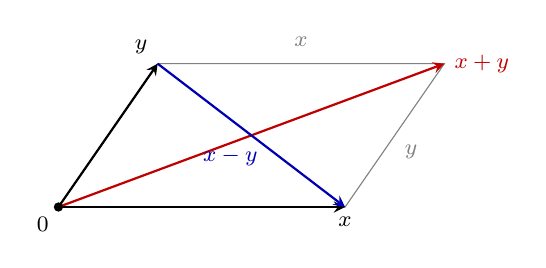
\begin{tikzpicture}[scale=1.4, >=stealth]
    \coordinate (O) at (0,0);
    \coordinate (X) at (2.6,0);
    \coordinate (Y) at (0.9,1.3);
    \coordinate (XY) at (3.5,1.3);
    \draw[thin, gray] (O) -- (X) -- (XY) -- (Y) -- cycle;
    \draw[->, thick] (O) -- (X) node[below, font=\footnotesize] {$x$};
    \draw[->, thick] (O) -- (Y) node[above left, font=\footnotesize] {$y$};
    \draw[->, thick, red!75!black] (O) -- (XY) node[right, font=\footnotesize] {$x + y$};
    \draw[->, thick, blue!70!black] (Y) -- (X) node[midway, below left, font=\footnotesize, xshift=6pt, yshift=-1pt] {$x - y$};
    \node[font=\footnotesize, gray] at (3.2,0.5) {$y$};
    \node[font=\footnotesize, gray] at (2.2,1.5) {$x$};
    \fill (O) circle (1.2pt) node[below left, font=\footnotesize] {$0$};
\end{tikzpicture}
\end{center}

The next theorem says it is the \emph{only} obstruction.

\begin{thmbox}[Jordan--von Neumann]\boxlabel{thm:jvn}
Let $(X, \|\cdot\|)$ be a normed linear space. There is an inner product $(\cdot,\cdot)$ on $X$ with $(x,x) = \|x\|^2$ for all $x \in X$ if and only if $\|\cdot\|$ satisfies the parallelogram law. The inner product is then unique, given by the polarization formula of Proposition~\ref{prop:parallelogram}(b).
\laxref{\S6.1, Exercise~1}
\end{thmbox}

\begin{proof}
Necessity and uniqueness are Proposition~\ref{prop:parallelogram}. (HW3, Problem 3.) 
For sufficiency, assume the parallelogram law
\[\|x + y\|^2 + \|x - y\|^2 = 2\bigl( \|x\|^2 + \|y\|^2 \bigr) \qquad \text{for all } x, y \in X. \tag{P}\]
We treat $\mathbb{F} = \mathbb{R}$ first and then reduce $\mathbb{F} = \mathbb{C}$ to it. Two properties of the norm are used repeatedly: $\|\lambda w\| = |\lambda|\,\|w\|$, in particular $\|{-w}\| = \|w\|$; and the norm is continuous, since $\bigl|\,\|u\| - \|v\|\,\bigr| \leq \|u - v\|$.

\textbf{Part 1: the real case.} Let $\mathbb{F} = \mathbb{R}$ and define
\[(x, y) := \frac14 \bigl( \|x + y\|^2 - \|x - y\|^2 \bigr), \qquad x, y \in X.\]

\emph{Step 1: symmetry and positivity.} Since $y + x = x + y$ and $\|y - x\| = \|{-(x - y)}\| = \|x - y\|$, we have $(y, x) = (x, y)$. Also
\[(x, x) = \frac14 \bigl( \|2x\|^2 - \|0\|^2 \bigr) = \frac14 \cdot 4\|x\|^2 = \|x\|^2,\]
so $(x,x) \geq 0$, with $(x,x) = 0$ if and only if $x = 0$, and $\|x\|^2 = (x,x)$.

\emph{Step 2: a midpoint identity.} We claim that
\[(x, z) + (y, z) = 2\Bigl( \frac{x + y}{2},\, z \Bigr) \qquad \text{for all } x, y, z \in X. \tag{1}\]
Put $u = \frac{x + y}{2}$ and $v = \frac{x - y}{2}$, so that $u + v = x$ and $u - v = y$. Applying (P) to the pair $u + z$, $v$ and to the pair $u - z$, $v$,
\begin{align*}
\|x + z\|^2 + \|y + z\|^2 &= \|(u + z) + v\|^2 + \|(u + z) - v\|^2 = 2\|u + z\|^2 + 2\|v\|^2, \\
\|x - z\|^2 + \|y - z\|^2 &= \|(u - z) + v\|^2 + \|(u - z) - v\|^2 = 2\|u - z\|^2 + 2\|v\|^2.
\end{align*}
Subtracting the second line from the first,
\[\bigl( \|x + z\|^2 - \|x - z\|^2 \bigr) + \bigl( \|y + z\|^2 - \|y - z\|^2 \bigr) = 2\bigl( \|u + z\|^2 - \|u - z\|^2 \bigr),\]
that is, $4(x,z) + 4(y,z) = 8(u,z)$, which is (1).

\emph{Step 3: additivity in the first argument.} First, $(0, z) = \frac14 \bigl( \|z\|^2 - \|{-z}\|^2 \bigr) = 0$. Taking $y = 0$ in (1) gives $(x, z) = 2\bigl( \frac{x}{2}, z \bigr)$ for every $x \in X$. Applying this with $x + y$ in place of $x$, and then (1),
\[(x + y, z) = 2\Bigl( \frac{x + y}{2}, z \Bigr) = (x, z) + (y, z).\]

\emph{Step 4: rational homogeneity.} We show $(ax, z) = a(x, z)$ for all $a \in \mathbb{Q}$. For $n \in \mathbb{N}$, induction on $n$ using Step 3 gives $(nx, z) = n(x, z)$, the case $n = 0$ being $(0, z) = 0$. Next,
\[(-x, z) = \frac14 \bigl( \|{-x} + z\|^2 - \|{-x} - z\|^2 \bigr) = \frac14 \bigl( \|x - z\|^2 - \|x + z\|^2 \bigr) = -(x, z),\]
so $(-nx, z) = -(nx, z) = -n(x, z)$, and the claim holds for all $a \in \mathbb{Z}$. Finally, for $m \in \mathbb{Z}$ and $n \in \mathbb{N}$ with $n \geq 1$,
\[n\Bigl( \frac{m}{n}x,\, z \Bigr) = \Bigl( n \cdot \frac{m}{n}x,\, z \Bigr) = (mx, z) = m(x, z),\]
and dividing by $n$ gives $\bigl( \frac{m}{n}x, z \bigr) = \frac{m}{n}(x, z)$.

\emph{Step 5: real homogeneity.} Fix $x, z \in X$ and define $\phi, \psi : \mathbb{R} \to \mathbb{R}$ by
\[\phi(a) = (ax, z) = \frac14 \bigl( \|ax + z\|^2 - \|ax - z\|^2 \bigr), \qquad \psi(a) = a\,(x, z).\]
The maps $a \mapsto ax \pm z$ are continuous from $\mathbb{R}$ to $X$, since $\|(ax \pm z) - (a'x \pm z)\| = |a - a'|\,\|x\|$; the norm is continuous; and $t \mapsto t^2$ is continuous. So $\phi$ is continuous, and so is $\psi$. By Step 4, $\phi = \psi$ on $\mathbb{Q}$. Given $a \in \mathbb{R}$, choose rationals $a_k \to a$; then
\[\phi(a) = \lim_{k} \phi(a_k) = \lim_{k} \psi(a_k) = \psi(a).\]
Hence $(ax, z) = a(x, z)$ for all $a \in \mathbb{R}$.

\emph{Step 6: conclusion.} By Steps 3 and 5, $(ax + by, z) = (ax, z) + (by, z) = a(x, z) + b(y, z)$ for all $a, b \in \mathbb{R}$, and by the symmetry of Step 1 the same holds in the second argument. Together with Step 1, $(\cdot,\cdot)$ is bilinear, symmetric and positive, i.e.\ a scalar product on $X$, and $(x, x) = \|x\|^2$ for all $x \in X$.

\textbf{Part 2: the complex case.} Let $\mathbb{F} = \mathbb{C}$ and define
\[(x, y) := \frac14 \bigl( \|x + y\|^2 - \|x - y\|^2 \bigr) + \frac{i}{4} \bigl( \|x + iy\|^2 - \|x - iy\|^2 \bigr), \qquad x, y \in X.\]
Writing $R(x, y) := \frac14 \bigl( \|x + y\|^2 - \|x - y\|^2 \bigr) \in \mathbb{R}$, this reads
\[(x, y) = R(x, y) + i\,R(x, iy). \tag{2}\]

\emph{Step 1: $R$ is a real scalar product.} Restricting scalar multiplication to $\mathbb{R}$ makes $X$ a linear space over $\mathbb{R}$; $\|\cdot\|$ is still a norm on it, and (P) still holds. By Part 1, $R$ is real-bilinear and symmetric, with $R(x, x) = \|x\|^2$.

\emph{Step 2: two identities.} For all $x, y \in X$,
\[\text{(i)}\ \ R(ix, iy) = R(x, y), \qquad \text{(ii)}\ \ R(ix, y) = -R(x, iy).\]
For (i): $\|ix \pm iy\| = \|i(x \pm y)\| = |i|\,\|x \pm y\| = \|x \pm y\|$. For (ii): since $i \cdot (-iy) = y$, identity (i) gives $R(ix, y) = R\bigl( ix, i(-iy) \bigr) = R(x, -iy)$, and $R(x, -iy) = -R(x, iy)$ by the real linearity of $R$ in its second argument.

\emph{Step 3: complex linearity in the first argument.} Additivity and real homogeneity, $(x + x', y) = (x, y) + (x', y)$ and $(ax, y) = a(x, y)$ for $a \in \mathbb{R}$, follow from (2) and the real bilinearity of $R$. For multiplication by $i$, by (2), (ii) and (i),
\[(ix, y) = R(ix, y) + i\,R(ix, iy) = -R(x, iy) + i\,R(x, y) = i\bigl( R(x, y) + i\,R(x, iy) \bigr) = i\,(x, y).\]
Hence, for $c = c_1 + ic_2$ with $c_1, c_2 \in \mathbb{R}$,
\[(cx, y) = \bigl( c_1 x + c_2\,(ix),\, y \bigr) = c_1 (x, y) + c_2 (ix, y) = c_1 (x, y) + i c_2 (x, y) = c\,(x, y),\]
and together with additivity, $(ax + by, z) = a(x, z) + b(y, z)$ for all $a, b \in \mathbb{C}$.

\emph{Step 4: skew-symmetry.} Since $R$ is real-valued, $\overline{(x, y)} = R(x, y) - i\,R(x, iy)$. On the other hand, by (2), the symmetry of $R$, and (ii),
\[(y, x) = R(y, x) + i\,R(y, ix) = R(x, y) + i\,R(ix, y) = R(x, y) - i\,R(x, iy).\]
So $(x, y) = \overline{(y, x)}$.

\emph{Step 5: conjugate linearity in the second argument.} By Steps 4 and 3,
\[(x, ay + bz) = \overline{(ay + bz, x)} = \overline{a(y, x) + b(z, x)} = \bar{a}\,\overline{(y, x)} + \bar{b}\,\overline{(z, x)} = \bar{a}\,(x, y) + \bar{b}\,(x, z).\]

\emph{Step 6: positivity.} By (2), $(x, x) = R(x, x) + i\,R(x, ix)$, where $R(x, x) = \|x\|^2$ and
\[R(x, ix) = \frac14 \bigl( \|(1 + i)x\|^2 - \|(1 - i)x\|^2 \bigr) = \frac14 \bigl( |1 + i|^2 - |1 - i|^2 \bigr) \|x\|^2 = 0.\]
Hence $(x, x) = \|x\|^2 \geq 0$, with equality if and only if $x = 0$.

By Steps 3--6, $(\cdot,\cdot)$ is sesquilinear, skew-symmetric and positive, i.e.\ a scalar product on $X$, and $(x, x) = \|x\|^2$ for all $x \in X$.
\end{proof}

\begin{rembox}\label{rem:cauchy-schwarz-2}
Two points about the proof. First, the only genuinely analytic step is real homogeneity: additivity yields it for rational scalars by pure algebra, and continuity of the norm extends it to the reals. Additivity alone would not suffice --- there exist additive functions $\mathbb{R} \to \mathbb{R}$ that are not linear, constructed from a Hamel basis --- which is why continuity must be invoked. Second, the complex case is reduced to the real one exactly as in the complex Hahn--Banach theorem: the real part determines everything, because $\operatorname{Im}(x,y) = \operatorname{Re}(x, iy)$, just as $\operatorname{Im}\ell(x) = -\operatorname{Re}\ell(ix)$ there.
\end{rembox}

\begin{corbox}[{{Only $p = 2$ Gives an Inner Product}}]\boxlabel{cor:only-p2}
Let $1 \le p \le \infty$ with $p \neq 2$. The norm $\|\cdot\|_p$ on $\mathbb{F}^n$ ($n \ge 2$), on $\ell^p$, and on $L^p(\Omega)$ does not come from an inner product.
\end{corbox}

\begin{proof}
By Theorem~\ref{thm:jvn} it suffices to exhibit $x, y$ violating the parallelogram law. In $\mathbb{F}^n$ and $\ell^p$ take $x = e_1$, $y = e_2$. In $L^p(\Omega)$ take disjoint $A, B \subset \Omega$ of positive measure (two disjoint small balls) and $x = \chi_A / m(A)^{1/p}$, $y = \chi_B / m(B)^{1/p}$, or $x = \chi_A$, $y = \chi_B$ if $p = \infty$. In each case $\|x\|_p = \|y\|_p = 1$ and $x, y$ have disjoint supports, so $|x \pm y|^p = |x|^p + |y|^p$ pointwise and $\|x \pm y\|_p = 2^{1/p}$ for $p < \infty$, while $\|x \pm y\|_\infty = 1$. The parallelogram law would require $\|x+y\|_p^2 + \|x-y\|_p^2 = 2 \cdot 2^{2/p}$ to equal $2(\|x\|_p^2 + \|y\|_p^2) = 4$, i.e.\ $2^{2/p} = 2$, i.e.\ $p = 2$; for $p = \infty$ it would require $2 = 4$. (Not covered in lecture.)
\end{proof}

% ============================================================================
% SECTION 18: PROJECTION AND ORTHOGONAL DECOMPOSITION
% ============================================================================
% Lecture 7 (2026-09-22)

\section{Projection and Orthogonal Decomposition}\label{sec:projection}

\roadmark{Stage: inner products}{Threads meet: convexity $\times$ completeness. Closest points; the orthogonal complement replaces the quotient of \S\ref{subsec:quotient}.}

Everything from here on uses completeness, and the results are the ones for which Hilbert spaces are named. Wu's comment on the method: much of what is proved below is familiar from $\mathbb{R}^n$, and the proofs there never used finite-dimensionality --- so they go through unchanged. The one new ingredient is that a closest point must be \emph{produced} as a limit, which is where completeness enters.

\subsection{Continuity of the Inner Product}

\begin{lembox}[The Inner Product is Continuous]\boxlabel{lem:ip-continuous}
Let $(X, (\cdot,\cdot))$ be an inner product space. If $x_n \to x_0$ and $y_n \to y_0$ in $X$, then $(x_n, y_n) \to (x_0, y_0)$ in $\mathbb{F}$.
\laxref{\S6.1, Exercise~2}
\end{lembox}

\begin{proof}
Insert $(x_0, y_n)$ and use sesquilinearity in each slot:
\[
(x_n, y_n) - (x_0, y_0) = (x_n - x_0,\, y_n) + (x_0,\, y_n - y_0).
\]
By the triangle inequality in $\mathbb{F}$ and Cauchy--Schwarz (Theorem~\ref{thm:cauchy-schwarz}),
\[
\bigl| (x_n, y_n) - (x_0, y_0) \bigr| \le \|x_n - x_0\|\,\|y_n\| + \|x_0\|\,\|y_n - y_0\| .
\]
The second term tends to $0$ because $\|y_n - y_0\| \to 0$ and $\|x_0\|$ is a fixed number. For the first term, $\|x_n - x_0\| \to 0$, and the factor $\|y_n\|$ is bounded: $\|y_n\| \le \|y_n - y_0\| + \|y_0\| \le M$ for some $M$, since a sequence tending to $0$ is bounded. So the first term is at most $M\|x_n - x_0\| \to 0$.
\end{proof}

\begin{rembox}\label{rem:projection}
The point Wu made in class: the factor $\|y_n\|$ cannot be dropped and cannot a priori be assumed bounded; that it is bounded follows from convergence of $y_n$, by subadditivity. Continuity in each variable separately ($x_n \to x_0$ with $y$ fixed) is the special case $y_n = y_0$, and is what is used below. Continuity of the norm (Proposition~\ref{prop:norm-continuous}) is the case $y_n = x_n$, $y_0 = x_0$.
\end{rembox}

\subsection{The Projection Theorem}

\begin{thmbox}[Closest Point in a Closed Convex Set]\boxlabel{thm:projection}
Let $H$ be a Hilbert space and $K \subset H$ a nonempty closed convex subset. For every $x_0 \in H$ there is a unique $y_0 \in K$ such that
\[
\|x_0 - y_0\| = \operatorname{dist}(x_0, K) := \inf_{y \in K} \|x_0 - y\| .
\]
\laxref{\S6.2, Thm~2}
\end{thmbox}

\begin{center}
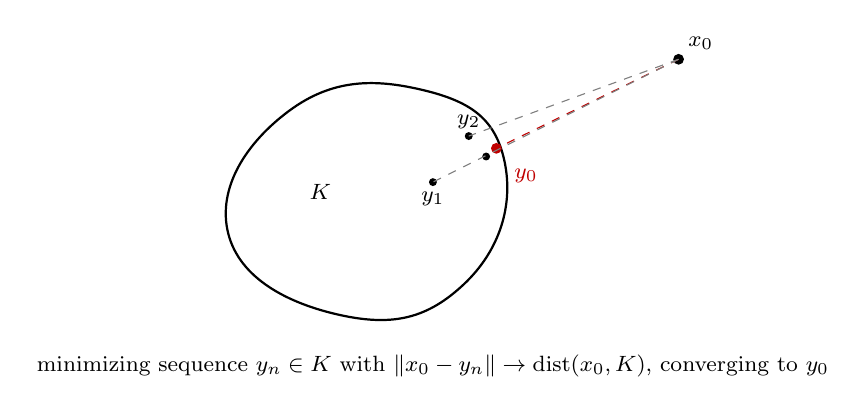
\begin{tikzpicture}[scale=1.3, >=stealth]
    \draw[thick] plot[smooth cycle, tension=0.8] coordinates {(-1.4,-0.3) (-0.8,0.9) (0.5,1.1) (1.3,0.4) (0.9,-0.8) (-0.3,-1.1)};
    \node[font=\footnotesize] at (-0.5,0.1) {$K$};
    \fill (3.0,1.4) circle (1.5pt) node[above right, font=\footnotesize] {$x_0$};
    \fill[red!75!black] (1.22,0.53) circle (1.5pt) node[below right, font=\footnotesize, xshift=3pt, yshift=-4pt] {$y_0$};
    \draw[dashed, red!75!black] (3.0,1.4) -- (1.22,0.53);
    \fill (0.6,0.2) circle (1.1pt) node[below, font=\footnotesize] {$y_1$};
    \fill (0.95,0.65) circle (1.1pt) node[above, font=\footnotesize, yshift=-1pt] {$y_2$};
    \fill (1.12,0.45) circle (1.1pt);
    \draw[dashed, gray] (3.0,1.4) -- (0.6,0.2);
    \draw[dashed, gray] (3.0,1.4) -- (0.95,0.65);
    \node[font=\footnotesize] at (0.6,-1.6) {minimizing sequence $y_n \in K$ with $\|x_0 - y_n\| \to \operatorname{dist}(x_0, K)$, converging to $y_0$};
\end{tikzpicture}
\end{center}

\begin{proof}
If $x_0 \in K$, take $y_0 = x_0$; it is unique since $\|x_0 - y\| = 0$ forces $y = x_0$. So assume $x_0 \notin K$ and put $d = \operatorname{dist}(x_0, K)$.

\textbf{Step 1: $d > 0$.} If $d = 0$ there would be $y_n \in K$ with $\|x_0 - y_n\| \to 0$, i.e.\ $y_n \to x_0$, and closedness of $K$ would give $x_0 \in K$.

\textbf{Step 2: a minimizing sequence.} Since $d$ is the greatest lower bound of $\{\|x_0 - y\| : y \in K\}$, for each $m \in \mathbb{N}$ there is $y_m \in K$ with
\begin{equation}\label{eq:minseq}
d^2 \le \|x_0 - y_m\|^2 < d^2 + \frac{1}{m}.
\end{equation}
(The first inequality holds for every point of $K$.) We show $\{y_m\}$ is Cauchy; it then converges by completeness of $H$, and its limit lies in $K$ by closedness.

\textbf{Step 3: Cauchy, via the parallelogram law.} Fix $m, n$. Apply the parallelogram law (Proposition~\ref{prop:parallelogram}(a)) to $a = x_0 - y_m$ and $b = x_0 - y_n$, so that $a + b = 2x_0 - (y_m + y_n)$ and $a - b = y_n - y_m$:
\[
\|2x_0 - (y_m + y_n)\|^2 + \|y_n - y_m\|^2 = 2\|x_0 - y_m\|^2 + 2\|x_0 - y_n\|^2 .
\]
The first term is $4\,\bigl\| x_0 - \tfrac{y_m + y_n}{2} \bigr\|^2$, and the midpoint $\tfrac{y_m + y_n}{2}$ lies in $K$ by convexity, so this term is at least $4d^2$. Rearranging and using \eqref{eq:minseq},
\[
\|y_n - y_m\|^2 = 2\|x_0 - y_m\|^2 + 2\|x_0 - y_n\|^2 - 4\,\Bigl\| x_0 - \frac{y_m + y_n}{2} \Bigr\|^2 < 2\Bigl( d^2 + \frac1m \Bigr) + 2\Bigl( d^2 + \frac1n \Bigr) - 4d^2 = \frac2m + \frac2n ,
\]
which tends to $0$ as $m, n \to \infty$. So $\{y_m\}$ is Cauchy.

\textbf{Step 4: the limit is a closest point.} By completeness there is $y_0 \in H$ with $y_m \to y_0$, and $y_0 \in K$ because $K$ is closed. By continuity of the norm (Proposition~\ref{prop:norm-continuous}), $x_0 - y_m \to x_0 - y_0$ gives
\[
\|x_0 - y_0\|^2 = \lim_{m \to \infty} \|x_0 - y_m\|^2 = d^2 ,
\]
the last equality by \eqref{eq:minseq}. (Wu noted at this point that a continuity lemma was needed and supplied Lemma~\ref{lem:ip-continuous}; continuity of the norm suffices here.)

\textbf{Step 5: uniqueness.} Let $y_0, y_1 \in K$ both satisfy $\|x_0 - y_0\| = \|x_0 - y_1\| = d$. The parallelogram law with $a = x_0 - y_0$, $b = x_0 - y_1$ gives
\[
\|2x_0 - (y_0 + y_1)\|^2 + \|y_0 - y_1\|^2 = 2d^2 + 2d^2 = 4d^2 .
\]
As in Step 3, the first term is $4\|x_0 - \tfrac{y_0 + y_1}{2}\|^2 \ge 4d^2$, since the midpoint is in $K$. So $\|y_0 - y_1\|^2 \le 0$, i.e.\ $y_0 = y_1$.
\end{proof}

\begin{rembox}[Where Each Hypothesis Enters]\label{rem:where-each-hypothesis-enters}
Convexity puts the midpoint $\tfrac{y_m + y_n}{2}$ in $K$, which is what makes the cross term in the parallelogram law large and forces $\|y_n - y_m\|$ small; this is the whole mechanism, and it is why the parallelogram law --- hence an inner product, not merely a norm --- is needed. Completeness of $H$ turns the Cauchy sequence into a limit; closedness of $K$ keeps that limit in $K$. The theorem fails without each: in $\ell^1$ (no inner product) closest points need not be unique; in an incomplete inner product space a minimizing sequence need not converge; for $K$ open the infimum need not be attained. The same midpoint argument gives uniqueness.
\end{rembox}

\begin{rembox}[Comparison with Lax]\label{rem:comparison-lax-5}
The statement and proof are Lax's Theorem~6.2, which assumes $K$ nonempty; the hypothesis is needed (for $K = \varnothing$ the infimum is $+\infty$) and was missing from an earlier version of these notes. Lax also proves the same result in any \emph{uniformly convex} Banach space (\S5.2, Theorem~8), where the parallelogram law is replaced by a quantitative form of the strict convexity of the unit ball; Hilbert spaces are the model case. Not covered in lecture.
\end{rembox}

\subsection{Orthogonal Complements}

\begin{defbox}[Orthogonality; Orthogonal Complement]\boxlabel{def:orth}
Let $(X, (\cdot,\cdot))$ be an inner product space. Two vectors $x, y \in X$ are \textbf{orthogonal} (or perpendicular), written $x \perp y$, if $(x, y) = 0$. For a subset $M \subset X$, the \textbf{orthogonal complement} of $M$ is
\[
M^\perp = \{ v \in X : (v, y) = 0 \text{ for all } y \in M \} .
\]
\laxref{\S6.1 and \S6.2, definitions}
\end{defbox}

Note that $M$ is any subset, not necessarily a subspace, and that $x \perp y$ iff $y \perp x$ by skew-symmetry.

\begin{propbox}[$M^\perp$ is a Closed Subspace]\boxlabel{prop:perp-closed}
For every subset $M$ of an inner product space $X$, $M^\perp$ is a closed linear subspace of $X$.
\laxref{\S6.2, Thm~3(i)}
\end{propbox}

\begin{proof}
\emph{Subspace.} If $v_1, v_2 \in M^\perp$ and $a, b \in \mathbb{F}$, then for every $y \in M$, $(av_1 + bv_2, y) = a(v_1, y) + b(v_2, y) = 0$ by linearity in the first slot; and $0 \in M^\perp$.

\emph{Closed.} Let $v_n \in M^\perp$ with $v_n \to v$ in $X$. For each $y \in M$, Lemma~\ref{lem:ip-continuous} (with $y_n = y$ constant) gives $(v, y) = \lim_n (v_n, y) = 0$. So $v \in M^\perp$.
\end{proof}

\begin{defbox}[Internal Direct Sum]\boxlabel{def:internal-sum}
Let $Y_1, Y_2$ be linear subspaces of a linear space $X$. We write $X = Y_1 \oplus Y_2$, and call $X$ the \textbf{internal direct sum} of $Y_1$ and $Y_2$, if for every $x \in X$ there are unique $y_1 \in Y_1$ and $y_2 \in Y_2$ with $x = y_1 + y_2$.
\end{defbox}

\begin{rembox}[Internal and External]\label{rem:internal-external}
By Proposition~\ref{prop:internal-external}, $X = Y_1 \oplus Y_2$ holds iff $Y_1 + Y_2 = X$ and $Y_1 \cap Y_2 = \{0\}$, and then $(y_1, y_2) \mapsto y_1 + y_2$ is an isomorphism from the external direct sum of Definition~\ref{def:direct-sum} onto $X$; so the same symbol for the two notions causes no harm. This is the definition of Axler raised as a question in the first lecture; Wu introduced it here because the theorem below needs it. In the language of \S\ref{subsec:complements}, $X = Y \oplus W$ says exactly that $W$ is a complement of $Y$.
\end{rembox}

\begin{thmbox}[Orthogonal Decomposition]\boxlabel{thm:orth-decomp}
Let $H$ be a Hilbert space and $Y \subset H$ a closed linear subspace. Then
\begin{enumerate}[label=(\arabic*)]
    \item $H = Y \oplus Y^\perp$ (Definition~\ref{def:internal-sum}): every $x \in H$ can be written in exactly one way as $x = y + v$ with $y \in Y$, $v \in Y^\perp$;
    \item $(Y^\perp)^\perp = Y$.
\end{enumerate}
\laxref{\S6.2, Thm~3}
\end{thmbox}

\begin{center}
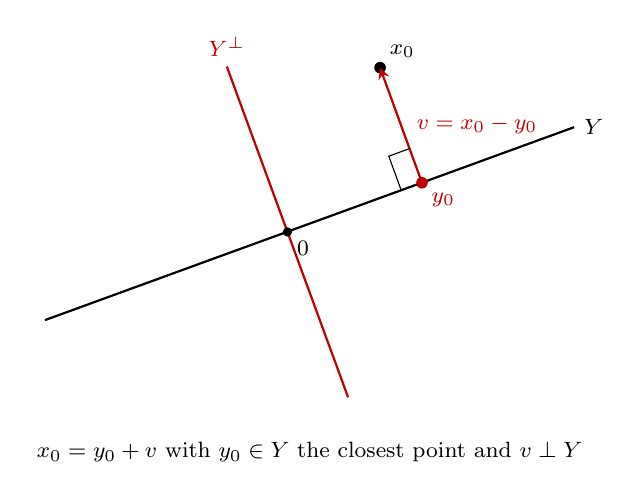
\begin{tikzpicture}[scale=1.4, >=stealth]
    \draw[thick] (-2.2,-0.8) -- (2.6,0.95) node[right, font=\footnotesize] {$Y$};
    \draw[thick, red!75!black] (0.55,-1.5) -- (-0.55,1.5) node[above, font=\footnotesize] {$Y^\perp$};
    \fill (0,0) circle (1.2pt) node[below right, font=\footnotesize] {$0$};
    % y0 on Y: direction (2.6,0.95)/|..| ; take y0 = 1.3*(0.939,0.343)
    \coordinate (Y0) at (1.22,0.446);
    \coordinate (X0) at (0.84,1.49);
    \fill (X0) circle (1.5pt) node[above right, font=\footnotesize] {$x_0$};
    \fill[red!75!black] (Y0) circle (1.5pt) node[below right, font=\footnotesize] {$y_0$};
    \draw[dashed] (X0) -- (Y0);
    \draw[->, thick, red!75!black] (Y0) -- (X0) node[midway, right, font=\footnotesize, xshift=2pt] {$v = x_0 - y_0$};
    % right angle marker at y0
    \draw[thin] ($(Y0)+(-0.113,0.31)$) -- ($(Y0)+(-0.113-0.188,0.31-0.069)$) -- ($(Y0)+(-0.188,-0.069)$);
    \node[font=\footnotesize] at (0.2,-2.0) {$x_0 = y_0 + v$ with $y_0 \in Y$ the closest point and $v \perp Y$};
\end{tikzpicture}
\end{center}

\begin{proof}
\textbf{(1), existence.} Since $Y$ is a linear subspace it is convex, and it is closed by hypothesis. By Theorem~\ref{thm:projection} there is a unique $y_0 \in Y$ with $\|x_0 - y_0\| = \operatorname{dist}(x_0, Y)$. Put $v = x_0 - y_0$, so $x_0 = y_0 + v$. It remains to show $v \in Y^\perp$, i.e.\ $(v, y) = 0$ for every $y \in Y$.

\emph{Perturbing the minimizer.} Fix $y \in Y$ and $t \in \mathbb{F}$. Since $y_0 + ty \in Y$ (a subspace), the minimality of $y_0$ gives
\[
\|v\|^2 = \|x_0 - y_0\|^2 \le \|x_0 - (y_0 + ty)\|^2 = \|v - ty\|^2 .
\]
Expanding the right side by \eqref{eq:cs-expand} with $-t$ in place of $t$,
\[
\|v - ty\|^2 = \|v\|^2 - 2\operatorname{Re}\bigl( \bar{t}\,(v, y) \bigr) + |t|^2\|y\|^2 ,
\]
so, for all $t \in \mathbb{F}$,
\begin{equation}\label{eq:perturb}
|t|^2 \|y\|^2 - 2\operatorname{Re}\bigl( \bar{t}\,(v,y) \bigr) \ge 0 .
\end{equation}

\emph{Choosing $t$.} Suppose $(v, y) \neq 0$; then $y \neq 0$. Write $(v, y) = e^{i\theta}\,|(v,y)|$ and take $t = s\,e^{i\theta}$ with $s > 0$ real, so that $\bar{t}\,(v,y) = s\,|(v,y)|$ is real and \eqref{eq:perturb} reads
\[
s^2\|y\|^2 - 2s\,|(v,y)| \ge 0, \qquad \text{i.e.} \qquad s\,\|y\|^2 \ge 2\,|(v,y)| .
\]
This fails for $0 < s < 2|(v,y)| / \|y\|^2$ --- explicitly, $s = |(v,y)|/\|y\|^2$ gives $s^2\|y\|^2 - 2s|(v,y)| = -|(v,y)|^2/\|y\|^2 < 0$ --- a contradiction. Hence $(v, y) = 0$ for every $y \in Y$, and $v \in Y^\perp$. (Wu: ``you are required to write down precisely how small is enough.'')

\textbf{(1), uniqueness.} Suppose $x = y + v = y' + v'$ with $y, y' \in Y$ and $v, v' \in Y^\perp$. Then $y - y' = v' - v$ lies in $Y \cap Y^\perp$ (both are subspaces, Proposition~\ref{prop:perp-closed}). But if $w \in Y \cap Y^\perp$ then $(w, w) = 0$ by definition of $Y^\perp$ with $w$ as the element of $Y$, so $w = 0$ by positivity. Hence $y = y'$ and $v = v'$.

\textbf{(2).} $Y \subset (Y^\perp)^\perp$ is the definition: an element of $Y$ is orthogonal to every element of $Y^\perp$. Conversely let $x \in (Y^\perp)^\perp$. By (1), $x = y + v$ with $y \in Y$, $v \in Y^\perp$. Take the inner product with $v$:
\[
(x, v) = (y, v) + (v, v) = 0 + (v, v),
\]
using $y \perp v$. But $(x, v) = 0$, because $x \in (Y^\perp)^\perp$ and $v \in Y^\perp$. So $(v, v) = 0$, $v = 0$, and $x = y \in Y$.
\end{proof}

\begin{rembox}[The Promise of Lecture 1 is Kept]\label{rem:promise-lecture-1-kept}
Corollary~\ref{cor:orth} (Lecture 1) said: \emph{if} $X = Y + Y^\perp$, then $Y^\perp$ is a complement of $Y$ and $X/Y \cong Y^\perp$. The theorem just proved supplies the hypothesis for every closed subspace of a Hilbert space, so in that setting the quotient $X/Y$ really is the orthogonal complement, as the picture in \S\ref{subsec:quotient} suggested; the remark following Corollary~\ref{cor:orth} identified exactly this theorem as the missing piece. The hypotheses are sharp: $c_{00} \subset \ell^2$ (not closed) has $c_{00}^\perp = \{0\}$, so $c_{00} + c_{00}^\perp \neq \ell^2$, while $(c_{00}^\perp)^\perp = \ell^2 \neq c_{00}$ --- both (1) and (2) fail. For an arbitrary subset $M$, $(M^\perp)^\perp = \overline{\operatorname{span}}\, M$ (Theorem~\ref{thm:double-perp}).
\end{rembox}

\begin{rembox}\label{rem:projection-2}
The proof of (1) is the first-variation argument of calculus, in the form ``at a minimum the derivative vanishes'': $y_0$ minimizes $y \mapsto \|x_0 - y\|^2$ over $Y$, so moving $y_0$ along any direction $y \in Y$ cannot decrease the value, and \eqref{eq:perturb} is the statement that the linear term in $t$ of the expansion must vanish. The rotation $t = s e^{i\theta}$ is Technique~8 again. Riesz's lemma (Lemma~\ref{lem:riesz}) was the substitute for this argument in a bare normed space; here the constant $\tfrac12$ improves to an exact orthogonal vector, as the remark after Proposition~\ref{prop:riesz-sharp} anticipated.
\end{rembox}


\subsection{The Double Complement}

\begin{lembox}[A Set and Its Closed Span Have the Same Complement]\boxlabel{lem:perp-span}
For any subset $M$ of an inner product space $X$, $M^\perp = \bigl( \overline{\operatorname{span}}\, M \bigr)^\perp$.
\end{lembox}

\begin{proof}
(HW4, Problem 2, Step 1.) Let $Y = \overline{\operatorname{span}}\, M$. Since $M \subset Y$, every vector orthogonal to $Y$ is orthogonal to $M$. Conversely, let $v \in M^\perp$. For a finite combination $z = \sum_i a_i m_i$ with $m_i \in M$, $(z, v) = \sum_i a_i (m_i, v) = \sum_i a_i\,\overline{(v, m_i)} = 0$, so $v \perp \operatorname{span} M$; and if $z_n \to y$ with $z_n \in \operatorname{span} M$, then $(y, v) = \lim_n (z_n, v) = 0$ by Lemma~\ref{lem:ip-continuous}. So $v \in Y^\perp$.
\end{proof}

\begin{thmbox}[The Double Complement]\boxlabel{thm:double-perp}
For any subset $M$ of a Hilbert space $H$,
\[
(M^\perp)^\perp = \overline{\operatorname{span}}\, M .
\]
In particular $M^\perp = \{0\}$ if and only if $\operatorname{span} M$ is dense in $H$.
\laxref{\S6.4, Thm~7}
\end{thmbox}

\begin{proof}
(HW4, Problem 2.) $Y = \overline{\operatorname{span}}\, M$ is a closed linear subspace (Definition~\ref{def:closed-span}). By Lemma~\ref{lem:perp-span} and Theorem~\ref{thm:orth-decomp}(2),
\[
(M^\perp)^\perp = (Y^\perp)^\perp = Y .
\]
For the last statement: if $M^\perp = \{0\}$ then $Y = \{0\}^\perp = H$; conversely, if $Y = H$ then $M^\perp = Y^\perp = H^\perp = \{0\}$, since a vector orthogonal to itself is $0$.
\end{proof}

\begin{rembox}\label{rem:projection-3}
Without completeness only one inclusion survives: $\overline{\operatorname{span}}\, M \subset (M^\perp)^\perp$ holds in any inner product space, because $(M^\perp)^\perp$ is a closed subspace (Proposition~\ref{prop:perp-closed}) containing $M$. The reverse inclusion is where Theorem~\ref{thm:orth-decomp}(2), and hence completeness, is used. The last statement of the theorem is the general form of Proposition~\ref{prop:lax-onb}: an orthonormal set is complete exactly when its span is dense.
\end{rembox}

\subsection{Example: Even and Odd Functions}

\begin{propbox}[Even and Odd Functions]\boxlabel{prop:even-odd}
In $L^2[-1,1]$ let $E$ be the set of even functions ($f(-x) = f(x)$ a.e.) and $O$ the set of odd functions ($f(-x) = -f(x)$ a.e.). Then:
\begin{enumerate}[label=(\alph*)]
    \item $E^\perp = O$ and $O^\perp = E$;
    \item $E$ and $O$ are closed subspaces, and $L^2[-1,1] = E \oplus O$: every $f$ is uniquely $f = f_e + f_o$ with
    \[
    f_e(x) = \tfrac12\bigl( f(x) + f(-x) \bigr) \in E, \qquad f_o(x) = \tfrac12\bigl( f(x) - f(-x) \bigr) \in O ,
    \]
    and $f_e$ is the closest point of $E$ to $f$.
\end{enumerate}
\end{propbox}

\begin{proof}
(HW4, Problem 1, for $E^\perp = O$.) 
Throughout, $\mathbb{F}$ is $\mathbb{R}$ or $\mathbb{C}$, $L^2 = L^2[-1,1]$ with $(f,g) = \int_{-1}^1 f\,\bar{g}\,dx$, and elements of $L^2$ are functions up to equality almost everywhere. A function $f \in L^2$ is \emph{even} if $f(-x) = f(x)$ for a.e.\ $x$, and \emph{odd} if $f(-x) = -f(x)$ for a.e.\ $x$. We show that
\[S^\perp = \{ g \in L^2[-1,1] : g \text{ is odd} \}.\]
We use one fact from real analysis: Lebesgue measure on $[-1,1]$ is invariant under $x \mapsto -x$, so for integrable $h$, $\int_{-1}^1 h(-x)\,dx = \int_{-1}^1 h(x)\,dx$, and $x \mapsto -x$ maps null sets to null sets.

\textbf{Step 1: the reflection.} For $f \in L^2$ put $(Rf)(x) = f(-x)$. This is well defined on classes (reflection preserves null sets), $Rf \in L^2$ with $\int |Rf|^2 = \int |f|^2$, and $R$ is linear with $R(Rf) = f$. By definition, $f$ is even iff $Rf = f$ and odd iff $Rf = -f$. For $f \in L^2$ put
\[f_e = \tfrac12 (f + Rf), \qquad f_o = \tfrac12 (f - Rf).\]
Then $f_e, f_o \in L^2$, $f = f_e + f_o$, $R f_e = \tfrac12(Rf + f) = f_e$ and $R f_o = \tfrac12(Rf - f) = -f_o$; so $f_e$ is even and $f_o$ is odd.

\textbf{Step 2: odd functions lie in $S^\perp$.} Let $f \in S$ and $g$ odd. The function $h = f\bar{g}$ is integrable (by the Cauchy--Schwarz inequality in $L^2$) and $h(-x) = f(-x)\overline{g(-x)} = -f(x)\overline{g(x)} = -h(x)$ for a.e.\ $x$. By reflection invariance,
\[(f, g) = \int_{-1}^1 h(x)\,dx = \int_{-1}^1 h(-x)\,dx = -\int_{-1}^1 h(x)\,dx = -(f, g),\]
so $(f, g) = 0$. Hence $g \in S^\perp$. By the conjugate symmetry $(g,f) = \overline{(f,g)}$, also $(g, f) = 0$.

\textbf{Step 3: every element of $S^\perp$ is odd.} Let $g \in S^\perp$ and write $g = g_e + g_o$ as in Step 1. Since $g_e \in S$, the definition of $S^\perp$ gives $(g, g_e) = 0$. On the other hand, by Step 2 (with $f = g_e$ even and $g_o$ odd), $(g_o, g_e) = 0$, so
\[0 = (g, g_e) = (g_e, g_e) + (g_o, g_e) = \|g_e\|^2 .\]
Hence $g_e = 0$ in $L^2$, i.e.\ $g = g_o$ is odd.

By Steps 2 and 3, $E^\perp = O$.


\textbf{Step 4: $O^\perp = E$.} By Step 2 every even function is orthogonal to every odd function, so $E \subset O^\perp$. If $g \in O^\perp$, write $g = g_e + g_o$; since $g_o \in O$, $0 = (g, g_o) = (g_e, g_o) + (g_o, g_o) = \|g_o\|^2$, so $g = g_e \in E$. (Not part of the homework.)

\textbf{Step 5: (b).} By (a) and Proposition~\ref{prop:perp-closed}, $E = O^\perp$ and $O = E^\perp$ are closed subspaces. The decomposition $f = f_e + f_o$ of Step 1 has $f_e \in E$ and $f_o \in O = E^\perp$, so it is the decomposition of Theorem~\ref{thm:orth-decomp} for $Y = E$; its uniqueness is part of that theorem, and $f_e$ is the closest point of $E$ to $f$ by the proof of that theorem. (Not part of the homework.)
\end{proof}

\begin{center}
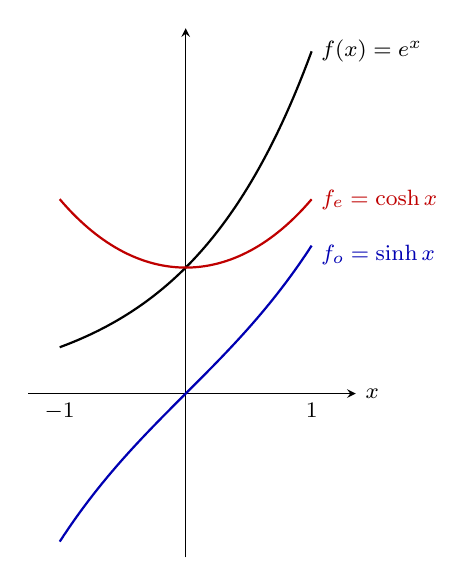
\begin{tikzpicture}[scale=1.6, >=stealth]
    \draw[->] (-1.25,0) -- (1.35,0) node[right] {$x$};
    \draw[->] (0,-1.3) -- (0,2.9);
    \draw[thick, domain=-1:1, samples=60] plot (\x, {exp(\x)});
    \draw[thick, red!75!black, domain=-1:1, samples=60] plot (\x, {cosh(\x)});
    \draw[thick, blue!70!black, domain=-1:1, samples=60] plot (\x, {sinh(\x)});
    \node[right] at (1,2.72) {$f(x) = e^x$};
    \node[right, red!75!black] at (1,1.54) {$f_e = \cosh x$};
    \node[right, blue!70!black] at (1,1.1) {$f_o = \sinh x$};
    \node[below] at (-1,0) {$-1$};
    \node[below] at (1,0) {$1$};
\end{tikzpicture}
\end{center}
For $f(x) = e^x$ the decomposition is $e^x = \cosh x + \sinh x$: the even part is the orthogonal projection of $e^x$ onto $E$, and the odd part is orthogonal to every even function.

\subsection{An Application: A Sharp Integral Inequality}

\begin{propbox}[A Sharp Integral Inequality]\boxlabel{prop:sharp-integral}
Let $f \in C^2([a,b])$ with $f(a) = f(b) = 0$, $f'(a) = 1$, $f'(b) = 0$, and $L = b - a$. Then
\[
\int_a^b |f''(x)|^2\,dx \ge \frac{4}{L},
\]
with equality for $f_*(x) = (x - a)\bigl( 1 - \tfrac{x-a}{L} \bigr)^2$.
\end{propbox}

\begin{proof}
(HW4, Problem 4.) 
Write $L = b - a > 0$. Functions may be real or complex valued; all integrals are Riemann integrals of continuous functions. We use the Cauchy--Schwarz inequality for the inner product $(u, v) = \int_a^b u\,\bar{v}\,dx$ on $C([a,b])$ (the restriction of the $L^2$ inner product; Theorem~\ref{thm:cauchy-schwarz}).

\textbf{Step 1: an identity for $f''$.} Let $g(x) = 1 - \dfrac{3(x - a)}{2L}$, a real polynomial with $g(a) = 1$ and $g'(x) = -\dfrac{3}{2L}$. Since $f' \in C^1([a,b])$ and $g \in C^1([a,b])$, integration by parts gives
\[\int_a^b f''(x)\,g(x)\,dx = \bigl[ f'(x)\,g(x) \bigr]_a^b - \int_a^b f'(x)\,g'(x)\,dx .\]
The boundary term is $f'(b)g(b) - f'(a)g(a) = 0 \cdot g(b) - 1 \cdot 1 = -1$. Since $g'$ is the constant $-\frac{3}{2L}$, the fundamental theorem of calculus gives
\[\int_a^b f'(x)\,g'(x)\,dx = -\frac{3}{2L}\bigl( f(b) - f(a) \bigr) = 0 .\]
Hence
\[\int_a^b f''(x)\,g(x)\,dx = -1 .\]

\textbf{Step 2: the norm of $g$.} With $t = x - a$,
\[\int_a^b |g(x)|^2\,dx = \int_0^L \Bigl( 1 - \frac{3t}{2L} \Bigr)^2 dt = \int_0^L \Bigl( 1 - \frac{3t}{L} + \frac{9t^2}{4L^2} \Bigr) dt = L - \frac{3L}{2} + \frac{3L}{4} = \frac{L}{4} .\]

\textbf{Step 3: Cauchy--Schwarz.} Since $g$ is real, $\int_a^b f'' g\,dx = (f'', g)$. By Step 1 and Cauchy--Schwarz,
\[1 = \bigl| (f'', g) \bigr| \le \Bigl( \int_a^b |f''|^2\,dx \Bigr)^{1/2} \Bigl( \int_a^b |g|^2\,dx \Bigr)^{1/2} = \Bigl( \int_a^b |f''|^2\,dx \Bigr)^{1/2} \sqrt{\frac{L}{4}} .\]
Squaring and rearranging,
\[\int_a^b |f''(x)|^2\,dx \ge \frac{4}{L} = \frac{4}{b - a}. \qedhere\]


\textbf{Step 4: sharpness.} (Not part of the homework.) Let $f_*(x) = (x - a)\bigl(1 - \frac{x - a}{L}\bigr)^2$. With $t = x - a$, $f_* = t - \frac{2t^2}{L} + \frac{t^3}{L^2}$, so $f_*(a) = 0$ and $f_*(b) = L - 2L + L = 0$; $f_*' = 1 - \frac{4t}{L} + \frac{3t^2}{L^2}$ equals $1$ at $t = 0$ and $1 - 4 + 3 = 0$ at $t = L$; and $f_*'' = -\frac{4}{L} + \frac{6t}{L^2} = -\frac{4}{L}\,g$. Hence, by Step 2,
\[
\int_a^b |f_*''|^2\,dx = \frac{16}{L^2} \int_a^b g^2\,dx = \frac{16}{L^2} \cdot \frac{L}{4} = \frac{4}{L}. \qedhere
\]
\end{proof}

\begin{rembox}[Where $g$ Comes From]\label{rem:where-g-comes}
The boundary conditions fix two inner products of $h = f''$ with fixed functions: $\int_a^b h = f'(b) - f'(a) = -1$, and, by Taylor's formula with integral remainder, $\int_a^b (b - x)\,h(x)\,dx = f(b) - f(a) - f'(a)L = -L$. Let $Y = \operatorname{span}\{1, x\}$, a closed (finite-dimensional) subspace of $L^2[a,b]$, and decompose $h = h_Y + h_\perp$ with $h_Y \in Y$, $h_\perp \perp Y$. The two constraints involve only $h_Y$, while $\|h\|^2 = \|h_Y\|^2 + \|h_\perp\|^2 \ge \|h_Y\|^2$ by Pythagoras. So the minimum of $\|h\|$ under the constraints is attained by an element of $Y$ --- a linear function --- and that is why testing against a linear $g$ loses nothing. This is the projection theorem at work: the constraint set is a closed affine subspace, and its point closest to $0$ lies in the orthogonal complement of the directions along it. It is also a first example of the calculus of variations recast in a Hilbert space.
\end{rembox}

% ============================================================================
% SECTION 19: BOUNDED LINEAR FUNCTIONALS AND RIESZ REPRESENTATION
% ============================================================================

\section{Bounded Linear Functionals and the Riesz Representation Theorem}\label{sec:riesz-rep}

\roadmark{Stage: inner products}{Thread: functionals. On a Hilbert space every bounded functional is an inner product.}

\subsection{Bounded Linear Functionals}

On $\mathbb{R}^n$ every linear functional is $x \mapsto a \cdot x$ for a unique vector $a$ (Example~\ref{ex:functionals-rn}). The Riesz representation theorem says the same is true in any Hilbert space, once ``linear functional'' is replaced by the right notion.

\begin{defbox}[Bounded Linear Functional]\boxlabel{def:bounded-functional}
Let $(X, \|\cdot\|)$ be a normed linear space over $\mathbb{F}$. A linear functional $\ell : X \to \mathbb{F}$ is \textbf{bounded} if there is a constant $c > 0$ such that
\[
|\ell(x)| \le c\,\|x\| \qquad \text{for all } x \in X .
\]
\laxref{\S6.3, (14)}
\end{defbox}

\begin{rembox}[Why Boundedness]\label{rem:why-boundedness}
On $\mathbb{R}^n$ every linear functional is bounded: $|a \cdot x| \le \|a\|\,\|x\|$ by Cauchy--Schwarz, so $c = \|a\|$ works. More generally every linear functional on a finite-dimensional normed space is bounded (with a basis $e_1, \ldots, e_n$ and $x = \sum_i a_i e_i$, $|\ell(x)| \le \sum_i |a_i|\,|\ell(e_i)| \le \bigl(\max_i |\ell(e_i)|\bigr)\|x\|_1$, and $\|\cdot\|_1$ is equivalent to the given norm by Theorem~\ref{prop:norms-equiv}). In infinite dimensions this fails --- the remark after Proposition~\ref{prop:norm-continuous} and the remark after Theorem~\ref{thm:jvn} both mention functionals built from a Hamel basis that are unbounded on every ball --- so boundedness is a genuine hypothesis, and it is the one that makes the finite-dimensional picture survive. ``Bounded'' does not mean bounded as a function: a nonzero linear functional is never bounded on all of $X$, since $\ell(nx) = n\ell(x)$; it means bounded on the unit ball.
\end{rembox}

\begin{propbox}[Bounded Means Continuous]\boxlabel{prop:bounded-continuous}
For a linear functional $\ell$ on a normed linear space $X$, the following are equivalent:
\begin{enumerate}[label=(\roman*)]
    \item $\ell$ is bounded;
    \item $\ell$ is continuous on $X$ (if $x_n \to x$ then $\ell(x_n) \to \ell(x)$);
    \item $\ell$ is continuous at $0$.
\end{enumerate}
\end{propbox}

\begin{proof}
(Not covered in lecture.) (i)$\Rightarrow$(ii): $|\ell(x_n) - \ell(x)| = |\ell(x_n - x)| \le c\|x_n - x\| \to 0$. (ii)$\Rightarrow$(iii) is trivial. (iii)$\Rightarrow$(i): if $\ell$ is not bounded, then for each $n$ there is $x_n$ with $|\ell(x_n)| > n\|x_n\|$, so $x_n \neq 0$; put $z_n = x_n / (n\|x_n\|)$. Then $\|z_n\| = 1/n \to 0$, so $z_n \to 0$, while $|\ell(z_n)| = |\ell(x_n)| / (n\|x_n\|) > 1$, so $\ell(z_n) \not\to 0 = \ell(0)$, contradicting (iii).
\end{proof}

\subsection{The Riesz Representation Theorem}

\begin{thmbox}[Riesz Representation Theorem]\boxlabel{thm:riesz-rep}
Let $H$ be a Hilbert space over $\mathbb{F}$.
\begin{enumerate}[label=(\arabic*)]
    \item For every $a \in H$, the map $\ell_a : H \to \mathbb{F}$, $\ell_a(x) = (x, a)$, is a bounded linear functional on $H$.
    \item Conversely, for every bounded linear functional $\ell : H \to \mathbb{F}$ there is a unique $a \in H$ such that
    \[
    \ell(x) = (x, a) \qquad \text{for all } x \in H .
    \]
\end{enumerate}
\laxref{\S6.3, Thm~4}
\end{thmbox}

\begin{rembox}[Reading the Statement]\label{rem:reading-statement-2}
Part (1) is the easy direction and holds in any inner product space. Part (2) is the content: on a Hilbert space there are \emph{no other} bounded linear functionals than the ones given by inner products, exactly as on $\mathbb{R}^n$. Wu's example: on $L^2$, every bounded linear functional is $f \mapsto \int f\,\bar{g}$ for a unique $g \in L^2$. The vector is on the \emph{second} slot because the functional must be linear in $x$, and the inner product is linear in its first argument; with the physicists' convention it would be $(a, x)$.
\end{rembox}

\begin{proof}[Proof of (1)]
Linearity of $\ell_a$ in $x$ is linearity of the inner product in its first argument. Boundedness is Cauchy--Schwarz (Theorem~\ref{thm:cauchy-schwarz}): $|\ell_a(x)| = |(x, a)| \le \|a\|\,\|x\|$, so $c = \|a\|$ works.
\end{proof}

% Lecture 8 (2026-09-24)
The idea of the proof comes from $\mathbb{R}^n$: there $\ell(x) = x \cdot a$, the set $\{\ell = 0\}$ is a hyperplane, and $a$ is a normal vector to it. So one studies the null set of $\ell$ and looks for a vector perpendicular to it. Two facts about the null set are needed first; they are separated out as lemmas.

\begin{lembox}[The Kernel of a Bounded Functional is Closed]\boxlabel{lem:kernel-closed}
Let $\ell$ be a bounded linear functional on a normed linear space $X$. Then its \textbf{kernel} (or null set)
\[
N = \ker \ell = \{ y \in X : \ell(y) = 0 \}
\]
is a closed linear subspace of $X$.
\end{lembox}

\begin{proof}
\emph{Subspace.} If $y_1, y_2 \in N$ and $a, b \in \mathbb{F}$, then $\ell(ay_1 + by_2) = a\ell(y_1) + b\ell(y_2) = 0$.

\emph{Closed.} Let $y_n \in N$ with $y_n \to y_0$. Since $\ell$ is bounded, $|\ell(x)| \le M\|x\|$ for some $M$ and all $x$, so
\[
|\ell(y_n) - \ell(y_0)| = |\ell(y_n - y_0)| \le M\|y_n - y_0\| \to 0 .
\]
As $\ell(y_n) = 0$ for all $n$, this gives $\ell(y_0) = 0$, i.e.\ $y_0 \in N$.
\end{proof}

This is the only place in the proof where boundedness is used; by Proposition~\ref{prop:bounded-continuous} it amounts to continuity of $\ell$.

\begin{lembox}[The Kernel Has Codimension One]\boxlabel{lem:ker-codim1}
Let $H$ be a Hilbert space, $\ell \neq 0$ a bounded linear functional on $H$, and $N = \ker \ell$. Then $N^\perp \neq \{0\}$, and for every nonzero $x_0 \in N^\perp$:
\begin{enumerate}[label=(\alph*)]
    \item $\ell(x_0) \neq 0$;
    \item $N^\perp = \{ k x_0 : k \in \mathbb{F} \}$, so $N^\perp$ is one-dimensional;
    \item every $x \in H$ can be written as $x = k x_0 + y$ with $k = \ell(x)/\ell(x_0) \in \mathbb{F}$ and $y \in N$.
\end{enumerate}
\laxref{\S6.3, Lemma~5(i)}
\end{lembox}

\begin{proof}
By Lemma~\ref{lem:kernel-closed}, $N$ is a closed linear subspace, and $N \neq H$ because $\ell \neq 0$. By Theorem~\ref{thm:orth-decomp}, $H = N \oplus N^\perp$; if $N^\perp$ were $\{0\}$ this would give $H = N$. So $N^\perp \neq \{0\}$. Fix $0 \neq x_0 \in N^\perp$.

(a) If $\ell(x_0) = 0$ then $x_0 \in N \cap N^\perp = \{0\}$ (a vector orthogonal to itself is $0$), contrary to the choice of $x_0$.

(b) Let $x_1 \in N^\perp$ and put $k = \ell(x_1)/\ell(x_0)$, a quotient of two scalars, so $k \in \mathbb{F}$. Then $\ell(x_1) = k\,\ell(x_0)$, so $\ell(x_1 - k x_0) = 0$ and $x_1 - k x_0 \in N$. But also $x_1 - k x_0 \in N^\perp$, a linear subspace (Proposition~\ref{prop:perp-closed}). Hence $x_1 - k x_0 \in N \cap N^\perp = \{0\}$, i.e.\ $x_1 = k x_0$. Conversely every $k x_0$ lies in $N^\perp$.

(c) With $k = \ell(x)/\ell(x_0)$ and $y = x - k x_0$, linearity gives $\ell(y) = \ell(x) - k\,\ell(x_0) = 0$, so $y \in N$.
\end{proof}

\begin{rembox}\label{rem:riesz-rep}
Two points raised in lecture. The step $k = \ell(x_1)/\ell(x_0)$ may look like dividing vectors, but it is not: $\ell(x_1)$ and $\ell(x_0)$ are numbers, and the vector identity $x_1 = kx_0$ is obtained afterwards from $N \cap N^\perp = \{0\}$. And a student asked why this shows $\dim N^\perp = 1$: an arbitrary element $x_1$ of $N^\perp$ was shown to be a multiple of one fixed nonzero $x_0$.
\end{rembox}

\begin{proof}[Proof of (2)]
If $\ell = 0$, then $\ell(x) = (x, 0)$ for all $x$, so $a = 0$ works. Assume $\ell \neq 0$, let $N = \ker \ell$, and fix $0 \neq x_0 \in N^\perp$ (Lemma~\ref{lem:ker-codim1}).

\emph{Finding $a$.} Consider the bounded linear functional $\ell_1(x) = (x, x_0)$. For $x = k x_0 + y$ as in Lemma~\ref{lem:ker-codim1}(c),
\[
\ell_1(x) = k(x_0, x_0) + (y, x_0) = k\,\|x_0\|^2, \qquad \ell(x) = k\,\ell(x_0) + \ell(y) = k\,\ell(x_0),
\]
since $(y, x_0) = 0$ ($y \in N$, $x_0 \in N^\perp$) and $\ell(y) = 0$. The two differ by the constant factor $\ell(x_0)/\|x_0\|^2$. This suggests
\[
a = \frac{\overline{\ell(x_0)}}{\|x_0\|^2}\, x_0 ,
\]
the conjugate being needed because the inner product is conjugate-linear in its second argument.

\emph{Verification.} For $x = k x_0 + y$ as above, using $(x, c\,x_0) = \bar{c}\,(x, x_0)$,
\[
(x, a) = \frac{\ell(x_0)}{\|x_0\|^2}\,(k x_0 + y,\, x_0) = \frac{\ell(x_0)}{\|x_0\|^2}\, k\,\|x_0\|^2 = k\,\ell(x_0) = \ell(x).
\]

\emph{Uniqueness.} If $(x, a) = (x, a')$ for all $x \in H$, then $(x, a - a') = 0$ for all $x$; taking $x = a - a'$ gives $\|a - a'\|^2 = 0$, so $a = a'$. (Not written out in lecture.)
\end{proof}

\begin{center}
\begin{tikzpicture}[scale=1.3, >=stealth]
    \draw[thick] (-2.2,0) -- (3.0,0) node[right, font=\footnotesize] {$N = \ker \ell = \{\ell = 0\}$};
    \draw[dashed, gray] (-2.2,1.3) -- (3.0,1.3);
    \node[left, font=\footnotesize] at (-2.2,1.3) {$\{\ell = \ell(x)\}$};
    \draw[thin] (0,-0.7) -- (0,2.0) node[above, font=\footnotesize] {$N^\perp$};
    \fill (0,0) circle (1.2pt) node[below left, font=\footnotesize] {$0$};
    \draw[->, thick, blue!70!black] (0,0) -- (0,0.95);
    \node[right, font=\footnotesize, blue!70!black] at (0.03,0.9) {$a$};
    \draw[->, thick, red!75!black] (0,0) -- (0,0.5);
    \node[left, font=\footnotesize, red!75!black] at (-0.03,0.4) {$x_0$};
    \fill (2.0,1.3) circle (1.5pt) node[above, font=\footnotesize, yshift=1pt] {$x = kx_0 + y$};
    \draw[dashed] (2.0,1.3) -- (2.0,0);
    \draw[dashed] (2.0,1.3) -- (0,1.3);
    \fill (2.0,0) circle (1.2pt) node[below, font=\footnotesize] {$y \in N$};
    \fill (0,1.3) circle (1.2pt) node[above left, font=\footnotesize] {$kx_0$};
    \draw[thin] (0,0.15) -- (0.15,0.15) -- (0.15,0);
\end{tikzpicture}
\end{center}
The null set $N$ is a closed hyperplane and $N^\perp$ a line; $a$ is a normal vector to $N$, a multiple of $x_0$. The level sets $\{\ell = c\}$ are the translates of $N$, and $\ell(x)$ records only which translate $x$ lies on, i.e.\ the $N^\perp$-component $kx_0$ of $x$.

\begin{rembox}\label{rem:riesz-rep-2}
Wu on method: ``when we try to prove a big theorem, very often the simple examples we learned, like in linear algebra, give the answer; start with simple examples and go from there.'' Here the finite-dimensional picture dictated both the object to study ($\ker \ell$) and the candidate ($a$ normal to it); the analysis consisted of making the orthogonal decomposition available, which is where completeness of $H$ and boundedness of $\ell$ enter.
\end{rembox}

\begin{rembox}[Comparison with Lax]\label{rem:comparison-lax-6}
Lax proves the representation theorem through his Lemma~5: the null space of a nonzero functional has codimension one, and two functionals with the same null space are proportional. He takes $z \neq 0$ in $N^\perp$ and observes that $\ell$ and $x \mapsto (x, z)$ have the same null space, so $\ell$ is a multiple of $(\cdot, z)$. Wu's proof (Lemma~\ref{lem:ker-codim1} and the explicit decomposition $x = kx_0 + y$) is the same argument with the proportionality constant computed by hand.
\end{rembox}

% ============================================================================
% SECTION 20: ORTHONORMAL SETS AND BASES
% ============================================================================
% Lecture 8 (2026-09-24)

\section{Orthonormal Sets and Bases}\label{sec:onb}

\roadmark{Stage: inner products}{Threads: dimension, completeness. Countable support, Bessel and Parseval: bases in infinite dimensions.}

\subsection{Orthonormal Sets}

\begin{defbox}[Orthogonal and Orthonormal Sets]\boxlabel{def:onset}
Let $X$ be an inner product space and $\{e_\alpha\}_{\alpha \in \Lambda} \subset X$, indexed by an arbitrary set $\Lambda$. The family is \textbf{orthogonal} if $e_\alpha \perp e_\beta$ for all $\alpha, \beta \in \Lambda$ with $\alpha \neq \beta$. It is \textbf{orthonormal} if in addition $\|e_\alpha\| = 1$ for every $\alpha \in \Lambda$.
\laxref{\S6.4, definition of orthonormal set}
\end{defbox}

\begin{defbox}[Complete Orthogonal Set]\boxlabel{def:complete-onset}
An orthogonal set $\{e_\alpha\}_{\alpha \in \Lambda}$ in $X$ is \textbf{complete} if the only vector orthogonal to all of its members is $0$:
\[
(x, e_\alpha) = 0 \ \text{ for all } \alpha \in \Lambda \quad \Longrightarrow \quad x = 0 .
\]
\end{defbox}

\begin{rembox}\label{rem:onb}
Completeness of an orthogonal set is unrelated to completeness of a space. It means the set cannot be enlarged: if some nonzero $x$ were orthogonal to every $e_\alpha$, it could be added to the set, which therefore could not be a basis. In $\mathbb{R}^n$, a complete orthonormal set $\{e_1, \ldots, e_n\}$ is a basis, and every $x$ is $x = \sum_{j=1}^n (x, e_j)\, e_j$. The question is whether the same is true in a Hilbert space.
\end{rembox}

\begin{rembox}[What Should ``Basis'' Mean]\label{rem:what-should-basis-mean}
The natural definition is that every $x \in H$ satisfies $x = \sum_{\alpha \in \Lambda} (x, e_\alpha)\, e_\alpha$. But the right side need not make sense a priori. Adding finitely many vectors is part of the linear structure; adding infinitely many requires a limit (compare the remark on finite sums in \S\ref{subsec:span}); and $\Lambda$ may be uncountable, in which case it is not even clear in what order to add. The following results make sense of it in three steps: for each $x$ only countably many coefficients $(x, e_\alpha)$ are nonzero; the sum of their squares is at most $\|x\|^2$ (Bessel); and the vector series then converges in $H$. Only the last step uses completeness of $H$; the first two hold in any inner product space.
\end{rembox}

\subsection{Pythagoras and Bessel's Inequality}

\begin{lembox}[Pythagoras]\boxlabel{lem:pythagoras}
Let $X$ be an inner product space.
\begin{enumerate}[label=(\alph*)]
    \item If $u \perp v$, then $\|u + v\|^2 = \|u\|^2 + \|v\|^2$.
    \item If $e_1, \ldots, e_k$ are orthonormal and $c_1, \ldots, c_k \in \mathbb{F}$, then $\bigl\| \sum_{j=1}^k c_j e_j \bigr\|^2 = \sum_{j=1}^k |c_j|^2$.
\end{enumerate}
\end{lembox}

\begin{proof}
(a) By \eqref{eq:cs-expand} with $t = 1$, $\|u + v\|^2 = \|u\|^2 + 2\operatorname{Re}(v, u) + \|v\|^2$, and $(v, u) = 0$.

(b) Induction on $k$; the case $k = 1$ is $\|c_1 e_1\|^2 = |c_1|^2$. For the step, $u = \sum_{j < k} c_j e_j$ and $v = c_k e_k$ are orthogonal, since $(u, v) = \sum_{j<k} c_j \bar{c}_k (e_j, e_k) = 0$; so by (a) and the induction hypothesis, $\|u + v\|^2 = \sum_{j<k} |c_j|^2 + |c_k|^2$.
\end{proof}

\begin{lembox}[Finite Bessel Inequality]\boxlabel{lem:finite-bessel}
Let $\{e_\alpha\}_{\alpha \in \Lambda}$ be orthonormal in an inner product space $X$, let $e_1, \ldots, e_k$ be finitely many distinct members of it, and $x \in X$. Put $y = x - \sum_{j=1}^k (x, e_j)\, e_j$. Then $y \perp e_i$ for $i = 1, \ldots, k$, and
\[
\|x\|^2 = \|y\|^2 + \sum_{j=1}^k |(x, e_j)|^2 ; \qquad \text{in particular} \qquad \sum_{j=1}^k |(x, e_j)|^2 \le \|x\|^2 .
\]
\end{lembox}

\begin{proof}
For each $i$, taking the scalars $(x, e_j)$ out of the first slot,
\[
(y, e_i) = (x, e_i) - \sum_{j=1}^k (x, e_j)\,(e_j, e_i) = (x, e_i) - (x, e_i) = 0,
\]
since $(e_j, e_i) = 0$ for $j \neq i$ and $(e_i, e_i) = 1$. Hence $y$ is orthogonal to $\sum_j (x, e_j) e_j$ (conjugate-linearity in the second slot), and $x = y + \sum_j (x, e_j) e_j$. By Lemma~\ref{lem:pythagoras}(a) and then (b), $\|x\|^2 = \|y\|^2 + \bigl\|\sum_j (x, e_j) e_j\bigr\|^2 = \|y\|^2 + \sum_j |(x, e_j)|^2$.
\end{proof}

\begin{center}
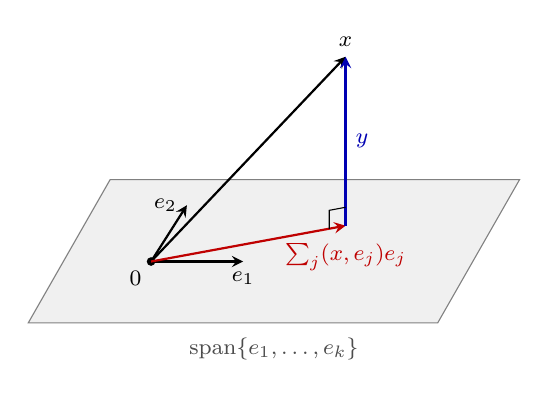
\begin{tikzpicture}[scale=1.3, >=stealth]
    % plane span{e1,e2} in perspective
    \fill[gray!12] (-1.2,-0.6) -- (2.8,-0.6) -- (3.6,0.8) -- (-0.4,0.8) -- cycle;
    \draw[thin, gray] (-1.2,-0.6) -- (2.8,-0.6) -- (3.6,0.8) -- (-0.4,0.8) -- cycle;
    \node[font=\footnotesize, gray!60!black] at (1.2,-0.85) {$\operatorname{span}\{e_1, \ldots, e_k\}$};
    \fill (0,0) circle (1.2pt) node[below left, font=\footnotesize] {$0$};
    \draw[->, thick] (0,0) -- (0.9,0) node[below, font=\footnotesize] {$e_1$};
    \draw[->, thick] (0,0) -- (0.35,0.55) node[left, font=\footnotesize] {$e_2$};
    \coordinate (P) at (1.9,0.35);
    \coordinate (X) at (1.9,2.0);
    \draw[->, thick] (0,0) -- (X) node[above, font=\footnotesize] {$x$};
    \draw[->, thick, red!75!black] (0,0) -- (P);
    \node[below, font=\footnotesize, red!75!black, yshift=-3pt] at (P) {$\sum_{j} (x, e_j) e_j$};
    \draw[->, thick, blue!70!black] (P) -- (X) node[midway, right, font=\footnotesize] {$y$};
    \draw[thin] ($(P)+(0,0.18)$) -- ($(P)+(-0.16,0.15)$) -- ($(P)+(-0.16,-0.03)$);
\end{tikzpicture}
\end{center}
The picture Wu described: $\sum_j (x, e_j) e_j$ is the orthogonal projection of $x$ onto $\operatorname{span}\{e_1, \ldots, e_k\}$, and $y$ is the perpendicular remainder. Pythagoras applied to $k + 1$ orthogonal pieces gives the identity; dropping $\|y\|^2$ gives the inequality.

\begin{defbox}[Sums of Non-Negative Families]\boxlabel{def:family-sum}
Let $(t_\alpha)_{\alpha \in \Lambda}$ be real numbers with $t_\alpha \ge 0$ whose \textbf{support} $S = \{ \alpha \in \Lambda : t_\alpha \neq 0 \}$ is countable. Define
\[
\sum_{\alpha \in \Lambda} t_\alpha := \sum_{n} t_{\alpha_n} \in [0, \infty],
\]
where $\alpha_1, \alpha_2, \ldots$ is an enumeration of $S$ (a finite sum if $S$ is finite, and $0$ if $S = \varnothing$).
\end{defbox}

\begin{lembox}[The Sum Does Not Depend on the Enumeration]\boxlabel{lem:family-sum}
In Definition~\ref{def:family-sum},
\[
\sum_{\alpha \in \Lambda} t_\alpha = \sup \Bigl\{ \sum_{\alpha \in F} t_\alpha : F \subset \Lambda \text{ finite} \Bigr\} ;
\]
in particular the sum is independent of the enumeration of $S$.
\end{lembox}

\begin{proof}
(Not covered in lecture.) Let $T$ be the supremum. Each partial sum $\sum_{n \le N} t_{\alpha_n}$ is a sum over a finite subset of $\Lambda$, so it is at most $T$, and hence so is the limit of these increasing partial sums. Conversely, for finite $F \subset \Lambda$, the finite set $F \cap S$ is contained in $\{\alpha_1, \ldots, \alpha_N\}$ for some $N$, and terms outside $S$ vanish; so $\sum_{\alpha \in F} t_\alpha \le \sum_{n \le N} t_{\alpha_n} \le \sum_n t_{\alpha_n}$. Taking the supremum over $F$ gives $T \le \sum_n t_{\alpha_n}$.
\end{proof}

\begin{propbox}[Only Countably Many Coefficients are Nonzero]\boxlabel{prop:countable-support}
Let $\{e_\alpha\}_{\alpha \in \Lambda}$ be orthonormal in an inner product space $X$, and $x \in X$. Then the set
\[
S_x = \{ \alpha \in \Lambda : (x, e_\alpha) \neq 0 \}
\]
is countable (finite or countably infinite).
\end{propbox}

\begin{proof}
For $k \in \mathbb{N}$ let $\Lambda_k = \{ \alpha \in \Lambda : |(x, e_\alpha)| \ge 1/k \}$.

\emph{Each $\Lambda_k$ is finite, with at most $k^2\|x\|^2$ elements.} Let $e_1, \ldots, e_l$ be any finitely many distinct members with indices in $\Lambda_k$. By Lemma~\ref{lem:finite-bessel},
\[
\frac{l}{k^2} \le \sum_{i=1}^l |(x, e_i)|^2 \le \|x\|^2, \qquad \text{so} \qquad l \le k^2\|x\|^2 .
\]
Thus every finite subset of $\Lambda_k$ has at most $k^2\|x\|^2$ elements, so $\Lambda_k$ itself is finite with at most that many. (Only finite subsets can be fed into Lemma~\ref{lem:finite-bessel}; the bound on all of them is what shows $\Lambda_k$ is not infinite.)

\emph{Conclusion.} If $(x, e_\alpha) \neq 0$ then $|(x, e_\alpha)| \ge 1/k$ for some $k$, so $S_x = \bigcup_{k=1}^\infty \Lambda_k$, a countable union of finite sets, hence countable.
\end{proof}

\begin{rembox}\label{rem:onb-2}
A student read this as saying that every vector ``lives in a countably-infinite-dimensional part'' of $H$; Wu separated the two concepts. The proposition is about one fixed $x$: its coefficients vanish outside a countable set $S_x$. Different $x$ can have different, even disjoint, supports, and $\Lambda$ itself can be uncountable. Nothing about bases or dimension is being asserted yet. Another question: the norm $\|x\|$ is a real number, finite by definition, so the bound $k^2\|x\|^2$ is finite.
\end{rembox}

\begin{thmbox}[Bessel's Inequality]\boxlabel{thm:bessel}
Let $\{e_\alpha\}_{\alpha \in \Lambda}$ be orthonormal in an inner product space $X$. For every $x \in X$,
\[
\sum_{\alpha \in \Lambda} |(x, e_\alpha)|^2 \le \|x\|^2 .
\]
The left side is defined by Definition~\ref{def:family-sum}, whose hypothesis holds by Proposition~\ref{prop:countable-support}.
\end{thmbox}

\begin{proof}
Enumerate $S_x$ as $\alpha_1, \alpha_2, \ldots$ and write $e_n = e_{\alpha_n}$. By Lemma~\ref{lem:finite-bessel}, $\sum_{j=1}^n |(x, e_j)|^2 \le \|x\|^2$ for every $n$. If $S_x$ is finite this is the claim. Otherwise the partial sums form an increasing sequence bounded by $\|x\|^2$; letting $n \to \infty$ gives $\sum_{j=1}^\infty |(x, e_j)|^2 \le \|x\|^2$, which is the claim. (Equivalently, by Lemma~\ref{lem:family-sum}: the sum is a supremum of finite sums, each at most $\|x\|^2$.)
\end{proof}

\subsection{Orthonormal Expansions}

\begin{propbox}[The Orthonormal Expansion Converges]\boxlabel{prop:expansion-converges}
Let $H$ be a Hilbert space, $\{e_\alpha\}_{\alpha \in \Lambda}$ an orthonormal set, and $x \in H$. Enumerate $S_x = \{\alpha : (x, e_\alpha) \neq 0\}$ as $\alpha_1, \alpha_2, \ldots$ and write $e_n = e_{\alpha_n}$. Then the partial sums
\[
s_n = \sum_{j=1}^n (x, e_j)\, e_j
\]
converge in $H$, and the limit does not depend on the enumeration. It is denoted $\sum_{\alpha \in \Lambda} (x, e_\alpha)\, e_\alpha$. (If $S_x$ is finite this is a finite sum.)
\end{propbox}

\begin{proof}
Assume $S_x$ is countably infinite; otherwise there is nothing to prove.

\emph{Convergence.} By completeness of $H$ it suffices to show that $\{s_n\}$ is Cauchy. For $m < n$, Lemma~\ref{lem:pythagoras}(b) gives
\[
\|s_n - s_m\|^2 = \Bigl\| \sum_{j=m+1}^n (x, e_j)\, e_j \Bigr\|^2 = \sum_{j=m+1}^n |(x, e_j)|^2 .
\]
The series $\sum_{j=1}^\infty |(x, e_j)|^2$ converges, by Bessel's inequality (Theorem~\ref{thm:bessel}): it is a series of non-negative terms with partial sums bounded by $\|x\|^2$. So its tails tend to $0$, and $\|s_n - s_m\| \to 0$ as $m, n \to \infty$.

\emph{Independence of the enumeration.} (Not covered in lecture.) Write $c_\alpha = (x, e_\alpha)$. Let $\beta_1, \beta_2, \ldots$ be a second enumeration of $S_x$, with partial sums $t_m$; let $s = \lim s_n$, $t = \lim t_m$. Given $\varepsilon > 0$, choose $N_0$ with $\sum_{j > N_0} |c_{\alpha_j}|^2 < \varepsilon$, and let $F = \{\alpha_1, \ldots, \alpha_{N_0}\}$. For all large $n$ and $m$, both $A = \{\alpha_1, \ldots, \alpha_n\}$ and $B = \{\beta_1, \ldots, \beta_m\}$ contain $F$. Then $s_n - t_m = \sum_{\alpha \in A \setminus B} c_\alpha e_\alpha - \sum_{\alpha \in B \setminus A} c_\alpha e_\alpha$ is a finite combination of distinct $e_\alpha$ with indices in $S_x \setminus F$, so by Lemma~\ref{lem:pythagoras}(b),
\[
\|s_n - t_m\|^2 = \sum_{\alpha \in A \triangle B} |c_\alpha|^2 \le \sum_{j > N_0} |c_{\alpha_j}|^2 < \varepsilon .
\]
Letting $n, m \to \infty$ and using continuity of the norm, $\|s - t\|^2 \le \varepsilon$. As $\varepsilon$ was arbitrary, $s = t$.
\end{proof}

\begin{rembox}\label{rem:onb-3}
Completeness of $H$ is used exactly once, to turn the Cauchy sequence of partial sums into a limit; everything before it (countable support, Bessel) holds in any inner product space. The independence of the enumeration was not addressed in lecture, but it is needed for the notation $\sum_{\alpha \in \Lambda}$ to mean anything: a series of vectors, like a conditionally convergent series of numbers, could in principle depend on the order of summation. Orthogonality prevents this.
\end{rembox}

\begin{lembox}[Coefficients and Norm of the Expansion]\boxlabel{lem:expansion-coeffs}
Let $H$ be a Hilbert space, $\{e_\alpha\}_{\alpha \in \Lambda}$ orthonormal, $x \in H$, and $s = \sum_{\alpha \in \Lambda} (x, e_\alpha)\, e_\alpha$. Then
\begin{enumerate}[label=(\alph*)]
    \item $(s, e_\beta) = (x, e_\beta)$ for every $\beta \in \Lambda$;
    \item $\|s\|^2 = \sum_{\alpha \in \Lambda} |(x, e_\alpha)|^2$.
\end{enumerate}
\end{lembox}

\begin{proof}
With $s_n$ as in Proposition~\ref{prop:expansion-converges}, $s_n \to s$. (If $S_x$ is finite, take $s_n = s$ for all large $n$.)

(a) Fix $\beta \in \Lambda$. By orthonormality, $(s_n, e_\beta) = \sum_{j \le n} (x, e_j)(e_j, e_\beta)$ equals $(x, e_\beta)$ if $\beta \in \{\alpha_1, \ldots, \alpha_n\}$ and $0$ otherwise. If $\beta \in S_x$, then $\beta = \alpha_j$ for some $j$, and $(s_n, e_\beta) = (x, e_\beta)$ for all $n \ge j$. If $\beta \notin S_x$, then $(s_n, e_\beta) = 0 = (x, e_\beta)$ for all $n$. In both cases $(s_n, e_\beta) \to (x, e_\beta)$, while $(s_n, e_\beta) \to (s, e_\beta)$ by continuity of the inner product (Lemma~\ref{lem:ip-continuous}). So $(s, e_\beta) = (x, e_\beta)$.

(b) By Lemma~\ref{lem:pythagoras}(b), $\|s_n\|^2 = \sum_{j \le n} |(x, e_j)|^2$. Let $n \to \infty$: the left side tends to $\|s\|^2$ by continuity of the norm, and the right side to $\sum_\alpha |(x, e_\alpha)|^2$ by Definition~\ref{def:family-sum}.
\end{proof}

\begin{rembox}\label{rem:onb-4}
Part (a) is the step Wu flagged as ``the only non-trivial part'': taking the inner product with $e_\beta$ term by term through an infinite sum. It is legitimate because the sum is a limit of finite sums and the inner product is continuous; her advice, ``if you are not sure, start with a finite sum and take the limit,'' is exactly this proof.
\end{rembox}

\subsection{Orthonormal Bases}

\begin{defbox}[Orthonormal Basis]\boxlabel{def:onbasis}
An orthonormal set $\{e_\alpha\}_{\alpha \in \Lambda}$ in a Hilbert space $H$ is an \textbf{orthonormal basis} of $H$ if
\[
x = \sum_{\alpha \in \Lambda} (x, e_\alpha)\, e_\alpha \qquad \text{for every } x \in H,
\]
the sum being understood as in Proposition~\ref{prop:expansion-converges}.
\laxref{\S6.4, definition of orthonormal base (via closed linear span; see Proposition~\ref{prop:lax-onb})}
\end{defbox}

\begin{thmbox}[Characterizations of an Orthonormal Basis]\boxlabel{thm:onbasis-equiv}
Let $H$ be a Hilbert space and $\{e_\alpha\}_{\alpha \in \Lambda}$ an orthonormal set. The following are equivalent:
\begin{enumerate}[label=(\arabic*)]
    \item $\{e_\alpha\}_{\alpha \in \Lambda}$ is complete;
    \item $\{e_\alpha\}_{\alpha \in \Lambda}$ is an orthonormal basis of $H$;
    \item (\textbf{Parseval's equality}) $\|x\|^2 = \sum_{\alpha \in \Lambda} |(x, e_\alpha)|^2$ for every $x \in H$.
\end{enumerate}
\laxref{\S6.4, Lemma~8}
\end{thmbox}

\begin{proof}
Write $s(x) = \sum_{\alpha \in \Lambda} (x, e_\alpha)\, e_\alpha$ (Proposition~\ref{prop:expansion-converges}).

(1)$\Rightarrow$(2). Let $x \in H$ and $y = x - s(x)$. For every $\beta \in \Lambda$, Lemma~\ref{lem:expansion-coeffs}(a) gives $(y, e_\beta) = (x, e_\beta) - (s(x), e_\beta) = 0$. So $y$ is orthogonal to every $e_\beta$, and completeness gives $y = 0$, i.e.\ $x = s(x)$.

(2)$\Rightarrow$(3). $x = s(x)$, so by Lemma~\ref{lem:expansion-coeffs}(b), $\|x\|^2 = \|s(x)\|^2 = \sum_\alpha |(x, e_\alpha)|^2$.

(3)$\Rightarrow$(1). If $(x, e_\alpha) = 0$ for all $\alpha$, then Parseval's equality gives $\|x\|^2 = 0$, so $x = 0$.
\end{proof}

\begin{rembox}\label{rem:onb-5}
In finite dimensions these are the familiar facts: a complete orthonormal set is a basis, every vector is the sum of its components, and its squared length is the sum of the squared components. The theorem says that all three survive in any Hilbert space once the sums are interpreted correctly --- countable support, then convergence --- and that Bessel's inequality becomes an equality exactly for complete sets.
\end{rembox}

\begin{propbox}[Lax's Definition of Orthonormal Base Agrees]\boxlabel{prop:lax-onb}
An orthonormal set $E = \{e_\alpha\}_{\alpha \in \Lambda}$ in a Hilbert space $H$ is complete if and only if its closed linear span is $H$. Consequently the following are equivalent: $E$ is an orthonormal basis in the sense of Definition~\ref{def:onbasis}; $\overline{\operatorname{span}}\, E = H$ (Lax's definition).
\laxref{\S6.4, definition of orthonormal base and Thm~7}
\end{propbox}

\begin{proof}
(Not covered in lecture.) Let $Y = \overline{\operatorname{span}}\, E$, a closed linear subspace (Definition~\ref{def:closed-span}). We claim $E^\perp = Y^\perp$. Since $E \subset Y$, every vector orthogonal to $Y$ is orthogonal to $E$. Conversely, if $v \perp e_\alpha$ for all $\alpha$, then $v$ is orthogonal to every finite linear combination of the $e_\alpha$ (conjugate-linearity in the second slot), and to every limit $y$ of such combinations $y_n$, since $(v, y) = \lim (v, y_n) = 0$ by Lemma~\ref{lem:ip-continuous}; so $v \in Y^\perp$.

By Theorem~\ref{thm:orth-decomp}, $H = Y \oplus Y^\perp$. If $Y^\perp = \{0\}$, then every $x \in H$ lies in $Y$, so $Y = H$. If $Y = H$, then $Y^\perp = \{0\}$, since $v \perp v$ forces $v = 0$. Hence $E$ is complete ($E^\perp = \{0\}$) iff $Y^\perp = \{0\}$ iff $Y = H$. The last sentence follows by Theorem~\ref{thm:onbasis-equiv}.
\end{proof}

\begin{rembox}[Comparison with Lax]\label{rem:comparison-lax-7}
Lax defines an orthonormal base by the condition $\overline{\operatorname{span}}\, E = H$, and his Lemma~8 then describes the closed linear span as the set of sums $\sum_j a_j e_j$ with $\sum_j |a_j|^2 < \infty$, for a countable orthonormal set. Wu defines a basis by the expansion $x = \sum_\alpha (x, e_\alpha) e_\alpha$ and proves the equivalence with completeness (Theorem~\ref{thm:onbasis-equiv}); the proposition above connects the two. Lax also constructs orthonormal bases by Gram--Schmidt (Theorem~9$'$) and identifies the isometries of $H$ (Theorem~10); neither was covered in lecture.
\end{rembox}

\begin{propbox}[Small Perturbations of a Complete Orthonormal Set]\boxlabel{prop:perturb-onb}
Let $\{e_n\}_{n \ge 1}$ and $\{f_n\}_{n \ge 1}$ be orthonormal sets in a Hilbert space $H$ with $\sum_{n=1}^\infty \|e_n - f_n\|^2 < 1$. If $\{e_n\}$ is complete, so is $\{f_n\}$.
\end{propbox}

\begin{proof}
(HW4, Problem 3.) Let $c = \sum_n \|e_n - f_n\|^2 < 1$ and suppose $(x, f_n) = 0$ for all $n$. Then $(x, e_n) = (x, e_n - f_n)$, so $|(x, e_n)| \le \|x\|\,\|e_n - f_n\|$ by Cauchy--Schwarz. By Parseval's equality for the complete set $\{e_n\}$ (Theorem~\ref{thm:onbasis-equiv}),
\[
\|x\|^2 = \sum_n |(x, e_n)|^2 \le \|x\|^2 \sum_n \|e_n - f_n\|^2 = c\,\|x\|^2,
\]
so $(1 - c)\|x\|^2 \le 0$ and $x = 0$.
\end{proof}

\begin{rembox}\label{rem:onb-6}
The proof never uses that the $f_n$ are orthonormal beyond making completeness of $\{f_n\}$ a meaningful notion; the mechanism is that $x \perp f_n$ makes each coefficient $(x, e_n)$ small, and Parseval turns ``all coefficients small in $\ell^2$'' into ``$\|x\|$ smaller than itself''. Some hypothesis of this kind is needed: in $\ell^2$ the shifted sequence $f_n = e_{n+1}$ is orthonormal but not complete ($e_1 \perp f_n$ for all $n$), and there $\sum_n \|e_n - f_n\|^2 = \infty$.
\end{rembox}

\subsection{Examples}

\begin{exbox}[The Standard Basis of $\ell^2$]\boxlabel{ex:standard-basis-l-2}
In $\ell^2$ with $(a, b) = \sum_j a_j \overline{b_j}$, let $e_j = (0, \ldots, 0, 1, 0, \ldots)$ with the $1$ in the $j$-th place. Then $(e_i, e_j) = \delta_{ij}$, so $\{e_j\}_{j \ge 1}$ is orthonormal, and $(a, e_j) = a_j$. It is complete: if $(a, e_j) = a_j = 0$ for all $j$ then $a = 0$. By Theorem~\ref{thm:onbasis-equiv} it is an orthonormal basis: $a = \sum_j a_j e_j$ in $\ell^2$, and Parseval's equality is $\|a\|_2^2 = \sum_j |a_j|^2$, the definition of the norm.
\end{exbox}

\begin{thmbox}[{{The Fourier Basis of $L^2[0,2\pi]$}}]\boxlabel{thm:fourier}
In the complex space $L^2[0,2\pi]$, the functions
\[
e_n(x) = \frac{1}{\sqrt{2\pi}}\, e^{inx}, \qquad n \in \mathbb{Z},
\]
form an orthonormal basis.
\end{thmbox}

\begin{proof}
\emph{Orthonormality.} $\|e_n\|^2 = \frac{1}{2\pi}\int_0^{2\pi} e^{inx}\, \overline{e^{inx}}\, dx = \frac{1}{2\pi}\int_0^{2\pi} 1\, dx = 1$. For $k \neq j$,
\[
(e_k, e_j) = \frac{1}{2\pi}\int_0^{2\pi} e^{i(k-j)x}\, dx = \frac{1}{2\pi}\Bigl[ \frac{e^{i(k-j)x}}{i(k-j)} \Bigr]_0^{2\pi} = 0,
\]
since $e^{i(k-j)2\pi} = 1$.

\emph{Completeness.} Deferred: not proved in lecture (``I don't think I want to prove this''). It is the completeness of Fourier series, proved for instance by showing that trigonometric polynomials are dense in $L^2[0,2\pi]$ (Fej\'er's theorem gives uniform approximation of continuous periodic functions, and continuous periodic functions are dense in $L^2$). Given completeness, Theorem~\ref{thm:onbasis-equiv} makes it a basis.
\end{proof}

\begin{rembox}[Fourier Series]\label{rem:fourier-series}
Read through Theorem~\ref{thm:onbasis-equiv}, this is the theory of Fourier series in $L^2$: every $f \in L^2[0,2\pi]$ is $f = \sum_{n \in \mathbb{Z}} c_n e_n$ with $c_n = (f, e_n) = \frac{1}{\sqrt{2\pi}} \int_0^{2\pi} f(x)\, e^{-inx}\, dx$, the series converging in the $L^2$ norm (not necessarily pointwise), and Parseval's equality reads $\int_0^{2\pi} |f|^2 = \sum_n |c_n|^2$.
\end{rembox}

\subsection{Existence of Orthonormal Bases and Separability}

Both examples have \emph{countable} orthonormal bases. Wu announced for next lecture that every Hilbert space has an orthonormal basis --- which by itself is ``almost useless, because there are too many'' --- and, more usefully, that the countable ones are exactly the bases of separable spaces.

% Lecture 9 (2026-09-29)

\begin{rembox}[The Idea: Keep Adding Orthogonal Directions]\label{rem:idea-keep-adding-orthogonal-directions}
Wu first described the construction informally. Assume $H \neq \{0\}$ and take $e_1 \in H$ with $\|e_1\| = 1$. If $H = \operatorname{span}\{e_1\}$, then $\{e_1\}$ is an orthonormal basis. If not, take $y_2 \in H$ with $y_2 \notin \operatorname{span}\{e_1\}$ and remove its component along $e_1$:
\[
x_2 = y_2 - (y_2, e_1)\, e_1, \qquad (x_2, e_1) = (y_2, e_1) - (y_2, e_1)(e_1, e_1) = 0,
\]
so $x_2 \perp e_1$; put $e_2 = x_2 / \|x_2\|$. If $H = \operatorname{span}\{e_1, e_2\}$ we are done; if not, take $y_3 \notin \operatorname{span}\{e_1, e_2\}$ and continue.
\begin{center}
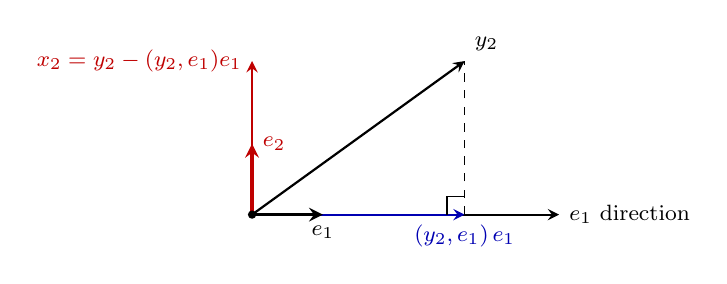
\begin{tikzpicture}[scale=1.5, >=stealth]
    \draw[->, thick] (0,0) -- (2.6,0) node[right] {$e_1$ direction};
    \draw[->, thick] (0,0) -- (1.8,1.3) node[above right] {$y_2$};
    \draw[->, thick, blue!70!black] (0,0) -- (1.8,0) node[below, blue!70!black] {$(y_2, e_1)\, e_1$};
    \draw[dashed] (1.8,0) -- (1.8,1.3);
    \draw (1.65,0) -- (1.65,0.15) -- (1.8,0.15);
    \draw[->, thick, red!75!black] (0,0) -- (0,1.3) node[left, red!75!black] {$x_2 = y_2 - (y_2, e_1) e_1$};
    \draw[->, very thick, red!75!black] (0,0) -- (0,0.6) node[right, red!75!black] {$e_2$};
    \draw[->, very thick] (0,0) -- (0.6,0) node[below] {$e_1$};
    \fill (0,0) circle (1pt);
\end{tikzpicture}
\end{center}
The step-by-step description looks countable, but it need not be: an orthonormal basis $\{e_\alpha\}_{\alpha \in \Lambda}$ need not be countable. The precise argument is Zorn's lemma, which says ``keep adding until nothing more can be added'' without any enumeration.
\end{rembox}

\begin{thmbox}[Existence of Orthonormal Bases]\boxlabel{thm:onbasis-exists}
Every Hilbert space $H$ has an orthonormal basis.
\laxref{\S6.4, Thm~9}
\end{thmbox}



\begin{proof}
If $H = \{0\}$, the empty set is an orthonormal basis: it is complete, since every $x \in H$ is $0$. Assume $H \neq \{0\}$.

\textbf{Step 1: the partially ordered set.} Let $S$ be the set of all orthonormal sets in $H$, partially ordered by inclusion: for $O_1, O_2 \in S$, $O_1 \prec O_2$ if $O_1 \subset O_2$. Two orthonormal sets need not be comparable. $S \neq \varnothing$: for any $x \neq 0$, $\{x/\|x\|\} \in S$.

\textbf{Step 2: every chain has an upper bound.} Let $C = \{O_\beta\}_{\beta \in I}$ be a chain in $S$ (if $C$ is empty, any element of $S$ is an upper bound), and let $U = \bigcup_{\beta \in I} O_\beta$. Then $U \in S$: each $u \in U$ lies in some $O_\beta$, so $\|u\| = 1$; and if $u \neq v$ in $U$, say $u \in O_{\beta_1}$ and $v \in O_{\beta_2}$, then since $C$ is a chain one of $O_{\beta_1}, O_{\beta_2}$ contains the other, so $u$ and $v$ lie in a single orthonormal set and $(u, v) = 0$. Since $O_\beta \subset U$ for every $\beta$, $U$ is an upper bound of $C$.

\textbf{Step 3: a maximal orthonormal set.} By Zorn's lemma (Theorem~\ref{thm:zorn}), $S$ has a maximal element $O = \{e_\alpha\}_{\alpha \in \Lambda}$.

\textbf{Step 4: $O$ is complete.} Suppose not. Then there is $x \in H$, $x \neq 0$, with $(x, e_\alpha) = 0$ for all $\alpha \in \Lambda$. Put $e = x/\|x\|$. Then $\|e\| = 1$ and $(e, e_\alpha) = 0$ for every $\alpha$; in particular $e \notin O$, since $(e, e) = 1 \neq 0$. So $O \cup \{e\}$ is an orthonormal set strictly containing $O$, contradicting the maximality of $O$. Hence $O$ is complete, and by Theorem~\ref{thm:onbasis-equiv} it is an orthonormal basis.
\end{proof}

\begin{defbox}[Separable Space]\boxlabel{def:separable}
A normed linear space $X$ is \textbf{separable} if it has a countable dense subset: a countable $D \subset X$ such that every $x \in X$ is a limit of a sequence in $D$. Completeness is not required.
\laxref{\S5.1, definition of separable space}
\end{defbox}

\subsubsection*{Examples of Separable and Non-Separable Spaces}

\begin{propbox}[{{$\ell^p$ is Separable for $1 \le p < \infty$}}]\boxlabel{prop:lp-separable}
Let $1 \le p < \infty$, and let $\mathbb{Q}_{\mathbb{F}} = \mathbb{Q}$ if $\mathbb{F} = \mathbb{R}$ and $\mathbb{Q}_{\mathbb{F}} = \mathbb{Q} + i\mathbb{Q}$ if $\mathbb{F} = \mathbb{C}$. The set
\[
D = \bigcup_{J = 1}^\infty \bigl\{ (p_1, \ldots, p_J, 0, 0, \ldots) : p_j \in \mathbb{Q}_{\mathbb{F}} \bigr\}
\]
is countable and dense in $\ell^p$. Hence $\ell^p$ is separable.
\end{propbox}

\begin{proof}
\emph{Countable.} For fixed $J$ the $J$-th set is in bijection with $\mathbb{Q}_{\mathbb{F}}^J$, a finite product of countable sets, hence countable; a countable union of countable sets is countable.

\emph{Dense.} Let $a = (a_j) \in \ell^p$ and $\varepsilon > 0$. Since $\sum_j |a_j|^p < \infty$, its tail is small: there is $J$ with $\sum_{j > J} |a_j|^p < (\varepsilon/2)^p$. Since $\mathbb{Q}_{\mathbb{F}}$ is dense in $\mathbb{F}$, choose $p_j \in \mathbb{Q}_{\mathbb{F}}$ with $|a_j - p_j| < \frac{\varepsilon}{2} J^{-1/p}$ for $j = 1, \ldots, J$, and let $d = (p_1, \ldots, p_J, 0, \ldots) \in D$. Then
\[
\|a - d\|_p^p = \sum_{j=1}^J |a_j - p_j|^p + \sum_{j > J} |a_j|^p < J \cdot \frac{(\varepsilon/2)^p}{J} + \Bigl(\frac{\varepsilon}{2}\Bigr)^p \le \varepsilon^p,
\]
so $\|a - d\|_p < \varepsilon$.
\end{proof}

\begin{center}
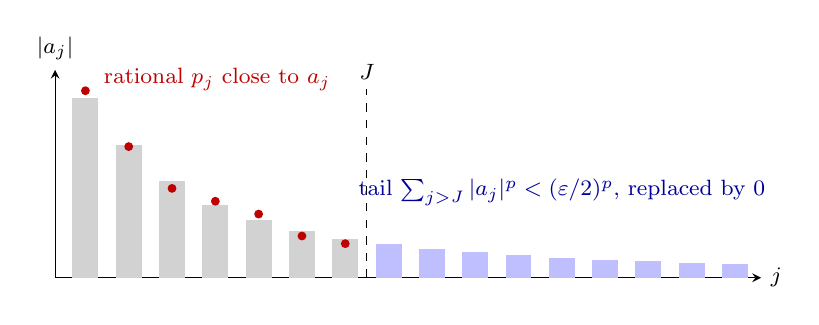
\begin{tikzpicture}[x=0.55cm, y=2.4cm, >=stealth]
    \draw[->] (0.3,0) -- (16.6,0) node[right] {$j$};
    \draw[->] (0.3,0) -- (0.3,1.1) node[above] {$|a_j|$};
    \foreach \j in {1,...,16} {
        \pgfmathsetmacro{\h}{0.95/(1+0.35*(\j-1)^1.3)}
        \ifnum\j<8
            \fill[gray!35] (\j-0.3,0) rectangle (\j+0.3,\h);
            \fill[red!75!black] (\j,{\h+0.04*sin(97*\j)}) circle (1.6pt);
        \else
            \fill[blue!25] (\j-0.3,0) rectangle (\j+0.3,\h);
        \fi
    }
    \draw[dashed] (7.5,0) -- (7.5,1.0) node[above] {$J$};
    \node[red!75!black, anchor=west] at (1.2,1.05) {rational $p_j$ close to $a_j$};
    \node[blue!60!black] at (12,0.45) {tail $\sum_{j > J} |a_j|^p < (\varepsilon/2)^p$, replaced by $0$};
\end{tikzpicture}
\end{center}
The two moves of the proof: cut off the tail, which is small because the series converges, and replace the finitely many remaining coordinates by nearby rationals. Both need $p < \infty$: the tail of a convergent series is small, but a bounded sequence need not have a small tail in the supremum norm.

\begin{propbox}[{{$\ell^\infty$ is Not Separable}}]\boxlabel{prop:linfty-nonsep}
$\ell^\infty$ is not separable.
\end{propbox}

\begin{proof}
Homework (HW5); to be added after submission.
\end{proof}

\begin{propbox}[{{$L^p(E)$ is Separable for $1 \le p < \infty$}}]\boxlabel{prop:Lp-separable}
Let $E \subset \mathbb{R}^n$ be measurable and $1 \le p < \infty$. Let $D$ be the set of functions on $E$ of the form
\[
\varphi = \sum_{j=1}^N a_j\, \chi_{R_j \cap E}, \qquad N \in \mathbb{N},\ a_j \in \mathbb{Q}_{\mathbb{F}},\ R_j \text{ a rectangle with rational endpoints},
\]
where a rectangle is a product $\prod_{i=1}^n [\alpha_i, \beta_i)$. Then $D$ is countable and dense in $L^p(E)$. Hence $L^p(E)$ is separable.
\end{propbox}

\begin{proof}
Wu's route: continuous functions are dense in $L^p$ (taken for granted), a continuous function is approximated by step functions, and the step functions can be taken with rational heights and rational rectangles. The details:

\emph{Countable.} A rectangle with rational endpoints is determined by $2n$ rationals, so there are countably many; for fixed $N$ the choices of $(a_1, \ldots, a_N, R_1, \ldots, R_N)$ form a finite product of countable sets; take the union over $N$.

\emph{Dense.} Let $f \in L^p(E)$ and $\varepsilon > 0$. Extend $f$ by $0$ to $\tilde{f}$ on $\mathbb{R}^n$; then $\tilde{f} \in L^p(\mathbb{R}^n)$ with the same norm.

\emph{Step 1: a continuous function.} By Theorem~\ref{thm:density} (with $\Omega = \mathbb{R}^n$) there is a continuous $g$ with compact support and $\|\tilde{f} - g\|_{L^p(\mathbb{R}^n)} < \varepsilon/3$. Choose $K \in \mathbb{N}$ with the support of $g$ inside $Q = [-K, K)^n$.

\emph{Step 2: a step function.} $g$ is uniformly continuous on the compact set $[-K,K]^n$. Let $\eta > 0$ with $\eta\,(2K)^{n/p} < \varepsilon/3$, and choose $\delta > 0$ with $|g(x) - g(y)| < \eta$ whenever $|x - y| < \delta$. Choose $m$ with $\sqrt{n}\,2^{-m} < \delta$ and partition $Q$ into the cubes $C_1, \ldots, C_M$ of the form $\prod_i [k_i 2^{-m}, (k_i + 1) 2^{-m})$, $k_i \in \mathbb{Z}$; they have rational endpoints. Let $c_k = g(z_k)$, $z_k$ the lower corner of $C_k$, and $\psi = \sum_k c_k \chi_{C_k}$. For $x \in C_k$, $|x - z_k| < \delta$, so $|g(x) - \psi(x)| < \eta$; outside $Q$ both vanish. Hence
\[
\|g - \psi\|_{L^p(\mathbb{R}^n)}^p = \int_Q |g - \psi|^p < \eta^p (2K)^n, \qquad \|g - \psi\|_{L^p(\mathbb{R}^n)} < \eta\,(2K)^{n/p} < \frac{\varepsilon}{3}.
\]

\emph{Step 3: rational heights.} Choose $q_k \in \mathbb{Q}_{\mathbb{F}}$ with $|c_k - q_k| < \eta$ and let $\tilde{\varphi} = \sum_k q_k \chi_{C_k}$. As in Step 2, $|\psi - \tilde{\varphi}| < \eta$ on $Q$ and $0$ outside, so $\|\psi - \tilde{\varphi}\|_{L^p(\mathbb{R}^n)} < \varepsilon/3$.

\emph{Step 4: restrict to $E$.} $\varphi = \tilde{\varphi}|_E = \sum_k q_k \chi_{C_k \cap E} \in D$, and since $\tilde{f} = f$ on $E$,
\[
\|f - \varphi\|_{L^p(E)} \le \|\tilde{f} - \tilde{\varphi}\|_{L^p(\mathbb{R}^n)} \le \|\tilde{f} - g\| + \|g - \psi\| + \|\psi - \tilde{\varphi}\| < \varepsilon. \qedhere
\]
\end{proof}

\begin{center}
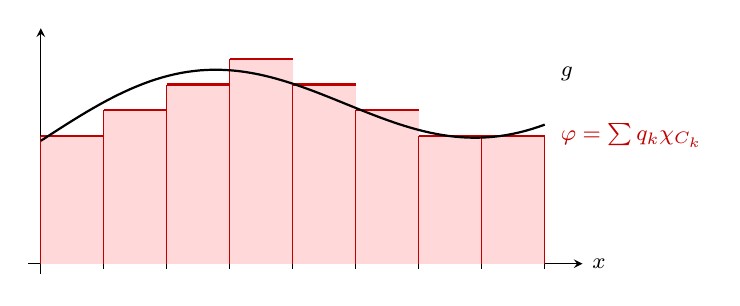
\begin{tikzpicture}[x=1.6cm, y=1.3cm, >=stealth]
    \draw[->] (-0.1,0) -- (4.3,0) node[right] {$x$};
    \draw[->] (0,-0.1) -- (0,2.3);
    \foreach \k in {0,...,7} {
        \pgfmathsetmacro{\xa}{0.5*\k}
        \pgfmathsetmacro{\c}{1.2+0.5*sin(deg(0.5*\k*1.3))+0.15*(0.5*\k)}
        \pgfmathsetmacro{\q}{round(\c*4)/4}
        \fill[red!15] (\xa,0) rectangle (\xa+0.5,\q);
        \draw[red!75!black, thick] (\xa,\q) -- (\xa+0.5,\q);
        \draw[red!75!black] (\xa,0) -- (\xa,\q);
    }
    \draw[red!75!black] (4,0) -- (4,{round((1.2+0.5*sin(deg(3.5*1.3))+0.15*3.5)*4)/4});
    \draw[thick, domain=0:4, samples=80] plot (\x, {1.2+0.5*sin(deg(\x*1.3))+0.15*\x});
    \node[anchor=west] at (4.05,1.85) {$g$};
    \node[red!75!black, anchor=west] at (4.05,1.25) {$\varphi = \sum q_k \chi_{C_k}$};
    \foreach \x in {0,0.5,...,4} \draw (\x,0) -- (\x,-0.05);
\end{tikzpicture}
\end{center}
A continuous $g$ and a step function on cubes with rational endpoints and rational heights (here $n = 1$, heights rounded to quarters). The $L^p$ distance is small because it is an \emph{integral} of a small difference over a bounded set. In $L^\infty$ the distance is a supremum, and this argument breaks down.

\begin{propbox}[{{$L^\infty(E)$ is Not Separable}}]\boxlabel{prop:Linfty-nonsep}
If $E \subset \mathbb{R}^n$ is measurable with $m(E) > 0$, then $L^\infty(E)$ is not separable.
\end{propbox}

\begin{proof}
Stated in lecture without proof; the argument is close to the homework on $\ell^\infty$ (Proposition~\ref{prop:linfty-nonsep}) and will be added after that is submitted.
\end{proof}

\begin{rembox}\label{rem:onb-7}
The hypothesis $m(E) > 0$ is added here: if $m(E) = 0$, then $L^\infty(E) = \{0\}$, which is separable. Wu stressed that measure theory supplies the examples of functional analysis (``I would suggest you really study real methods \ldots\ measure theory is becoming very useful now''): without $L^p$ the course has few examples beyond sequence spaces.
\end{rembox}

\subsubsection*{Countable Orthonormal Bases}

\begin{thmbox}[Separable Hilbert Spaces and Countable Bases]\boxlabel{thm:sep-countable-onb}
A Hilbert space $H$ has a countable orthonormal basis if and only if it is separable.
\laxref{\S6.4, Thm~9$'$}
\end{thmbox}

\begin{proof}[Proof of ($\Rightarrow$)]
Assume $H$ has a countable orthonormal basis $\{e_1, e_2, \ldots\}$ (finite or infinite). Then $H = \overline{\operatorname{span}}\{e_1, e_2, \ldots\}$: every $x \in H$ is $x = \sum_j (x, e_j)\, e_j$ (Theorem~\ref{thm:onbasis-equiv}), a finite sum if the basis is finite and a limit of partial sums otherwise. Let
\[
D = \bigcup_{n} \Bigl\{ \sum_{j=1}^n a_j e_j : a_j \in \mathbb{Q}_{\mathbb{F}} \Bigr\},
\]
the union over $n = 1, 2, \ldots$ (only up to the number of basis vectors if the basis is finite). Each set in the union is in bijection with $\mathbb{Q}_{\mathbb{F}}^n$, so $D$ is countable.

\emph{$D$ is dense.} Let $x \in H$ and $\varepsilon > 0$. The partial sums of the expansion converge to $x$, so there is $n$ with $\bigl\| x - \sum_{j=1}^n (x, e_j) e_j \bigr\| < \varepsilon/2$ (if the basis is finite, take $n$ its size, and this term is $0$). Choose $a_j \in \mathbb{Q}_{\mathbb{F}}$ with $|(x, e_j) - a_j| < \frac{\varepsilon}{2\sqrt{n}}$. By Pythagoras (Lemma~\ref{lem:pythagoras}),
\[
\Bigl\| \sum_{j=1}^n \bigl( (x, e_j) - a_j \bigr) e_j \Bigr\|^2 = \sum_{j=1}^n |(x, e_j) - a_j|^2 < n \cdot \frac{\varepsilon^2}{4n} = \frac{\varepsilon^2}{4},
\]
so $\bigl\| x - \sum_{j=1}^n a_j e_j \bigr\| < \varepsilon/2 + \varepsilon/2 = \varepsilon$. The tail of the expansion is small, as for $\ell^p$.
\end{proof}

For the converse, the countable dense set has to be turned into an orthonormal set, which is the Gram--Schmidt process.

\begin{lembox}[Gram--Schmidt]\boxlabel{lem:gram-schmidt}
Let $y_1, y_2, \ldots$ be a finite or infinite sequence of linearly independent vectors in an inner product space $X$. Then there is an orthonormal sequence $e_1, e_2, \ldots$ (of the same length) with
\[
\operatorname{span}\{y_1, \ldots, y_j\} = \operatorname{span}\{e_1, \ldots, e_j\} \qquad \text{for every } j.
\]
\laxref{\S6.4, Thm~9$'$}
\end{lembox}

\begin{proof}
Define recursively
\[
e_1 = \frac{y_1}{\|y_1\|}, \qquad x_j = y_j - \sum_{i=1}^{j-1} (y_j, e_i)\, e_i, \qquad e_j = \frac{x_j}{\|x_j\|} \quad (j \ge 2),
\]
exactly as in the informal construction in the remark before Theorem~\ref{thm:onbasis-exists}: subtract from $y_j$ its components along the directions already built, and normalize. We check by induction on $j$ that the recursion is well defined and that $\{e_1, \ldots, e_j\}$ is orthonormal with $\operatorname{span}\{e_1, \ldots, e_j\} = \operatorname{span}\{y_1, \ldots, y_j\}$.

\emph{$j = 1$.} $y_1 \neq 0$ by linear independence, so $e_1$ is defined, $\|e_1\| = 1$, and $\operatorname{span}\{e_1\} = \operatorname{span}\{y_1\}$.

\emph{From $j - 1$ to $j$.} \emph{$x_j \neq 0$:} otherwise $y_j = \sum_{i<j} (y_j, e_i) e_i \in \operatorname{span}\{e_1, \ldots, e_{j-1}\} = \operatorname{span}\{y_1, \ldots, y_{j-1}\}$, contradicting linear independence. So $e_j$ is defined and $\|e_j\| = 1$. \emph{Orthogonality:} for $k < j$, using $(e_i, e_k) = \delta_{ik}$ for $i, k < j$,
\[
(x_j, e_k) = (y_j, e_k) - \sum_{i=1}^{j-1} (y_j, e_i)(e_i, e_k) = (y_j, e_k) - (y_j, e_k) = 0,
\]
so $(e_j, e_k) = 0$. \emph{Spans:} $e_j$ is a combination of $y_j$ and $e_1, \ldots, e_{j-1} \in \operatorname{span}\{y_1, \ldots, y_{j-1}\}$, so $e_j \in \operatorname{span}\{y_1, \ldots, y_j\}$; conversely $y_j = \|x_j\|\, e_j + \sum_{i<j} (y_j, e_i) e_i \in \operatorname{span}\{e_1, \ldots, e_j\}$. With the induction hypothesis, the two spans are equal.

Since $e_j$ depends only on $y_1, \ldots, y_j$, the recursion runs through an infinite sequence as well.
\end{proof}

\begin{proof}[Proof of ($\Leftarrow$) in Theorem~\ref{thm:sep-countable-onb}]
Assume $D = \{y_1, y_2, \ldots\}$ is a countable dense subset of $H$. If $H = \{0\}$, the empty set is a countable orthonormal basis; assume $H \neq \{0\}$, so $D$ contains a nonzero element.

\textbf{Step 1: a linearly independent subsequence.} Discard elements that depend linearly on earlier ones. Precisely: let $n_1$ be the first index with $y_{n_1} \neq 0$, and put $y_1' = y_{n_1}$. Having chosen $n_1 < \cdots < n_k$, let $n_{k+1}$ be the first index $n > n_k$ with $y_n \notin \operatorname{span}\{y_1', \ldots, y_k'\}$, and put $y_{k+1}' = y_{n_{k+1}}$; if there is no such index, stop. Wu: ``we just take the first linearly independent one, name it $y_2'$, then continue.'' The result $D' = \{y_1', y_2', \ldots\}$ (finite or infinite) is linearly independent by construction, and every element of $D$ is a linear combination of elements of $D'$: an element $y_j$ that was discarded, with $n_k < j < n_{k+1}$ (or $j > n_k$ if the process stopped at $k$), lies in $\operatorname{span}\{y_1', \ldots, y_k'\}$, and $y_j = 0$ if $j < n_1$. So
\begin{equation}\label{eq:gs-span}
\text{for every } y_j \in D \text{ there is } k \text{ with } y_j \in \operatorname{span}\{y_1', \ldots, y_k'\}.
\end{equation}

\textbf{Step 2: Gram--Schmidt.} Lemma~\ref{lem:gram-schmidt} gives an orthonormal sequence $\{e_1, e_2, \ldots\}$ with
\[
\operatorname{span}\{e_1, \ldots, e_j\} = \operatorname{span}\{y_1', \ldots, y_j'\} \qquad \text{for every } j.
\] It is countable; it remains to show it is complete, hence (Theorem~\ref{thm:onbasis-equiv}) an orthonormal basis.

\textbf{Step 3: completeness.} Let $x \in H$ with $(x, e_j) = 0$ for all $j$; we show $x = 0$. Since $D$ is dense in $H$, there is a sequence $y_{n_k} \in D$ with $\lim_{k \to \infty} y_{n_k} = x$. By \eqref{eq:gs-span} and Step 2, each $y_{n_k}$ lies in $\operatorname{span}\{e_1, \ldots, e_{j_k}\}$ for some $j_k$, say $y_{n_k} = \sum_{j=1}^{j_k} a_j^{(k)} e_j$. Then
\[
(x, y_{n_k}) = \sum_{j=1}^{j_k} \overline{a_j^{(k)}}\, (x, e_j) = 0 \qquad \text{for all } k,
\]
and by continuity of the inner product (Lemma~\ref{lem:ip-continuous}),
\[
(x, x) = \lim_{k \to \infty} (x, y_{n_k}) = 0 .
\]
Hence $x = 0$, and $\{e_j\}$ is complete.
\end{proof}

\begin{rembox}\label{rem:onb-8}
The dense set $D$ is used twice, for different purposes: its span supplies the orthonormal vectors, and its density supplies the approximating sequence in Step~3. Only finite linear combinations appear anywhere --- the limit is taken in the inner product, not in the expansion. Compare Proposition~\ref{prop:sep-countable}: in a separable Hilbert space \emph{every} orthonormal set is countable, not just the one constructed here.
\end{rembox}

\subsubsection*{Classification of Separable Hilbert Spaces}

\begin{defbox}[Isomorphic Hilbert Spaces]\boxlabel{def:hilbert-iso}
Let $H_1$ and $H_2$ be Hilbert spaces over the same field, with inner products $(\cdot, \cdot)_1$ and $(\cdot, \cdot)_2$. $H_1$ is \textbf{isomorphic} to $H_2$ if there is a map $T : H_1 \to H_2$ that is linear, one-to-one and onto, and preserves the inner product:
\[
(Tx, Ty)_2 = (x, y)_1 \qquad \text{for all } x, y \in H_1 .
\]
\end{defbox}

\begin{rembox}[Isomorphic or Isometric?]\label{rem:isomorphic-or-isometric}
A student asked whether ``isomorphic'' here means the map preserves distance. It does: $\|Tx - Ty\|_2^2 = (T(x-y), T(x-y))_2 = \|x - y\|_1^2$, so $T$ is an \emph{isometry}. Preserving the inner product already forces one-to-one ($Tx = 0$ gives $\|x\|_1 = \|Tx\|_2 = 0$). What it does not force is \emph{onto}, which is why the definition requires a bijection; the next example shows the difference. (The example is not from lecture.)
\end{rembox}

\begin{exbox}[An Isometry That is Not an Isomorphism]\boxlabel{ex:isometry-not-isomorphism}
On $\ell^2$ let $S(a_1, a_2, \ldots) = (0, a_1, a_2, \ldots)$. $S$ is linear and $(Sa, Sb) = \sum_{j \ge 1} a_j \overline{b_j} = (a, b)$, so $S$ preserves the inner product. It is not onto: every $Sa$ has first coordinate $0$, so $e_1 = (1, 0, 0, \ldots)$ is not in the range.
\end{exbox}

\begin{thmbox}[Classification of Separable Hilbert Spaces]\boxlabel{thm:sep-classification}
Every separable Hilbert space $H$ over $\mathbb{F}$ is isomorphic either to $\mathbb{F}^n$ for some $n \in \{0, 1, 2, \ldots\}$, or to $\ell^2$.
\laxref{\S6.4, Exercise~10}
\end{thmbox}

\begin{proof}
Homework (HW5); to be added after submission.
\end{proof}

\begin{rembox}\label{rem:onb-9}
On the board: ``isomorphic either to $\mathbb{R}^n$, $n \in \mathbb{N}$, or $\ell^2$'' --- the real case. Over $\mathbb{C}$ the finite-dimensional models are $\mathbb{C}^n$, and $n = 0$ covers $H = \{0\}$. By Theorem~\ref{thm:sep-countable-onb} a separable $H$ has a countable orthonormal basis; the finite case gives $\mathbb{F}^n$ and the infinite case $\ell^2$.
\end{rembox}

% ============================================================================
% CHAPTER 6: BOUNDED LINEAR MAPS
% ============================================================================

\chapter{Bounded Linear Maps}\label{ch:maps}

Linear functionals take values in the scalars. The next objects are linear maps between two normed linear spaces, and the question is the same as for functionals: when is a linear map continuous, and how large is it? The answer --- continuity and boundedness coincide, and the bounded maps form a normed space of their own, complete when the target is --- is the starting point for operators on Hilbert space. The material follows Lax, Chapter 15.

% Lecture 9 (2026-09-29), last part

\section{Boundedness and Continuity}\label{sec:bounded-maps}

\roadmark{Stage: maps}{Thread: functionals. Linear functionals generalize to linear maps between normed spaces; the bounded functionals of \ref{sec:riesz-rep} are the case $Y = \mathbb{F}$.}

Throughout, $(X, \|\cdot\|_X)$ and $(Y, \|\cdot\|_Y)$ are normed linear spaces over the same field $\mathbb{F}$; neither needs to be complete (``no completeness is necessary'' for continuity, since only sequences that already converge are involved).

\begin{defbox}[Continuous Linear Map]\boxlabel{def:cont-map}
A map $T : X \to Y$ is \textbf{linear} if $T(a_1 x_1 + a_2 x_2) = a_1 T x_1 + a_2 T x_2$ for all $x_1, x_2 \in X$ and $a_1, a_2 \in \mathbb{F}$. It is \textbf{continuous} if for every sequence $\{x_j\}_{j \in \mathbb{N}}$ in $X$,
\[
x_j \to x^{(0)} \text{ in } (X, \|\cdot\|_X) \implies T x_j \to T x^{(0)} \text{ in } (Y, \|\cdot\|_Y).
\]
\laxref{\S15.1, definition of continuous map}
\end{defbox}

\begin{defbox}[Bounded Linear Map; Operator Norm]\boxlabel{def:bounded-map}
A linear map $T : X \to Y$ is \textbf{bounded} if there is $M \ge 0$ with
\[
\|T x\|_Y \le M\, \|x\|_X \qquad \text{for all } x \in X .
\]
For a bounded $T$ (and $X \neq \{0\}$) its \textbf{norm} is
\[
\|T\| = \sup_{\substack{x \in X \\ x \neq 0}} \frac{\|T x\|_Y}{\|x\|_X} ;
\]
if $X = \{0\}$, put $\|T\| = 0$.
\laxref{\S15.1, (2) and (2$'$)}
\end{defbox}

\begin{propbox}[The Operator Norm]\boxlabel{prop:op-norm}
Let $T : X \to Y$ be a bounded linear map, $X \neq \{0\}$. Then
\begin{enumerate}[label=(\alph*)]
    \item $\|T\| = \sup_{\|x\|_X = 1} \|T x\|_Y$;
    \item $\|T x\|_Y \le \|T\|\, \|x\|_X$ for all $x \in X$;
    \item $\|T\|$ is the smallest $M$ for which $\|Tx\|_Y \le M \|x\|_X$ holds for all $x$.
\end{enumerate}
\laxref{\S15.1, (3) and (3$'$)}
\end{propbox}

\begin{proof}
(Stated in lecture; the checks are written out here.) (a) For $x \neq 0$, $u = x/\|x\|_X$ has $\|u\|_X = 1$ and, by linearity and homogeneity, $\|T x\|_Y / \|x\|_X = \|T u\|_Y$. So the ratios over $x \neq 0$ and the values $\|Tu\|_Y$ over unit vectors $u$ form the same set of numbers, and the two suprema agree. Both are finite: if $\|Tx\|_Y \le M\|x\|_X$ for all $x$, every ratio is at most $M$.

(b) For $x = 0$ both sides are $0$, since $T0 = 0$ by linearity. For $x \neq 0$, $\|Tx\|_Y / \|x\|_X \le \|T\|$ by definition of the supremum.

(c) By (b), $M = \|T\|$ works. If $M$ works, every ratio is at most $M$, so $\|T\| \le M$.
\end{proof}

\begin{propbox}[Continuous if and only if Bounded]\boxlabel{prop:cont-bounded}
A linear map $T : X \to Y$ between normed linear spaces is continuous if and only if it is bounded.
\laxref{\S15.1, Thm~1}
\end{propbox}

\begin{proof}
($\Leftarrow$, the easy direction.) Let $\|Tx\|_Y \le M \|x\|_X$ for all $x$, and let $x_j \to x^{(0)}$. By linearity,
\[
\|T x_j - T x^{(0)}\|_Y = \|T(x_j - x^{(0)})\|_Y \le M\, \|x_j - x^{(0)}\|_X \to 0 .
\]

($\Rightarrow$) Assume $T$ is continuous but not bounded. Then no $M$ works; in particular, for each $n \in \mathbb{N}$ the constant $M = n$ fails, so there is $x_n \in X$ with
\[
\|T x_n\|_Y > n\, \|x_n\|_X ,
\]
and $x_n \neq 0$, since for $x_n = 0$ both sides would be $0$. Let
\[
y_n = \frac{x_n}{n\, \|x_n\|_X} .
\]
Then $\|y_n\|_X = \frac{1}{n} \to 0$, so $y_n \to 0$ in $X$. By linearity $T y_n = \frac{1}{n \|x_n\|_X}\, T x_n$, so
\[
\|T y_n\|_Y = \frac{\|T x_n\|_Y}{n\, \|x_n\|_X} > 1 \qquad \text{for all } n .
\]
But $T 0 = 0$, so continuity would give $\|T y_n\|_Y = \|T y_n - T0\|_Y \to 0$. This contradicts $\|T y_n\|_Y > 1$. Hence $T$ is bounded.
\end{proof}

\begin{center}
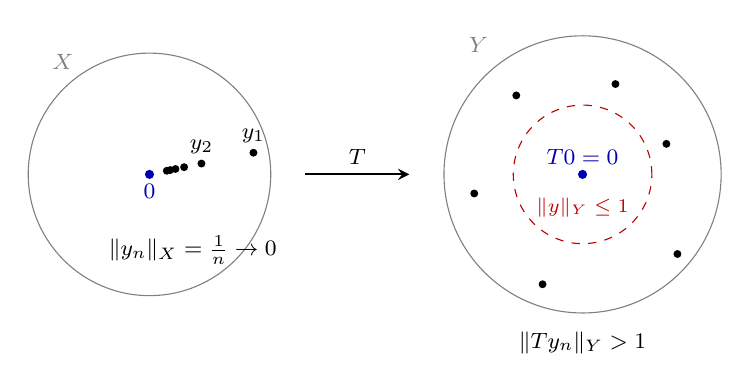
\begin{tikzpicture}[scale=1.1, >=stealth]
    \begin{scope}
        \draw[gray] (0,0) circle (1.4);
        \node[gray] at (-1.0,1.3) {$X$};
        \foreach \n in {1,...,6} {\fill (1.2/\n,0.25/\n) circle (1.3pt);}
        \node[above] at (1.2,0.25) {$y_1$};
        \node[above] at (0.6,0.125) {$y_2$};
        \fill[blue!70!black] (0,0) circle (1.5pt) node[below, blue!70!black] {$0$};
        \node[below] at (0.5,-0.6) {$\|y_n\|_X = \tfrac1n \to 0$};
    \end{scope}
    \draw[->, thick] (1.8,0) -- (3.0,0) node[midway, above] {$T$};
    \begin{scope}[xshift=5cm]
        \draw[gray] (0,0) circle (1.6);
        \node[gray] at (-1.2,1.5) {$Y$};
        \draw[dashed, red!75!black] (0,0) circle (0.8);
        \node[red!75!black, font=\scriptsize] at (0,-0.38) {$\|y\|_Y \le 1$};
        \foreach \n/\a in {1/20,2/70,3/130,4/190,5/250,6/320} {\fill ({(0.95+0.08*\n)*cos(\a)},{(0.95+0.08*\n)*sin(\a)}) circle (1.3pt);}
        \fill[blue!70!black] (0,0) circle (1.5pt) node[above, blue!70!black] {$T0 = 0$};
        \node[below] at (0,-1.7) {$\|T y_n\|_Y > 1$};
    \end{scope}
\end{tikzpicture}
\end{center}
The proof of ($\Rightarrow$): an unbounded $T$ sends the sequence $y_n \to 0$ to points that all stay outside the unit ball, so $Ty_n \not\to T0$.

\begin{rembox}\label{rem:bounded-maps}
For $Y = \mathbb{F}$ this is Proposition~\ref{prop:bounded-continuous} on linear functionals, and $\|T\|$ is then the dual norm of Definition~\ref{def:dual-space}. The companion chapter's bounded operators on $H$ (Definition~\ref{def:operator}) are the case $X = Y = H$. Since $\|Tx - Tx'\|_Y \le \|T\|\, \|x - x'\|_X$, a bounded linear map is even Lipschitz continuous, uniformly on all of $X$.
\end{rembox}

% Lecture 10 (2026-10-01)

\subsection{Examples}

Wu opened Lecture 10 with examples: ``in reality we actually need to work on linear maps because nonlinear ones are very difficult.'' Whether a map is bounded depends on the norms, not only on the formula.

\begin{exbox}[Differentiation is Bounded from $C^m$ to $C^{m-1}$]\boxlabel{ex:diff-bounded}
Let $\Omega \subset \mathbb{R}^n$ be bounded and open, and let $C^m(\overline{\Omega})$ be the functions on $\Omega$ whose partial derivatives $\partial^\alpha f$ of all orders $|\alpha| \le m$ exist, are continuous, and extend continuously to the compact set $\overline{\Omega}$, with the norm
\[
\|f\|_{C^m(\overline{\Omega})} = \sum_{|\alpha| \le m} \|\partial^\alpha f\|_{L^\infty(\Omega)}, \qquad \|g\|_{L^\infty(\Omega)} = \max_{x \in \overline{\Omega}} |g(x)| .
\]
For $m \ge 1$, $Tf = \partial_{x_1} f$ is a linear map $C^m(\overline{\Omega}) \to C^{m-1}(\overline{\Omega})$, and it is bounded with $\|T\| \le 1$:
\[
\|Tf\|_{C^{m-1}(\overline{\Omega})} \le \|f\|_{C^m(\overline{\Omega})} \qquad \text{for all } f \in C^m(\overline{\Omega}).
\]
\end{exbox}

\begin{proof}
%% FILL-IN: Wu stated the bound; the counting of derivatives is written out here.
Linearity is linearity of differentiation. For a multi-index $\beta$ with $|\beta| \le m - 1$, $\partial^\beta(\partial_{x_1} f) = \partial^{\beta + e_1} f$, where $\beta + e_1$ has order $|\beta| + 1 \le m$, and distinct $\beta$ give distinct $\beta + e_1$. So the terms of
\[
\|Tf\|_{C^{m-1}} = \sum_{|\beta| \le m-1} \|\partial^{\beta + e_1} f\|_{L^\infty}
\]
are some of the terms of $\|f\|_{C^m} = \sum_{|\alpha| \le m} \|\partial^\alpha f\|_{L^\infty}$, all non-negative, and the inequality follows.
\end{proof}

\begin{rembox}\label{rem:bounded-maps-2}
Wu noted that $C^m(\overline{\Omega})$ is complete in this norm and left that to the class; it is not needed for the example. For $m = 1$ and $\Omega = (a,b)$ it is Part~2 of the proof of Proposition~\ref{prop:C2-incomplete}.
\end{rembox}

\begin{propbox}[{{Differentiation is Unbounded in the Maximum Norm}}]\boxlabel{prop:diff-unbounded}
Give $C^\infty(\overline{\Omega})$ the norm $\|f\| = \max_{x \in \overline{\Omega}} |f(x)|$ (a norm under which $C^\infty(\overline{\Omega})$ is not complete). Then $Tf = \partial_{x_1} f$ is a linear map $C^\infty(\overline{\Omega}) \to C^\infty(\overline{\Omega})$ that is \emph{not} bounded: there is no $M$ with $\max_{\overline{\Omega}} |\partial_{x_1} f| \le M \max_{\overline{\Omega}} |f|$ for all $f$.
\end{propbox}

\begin{proof}
Homework; to be added after submission.
\end{proof}

%% >>> ADDED: remark (Claude commentary)
\begin{rembox}\label{rem:bounded-maps-3}
The two examples have the same formula and opposite answers. In the first, the norm of the target counts one derivative fewer than the norm of the domain, so the derivative taken by $T$ is already paid for; in the second, both norms see only the values of $f$, and ``you cannot control derivatives by functions.''
\end{rembox}
%% <<< END ADDED

\begin{exbox}[The Fourier Transform from $L^1$ to $L^\infty$]\boxlabel{ex:fourier-L1}
For $f \in L^1(\mathbb{R}^n)$ define
\[
\mathcal{F}(f)(x) = \int_{\mathbb{R}^n} e^{-i x \cdot \xi} f(\xi)\, d\xi, \qquad x \cdot \xi = \sum_{j=1}^n x_j \xi_j .
\]
Then $\mathcal{F} : L^1(\mathbb{R}^n) \to L^\infty(\mathbb{R}^n)$ is a bounded linear map with
\[
\|\mathcal{F}(f)\|_{L^\infty(\mathbb{R}^n)} \le \|f\|_{L^1(\mathbb{R}^n)} .
\]
\laxref{\S16.1, Thm~1(i); \S16.3.1}
\end{exbox}

\begin{proof}
For fixed $x$, $|e^{-ix\cdot\xi} f(\xi)| = |f(\xi)|$ since $|e^{-ix\cdot\xi}| = 1$, so the integrand is integrable and
\[
|\mathcal{F}(f)(x)| \le \int_{\mathbb{R}^n} |f(\xi)|\, d\xi = \|f\|_{L^1}
\]
for every $x$. %% FILL-IN: the points below are not from the board.
Changing $f$ on a null set does not change the integral, so $\mathcal{F}$ is defined on classes, and it is linear by linearity of the integral. $\mathcal{F}(f)$ is measurable (in fact continuous: if $x_k \to x$, the integrands converge pointwise and are dominated by $|f|$, so the dominated convergence theorem gives $\mathcal{F}(f)(x_k) \to \mathcal{F}(f)(x)$). Hence $\mathcal{F}(f) \in L^\infty$ with $\|\mathcal{F}(f)\|_{L^\infty} \le \|f\|_{L^1}$.
\end{proof}

\begin{propbox}[Linear Maps on Finite-Dimensional Spaces are Bounded]\boxlabel{prop:findim-bounded}
Let $X$ and $Y$ be normed linear spaces with $\dim X < \infty$. Every linear map $T : X \to Y$ is bounded.
\end{propbox}

\begin{proof}
%% FILL-IN: Wu left this to the class ("you can figure out by yourself"); the proof is written out here.
(Left to the class in lecture.) Let $e_1, \ldots, e_n$ be a basis of $X$ and $\|x\|_1 = \sum_i |a_i|$ for $x = \sum_i a_i e_i$ (Step~2 of the proof of Theorem~\ref{prop:norms-equiv}). By linearity and the triangle inequality,
\[
\|Tx\|_Y = \Bigl\| \sum_i a_i\, T e_i \Bigr\|_Y \le \sum_i |a_i|\, \|T e_i\|_Y \le \Bigl( \max_i \|T e_i\|_Y \Bigr) \|x\|_1 .
\]
By Theorem~\ref{prop:norms-equiv}, $\|x\|_1 \le C\|x\|_X$ for some $C$, so $\|Tx\|_Y \le C \max_i \|Te_i\|_Y\, \|x\|_X$.
\end{proof}

\begin{defbox}[{{The Space $\mathcal{L}(X, Y)$}}]\boxlabel{def:LXY}
$\mathcal{L}(X, Y)$ is the set of all bounded linear maps $T : X \to Y$, with the pointwise operations $(T_1 + T_2)x = T_1 x + T_2 x$ and $(aT)x = a\, Tx$, and the norm $\|T\|$ of Definition~\ref{def:bounded-map}.
\laxref{\S15.1, definition of $\mathcal{L}(X, U)$}
\end{defbox}

\begin{thmbox}[{{$\mathcal{L}(X, Y)$ is a Normed Linear Space}}]\boxlabel{thm:LXY}
Let $X$ and $Y$ be normed linear spaces.
\begin{enumerate}[label=(\arabic*)]
    \item $(\mathcal{L}(X, Y), \|\cdot\|)$ is a normed linear space.
    \item If $Y$ is complete, then $\mathcal{L}(X, Y)$ is a Banach space.
\end{enumerate}
\laxref{\S15.1, Thms~2--3}
\end{thmbox}

\begin{proof}[Proof of (1)]
We may assume $X \neq \{0\}$; otherwise $\mathcal{L}(X, Y) = \{0\}$.

\emph{Linear space.} The set of all maps $X \to Y$ with pointwise operations is a linear space: each of the eight axioms, evaluated at a point $x \in X$, is the corresponding axiom of $Y$ (as in Part~1 of the proof of Theorem~\ref{thm:Cab-banach}, with $\mathbb{F}$ replaced by $Y$). $\mathcal{L}(X, Y)$ is a linear subspace of it. The zero map is linear and bounded with $M = 0$. If $T_1, T_2$ are linear, so are $T_1 + T_2$ and $aT_1$: $(T_1 + T_2)(a_1 x_1 + a_2 x_2) = a_1 T_1 x_1 + a_2 T_1 x_2 + a_1 T_2 x_1 + a_2 T_2 x_2 = a_1 (T_1 + T_2) x_1 + a_2 (T_1 + T_2) x_2$, and similarly for $aT_1$. If $\|T_i x\|_Y \le M_i \|x\|_X$, then $\|(T_1 + T_2)x\|_Y \le \|T_1 x\|_Y + \|T_2 x\|_Y \le (M_1 + M_2)\|x\|_X$ and $\|(aT_1)x\|_Y = |a|\,\|T_1 x\|_Y \le |a| M_1 \|x\|_X$.

\emph{Positivity.} $\|T\| \ge 0$ as a supremum of non-negative numbers. If $\|T\| = 0$, then by Proposition~\ref{prop:op-norm}(b), $\|Tx\|_Y \le 0$ for all $x$, so $Tx = 0$ for all $x$ and $T$ is the zero map; conversely the zero map has norm $0$.

\emph{Homogeneity.} (Left to us in lecture.) By Proposition~\ref{prop:op-norm}(a), $\|aT\| = \sup_{\|x\|_X = 1} \|a\, Tx\|_Y = \sup_{\|x\|_X = 1} |a|\,\|Tx\|_Y = |a| \sup_{\|x\|_X = 1} \|Tx\|_Y = |a|\,\|T\|$, since multiplying a set of non-negative numbers by $|a| \ge 0$ multiplies its supremum by $|a|$.

\emph{Subadditivity.} By Proposition~\ref{prop:op-norm}(a),
\begin{align*}
\|T_1 + T_2\| &= \sup_{\|x\|_X = 1} \|T_1 x + T_2 x\|_Y \le \sup_{\|x\|_X = 1} \bigl( \|T_1 x\|_Y + \|T_2 x\|_Y \bigr) \\
&\le \sup_{\|x\|_X = 1} \|T_1 x\|_Y + \sup_{\|x\|_X = 1} \|T_2 x\|_Y = \|T_1\| + \|T_2\| .
\end{align*}
The first inequality is the triangle inequality in $Y$ at each $x$. The second holds because for every unit $x$, $\|T_1 x\|_Y + \|T_2 x\|_Y \le \|T_1\| + \|T_2\|$, so the right-hand side is an upper bound for the set whose supremum is taken: summing and then taking the supremum gives at most the sum of the separate suprema.
\end{proof}

\begin{proof}[Proof of (2)]
(Lecture 10.) Assume $Y$ is complete, and let $\{T_n\}$ be a Cauchy sequence in $\mathcal{L}(X, Y)$: for every $\varepsilon > 0$ there is $N$ with $\|T_n - T_k\| < \varepsilon$ for all $n, k \ge N$.

\textbf{Step 1: pointwise limits.} Fix $x_0 \in X$. By Proposition~\ref{prop:op-norm}(b),
\[
\|T_n x_0 - T_k x_0\|_Y = \|(T_n - T_k) x_0\|_Y \le \|T_n - T_k\|\, \|x_0\|_X \le \varepsilon\, \|x_0\|_X \qquad (n, k \ge N),
\]
so $\{T_n x_0\}$ is a Cauchy sequence in $Y$. Since $Y$ is complete, it converges. Define
\[
T x_0 = \lim_{n \to \infty} T_n x_0 \qquad (x_0 \in X).
\]
This is the candidate.

\textbf{Step 2: $T$ is linear.} For $a_1, a_2 \in \mathbb{F}$ and $x_1, x_2 \in X$, $T_n(a_1 x_1 + a_2 x_2) = a_1 T_n x_1 + a_2 T_n x_2$. As $n \to \infty$ the left side converges to $T(a_1 x_1 + a_2 x_2)$ and the right side to $a_1 T x_1 + a_2 T x_2$ %% FILL-IN: why the right side converges.
(since $\|(a_1 T_n x_1 + a_2 T_n x_2) - (a_1 T x_1 + a_2 T x_2)\|_Y \le |a_1|\,\|T_n x_1 - T x_1\|_Y + |a_2|\,\|T_n x_2 - T x_2\|_Y \to 0$). Limits are unique, so $T(a_1 x_1 + a_2 x_2) = a_1 T x_1 + a_2 T x_2$.

\textbf{Step 3: the uniform estimate.} Let $\varepsilon > 0$ and $N$ as above. For every $x \in X$ and $n, k \ge N$, $\|T_n x - T_k x\|_Y \le \varepsilon\,\|x\|_X$. Fix $x$ and $k \ge N$. For any $n \ge N$, by the triangle inequality,
\[
\|T x - T_k x\|_Y \le \|T x - T_n x\|_Y + \|T_n x - T_k x\|_Y \le \|T_n x - T x\|_Y + \varepsilon\, \|x\|_X .
\]
The left side does not depend on $n$; letting $n \to \infty$, the first term on the right tends to $0$ by Step 1, so
\[
\|T_k x - T x\|_Y \le \varepsilon\, \|x\|_X \qquad \text{for all } x \in X \text{ and all } k \ge N .
\]

\textbf{Step 4: conclusion.} By Step 2, $T_k - T$ is linear, and by Step 3 it is bounded with $\|T_k - T\| \le \varepsilon$ for $k \ge N$. Since $\mathcal{L}(X, Y)$ is a linear space (part (1)) and $T_k, T_k - T \in \mathcal{L}(X, Y)$, also $T = T_k - (T_k - T) \in \mathcal{L}(X, Y)$. Finally $\|T_k - T\| \le \varepsilon$ for all $k \ge N$ says $T_k \to T$ in $\mathcal{L}(X, Y)$. So every Cauchy sequence converges, and $\mathcal{L}(X, Y)$ is a Banach space.
\end{proof}

\begin{rembox}[Why $\varepsilon$ Does Not Depend on $x$]\label{rem:why-does-not-depend-x}
A student asked whether $\varepsilon$ in Step 3 varies with $x$. It does not: $N$ is chosen from $\|T_n - T_k\| < \varepsilon$ alone, and $\|T_n - T_k\|$ is the supremum of $\|T_n x - T_k x\|_Y/\|x\|_X$ over all $x$, so the single inequality $\|T_n x - T_k x\|_Y \le \varepsilon\|x\|_X$ holds for every $x$ at once. That is what makes $\|T_k - T\| \le \varepsilon$ legitimate at the end. If $N$ depended on $x$, the conclusion would only be pointwise convergence. Wu compared the argument to the proof that a uniformly Cauchy sequence of functions converges uniformly (MATH 451): first a pointwise limit, then the uniform bound passes to the limit. The same pattern was used in Part~3 of the proof of Theorem~\ref{thm:Cab-banach}.
\end{rembox}

\begin{rembox}[Comparison with Lax]\label{rem:comparison-lax-8}
Lax states Theorem~1 of \S15.1 for Banach spaces $X, U$, but the proof uses no completeness, as Wu remarked. In the ($\Rightarrow$) direction Lax normalizes differently: he rescales $x_n$ to have $|x_n| = 1/\sqrt{n}$, so that $x_n \to 0$ while $|Mx_n| > \sqrt{n} \to \infty$; Wu divides by $n\|x_n\|_X$, so that $\|y_n\|_X = 1/n \to 0$ while $\|Ty_n\|_Y > 1$ merely stays away from $0$. Either contradicts continuity at $0$. Lax proves homogeneity and positivity of the operator norm as ``obvious'' and leaves subadditivity as his Exercise~1; here it is Wu's board argument.
\end{rembox}

% ============================================================================
% SECTION: DUAL SPACES (Lecture 10)
% ============================================================================

\section{Dual Spaces}\label{sec:dual}

\roadmark{Stage: maps}{Thread: functionals. The bounded functionals on a space form a Banach space; on a Hilbert space it is the space itself.}

\begin{defbox}[Dual Space]\boxlabel{def:dual}
Let $X$ be a normed linear space over $\mathbb{F}$. The set of bounded linear functionals on $X$,
\[
X' = \mathcal{L}(X, \mathbb{F}),
\]
with the norm $\|\ell\| = \sup_{x \neq 0} |\ell(x)|/\|x\|$, is the \textbf{dual space} of $X$. (Wu follows Lax's notation $X'$.)
\laxref{\S8.1, dual space}
\end{defbox}

\begin{corbox}[The Dual is Always a Banach Space]\boxlabel{cor:dual-banach}
For any normed linear space $X$ over $\mathbb{F} = \mathbb{R}$ or $\mathbb{C}$, $X'$ is a Banach space, whether or not $X$ is complete.
\laxref{\S8.1, Thm~3}
\end{corbox}

\begin{proof}
$\mathbb{F}$ is complete, so Theorem~\ref{thm:LXY}(2) applies with $Y = \mathbb{F}$.
\end{proof}

\begin{notebox}[{{The Pairing $\langle x, \ell \rangle$}}]\label{note:pairing-gen-x-l}
For $\ell \in X'$ and $x \in X$ one often writes $\ell(x) = \langle x, \ell \rangle$. This is only notation, borrowed from inner product spaces: $\langle x, \ell \rangle$ pairs an element of $X$ with an element of $X'$, and is linear in $x$. In general $X'$ is a different space from $X$; on a Hilbert space the two can be identified, by the next theorem.
\end{notebox}

\begin{thmbox}[{{Riesz Representation Theorem, with Norms}}]\boxlabel{thm:riesz-norm}
Let $H$ be a Hilbert space.
\begin{enumerate}[label=(\arabic*)]
    \item For $a \in H$, $\ell_a(x) = (x, a)$ defines a bounded linear functional $\ell_a \in H'$ with $\|\ell_a\| = \|a\|$.
    \item For every $\ell \in H'$ there is a unique $a \in H$ with $\ell(x) = (x, a)$ for all $x \in H$; moreover $\|\ell\| = \|a\|$.
\end{enumerate}
\laxref{\S6.3, Thm~4 (Lax does not state $\|\ell\| = \|a\|$)}
\end{thmbox}

\begin{proof}
(1) Linearity of $\ell_a$ is linearity of the inner product in its first slot. By Cauchy--Schwarz, $|\ell_a(x)| = |(x, a)| \le \|x\|\,\|a\|$, so
\[
\|\ell_a\| = \sup_{x \neq 0} \frac{|(x, a)|}{\|x\|} \le \|a\| .
\]
For equality, take $x = a$ (if $a = 0$ both sides are $0$): $\ell_a(a) = (a, a) = \|a\|^2$, so the ratio $|\ell_a(a)|/\|a\| = \|a\|$ is attained, and $\|\ell_a\| = \|a\|$.

(2) Existence and uniqueness of $a$ are Theorem~\ref{thm:riesz-rep}(2), proved in Lecture 8. %% FILL-IN: uniqueness argument (Wu: "I forgot to say uniqueness, but that's obvious").
(Uniqueness: if $(x, a) = (x, a')$ for all $x$, take $x = a - a'$ to get $\|a - a'\|^2 = 0$.) Then $\ell = \ell_a$, and $\|\ell\| = \|a\|$ by (1).
\end{proof}

\begin{corbox}[{{The Riesz Map: $H' \cong H$}}]\boxlabel{cor:riesz-map}
The map $R : H \to H'$, $R(a) = \ell_a$, is one-to-one, onto, and norm-preserving: $\|R(a)\| = \|a\|$. It is additive, and $R(ca) = \bar{c}\, R(a)$ for scalars $c$; so $R$ is linear if $\mathbb{F} = \mathbb{R}$ and conjugate-linear if $\mathbb{F} = \mathbb{C}$.
\laxref{\S6.3, Thm~4; cf.\ \S8.3, Thm~9}
\end{corbox}

\begin{proof}
Onto and one-to-one are the existence and uniqueness in Theorem~\ref{thm:riesz-norm}(2), and $\|R(a)\| = \|a\|$ is part (1). %% FILL-IN: the (conjugate-)linearity is written out; Wu: "if it's complex, it's a bit complicated".
For all $x$, $\ell_{a + b}(x) = (x, a + b) = (x, a) + (x, b)$ and $\ell_{ca}(x) = (x, ca) = \bar{c}\,(x, a)$, by conjugate-linearity of the inner product in its second slot.
\end{proof}

%% >>> ADDED: remark (Claude commentary)
\begin{rembox}\label{rem:dual}
Wu called $R$ an isometry and concluded that the dual of a Hilbert space can be identified with the space itself, $H' = H$, ``through this Riesz representation.'' Over $\mathbb{C}$ the identification is conjugate-linear, which is harmless for norms and distances: $\|R(a) - R(b)\| = \|R(a - b)\| = \|a - b\|$. The companion chapter writes the same map in bra--ket notation (Theorem~\ref{thm:riesz-map}).
\end{rembox}
%% <<< END ADDED

\begin{exbox}[{{$(L^2)' = L^2$ and $(\ell^2)' = \ell^2$}}]\boxlabel{ex:L2-dual}
$L^2(\Omega)$ is a Hilbert space with $(f, g) = \int_\Omega f(x)\, \overline{g(x)}\, dx$. By Theorem~\ref{thm:riesz-norm}, every bounded linear functional on $L^2(\Omega)$ is
\[
\ell(f) = \int_\Omega f(x)\, \overline{g(x)}\, dx \qquad \text{for a unique } g \in L^2(\Omega),
\]
with $\|\ell\| = \|g\|_{L^2}$. Likewise every $\ell \in (\ell^2)'$ is $\ell(a) = \sum_{j=1}^\infty a_j \overline{b_j}$ for a unique $b = (b_1, b_2, \ldots) \in \ell^2$, with $\|\ell\| = \|b\|_2$. A student asked which function carries the bar: the second one, since $\ell$ is linear in the function it acts on.
\laxref{\S6.3, Thm~4 with \S6.1, Examples~2--3}
\end{exbox}

\begin{rembox}[Not Every Space is its Own Dual]\label{rem:not-every-space-own-dual}
A student asked whether the dual of every space is itself. No: the identification $X' = X$ is a Hilbert-space phenomenon, and ``almost always'' $X' \neq X$. The standard example, stated in lecture and to be proved next time, is below; the reason the exponent $p'$ appears is H\"older's inequality, which makes $\int f g$ meaningful for $f \in L^p$, $g \in L^{p'}$.
\end{rembox}

\begin{thmbox}[{{The Dual of $L^p$}}]\boxlabel{thm:Lp-dual}
Let $1 \le p < \infty$ and $\frac1p + \frac{1}{p'} = 1$. Then $(L^p)' = L^{p'}$: every $\ell \in (L^p)'$ is $\ell(f) = \int f g$ for a unique $g \in L^{p'}$, with $\|\ell\| = \|g\|_{L^{p'}}$.
\laxref{\S8.3, Thm~11}
\end{thmbox}

\begin{proof}
Next lecture.
\end{proof}

%% >>> ADDED: remark (Claude commentary)
\begin{rembox}\label{rem:dual-2}
On the board: $(L^p)' = L^{p'}$ with no range for $p$. The range $1 \le p < \infty$ is added here: for $p = \infty$ the statement fails (the dual of $L^\infty$ is larger than $L^1$), which was not covered.
\end{rembox}
%% <<< END ADDED

% ============================================================================
% SECTION: SESQUILINEAR FORMS AND LAX-MILGRAM (Lecture 10)
% ============================================================================

\section{Sesquilinear Forms and the Lax--Milgram Theorem}\label{sec:lax-milgram}

\roadmark{Stage: maps}{Thread: functionals. Bounded sesquilinear forms are bounded operators in disguise; Lax--Milgram extends the Riesz representation to forms that are not symmetric.}

\begin{exbox}[{{Bilinear Forms on $\mathbb{R}^n$ are Matrices}}]\boxlabel{ex:bilinear-matrix}
Let $B : \mathbb{R}^n \times \mathbb{R}^n \to \mathbb{R}$ be bilinear (linear in each variable). Then $B(x, y) = (x, Ay)$ for the matrix $A = \bigl( B(e_i, e_j) \bigr)_{i,j}$.
\end{exbox}

\begin{proof}
%% FILL-IN: Wu: "you just plug in and do the expansion"; the expansion is written out.
Write $x = \sum_i x_i e_i$, $y = \sum_j y_j e_j$. By bilinearity, $B(x, y) = \sum_{i,j} x_i y_j\, B(e_i, e_j)$. On the other hand $(Ay)_i = \sum_j A_{ij} y_j$, so $(x, Ay) = \sum_i x_i \sum_j A_{ij} y_j = \sum_{i,j} x_i y_j A_{ij}$. The two agree when $A_{ij} = B(e_i, e_j)$.
\end{proof}

The theorem below is the infinite-dimensional version. Wu warned against the naive route --- expanding $x$ and $y$ in an orthonormal basis and building an infinite matrix --- because of the ambiguity in such infinite sums; the Riesz representation theorem does the work instead.

\begin{defbox}[Sesquilinear Form; Bounded Form]\boxlabel{def:sesquilinear}
Let $X$ be a linear space over $\mathbb{F}$. A map $B : X \times X \to \mathbb{F}$ is \textbf{sesquilinear} if
\begin{enumerate}[label=(\arabic*)]
    \item $B(a_1 x_1 + a_2 x_2, y) = a_1 B(x_1, y) + a_2 B(x_2, y)$ for all $a_1, a_2 \in \mathbb{F}$ and $x_1, x_2, y \in X$;
    \item $B(x, b_1 y_1 + b_2 y_2) = \overline{b_1}\, B(x, y_1) + \overline{b_2}\, B(x, y_2)$ for all $b_1, b_2 \in \mathbb{F}$ and $x, y_1, y_2 \in X$.
\end{enumerate}
(For $\mathbb{F} = \mathbb{R}$ this is bilinear.) If $X$ is normed, $B$ is \textbf{bounded} if there is $M > 0$ with $|B(x, y)| \le M\, \|x\|\, \|y\|$ for all $x, y \in X$.
\laxref{\S6.3, conditions (i)--(ii) of Thm~6}
\end{defbox}

\begin{thmbox}[Bounded Sesquilinear Forms are Bounded Operators]\boxlabel{thm:form-operator}
Let $H$ be a Hilbert space over $\mathbb{F}$ and $B : H \times H \to \mathbb{F}$ a bounded sesquilinear form. Then there is a bounded linear map $A : H \to H$ with
\[
B(x, y) = (x, Ay) \qquad \text{for all } x, y \in H,
\]
and
\[
\|A\| = \sup_{\substack{x, y \in H \\ x \neq 0,\ y \neq 0}} \frac{|B(x, y)|}{\|x\|\, \|y\|} .
\]
\laxref{cf.\ Ch.~31, Thm~1 (symmetric forms); \S6.3, (20)}
\end{thmbox}

\begin{proof}
\textbf{Step 1: defining $A$.} Fix $y_0 \in H$ and let $\ell(x) = B(x, y_0)$. By (1), $\ell$ is linear, and $|\ell(x)| = |B(x, y_0)| \le M\, \|x\|\, \|y_0\|$, so $\ell$ is a bounded linear functional with $\|\ell\| \le M\|y_0\|$. By the Riesz representation theorem there is a unique $z_0 \in H$ with
\[
B(x, y_0) = \ell(x) = (x, z_0) \qquad \text{for all } x \in H .
\]
Define $A y_0 = z_0$. Doing this for every $y_0$ defines $A : H \to H$, characterized by $B(x, y) = (x, Ay)$ for all $x, y$.

\textbf{Step 2: $A$ is linear.} For $a_1, a_2 \in \mathbb{F}$, $y_1, y_2 \in H$ and every $x \in H$,
\begin{align*}
(x, A(a_1 y_1 + a_2 y_2)) &= B(x, a_1 y_1 + a_2 y_2) = \overline{a_1}\, B(x, y_1) + \overline{a_2}\, B(x, y_2) \\
&= \overline{a_1}\, (x, A y_1) + \overline{a_2}\, (x, A y_2) = (x, a_1 A y_1 + a_2 A y_2),
\end{align*}
by the definition of $A$, property (2) of $B$, the definition of $A$ again, and conjugate-linearity of the inner product. %% FILL-IN: the uniqueness step that turns equal inner products into equal vectors.
Since this holds for every $x$, taking $x = A(a_1 y_1 + a_2 y_2) - (a_1 A y_1 + a_2 A y_2)$ shows that this vector has norm $0$. So $A(a_1 y_1 + a_2 y_2) = a_1 A y_1 + a_2 A y_2$.

\textbf{Step 3: $A$ is bounded.} From $|B(x, y)| \le M\|x\|\,\|y\|$, $|(x, Ay)| \le M\, \|x\|\, \|y\|$ for all $x, y$. Take $x = Ay$: $\|Ay\|^2 \le M\, \|Ay\|\, \|y\|$, so $\|Ay\| \le M\|y\|$ (trivially if $Ay = 0$, otherwise divide by $\|Ay\|$). Hence $A$ is bounded with $\|A\| \le M$.

\textbf{Step 4: the norm of $A$.} %% FILL-IN: left to the class in lecture ("I leave it to you to show the norm actually equals the supremum").
(Left to the class in lecture.) Let $S$ denote the supremum in the statement; we may assume $H \neq \{0\}$. For $x, y \neq 0$, Cauchy--Schwarz and Proposition~\ref{prop:op-norm}(b) give $|B(x,y)| = |(x, Ay)| \le \|x\|\,\|Ay\| \le \|A\|\,\|x\|\,\|y\|$, so $S \le \|A\|$. Conversely, for $y \neq 0$ with $Ay \neq 0$, take $x = Ay$: $\dfrac{|B(Ay, y)|}{\|Ay\|\,\|y\|} = \dfrac{\|Ay\|^2}{\|Ay\|\,\|y\|} = \dfrac{\|Ay\|}{\|y\|}$, so $\|Ay\|/\|y\| \le S$; this also holds when $Ay = 0$. Taking the supremum over $y \neq 0$ gives $\|A\| \le S$.
\end{proof}

\begin{thmbox}[Lax--Milgram]\boxlabel{thm:lax-milgram}
Let $H$ be a Hilbert space over $\mathbb{F} = \mathbb{R}$ or $\mathbb{C}$, and let $B : H \times H \to \mathbb{F}$ satisfy
\begin{enumerate}[label=(\arabic*)]
    \item $B(a_1 x_1 + a_2 x_2, y) = a_1 B(x_1, y) + a_2 B(x_2, y)$;
    \item $B(x, b_1 y_1 + b_2 y_2) = \overline{b_1}\, B(x, y_1) + \overline{b_2}\, B(x, y_2)$;
    \item $B$ is bounded: $|B(x, y)| \le M\, \|x\|\, \|y\|$ for all $x, y \in H$;
    \item $B$ is \textbf{coercive}: there is $\beta > 0$ with $|B(x, x)| \ge \beta\, \|x\|^2$ for all $x \in H$.
\end{enumerate}
Then for every $\ell \in H'$ there is a unique $y \in H$ with
\[
\ell(x) = B(x, y) \qquad \text{for all } x \in H .
\]
\laxref{\S6.3, Thm~6}
\end{thmbox}

\begin{proof}
Next lecture.
\end{proof}

\begin{rembox}[The Plan of the Proof]\label{rem:plan-proof}
Wu's outline at the end of the lecture. By Theorem~\ref{thm:form-operator}, conditions (1)--(3) give $A \in \mathcal{L}(H, H)$ with $B(x, y) = (x, Ay)$. By the Riesz representation theorem, $\ell \in H'$ if and only if $\ell(x) = (x, a)$ for some $a \in H$. So the theorem says: for every $a \in H$ there is a unique $y$ with $Ay = a$. That is, \emph{$A$ is one-to-one and onto}, and the coercivity (4) is what will be used to prove it. Wu said Lax--Milgram is ``very useful in solving elliptic PDE''; examples are to come.
\end{rembox}

\begin{rembox}[What is New in Lax--Milgram]\label{rem:what-new-lax-milgram}
Wu's question: since the conclusion looks like the Riesz representation theorem, why is a new theorem needed? Compare $B$ with an inner product. Conditions (1)--(2) are the linearity of an inner product, (3) is the Cauchy--Schwarz bound (with $M = 1$ for an inner product), and (4) is a quantitative form of $(x, x) = 0 \Rightarrow x = 0$. What is missing is the symmetry $B(x, y) = \overline{B(y, x)}$. When $B$ is symmetric there is nothing new: $B$ is itself an inner product (up to sign) and Lax--Milgram is the Riesz theorem for it. This is made precise below. What is new in Lax--Milgram is that it does not assume symmetry.
\end{rembox}

%% >>> ADDED: result (not covered in lecture)
\begin{lembox}[A Symmetric Coercive Form Has a Sign]\boxlabel{lem:sym-sign}
Let $B$ satisfy (1)--(4) of Theorem~\ref{thm:lax-milgram} and $B(x, y) = \overline{B(y, x)}$ for all $x, y$. Then either $B(x, x) \ge \beta\|x\|^2$ for all $x$, or $B(x, x) \le -\beta\|x\|^2$ for all $x$.
\end{lembox}

\begin{proof}
%% ADDED: not in lecture. Wu's remark says "B is an inner product"; with coercivity in the form |B(x,x)| >= beta ||x||^2 a sign has to be fixed first.
(Not covered in lecture.) $B(x, x) = \overline{B(x, x)}$ is real, and by (4) it is nonzero for $x \neq 0$, with $|B(x,x)| \ge \beta\|x\|^2$. It suffices to show that $B(x, x)$ and $B(y, y)$ have the same sign for $x, y \neq 0$. If $y = cx$ with $c \in \mathbb{R}$, $c \neq 0$, then $B(y, y) = c^2 B(x, x)$. Otherwise $z(t) = (1 - t)x + ty \neq 0$ for every $t \in [0,1]$, and for real $t$
\[
f(t) = B(z(t), z(t)) = (1-t)^2 B(x,x) + t(1-t)\bigl( B(x,y) + B(y,x) \bigr) + t^2 B(y,y)
\]
is a real polynomial in $t$, never $0$ on $[0,1]$. By the intermediate value theorem $f(0) = B(x,x)$ and $f(1) = B(y,y)$ have the same sign.
\end{proof}
%% <<< END ADDED

\begin{propbox}[Symmetric Lax--Milgram is Riesz]\boxlabel{prop:sym-lax-milgram}
If $B$ satisfies (1)--(4) of Theorem~\ref{thm:lax-milgram} and $B(x, y) = \overline{B(y, x)}$ for all $x, y$, then the conclusion of Theorem~\ref{thm:lax-milgram} holds, and it follows from the Riesz representation theorem applied to the inner product $((x, y)) = \pm B(x, y)$.
\laxref{cf.\ \S7.2, before (22)}
\end{propbox}

\begin{proof}
%% FILL-IN: Wu's remark ("then there is nothing to prove"); the details are written out.
(Wu's remark; the details are written out here.) By Lemma~\ref{lem:sym-sign}, replacing $(B, \ell)$ by $(-B, -\ell)$ if necessary --- which does not change the equation $\ell(x) = B(x, y)$ --- we may assume $B(x, x) \ge \beta\|x\|^2$. Then $((x, y)) = B(x, y)$ is an inner product on $H$: it is linear in $x$ by (1), $((y, x)) = \overline{((x, y))}$ by symmetry, and $((x, x)) \ge \beta\|x\|^2 > 0$ for $x \neq 0$. Its norm $|||x||| = ((x,x))^{1/2}$ satisfies
\[
\beta\, \|x\|^2 \le |||x|||^2 \le M\, \|x\|^2 ,
\]
by coercivity and boundedness. So $|||\cdot|||$ and $\|\cdot\|$ are equivalent, they have the same Cauchy sequences and the same limits (Proposition~\ref{prop:equiv-same}), and $(H, ((\cdot,\cdot)))$ is a Hilbert space. Given $\ell \in H'$, $|\ell(x)| \le \|\ell\|\,\|x\| \le \|\ell\|\, \beta^{-1/2}\, |||x|||$, so $\ell$ is bounded for the new norm as well. The Riesz representation theorem in $(H, ((\cdot,\cdot)))$ gives a unique $y$ with $\ell(x) = ((x, y)) = B(x, y)$ for all $x$.
\end{proof}

% ============================================================================
% CHAPTER 7: FUNCTIONAL ANALYSIS AND QUANTUM MECHANICS
% ============================================================================
% Companion chapter, not lecture material. Started after Lecture 8 (2026-09-24);
% to be extended as the course covers operators, adjoints, and spectral theory.

\chapter{Functional Analysis and Quantum Mechanics}\label{ch:qm}

This chapter is a companion to the course, not part of it: nothing here was covered in lecture. Its purpose is to translate the formalism of quantum mechanics --- kets and bras, ``inserting a complete set of states,'' position eigenstates --- into the results of the preceding chapters, and to say precisely which physics statements are theorems, which need reinterpretation, and which are false as usually stated. It is written to grow: each new part of the course (operators, adjoints, spectral theory) will add a section here.

\begin{rembox}[Conventions]\label{rem:conventions}
Mathematics and physics put the conjugate on different slots of the inner product. In these notes $(x, y)$ is linear in $x$ and conjugate-linear in $y$ (Definition~\ref{def:inner-product}); Dirac's $\langle y | x \rangle$ is linear in $x$ and conjugate-linear in $y$. The dictionary, used throughout this chapter, is
\[
\langle y | x \rangle = (x, y) .
\]
The state space of a quantum system is a Hilbert space $H$ over $\mathbb{C}$, in practice separable; for a particle in $\mathbb{R}^n$ it is $L^2(\mathbb{R}^n)$.
\end{rembox}

% ============================================================================
% SECTION 22: BRAS, KETS, AND THE RIESZ MAP
% ============================================================================

\section{Bras, Kets, and the Riesz Map}\label{sec:qm-riesz}

\roadmark{Companion}{Thread: functionals. Bras as elements of the dual space.}

\subsection{The Dual Space}

\begin{defbox}[Dual Space and Dual Norm]\boxlabel{def:dual-space}
Let $X$ be a normed linear space over $\mathbb{F}$. The \textbf{dual space} $X^*$ is the set of bounded linear functionals on $X$ (Definition~\ref{def:bounded-functional}), with pointwise addition and scalar multiplication. For $\ell \in X^*$, its \textbf{norm} is
\[
\|\ell\| = \inf\{ c \ge 0 : |\ell(x)| \le c\,\|x\| \text{ for all } x \in X \} .
\]
\end{defbox}

\begin{lembox}[The Dual Norm]\boxlabel{lem:dual-norm}
For $\ell \in X^*$, the infimum $\|\ell\|$ is itself an admissible constant: $|\ell(x)| \le \|\ell\|\,\|x\|$ for all $x$. Moreover $X^*$ is a linear space and $\|\cdot\|$ is a norm on it.
\end{lembox}

\begin{proof}
Fix $x$. For every admissible $c$, $|\ell(x)| \le c\|x\|$; taking the infimum over $c$ gives $|\ell(x)| \le \|\ell\|\,\|x\|$. If $c_1, c_2$ are admissible for $\ell_1, \ell_2$, then $|(\ell_1 + \ell_2)(x)| \le (c_1 + c_2)\|x\|$ and $|(k\ell_1)(x)| \le |k| c_1 \|x\|$; so $X^*$ is closed under the operations, and taking infima gives subadditivity and $\|k\ell\| \le |k|\,\|\ell\|$, with equality for $k \neq 0$ by applying the same to $k^{-1}(k\ell)$. If $\|\ell\| = 0$ then $|\ell(x)| \le 0$ for all $x$, so $\ell = 0$.
\end{proof}

\subsection{The Riesz Map}

\begin{thmbox}[The Riesz Map]\boxlabel{thm:riesz-map}
Let $H$ be a Hilbert space and define $R : H \to H^*$ by $R(a) = \ell_a$, $\ell_a(x) = (x, a)$. Then $R$ is a bijection, it is \emph{conjugate-linear},
\[
R(ca + b) = \bar{c}\, R(a) + R(b) \qquad (a, b \in H,\ c \in \mathbb{F}),
\]
and it is isometric: $\|R(a)\| = \|a\|$.
\end{thmbox}

\begin{proof}
$R(a) \in H^*$ is part (1) of the Riesz representation theorem (Theorem~\ref{thm:riesz-rep}); every $\ell \in H^*$ equals $R(a)$ for exactly one $a$ by part (2); so $R$ is a bijection. Conjugate-linearity is conjugate-linearity of the inner product in its second argument: $(x, ca + b) = \bar{c}(x, a) + (x, b)$. For the isometry, Cauchy--Schwarz shows $c = \|a\|$ is admissible for $\ell_a$, so $\|\ell_a\| \le \|a\|$; conversely, if $c$ is admissible then $\|a\|^2 = \ell_a(a) \le c\,\|a\|$, so $c \ge \|a\|$ when $a \neq 0$ (and the case $a = 0$ is trivial).
\end{proof}

\begin{rembox}\label{rem:qm-riesz}
The Riesz map needs no basis, only the inner product; in this sense a Hilbert space is canonically identified with its dual. Contrast MATH 591: a finite-dimensional vector space is isomorphic to its dual, but only after choosing a basis --- the inner product is exactly the extra structure that removes the choice. The price is that $R$ is conjugate-linear, so over $\mathbb{C}$ the identification is with the complex conjugate space $\overline{H}$. In finite dimensions this is the familiar fact that the functional corresponding to a column vector $a$ is the conjugate transpose $a^\dagger$. For an arbitrary Banach space there is no inner product, and the dual space is a genuinely new object; this is where the course is heading.
\end{rembox}

\subsection{Dirac Notation}

\begin{defbox}[{{Kets, Bras, and Outer Products}}]\boxlabel{def:dirac}
Let $H$ be a Hilbert space. For $a \in H$, the \textbf{ket} $|a\rangle$ denotes $a$ itself, and the \textbf{bra} $\langle a|$ denotes the functional $R(a) = \ell_a \in H^*$, so that
\[
\langle a | x \rangle := \langle a|\,(x) = (x, a) .
\]
For $a, b \in H$, the \textbf{outer product} $|a\rangle\langle b|$ is the map
\[
|a\rangle\langle b| : H \to H, \qquad x \mapsto \langle b | x \rangle\, a = (x, b)\, a .
\]
\end{defbox}

\begin{rembox}\label{rem:qm-riesz-2}
Theorem~\ref{thm:riesz-map} is the precise content of the physicists' rule that ``every bra is the adjoint of a ket, and every linear functional is a bra'': the second half is Riesz's theorem and is false without completeness and boundedness. The rule $\langle ca| = \bar{c}\,\langle a|$ is conjugate-linearity of $R$. The outer product $|a\rangle\langle b|$ is linear in $x$, has range in $\operatorname{span}\{a\}$, and satisfies $\|\,|a\rangle\langle b|\,x\| \le \|a\|\,\|b\|\,\|x\|$ by Cauchy--Schwarz; it is a bounded operator of rank at most one.
\end{rembox}

% ============================================================================
% SECTION 23: THE COMPLETENESS RELATION
% ============================================================================

\section{The Completeness Relation}\label{sec:qm-completeness}

\roadmark{Companion}{Threads: dimension, completeness. $\sum_n |e_n\rangle\langle e_n| = \Id$ holds strongly, not in norm.}

The physicists' identity $\sum_n |e_n\rangle\langle e_n| = \Id$ is Theorem~\ref{thm:onbasis-equiv} rewritten; the name ``completeness relation'' and Wu's ``complete orthonormal set'' refer to the same thing. What needs care is the sense in which an infinite sum of operators equals $\Id$.

\subsection{Operators and Projections}

\begin{defbox}[{{Bounded Operator; Operator Norm; Strong Convergence}}]\boxlabel{def:operator}
Let $H$ be a Hilbert space. A linear map $T : H \to H$ is a \textbf{bounded operator} if there is $c \ge 0$ with $\|Tx\| \le c\,\|x\|$ for all $x$; its \textbf{operator norm} $\|T\|$ is the infimum of such $c$. A sequence of bounded operators $T_n$ converges \textbf{strongly} to $T$ if $T_n x \to T x$ for every $x \in H$, and \textbf{in norm} if $\|T_n - T\| \to 0$. The identity operator is written $\Id$.
\end{defbox}

As for functionals (Lemma~\ref{lem:dual-norm}), $\|Tx\| \le \|T\|\,\|x\|$. Norm convergence implies strong convergence, since $\|T_n x - Tx\| \le \|T_n - T\|\,\|x\|$.

\begin{defbox}[Orthogonal Projection]\boxlabel{def:orth-proj}
Let $Y$ be a closed subspace of a Hilbert space $H$. By Theorem~\ref{thm:orth-decomp} every $x \in H$ is uniquely $x = y + v$ with $y \in Y$, $v \in Y^\perp$. The \textbf{orthogonal projection} onto $Y$ is $P_Y x = y$.
\end{defbox}

\begin{propbox}[Finite Sums of Outer Products are Projections]\boxlabel{prop:finite-proj}
Let $e_1, \ldots, e_N$ be orthonormal in a Hilbert space $H$, $Y = \operatorname{span}\{e_1, \ldots, e_N\}$, and
\[
P_N = \sum_{n=1}^N |e_n\rangle\langle e_n|, \qquad P_N x = \sum_{n=1}^N (x, e_n)\, e_n .
\]
Then $Y$ is closed and $P_N = P_Y$. Moreover $\|P_N x\|^2 + \|x - P_N x\|^2 = \|x\|^2$ for every $x$.
\end{propbox}

\begin{proof}
$Y$ is finite-dimensional, hence closed (Corollary~\ref{cor:findim-closed}). By Lemma~\ref{lem:finite-bessel}, $x - P_N x \perp e_n$ for each $n$, hence $x - P_N x \in Y^\perp$; and $P_N x \in Y$. So $x = P_N x + (x - P_N x)$ is the decomposition of Theorem~\ref{thm:orth-decomp}, and by its uniqueness $P_Y x = P_N x$. The identity is Pythagoras (Lemma~\ref{lem:pythagoras}(a)).
\end{proof}

\begin{exbox}[Parity]\boxlabel{ex:parity}
For a particle in the symmetric box $[-1,1]$, the parity operator $(\Pi\psi)(x) = \psi(-x)$ has the even and odd states as its eigenspaces, with eigenvalues $+1$ and $-1$. By Proposition~\ref{prop:even-odd} these eigenspaces are closed and orthogonal, and $L^2[-1,1] = E \oplus O$. Writing $P_E$, $P_O$ for the orthogonal projections, $P_E + P_O = \Id$ and $\Pi = P_E - P_O$: the simplest resolution of the identity, with two projections, and the simplest spectral decomposition. It is why energy eigenstates of a symmetric potential can be chosen even or odd.
\end{exbox}

\subsection{The Completeness Relation}

\begin{thmbox}[The Completeness Relation]\boxlabel{thm:completeness-relation}
Let $\{e_n\}_{n \ge 1}$ be a countable orthonormal set in a Hilbert space $H$, and $P_N = \sum_{n=1}^N |e_n\rangle\langle e_n|$. Then $\{e_n\}$ is complete if and only if $P_N \to \Id$ strongly, i.e.
\[
\sum_{n=1}^\infty |e_n\rangle\langle e_n| = \Id \qquad \text{in the sense that} \qquad \sum_{n=1}^\infty (x, e_n)\, e_n = x \quad \text{for every } x \in H .
\]
\end{thmbox}

\begin{proof}
For fixed $x$, the partial sums $P_N x = \sum_{n \le N} (x, e_n) e_n$ differ from the partial sums $s_M$ of Proposition~\ref{prop:expansion-converges} (taken along the enumeration of $S_x$ in increasing order of $n$) only by the omitted zero terms: $P_N x = s_{M(N)}$ with $M(N) = \#(S_x \cap \{1, \ldots, N\})$, which is non-decreasing and tends to $\#S_x$. Hence $P_N x \to \sum_n (x, e_n) e_n$ for every $x$. So $P_N x \to x$ for all $x$ iff $\{e_n\}$ is an orthonormal basis, iff it is complete, by Theorem~\ref{thm:onbasis-equiv}.
\end{proof}

\begin{propbox}[The Completeness Relation Does Not Hold in Norm]\boxlabel{prop:not-norm}
If $\{e_n\}_{n \ge 1}$ is an infinite orthonormal set, then $\|\Id - P_N\| = 1$ for every $N$. In particular $P_N \not\to \Id$ in operator norm, even when $\{e_n\}$ is complete.
\end{propbox}

\begin{proof}
By Proposition~\ref{prop:finite-proj}, $\|(\Id - P_N)x\|^2 = \|x\|^2 - \|P_N x\|^2 \le \|x\|^2$, so $c = 1$ is admissible and $\|\Id - P_N\| \le 1$. On the other hand $(\Id - P_N)e_{N+1} = e_{N+1}$, a unit vector, so every admissible $c$ is at least $1$.
\end{proof}

\begin{rembox}\label{rem:qm-completeness}
Each truncation $P_N$ misses the directions $e_{N+1}, e_{N+2}, \ldots$ entirely, and there is always a unit vector in those directions; so $P_N$ is never uniformly close to $\Id$. What is true is that for each \emph{fixed} state $x$ the missed part $\|x - P_N x\|^2 = \sum_{n > N} |(x, e_n)|^2$ tends to $0$. Physics computations only ever apply $\sum_n |e_n\rangle\langle e_n|$ to vectors, or sandwich it between vectors, so strong convergence is exactly what they need; it is also the first place where an identity of linear algebra holds in infinite dimensions only in a weakened sense.
\end{rembox}

\begin{corbox}[Inserting a Complete Set of States]\boxlabel{cor:insert}
Let $\{e_n\}_{n \ge 1}$ be a complete orthonormal set in $H$. For all $x, y \in H$,
\[
\langle y | x \rangle = \sum_{n=1}^\infty \langle y | e_n \rangle \langle e_n | x \rangle ,
\]
the series converging absolutely. With $y = x$ this is Parseval's equality, $\|x\|^2 = \sum_n |\langle e_n | x \rangle|^2$.
\end{corbox}

\begin{proof}
In the notation of these notes the claim is $(x, y) = \sum_n (x, e_n)(e_n, y)$. By Theorem~\ref{thm:completeness-relation}, $P_N x \to x$, so by continuity of the inner product (Lemma~\ref{lem:ip-continuous}),
\[
(x, y) = \lim_{N \to \infty} (P_N x, y) = \lim_{N \to \infty} \sum_{n \le N} (x, e_n)(e_n, y).
\]
 Absolute convergence: by the Cauchy--Schwarz inequality for sequences (H\"older with $p = q = 2$, Theorem~\ref{thm:holder-seq}) and Bessel's inequality (Theorem~\ref{thm:bessel}), $\sum_n |(x, e_n)|\,|(e_n, y)| \le \|x\|\,\|y\|$.
\end{proof}

\begin{exbox}[A Particle on a Ring]\boxlabel{ex:particle-ring}
The Fourier basis $e_n(\theta) = e^{in\theta}/\sqrt{2\pi}$, $n \in \mathbb{Z}$, of $L^2[0,2\pi]$ (Theorem~\ref{thm:fourier}) consists of the momentum eigenstates of a particle on a circle: $-i\,\frac{d}{d\theta} e_n = n\,e_n$, and $e_n$ is an eigenfunction of the free Hamiltonian $-\frac12 \frac{d^2}{d\theta^2}$ with energy $n^2/2$. Its completeness relation $\sum_{n \in \mathbb{Z}} |e_n\rangle\langle e_n| = \Id$ is the $L^2$ convergence of Fourier series, and Corollary~\ref{cor:insert} is Parseval's identity $\int_0^{2\pi} f\,\bar{g} = \sum_n c_n(f)\,\overline{c_n(g)}$. The spectrum is discrete because the configuration space is compact; compare \ref{sec:qm-continuous}.
\end{exbox}

% ============================================================================
% SECTION 24: POSITION EIGENSTATES AND CONTINUOUS "BASES"
% ============================================================================

\section{Position Eigenstates and Continuous Resolutions}\label{sec:qm-continuous}

\roadmark{Companion}{Thread: dimension. Why $|x\rangle$ is not a vector, and what $\int |x\rangle\langle x|\,dx$ means.}

Physics also writes $\int |x\rangle\langle x|\,dx = \Id$, with an uncountable family $\{|x\rangle\}_{x \in \mathbb{R}^n}$, while the energy eigenstates of a confined system form a countable basis. This section shows that there is no conflict in dimension, because the $|x\rangle$ are not vectors of the Hilbert space, and says what the continuous identity means.

\subsection{Every Orthonormal Set in \texorpdfstring{$L^2$}{L2} is Countable}

\begin{propbox}[Orthonormal Sets in Separable Spaces are Countable]\boxlabel{prop:sep-countable}
Let $X$ be a separable inner product space (Definition~\ref{def:separable}). Then every orthonormal set in $X$ is countable.
\end{propbox}

\begin{proof}
Let $\{e_\alpha\}_{\alpha \in \Lambda}$ be orthonormal and $D \subset X$ a countable dense set. For $\alpha \neq \beta$, Pythagoras gives $\|e_\alpha - e_\beta\|^2 = \|e_\alpha\|^2 + \|e_\beta\|^2 = 2$. Let $r = \sqrt{2}/2$. The open balls $B_r(e_\alpha)$ are pairwise disjoint: a common point $z$ of $B_r(e_\alpha)$ and $B_r(e_\beta)$ would give $\sqrt{2} = \|e_\alpha - e_\beta\| \le \|e_\alpha - z\| + \|z - e_\beta\| < 2r = \sqrt{2}$. Each ball contains a point of $D$, since $e_\alpha$ is a limit of a sequence in $D$. Choosing one such point $d_\alpha \in D \cap B_r(e_\alpha)$ for each $\alpha$ defines a map $\alpha \mapsto d_\alpha$, which is one-to-one because the balls are disjoint. So $\Lambda$ injects into the countable set $D$.
\end{proof}

\begin{center}
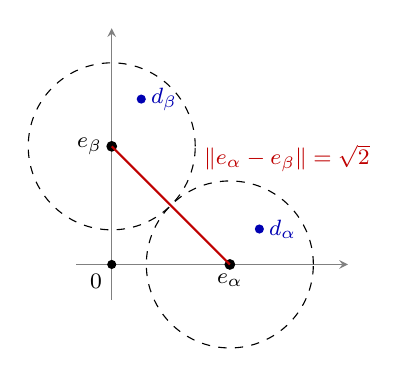
\begin{tikzpicture}[scale=1.5, >=stealth]
    \draw[->, thin, gray] (-0.3,0) -- (2.0,0);
    \draw[->, thin, gray] (0,-0.3) -- (0,2.0);
    \draw[dashed] (1,0) circle (0.707);
    \draw[dashed] (0,1) circle (0.707);
    \fill (1,0) circle (1.3pt) node[below, font=\footnotesize] {$e_\alpha$};
    \fill (0,1) circle (1.3pt) node[left, font=\footnotesize] {$e_\beta$};
    \draw[red!75!black, thick] (1,0) -- (0,1);
    \node[anchor=south west, font=\footnotesize, red!75!black] at (0.7,0.7) {$\|e_\alpha - e_\beta\| = \sqrt{2}$};
    \fill[blue!70!black] (1.25,0.3) circle (1.1pt) node[right, font=\footnotesize] {$d_\alpha$};
    \fill[blue!70!black] (0.25,1.4) circle (1.1pt) node[right, font=\footnotesize] {$d_\beta$};
    \fill (0,0) circle (1.1pt) node[below left, font=\footnotesize] {$0$};
\end{tikzpicture}
\end{center}
Orthonormal vectors are all at distance $\sqrt{2}$ from one another, so balls of radius $\sqrt{2}/2$ around them are disjoint, and each must catch its own point of the dense set. The same argument shows that $L^\infty$ is not separable (MATH 551 notes, Chapter \emph{$L^p$ Spaces}, subsection \emph{Density and Separability}).

\begin{thmbox}[{{$L^2(\mathbb{R}^n)$ is Separable}}]\boxlabel{thm:L2-separable}
$L^2(\mathbb{R}^n)$ is separable, and every orthonormal basis of it is countably infinite.
\end{thmbox}

\begin{proof}
Separability is now also the case $p = 2$, $E = \mathbb{R}^n$ of Proposition~\ref{prop:Lp-separable} (Lecture 9). It is proved in the MATH 551 notes (Chapter \emph{$L^p$ Spaces}, subsection \emph{Density and Separability}): finite linear combinations of indicator functions of boxes with rational endpoints, with rational coefficients (with coefficients in $\mathbb{Q} + i\mathbb{Q}$ in the complex case), form a countable dense set. By Proposition~\ref{prop:sep-countable} every orthonormal basis is countable. It is not finite: the normalized indicators of disjoint unit cubes form an infinite orthonormal set, and a finite orthonormal basis $\{e_1, \ldots, e_N\}$ would make every $x$ a finite combination $\sum_{j \le N} (x, e_j) e_j$, so $L^2(\mathbb{R}^n)$ would have dimension at most $N$ and could not contain $N+1$ orthonormal (hence linearly independent) vectors.
\end{proof}

\begin{rembox}[There is No Dimension Mismatch]\label{rem:no-dimension-mismatch}
The \emph{Hilbert dimension} of $H$ is the cardinality of an orthonormal basis; in $L^2(\mathbb{R}^n)$ it is countable, and by the theorem every orthonormal set, let alone basis, in $L^2(\mathbb{R}^n)$ is countable. So the uncountable family $\{|x\rangle\}$ cannot be an orthonormal set of $L^2$ --- and indeed its elements are not in $L^2$ at all, as the next two propositions show. The correct comparison is not ``countable basis versus uncountable basis'' but ``orthonormal basis versus a different kind of object.''
\end{rembox}

\subsection{Position Has No Eigenvectors}

\begin{propbox}[Position Has No Eigenvectors]\boxlabel{prop:no-eigen}
Let $\psi \in L^2(\mathbb{R})$ and $\lambda \in \mathbb{R}$ satisfy $x\,\psi(x) = \lambda\,\psi(x)$ for almost every $x$. Then $\psi = 0$ in $L^2$.
\end{propbox}

\begin{proof}
$(x - \lambda)\psi(x) = 0$ for almost every $x$, so $\psi(x) = 0$ for almost every $x \neq \lambda$. Since $\{\lambda\}$ has measure zero, $\psi = 0$ almost everywhere.
\end{proof}

\begin{propbox}[Point Evaluation is Not Bounded]\boxlabel{prop:delta}
Let $x_0 \in \mathbb{R}$. There is no $\psi \in L^2(\mathbb{R})$ with
\[
(\varphi, \psi) = \varphi(x_0) \qquad \text{for all } \varphi \in C_c(\mathbb{R}) .
\]
\end{propbox}

\begin{proof}
Suppose such $\psi$ exists. By Cauchy--Schwarz, $|\varphi(x_0)| = |(\varphi, \psi)| \le \|\psi\|_2\,\|\varphi\|_2$ for all $\varphi \in C_c(\mathbb{R})$. Let $\varphi_n$ be the tent function with $\varphi_n(x_0) = 1$, vanishing outside $[x_0 - \frac1n, x_0 + \frac1n]$ and linear in between. Then $0 \le \varphi_n \le 1$, so $\|\varphi_n\|_2^2 \le \frac{2}{n}$, and $1 = |\varphi_n(x_0)| \le \|\psi\|_2 \sqrt{2/n} \to 0$, a contradiction.
\end{proof}

\begin{rembox}[What $|x_0\rangle$ Would Have to Be]\label{rem:what-x0-would-have}
In Dirac notation a position eigenstate is characterized by $\langle x_0 | \varphi \rangle = \varphi(x_0)$, i.e.\ $(\varphi, |x_0\rangle) = \varphi(x_0)$. Proposition~\ref{prop:delta} says no element of $L^2$ does this: the functional $\varphi \mapsto \varphi(x_0)$ is unbounded in the $L^2$ norm, so by the Riesz theorem it is not a bra, and $|x_0\rangle$ is not a ket. (Point evaluation is not even well defined on $L^2$, whose elements are functions up to sets of measure zero.) The ``wavefunction'' of $|x_0\rangle$ would be $\delta(x - x_0)$, and the physicists' normalization $\langle x | x' \rangle = \delta(x - x')$ in place of $1$ is the symptom. Proposition~\ref{prop:no-eigen} says the same thing from the operator side: multiplication by $x$ has no eigenvalues at all.
\end{rembox}

\subsection{The Position Resolution of the Identity}

The object that does exist is the family of projections ``$\int_B |x\rangle\langle x|\,dx$'', one for each region $B$.

\begin{propbox}[The Spectral Projections of Position]\boxlabel{prop:pvm}
For a measurable set $B \subset \mathbb{R}^n$ define $E(B) : L^2(\mathbb{R}^n) \to L^2(\mathbb{R}^n)$ by $E(B)\psi = \chi_B\,\psi$. Then:
\begin{enumerate}[label=(\alph*)]
    \item $E(B)$ is the orthogonal projection onto the closed subspace $\{ \psi : \psi = 0 \text{ a.e.\ outside } B \}$;
    \item $E(\varnothing) = 0$ and $E(\mathbb{R}^n) = \Id$;
    \item if $B_1, B_2, \ldots$ are pairwise disjoint with union $B$, then $\sum_k E(B_k) = E(B)$ strongly;
    \item $(E(B)\psi, \psi) = \int_B |\psi(x)|^2\,dx$.
\end{enumerate}
\end{propbox}

\begin{proof}
Let $Y_B = \{ \psi : \psi = 0 \text{ a.e.\ outside } B \}$, a linear subspace. It is closed: an $L^2$-convergent sequence has an a.e.\ convergent subsequence (MATH 551 notes, Riesz--Fischer), so a limit of functions vanishing a.e.\ outside $B$ vanishes a.e.\ outside $B$. Its orthogonal complement contains every $\phi$ vanishing a.e.\ on $B$, since then $(\psi, \phi) = \int \psi\bar{\phi} = 0$ for $\psi \in Y_B$. Now $\psi = \chi_B\psi + \chi_{B^c}\psi$ with $\chi_B\psi \in Y_B$ and $\chi_{B^c}\psi \in Y_B^\perp$, so by uniqueness in Theorem~\ref{thm:orth-decomp}, $P_{Y_B}\psi = \chi_B\psi$, proving (a). (b) is clear. For (c), $\sum_{k \le N} E(B_k)\psi = \chi_{B_1 \cup \cdots \cup B_N}\psi$, and
\[
\Bigl\| E(B)\psi - \sum_{k \le N} E(B_k)\psi \Bigr\|^2 = \int_{\bigcup_{k > N} B_k} |\psi|^2 \to 0
\]
by the dominated convergence theorem (the integrand $\chi_{\bigcup_{k>N}B_k}|\psi|^2$ tends to $0$ pointwise and is dominated by $|\psi|^2$). (d) $(\chi_B\psi, \psi) = \int \chi_B |\psi|^2$.
\end{proof}

\begin{center}
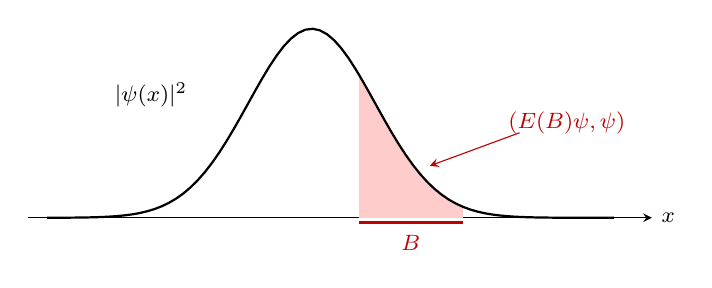
\begin{tikzpicture}[scale=1.2, >=stealth]
    \draw[->] (-3.2,0) -- (3.4,0) node[right, font=\footnotesize] {$x$};
    \fill[red!20, domain=0.3:1.4, samples=40] (0.3,0) -- plot (\x, {2*exp(-(\x+0.2)*(\x+0.2)/0.9)}) -- (1.4,0) -- cycle;
    \draw[thick, domain=-3:3, samples=80] plot (\x, {2*exp(-(\x+0.2)*(\x+0.2)/0.9)});
    \node[font=\footnotesize] at (-1.9,1.3) {$|\psi(x)|^2$};
    \draw[thick, red!75!black] (0.3,-0.05) -- (1.4,-0.05);
    \node[below, font=\footnotesize, red!75!black] at (0.85,-0.08) {$B$};
    \node[font=\footnotesize, red!75!black] at (2.5,1.0) {$(E(B)\psi, \psi)$};
    \draw[->, thin, red!75!black] (2.0,0.9) -- (1.05,0.55);
\end{tikzpicture}
\end{center}

\begin{rembox}[{{Reading $\int |x\rangle\langle x|\,dx = \Id$}}]\label{rem:reading-xgen-x-dx}
The proposition is the rigorous form of the continuous completeness relation. The symbol $\int_B |x\rangle\langle x|\,dx$ means $E(B)$, a genuine bounded operator even though no $|x\rangle$ is a vector; (b) is ``$\int_{\mathbb{R}^n} |x\rangle\langle x|\,dx = \Id$''; (c) replaces ``summing over basis states'' by countable additivity over disjoint regions, again in the strong sense; and (d) is the Born rule --- the probability of finding the particle in $B$. A map $B \mapsto E(B)$ with these properties is a \emph{projection-valued measure}. The spectral theorem, later in the course, will attach one to every self-adjoint operator: for an operator with a basis of eigenvectors it is $E(B) = \sum_{\lambda_n \in B} |e_n\rangle\langle e_n|$, for position it is the one above, and in general it mixes both. The kets $|x\rangle$ themselves can be given a rigorous meaning as elements of a larger space of distributions, via a rigged Hilbert space $\mathcal{S} \subset L^2 \subset \mathcal{S}'$; that construction is not needed for anything above.
\end{rembox}

\begin{rembox}[How the Discrete and Continuous Relations Fit Together]\label{rem:how-discrete-continuous-relations-fit-together}
If $\{e_n\}$ is an orthonormal basis of $L^2(\mathbb{R}^n)$, physics writes $\sum_n e_n(x)\,\overline{e_n(x')} = \delta(x - x')$. Taken literally the left side need not converge anywhere. Integrated against $\varphi(x)$ and $\overline{\chi(x')}$ with $\varphi, \chi \in L^2$, it becomes $\sum_n (\varphi, e_n)(e_n, \chi) = (\varphi, \chi)$, which is Corollary~\ref{cor:insert}. So the distributional identity is exactly ``inserting a complete set of states'', and countably many $L^2$ functions can ``sum to a delta'' because the delta is not in $L^2$.
\end{rembox}

% ============================================================================
% SECTION 25: DISCRETE AND CONTINUOUS SPECTRUM: HYDROGEN
% ============================================================================

\section{Bound States Need Not Be Complete: Hydrogen}\label{sec:qm-hydrogen}

\roadmark{Companion}{Thread: dimension. Discrete and continuous spectrum.}

\begin{thmbox}[Spectrum of the Hydrogen Atom]\boxlabel{thm:hydrogen}
In atomic units, the hydrogen Hamiltonian $H_{\mathrm{hyd}} = -\tfrac12 \Delta - \tfrac{1}{|x|}$ on $L^2(\mathbb{R}^3)$ (spin ignored) is self-adjoint. Its eigenvalues are $E_n = -\tfrac{1}{2n^2}$, $n = 1, 2, \ldots$, with eigenspaces of dimension $n^2$, and its spectrum also contains the continuum $[0, \infty)$, which carries no eigenvectors. In particular the closed linear span $Y_{\mathrm{b}}$ of all eigenfunctions (the bound states) is a proper subspace of $L^2(\mathbb{R}^3)$.
\end{thmbox}

\begin{proof}
Not covered, and beyond the course: it requires the theory of unbounded self-adjoint operators. Recorded here as physics input; see for instance G.~Teschl, \emph{Mathematical Methods in Quantum Mechanics}, the chapter on the hydrogen atom.
\end{proof}

\begin{corbox}[Bound States are Not Complete]\boxlabel{cor:hydrogen-incomplete}
Let $\{\psi_{nlm}\}$ be an orthonormal basis of eigenfunctions of $Y_{\mathrm{b}}$. Then $\{\psi_{nlm}\}$ is not a complete orthonormal set in $L^2(\mathbb{R}^3)$, and there are states $\psi$ with
\[
\sum_{n,l,m} |(\psi, \psi_{nlm})|^2 < \|\psi\|^2 .
\]
\end{corbox}

\begin{proof}
$Y_{\mathrm{b}}$ is a closed proper subspace, so by Theorem~\ref{thm:orth-decomp} its orthogonal complement is nonzero; any $0 \neq \psi \in Y_{\mathrm{b}}^\perp$ is orthogonal to every $\psi_{nlm}$, so the set is not complete. By Theorem~\ref{thm:onbasis-equiv} it is then not an orthonormal basis and Parseval's equality fails for some $\psi$; with Bessel's inequality (Theorem~\ref{thm:bessel}) the inequality is strict for that $\psi$.
\end{proof}

\begin{rembox}[Physical Reading]\label{rem:physical-reading}
For a normalized state $\psi$, $\sum_{n,l,m} |(\psi, \psi_{nlm})|^2$ is the probability of finding the electron in \emph{some} bound state, and Bessel's inequality says it is at most $1$. The deficit $1 - \sum |(\psi, \psi_{nlm})|^2 = \|P_{Y_{\mathrm{b}}^\perp}\psi\|^2$ is the ionization probability. The completeness relation for hydrogen must therefore include the scattering states,
\[
\sum_{n,l,m} |nlm\rangle\langle nlm| + \int_0^\infty dE\, \sum_{l,m} |E\,l\,m\rangle\langle E\,l\,m| = \Id,
\]
where, as with $|x\rangle$, the continuum ``states'' are not in $L^2$ and the integral stands for a projection-valued measure on $[0,\infty)$. By contrast, a system confined to a compact region (the ring of the example in \ref{sec:qm-completeness}, a particle in a box) or by a potential growing at infinity (the harmonic oscillator) has purely discrete spectrum, and its eigenstates alone form an orthonormal basis --- as the ring example shows, compactness forces discreteness. Hydrogen's potential decays at infinity, which is what lets the electron escape and creates the continuum.
\end{rembox}

\begin{rembox}[To Be Continued]\label{rem:continued}
Planned additions as the course proceeds: bounded operators and their adjoints (observables and the dagger, $\langle y | A x \rangle = \langle A^\dagger y | x \rangle$); self-adjoint and unitary operators (observables and time evolution); compact self-adjoint operators and the spectral theorem (the rigorous version of ``diagonalize the Hamiltonian''); and the precise relation between the spectrum of an operator and the measurement outcomes of the corresponding observable.
\end{rembox}

% ============================================================================
% PROBLEM-SOLVING TECHNIQUES
% ============================================================================

\chapter{Problem-Solving Techniques}

This appendix distills the recurring proof strategies from homework problems in the course. It is organized by technique rather than by topic.

% Own numbering for the appendix: headings unnumbered, examples T1, T2, ...
\setcounter{subsection}{0}
\renewcommand{\thesubsection}{}
\titleformat{\subsection}{\large\bfseries}{}{0em}{}
\renewcommand{\exboxnum}{T\arabic{subsection}}

% --------------------------------------------------------------------------
\subsection{Technique 1: Well-Definedness on Quotients}

Any operation on $X/Y$ defined through representatives must be shown independent of the representative before anything else is proved.

\begin{rembox}[Strategy]\label{rem:tech1}
To show $[x] \mapsto F(x)$ is well defined on $X/Y$: take $[x] = [x']$, i.e.\ $x - x' \in Y$, and show $F(x) = F(x')$. For operations built from those of $X$, the difference of the two candidate outputs is a linear combination of elements of $Y$, hence in $Y$ by closure. Only after this do the axioms or other properties get checked, and then each follows by ``definition $\to$ axiom of $X$ $\to$ definition.''
\end{rembox}

\begin{exbox}[Applications (HW1)]\boxlabel{ex:tech1}
\begin{itemize}
\item \textbf{$X/Y$ is a linear space}: $[x_1]+[x_2] := [x_1+x_2]$ and $a[x] := [ax]$ are well defined because $(x_1+x_2)-(x_1'+x_2') = (x_1-x_1')+(x_2-x_2') \in Y$ and $ax - ax' = a(x-x') \in Y$; each axiom then transfers from $X$ in one line.
\item \textbf{Surjectivity of $X \to X/Y \oplus Y$}: to hit $([x], y)$, replace $x$ by the representative $w$ of its class lying in the complement $W$; $[w] = [x]$ since $x - w \in Y$.
\end{itemize}
\end{exbox}

% --------------------------------------------------------------------------
\subsection{Technique 2: Trivial Intersection Gives Uniqueness}

\begin{rembox}[Strategy]\label{rem:tech2}
To show a representation $x = w + y$ ($w \in W$, $y \in Y$) is unique, or that a map reading off components is injective: subtract two representations. The difference $w_1 - w_2 = y_2 - y_1$ lies in $W \cap Y$; if that is $\{0\}$, both differences vanish. The same argument shows $[w_1] = [w_2]$ in $X/Y$ forces $w_1 = w_2$ for $w_i \in W$.
\end{rembox}

\begin{exbox}[Applications (HW1)]\boxlabel{ex:tech2}
\begin{itemize}
\item \textbf{Unique decomposition} for a complement $W$ of $Y$ (Lemma~\ref{lem:unique-decomp}).
\item \textbf{Injectivity of $M : X \to X/Y \oplus Y$} and of $W \to X/Y$, $w \mapsto [w]$ (Theorem~\ref{thm:quotient-iso}, Corollary~\ref{cor:complement-quotient}).
\end{itemize}
\end{exbox}

% --------------------------------------------------------------------------
\subsection{Technique 3: One-Step Enlargement plus Zorn}

The pattern of the Hahn--Banach proof, reusable whenever a maximal object with a closure property is needed.

\begin{rembox}[Strategy]\label{rem:tech3}
\begin{enumerate}[label=(\roman*)]
\item \textbf{One-step lemma}: show that if the desired property holds for an object $W$ and $W$ is not yet ``full,'' there is a strictly larger $W'$ with the same property. This is where the actual mathematics lives.
\item \textbf{Poset}: let $P$ be the set of all objects with the property, ordered by inclusion/extension. Check $P \neq \varnothing$ and that chains have upper bounds --- usually the union of the chain, with the property inherited because it holds member-by-member and any finitely many elements of the union lie in a single member.
\item \textbf{Maximal element}: Zorn gives one; the one-step lemma shows it must be full.
\end{enumerate}
In finite dimensions replace (ii)--(iii) by iterating (i) finitely many times.
\end{rembox}

\begin{exbox}[Applications]\boxlabel{ex:tech3}
\begin{itemize}
\item \textbf{Hahn--Banach} (lecture): objects are pairs $(Z, \ell_Z)$ with $\ell_Z \le p$; one-step lemma is Lemma~\ref{lem:one-step}.
\item \textbf{Existence of a complement} (HW1): objects are subspaces $W$ with $W \cap Y = \{0\}$; one-step lemma is Lemma~\ref{lem:enlarge}.
\item \textbf{Existence of an orthonormal basis} (Lecture 9, Theorem~\ref{thm:onbasis-exists}): objects are orthonormal sets; the one-step move adds $x/\|x\|$ for a nonzero $x$ orthogonal to all of them.
\end{itemize}
\end{exbox}

% --------------------------------------------------------------------------
\subsection{Technique 4: Linearity via Uniqueness}

\begin{rembox}[Strategy]\label{rem:tech4}
When a map is defined by ``decompose $x$ and read off a component,'' prove linearity by decomposing $a x_1 + b x_2$ \emph{by hand} as $(a w_1 + b w_2) + (a y_1 + b y_2)$, checking each summand lies in the right subspace by closure, and invoking uniqueness of the decomposition to conclude that this is the decomposition the map sees.
\end{rembox}

\begin{exbox}[Application (HW1)]\boxlabel{ex:tech4}
Linearity of $M(x) = ([w], y)$ in Theorem~\ref{thm:quotient-iso}. The same device proves linearity of any projection onto a summand of a direct sum.
\end{exbox}


% --------------------------------------------------------------------------
\subsection{Technique 5: Completeness --- Find the Candidate, Then Close}

\begin{rembox}[Strategy]\label{rem:tech5}
To prove a normed space is complete, take a Cauchy sequence and proceed in two separate stages, never merged.
\begin{enumerate}[label=(\roman*)]
\item \textbf{Candidate.} Use the Cauchy property in a \emph{weaker} form that reduces to a space already known complete --- coordinatewise for sequence spaces ($\mathbb{F}$ is complete), pointwise or almost everywhere for function spaces (via a subsequence) --- and let that produce an object $a$. At this stage nothing is known about $a$ except that it exists.
\item \textbf{Closing.} Return to the Cauchy property in its \emph{full} form, with the $N$ fixed once and for all, and show both that $a$ lies in the space and that $\|a^{(n)} - a\| \to 0$. The second usually gives the first: $a = a^{(N)} + (a - a^{(N)})$.
\end{enumerate}
Wu: ``In any completeness problem, the first thing you need to do is find the candidate. Then try to argue the sequence does converge. If you don't have a candidate, we have nothing to do.''
\end{rembox}

\begin{exbox}[Applications]\boxlabel{ex:tech5}
\begin{itemize}
\item \textbf{$\ell^p$ complete} (lecture, Theorem~\ref{thm:lp-complete}): candidate by coordinates; closing by the tail estimate \eqref{eq:lp-tail}.
\item \textbf{Completion of a normed space} (HW2 P3, Theorem~\ref{thm:completion-normed}): candidate is the diagonal sequence $y_j = x^{(M_j)}_{N_j}$; closing by two three-term triangle inequalities with an auxiliary index sent to infinity last.
\item \textbf{$C[a,b]$ with the sup norm} (HW2 P1, Theorem~\ref{thm:Cab-banach}): candidate by pointwise limits; closing by uniform convergence, then the $3\varepsilon$ argument for continuity of the limit.
\end{itemize}
\end{exbox}

% --------------------------------------------------------------------------
\subsection{Technique 6: Truncate, Then Pass to the Limit}

\begin{rembox}[Strategy]\label{rem:tech6}
When an estimate involves an infinite sum or an integral that might be infinite, or when two limits interact, cut off to a finite sum first.
\begin{enumerate}[label=(\roman*)]
\item Prove the inequality for finitely supported objects, where every quantity is finite and algebra (dividing, cancelling) is legitimate.
\item Apply it to the truncations $a^{(n)} = (a_1, \ldots, a_n, 0, \ldots)$, bound the right side by the untruncated quantity (a partial sum of non-negative terms is at most the full sum), and let $n \to \infty$ using monotone convergence of the partial sums.
\end{enumerate}
When two limits are present (an index $m \to \infty$ inside a sum over $i$, and the length $k$ of the sum $\to \infty$): keep the full-strength hypothesis with its uniform $N$, truncate to $k$ terms, pass $m \to \infty$ termwise through the finite sum, and only then send $k \to \infty$. Never let the threshold $N$ depend on $k$.
\end{rembox}

\begin{exbox}[Applications]\boxlabel{ex:tech6}
\begin{itemize}
\item \textbf{Minkowski for sequences} (lecture, Theorem~\ref{thm:minkowski-seq}): the cancellation of $\|a+b\|_p^{\,p-1}$ is only valid for finitely supported sequences; the general case follows by truncation.
\item \textbf{Completeness of $\ell^p$}, Step 2 (Theorem~\ref{thm:lp-complete}): the order truncate $\to$ $m \to \infty$ $\to$ $k \to \infty$.
\item \textbf{H\"older for finite sums} is the special case of Theorem~\ref{thm:holder-seq} with zero tails; conversely no truncation is needed there because every quantity is a sum of non-negative terms and inequalities in $[0,\infty]$ suffice.
\end{itemize}
\end{exbox}


% --------------------------------------------------------------------------
\subsection{Technique 7: Compactness of the Unit Sphere in Finite Dimensions}

\begin{rembox}[Strategy]\label{rem:tech7}
To get a lower bound $\|x\|' \ge c\|x\|$ between two norms on a finite-dimensional space, or more generally to show a continuous positive function is bounded away from $0$: restrict to the unit sphere $S$ of one norm, show $S$ is sequentially compact (bounded coordinates $\Rightarrow$ Bolzano--Weierstrass coordinate by coordinate), show the function is continuous on $S$ (usually via a one-sided estimate and the reverse triangle inequality), conclude it attains its infimum, and use positivity at the minimizer to get $c > 0$. Homogeneity then extends the bound from $S$ to all of $X$. The step that fails in infinite dimensions is the compactness of $S$.
\end{rembox}

\begin{exbox}[Applications (HW2)]\boxlabel{ex:tech7}
\begin{itemize}
\item \textbf{All norms on $\mathbb{F}^n$ are equivalent} (P2(a), Theorem~\ref{prop:norms-equiv}), Steps 4--7.
\item \textbf{Finite-dimensional subspaces are closed} (P2(b), Corollary~\ref{cor:findim-closed}), via the equivalence with the coordinate norm.
\end{itemize}
\end{exbox}


% --------------------------------------------------------------------------
\subsection{Technique 8: Rotate to Make it Real}

\begin{rembox}[Strategy]\label{rem:tech8}
A real inequality of the form $\operatorname{Re}\Lambda(x) \le p(x)$ gives no control on $|\Lambda(x)|$ directly. To upgrade it, multiply $x$ by a unimodular scalar chosen for that one $x$: write $\Lambda(x) = |\Lambda(x)|e^{i\varphi}$ and set $a = e^{-i\varphi}$, so that $\Lambda(ax) = a\Lambda(x) = |\Lambda(x)|$ is real and non-negative, hence equals its own real part. Applying the real bound to $ax$ and using $|a| = 1$ to undo the rotation on the right gives $|\Lambda(x)| \le p(x)$ with constant $1$. The gain over splitting into real and imaginary parts is the constant: that route costs a factor $\sqrt{2}$, because it uses the bound twice.
\end{rembox}

\begin{exbox}[Applications]\boxlabel{ex:tech8}
\begin{itemize}
\item \textbf{Complex Hahn--Banach}, Step 5 (Theorem~\ref{thm:hb-complex}): rotate $x$ so that $L(ax)$ is real, then apply $U \le p$.
\item \textbf{Cauchy--Schwarz}, Step 4 (Theorem~\ref{thm:cauchy-schwarz}): rotate $y$ so that $(e^{i\theta}y, x)$ is real, then apply the bound on $|\operatorname{Re}(y,x)|$ obtained from the real quadratic.
\end{itemize}
\end{exbox}


% --------------------------------------------------------------------------
\subsection{Technique 9: Incompleteness and Identifying the Completion}

\begin{rembox}[Strategy]\label{rem:tech9}
To show a normed space $(X, \|\cdot\|)$ is not complete and find its completion:
\begin{enumerate}[label=(\roman*)]
\item find a Banach space $Z$ and a norm-preserving linear map $J : X \to Z$ (often an inclusion, or $f \mapsto [f]$ into an $L^p$ space);
\item show $J(X)$ is dense in $Z$;
\item show $J(X) \ne Z$ by exhibiting $z \in Z \setminus J(X)$.
\end{enumerate}
Then $\overline{X} = Z$ (Proposition~\ref{prop:identify-completion}), and $X$ is not complete, because a sequence in $X$ whose image converges to $z$ is Cauchy with no limit in $X$. When a proof without the ambient $Z$ is wanted, write the Cauchy sequence down explicitly and show that any limit in $X$ would have to violate the defining property of $X$ (continuity, differentiability, \ldots). Before starting, check the norm, not only the set: the same set may be complete under one norm and not under another.
\end{rembox}

\begin{exbox}[Applications (HW3)]\boxlabel{ex:tech9}
\begin{itemize}
\item \textbf{$C[a,b]$ in the $L^p$ norm} (P1, Proposition~\ref{prop:completion-L1}): $Z = L^p[a,b]$; witness the step function, approached by ramps.
\item \textbf{$C^2[a,b]$ in the norm $\max|f| + \max|f'|$} (P2, Proposition~\ref{prop:C2-incomplete}): $Z = C^1[a,b]$; density by approximating $f'$ uniformly and integrating; witness $|x - c|^{3/2}$.
\item \textbf{Contrast}: $C[a,b]$ in the sup norm is already complete (Theorem~\ref{thm:Cab-banach}), and so is $C^2[a,b]$ in the full $C^2$ norm.
\end{itemize}
\end{exbox}

% --------------------------------------------------------------------------
\subsection{Technique 10: From $\mathbb{N}$ to $\mathbb{R}$ by Continuity}

\begin{rembox}[Strategy]\label{rem:tech10}
To prove $F(ax) = aF(x)$ for all real $a$ from additivity $F(x + y) = F(x) + F(y)$: induction gives $a \in \mathbb{N}$; $F(0) = 0$ and $F(-x) = -F(x)$ give $a \in \mathbb{Z}$; $n F(\frac{m}{n}x) = F(mx) = mF(x)$ gives $a \in \mathbb{Q}$; and continuity of $a \mapsto F(ax)$, together with density of $\mathbb{Q}$, gives $a \in \mathbb{R}$. The last step is the only analytic one and cannot be skipped.
\end{rembox}

\begin{exbox}[Application (HW3)]\boxlabel{ex:tech10}
Real homogeneity of the polarization form in the Jordan--von Neumann theorem (P3, Theorem~\ref{thm:jvn}), with continuity supplied by continuity of the norm.
\end{exbox}


% --------------------------------------------------------------------------
\subsection{Technique 11: Minimize, Then Perturb}

\begin{rembox}[Strategy]\label{rem:tech11}
To produce a point with a geometric property (closest point, orthogonal vector) in a Hilbert space:
\begin{enumerate}[label=(\roman*)]
\item \textbf{Minimize.} Take a minimizing sequence for the relevant infimum, and show it is Cauchy by applying the parallelogram law to two of its terms; convexity of the constraint set puts the midpoint back in the set and makes the cross term large. Completeness gives a limit; closedness keeps it in the set.
\item \textbf{Perturb.} To extract the property of the minimizer, compare it with nearby competitors $y_0 + ty$, expand $\|v - ty\|^2$, and let $t \to 0$ along a ray $t = s e^{i\theta}$ chosen (Technique~8) to make the linear term real: a minimum forces the coefficient of the linear term to vanish. Write down explicitly how small $s$ must be.
\end{enumerate}
The same two moves prove uniqueness (apply (i) to two minimizers) and the double-complement identity (apply (ii) to the decomposition).
\end{rembox}

\begin{exbox}[Applications]\boxlabel{ex:tech11}
\begin{itemize}
\item \textbf{Projection theorem} (Theorem~\ref{thm:projection}): step (i).
\item \textbf{Orthogonal decomposition} (Theorem~\ref{thm:orth-decomp}): step (i) applied to $K = Y$, then step (ii) to show $x_0 - y_0 \perp Y$.
\item \textbf{Cauchy--Schwarz} (Theorem~\ref{thm:cauchy-schwarz}) is step (ii) in disguise: $\|x + ty\|^2 \ge 0$ for all $t$, with the quadratic in $t$ minimized at $t = -B/A$.
\end{itemize}
\end{exbox}


% --------------------------------------------------------------------------
\subsection{Technique 12: Countability by Level Sets}

\begin{rembox}[Strategy]\label{rem:tech12}
To show that $S = \{ \alpha : t_\alpha \neq 0 \}$ is countable for a family of numbers $(t_\alpha)$ over a possibly uncountable index set, split it into level sets $\Lambda_k = \{ \alpha : |t_\alpha| \ge 1/k \}$, so that $S = \bigcup_k \Lambda_k$, and bound the number of elements of each $\Lambda_k$ by an inequality that holds for every \emph{finite} subset, such as a finite Bessel inequality or a finite measure bound. Wu: ``you want to show something is finite, and then you take a lower bound.'' Only finite subsets can be fed into the inequality; the uniform bound on them is what proves $\Lambda_k$ finite.
\end{rembox}

\begin{exbox}[Application]\boxlabel{ex:tech12}
Countable support of the orthonormal coefficients $(x, e_\alpha)$ (Proposition~\ref{prop:countable-support}), with $\#\Lambda_k \le k^2\|x\|^2$ from Lemma~\ref{lem:finite-bessel}.
\end{exbox}


% --------------------------------------------------------------------------
\subsection{Technique 13: Test Against a Well-Chosen Vector}

\begin{rembox}[Strategy]\label{rem:tech13}
To bound $\|h\|$ from below, find a vector $g$ whose inner product with $h$ is determined by the data, and apply Cauchy--Schwarz: $|(h, g)| \le \|h\|\,\|g\|$. The best $g$ lies in the span of the vectors whose inner products with $h$ are prescribed (projection onto that span). Dually, to show a vector is small, bound each of its coefficients by Cauchy--Schwarz and add them up with Parseval.
\end{rembox}

\begin{exbox}[Applications (HW4)]\boxlabel{ex:tech13}
\begin{itemize}
\item \textbf{Sharp integral inequality} (P4, Proposition~\ref{prop:sharp-integral}): $h = f''$, $g$ linear, $(h,g) = -1$ from the boundary data.
\item \textbf{Perturbed orthonormal sets} (P3, Proposition~\ref{prop:perturb-onb}): $(x, e_n) = (x, e_n - f_n)$, then Parseval.
\end{itemize}
\end{exbox}

% --------------------------------------------------------------------------
\subsection{Technique 14: Computing an Orthogonal Complement}

\begin{rembox}[Strategy]\label{rem:tech14}
To show $S^\perp = C$: first guess $C$ and check $C \subset S^\perp$ directly (often by a symmetry). For $S^\perp \subset C$, decompose an arbitrary $g \in S^\perp$ as $g = s + c$ with $s \in S$, $c \in C$, and test $g$ against its own $S$-component: $0 = (g, s) = \|s\|^2 + (c, s) = \|s\|^2$. For a set $M$ that is not a closed subspace, first replace it by $\overline{\operatorname{span}}\, M$, which has the same complement.
\end{rembox}

\begin{exbox}[Applications (HW4)]\boxlabel{ex:tech14}
\begin{itemize}
\item \textbf{Even and odd functions} (P1, Proposition~\ref{prop:even-odd}): symmetry gives $O \subset E^\perp$; testing against $g_e$ gives the rest.
\item \textbf{Double complement} (P2, Theorem~\ref{thm:double-perp}): Lemma~\ref{lem:perp-span}, then Theorem~\ref{thm:orth-decomp}(2).
\end{itemize}
\end{exbox}

% --------------------------------------------------------------------------
\subsection{Technique 15: Separability by Truncation and Rational Approximation}

\begin{rembox}[Strategy]\label{rem:tech15}
To show a space is separable, write down a countable set built from finitely many rational parameters (finitely many rational coordinates, rational coefficients on finitely many basis vectors, rational heights on rational rectangles). Countability: a countable union over the number of parameters of countable products. Density: first cut off a small ``tail'' (the tail of a convergent series or expansion, or the part of a function outside a large box), then replace the finitely many remaining parameters by nearby rationals. The first step is what fails in $\ell^\infty$ and $L^\infty$, where the norm is a supremum rather than a sum or integral.
\end{rembox}

\begin{exbox}[Applications (Lecture 9)]\boxlabel{ex:tech15}
\begin{itemize}
\item $\ell^p$, $1 \le p < \infty$ (Proposition~\ref{prop:lp-separable}).
\item $L^p(E)$, $1 \le p < \infty$ (Proposition~\ref{prop:Lp-separable}), after reducing to continuous functions.
\item A Hilbert space with a countable orthonormal basis (Theorem~\ref{thm:sep-countable-onb}, $\Rightarrow$).
\end{itemize}
\end{exbox}

% ============================================================================
% CONCORDANCE WITH LAX
% ============================================================================

\chapter{Concordance with Lax}

The course follows Lax, \emph{Functional Analysis}, Chapters 1, 3, 5, 6 and 15, but not always by the same route. This chapter records the differences so that the notes and the book can be read side by side: notation (Table~C.1), where the two routes diverge (C.2), which parts of the notes correspond to which parts of the book (C.3), and an index of every Lax result cited in the notes, ordered by Lax's chapter and section (C.4); within a section, items Lax does not number (definitions, displayed conditions) come first in the order the notes use them, followed by numbered results in Lax's numbering. The index is generated by \texttt{qa556.py} from the reference lines at the foot of the boxes, so it cannot drift from the notes.

\section*{C.1 Notation}
\addcontentsline{toc}{section}{C.1 Notation}

{\small
\begin{longtable}{p{3.8cm} p{5.4cm} p{5.6cm}}
\textbf{Object} & \textbf{These notes} & \textbf{Lax} \\ \hline \endhead
Norm & $\|x\|$ (Wu writes $|x|$ on the board) & $|x|$; $\|x\|$ for a norm induced by a scalar product \\
$p$-norm & $\|a\|_p$ & $|x|_p$ \\
Class mod $Y$ & $[x]$; $x - x' \in Y$ & $\{x\}$; $x_1 \equiv x_2 \pmod Y$ \\
Functional and its extension & $\ell$ on $Y$, extended to $L$ on $X$ & $f$ (or $\ell$) for both \\
Positive homogeneity & $p(ax) = a\,p(x)$ for $a \ge 0$ & for $a > 0$ (equivalent; see C.2) \\
Closed unit ball & $\overline{B_1(0)}$ & $B_1$ \\
Compact & sequentially compact; agrees with the open-cover notion (Theorem~\ref{thm:compact-seq}) & ``compact'' in the sequential sense (\S5.2) \\
Scalar product & $(x,y)$, linear in $x$, conjugate-linear in $y$ & the same \\
Riesz representer & $\ell(x) = (x, a)$ & $\ell(x) = (x, y)$ \\
Linear maps & $T : X \to Y$, $\|T\|$, $\mathcal{L}(X, Y)$ & $M : X \to U$, $|M|$, $\mathcal{L}(X, U)$ \\
Orthonormal family & $\{e_\alpha\}_{\alpha \in \Lambda}$, any index set & $\{x_j\}$ \\
Orthonormal basis & defined by the expansion $x = \sum_\alpha (x, e_\alpha) e_\alpha$ & ``orthonormal base'', defined by $\overline{\operatorname{span}} = H$ \\
Complement & complement $W$ of $Y$ (\S\ref{subsec:complements}); $X = Y \oplus W$ & complementary subspaces \\
Sobolev space & $H^k_0(\Omega)$, completion of $C_c^\infty(\Omega)$ & $W^{k,p}$, completion of $C^\infty$ functions with finite norm \\
Separable & countable $D$ with every point a limit of a sequence in $D$ & countable set whose closure is the whole space (the same, by Definition~\ref{def:closure}) \\
\end{longtable}
}

\section*{C.2 Where the Routes Diverge}
\addcontentsline{toc}{section}{C.2 Where the Routes Diverge}

{\small
\begin{longtable}{p{2.6cm} p{4.3cm} p{4.6cm} p{2.4cm}}
\textbf{Topic} & \textbf{These notes (Wu)} & \textbf{Lax} & \textbf{See} \\ \hline \endhead
Positive homogeneity & $a \ge 0$ & $a > 0$; equivalent, since $p(0) = 2p(0)$ & Lemma~\ref{lem:p-zero} \\
Interior points of $\{p < 1\}$ & every point is interior & only $0$ (Thm~3.4(i)); the rest an exercise & Prop.~\ref{prop:open-interior} \\
Separation & a point from a nonempty convex set all of whose points are interior & also one interior point suffices (Cor.~3.5$'$), and two disjoint convex sets (Thm~3.6); not covered & Thm~\ref{thm:separation} \\
H\"older & proved from Young's inequality & cited from Courant & Thm~\ref{thm:holder-seq} \\
Minkowski & split $|a+b|^p$, H\"older twice, truncation & duality formula $|x|_p = \max_{|u|_q = 1}|(x,u)|$ (Thm~5.5) & Thm~\ref{thm:minkowski-seq} \\
Completeness of $\ell^p$ & proved & asserted (examples (a)--(b)) & Thm~\ref{thm:lp-complete} \\
$L^p$ & working definition by Lebesgue integrable functions; equals the completion of $C[a,b]$ & \emph{defined} as the completion of $C_c$ in the $p$-norm (example (f)) & Prop.~\ref{prop:completion-L1} \\
Sobolev spaces & completion of $C_c^\infty(\Omega)$: $H^k_0$ & completion of $C^\infty$ with finite norm: $W^{k,p}$ (example (g)) & Ex.~\ref{ex:sobolev} \\
Closest point & Hilbert spaces, via the parallelogram law & also uniformly convex Banach spaces (Thm~5.8); not covered & Thm~\ref{thm:projection} \\
Riesz representation & explicit decomposition $x = kx_0 + y$ & functionals with the same null space are proportional (Lemma~6.5) & Thm~\ref{thm:riesz-rep} \\
Orthonormal basis & expansion; equivalent to completeness & closed linear span $= H$ & Prop.~\ref{prop:lax-onb} \\
Existence of an orthonormal basis & maximal orthonormal set is complete: add $x/\|x\|$ & maximal set has closed span $H$, via Bessel & Thm~\ref{thm:onbasis-exists} \\
Continuous $\Rightarrow$ bounded & $y_n = x_n/(n\|x_n\|)$: $\|y_n\| = 1/n$, $\|Ty_n\| > 1$ & $|x_n| = 1/\sqrt{n}$, $|Mx_n| > \sqrt{n}$; stated for Banach spaces & Prop.~\ref{prop:cont-bounded} \\
\end{longtable}
}

\section*{C.3 Chapter Map}
\addcontentsline{toc}{section}{C.3 Chapter Map}

{\small
\begin{longtable}{p{4.3cm} p{3.4cm} p{6.6cm}}
\textbf{These notes} & \textbf{Lax} & \textbf{Comments} \\ \hline \endhead
\ref{sec:lin-spaces}--\ref{sec:maps-convex} Linear spaces, maps, convexity & Ch.~1; \S3.1 & Complements and $X \cong X/Y \oplus Y$ (\S\ref{subsec:complements}, HW1) are not in Lax; extreme subsets (Lax Ch.~1) not covered. \\
\ref{sec:hb-statement}--\ref{sec:hb-proof} Hahn--Banach & \S3.1, Thm~1 & Same proof: one-step extension and Zorn. \\
\ref{sec:gauge} Convex sets and the gauge & \S3.1, Thms~2--4 & Notes prove more of the exercises. \\
\ref{sec:separation} Separation & \S3.2, Thm~5 & Strengthenings Cor.~5$'$, Thm~6 not covered. \\
\ref{sec:hb-complex} Complex Hahn--Banach & \S3.3, Thm~8 & Agnew--Morse (Thm~7) not covered. \\
\ref{sec:normed} Normed spaces & \S5.1 & Metric notions (convergence, closure, open sets) spelled out in the notes. \\
\ref{sec:completeness} Completeness & \S5.1, Thm~3; examples (c)--(e) & $C[a,b]$ and the completion proved in full (HW2). \\
\ref{sec:new-from-old} New spaces from old & \S5.1, (5), Thm~1 & Equivalence of norms in finite dimensions (HW2) is not in Lax. \\
\ref{sec:young}--\ref{sec:minkowski} Inequalities, $\ell^p$ & \S5.1, examples (a)--(b), Thms~4--5 & See C.2. \\
\ref{sec:completion-L1-sec} $L^p$ & \S5.1, examples (f)--(g) & See C.2. \\
\ref{sec:noncompact} Compactness & \S5.2, Thm~6, Lemma~7 & Uniform convexity and Mazur--Ulam (\S5.2 and \S5.3) not covered. \\
\ref{sec:inner-def}--\ref{sec:cauchy-schwarz} Inner products & \S6.1 & Jordan--von Neumann is Lax's Exercise~1 (HW3). \\
\ref{sec:projection} Projection & \S6.2, Thms~2--3 & \\
\ref{sec:riesz-rep} Riesz representation & \S6.3, Thm~4 & Lax--Milgram (Thm~6) not covered. \\
\ref{sec:onb} Orthonormal bases & \S6.4; \S5.1 (separability) & Isometries of $H$ (Thm~10) not covered. Separability of $\ell^p$, $L^p$ proved in the notes (Lax asserts). The classification of separable Hilbert spaces is Lax's Exercise~10 (HW5). \\
\ref{sec:bounded-maps} Bounded linear maps & \S15.1, Thms~1--3 & Lax assumes Banach spaces throughout \S15.1; not needed for Thm~1. \\
Chapter~\ref{ch:qm} (companion) & --- & Dual spaces return in Lax Ch.~8. \\
\end{longtable}
}

\section*{C.4 Index of Lax Results Cited}
\addcontentsline{toc}{section}{C.4 Index of Lax Results Cited}

% BEGIN LAX INDEX (generated by qa556.py; do not edit by hand)
{\small
\begin{longtable}{p{4.6cm} p{2.6cm} p{7.1cm}}
\textbf{Lax} & \textbf{Notes} & \textbf{Box} \\ \hline \endhead
Ch.~1, axioms for a linear space & Definition~\ref{def:linear-space} & Linear Space \\
Ch.~1, definition of linear subspace & Definition~\ref{def:linear-subspace} & Linear Subspace \\
Ch.~1, sum of subsets & Definition~\ref{def:sum-of-subsets} & Sum of Subsets \\
Ch.~1, direct sum & Definition~\ref{def:direct-sum} & Direct Sum \\
Ch.~1, definition of linear span & Definition~\ref{def:linear-span} & Linear Span \\
Ch.~1, equivalence mod $Y$ & Definition~\ref{def:equivalence-mod} & Equivalence mod $Y$ \\
Ch.~1, quotient space & Definition~\ref{def:equivalence-class-and-quotient} & Equivalence Class and Quotient Space \\
Ch.~1, quotient space & Proposition~\ref{prop:quotient} & $X/Y$ is a Linear Space \\
Ch.~1, definition of linear map & Definition~\ref{def:linear-map} & Linear Map \\
Ch.~1, definition of isomorphism; Remark~2 & Definition~\ref{def:isomorphism} & Isomorphism \\
Ch.~1, definition of convex set & Definition~\ref{def:convex-set} & Convex Set \\
Ch.~1, definition of convex hull & Definition~\ref{def:convex-hull} & Convex Hull \\
Ch.~1, Thm~1(ii) & Proposition~\ref{prop:sum} & Sum of Subspaces \\
Ch.~1, Thm~2(i) & Proposition~\ref{prop:the-smallest-subspace-exists} & The Smallest Subspace Exists \\
Ch.~1, Thm~2(ii) & Proposition~\ref{prop:span-as-finite-linear} & Span as Finite Linear Combinations \\
Ch.~1, Thm~5(vi) and Thm~6(i) & Proposition~\ref{prop:the-smallest-convex-set} & The Smallest Convex Set Exists \\
\S3.1, definition of linear functional & Definition~\ref{def:linear-functional} & Linear Functional \\
\S3.1, definition of interior point & Definition~\ref{def:interior} & Interior Point \\
\S3.1, equation (8) & Definition~\ref{def:gauge} & Gauge \\
\S3.1, conditions (1)--(2) of Thm~1 & Definition~\ref{def:positive-homogeneous-subadditive} & Positive Homogeneous; Subadditive \\
\S3.1, Thm~1 & Theorem~\ref{thm:hb} & Hahn--Banach \\
\S3.1, proof of Thm~1 & Lemma~\ref{lem:one-step} & One-Step Extension \\
\S3.1, proof of Thm~1 & Theorem~\ref{thm:zorn} & Zorn's Lemma \\
\S3.1, Thm~2 & Proposition~\ref{prop:gauge-sublinear} & The Gauge is Positive Homogeneous and Subadditive \\
\S3.1, Thm~3, (10) & Proposition~\ref{prop:gauge-values} & Values of the Gauge \\
\S3.1, Thm~3, (10$'$) & Proposition~\ref{prop:interior-gauge} & Interior Points of $K$ are Exactly $\{p_K < 1\}$ \\
\S3.1, Thms~3--4 & Corollary~\ref{cor:sublevel} & Convex Sets of Interior Points are Sublevel Sets \\
\S3.1, Thm~4 & Proposition~\ref{prop:sublevel-convex} & Positive Homogeneous Subadditive $p$ Gives a Convex Set \\
\S3.1, Thm~4(i) & Proposition~\ref{prop:open-interior} & Every Point of $\{p < 1\}$ is Interior \\
\S3.2, hyperplanes & Definition~\ref{def:hyperplane} & Hyperplane; Half-Space \\
\S3.2, Thm~5 & Theorem~\ref{thm:separation} & Hyperplane Separation; Geometric Hahn--Banach \\
\S3.3, Thm~8 & Theorem~\ref{thm:hb-complex} & Complex Hahn--Banach \\
\S5.1, (1)--(3) & Definition~\ref{def:norm} & Norm; Normed Linear Space \\
\S5.1, examples (a)--(b), for sequences & Example~\ref{ex:norms-rn} & Norms on $\mathbb{R}^n$ \\
\S5.1, (4) & Proposition~\ref{prop:norm-metric} & A Normed Space is a Metric Space \\
\S5.1, definition of Banach space & Definition~\ref{def:banach-space} & Banach Space \\
\S5.1, examples (c)--(e) & Theorem~\ref{thm:Cab-banach} & $C[a,b]$ with the Supremum Norm is a Banach Space \\
\S5.1, completion of a metric space & Definition~\ref{def:completion} & Completion \\
\S5.1, (5) & Definition~\ref{def:equivalent-norms} & Equivalent Norms \\
\S5.1, construction (i) & Proposition~\ref{prop:subspace-norm} & Subspace Norm \\
\S5.1, (19) & Theorem~\ref{thm:holder-seq} & H\"older's Inequality for Sequences \\
\S5.1, example (b) & Definition~\ref{def:lp} & $\ell^p$ \\
\S5.1, examples (a)--(b) & Theorem~\ref{thm:lp-complete} & $\ell^p$ is a Banach Space \\
\S5.1, example (f) & Definition~\ref{def:Lp} & $L^p(\Omega)$, $L^\infty(\Omega)$ --- working definition \\
\S5.1, example (f) & Proposition~\ref{prop:completion-L1} & $L^p[a,b]$ as a Completion \\
\S5.1, example (g) & Example~\ref{ex:sobolev} & Sobolev Spaces \\
\S5.1, definition of separable space & Definition~\ref{def:separable} & Separable Space \\
\S5.1, construction (ii) and Exercise~1 & Proposition~\ref{prop:direct-sum-norm} & Norms on a Direct Sum \\
\S5.1, Thm~1 & Theorem~\ref{thm:quotient-norm} & Quotient Norm \\
\S5.1, before Thm~2; ``dense'' in the definition of separable space & Definition~\ref{def:closure} & Closure; Dense Subset \\
\S5.1, Thm~2 (part (d)) & Proposition~\ref{prop:closure} & Properties of the Closure \\
\S5.1, Thm~3 & Theorem~\ref{thm:completion-normed} & The Completion of a Normed Space is a Banach Space \\
\S5.1, Thms~4--5 & Theorem~\ref{thm:minkowski-seq} & Minkowski's Inequality for Sequences \\
\S5.1, Thm~4 & Proposition~\ref{prop:lp-normed} & $\ell^p$ is a Normed Linear Space \\
\S5.2, Thm~6 & Theorem~\ref{thm:ball-noncompact} & The Unit Ball of an Infinite-Dimensional Space is Not Compact \\
\S5.2, Lemma~7 & Lemma~\ref{lem:riesz} & Riesz's Lemma \\
\S6.1, (i)--(iii) & Definition~\ref{def:inner-product} & Inner Product; Scalar Product \\
\S6.1, Example~2 & Example~\ref{ex:box} & $\ell^2$ \\
\S6.1, (3) & Theorem~\ref{thm:inner-norm} & The Inner Product Induces a Norm \\
\S6.1, definition of Hilbert space & Definition~\ref{def:hilbert} & Hilbert Space \\
\S6.1, Example~1 & Example~\ref{ex:an-inner-product-space} & An Inner Product Space that is Not a Hilbert Space \\
\S6.1, (6) & Proposition~\ref{prop:parallelogram} & Parallelogram Law and Polarization \\
\S6.1 and \S6.2, definitions & Definition~\ref{def:orth} & Orthogonality; Orthogonal Complement \\
\S6.1, Thm~1 & Theorem~\ref{thm:cauchy-schwarz} & Cauchy--Schwarz \\
\S6.1, Exercise~1 & Theorem~\ref{thm:jvn} & Jordan--von Neumann \\
\S6.1, Exercise~2 & Lemma~\ref{lem:ip-continuous} & The Inner Product is Continuous \\
\S6.2, Thm~2 & Theorem~\ref{thm:projection} & Closest Point in a Closed Convex Set \\
\S6.2, Thm~3(i) & Proposition~\ref{prop:perp-closed} & $M^\perp$ is a Closed Subspace \\
\S6.2, Thm~3 & Theorem~\ref{thm:orth-decomp} & Orthogonal Decomposition \\
\S6.3, (14) & Definition~\ref{def:bounded-functional} & Bounded Linear Functional \\
\S6.3, Thm~4 & Theorem~\ref{thm:riesz-rep} & Riesz Representation Theorem \\
\S6.3, Lemma~5(i) & Lemma~\ref{lem:ker-codim1} & The Kernel Has Codimension One \\
\S6.4, closed linear span & Definition~\ref{def:closed-span} & Closed Linear Span \\
\S6.4, definition of orthonormal set & Definition~\ref{def:onset} & Orthogonal and Orthonormal Sets \\
\S6.4, definition of orthonormal base (via closed linear span; see Proposition~\ref{prop:lax-onb}) & Definition~\ref{def:onbasis} & Orthonormal Basis \\
\S6.4, Thm~7 & Theorem~\ref{thm:double-perp} & The Double Complement \\
\S6.4, definition of orthonormal base and Thm~7 & Proposition~\ref{prop:lax-onb} & Lax's Definition of Orthonormal Base Agrees \\
\S6.4, Lemma~8 & Theorem~\ref{thm:onbasis-equiv} & Characterizations of an Orthonormal Basis \\
\S6.4, Thm~9 & Theorem~\ref{thm:onbasis-exists} & Existence of Orthonormal Bases \\
\S6.4, Thm~9$'$ & Theorem~\ref{thm:sep-countable-onb} & Separable Hilbert Spaces and Countable Bases \\
\S6.4, Thm~9$'$ & Lemma~\ref{lem:gram-schmidt} & Gram--Schmidt \\
\S6.4, Exercise~10 & Theorem~\ref{thm:sep-classification} & Classification of Separable Hilbert Spaces \\
\S15.1, definition of continuous map & Definition~\ref{def:cont-map} & Continuous Linear Map \\
\S15.1, (2) and (2$'$) & Definition~\ref{def:bounded-map} & Bounded Linear Map; Operator Norm \\
\S15.1, (3) and (3$'$) & Proposition~\ref{prop:op-norm} & The Operator Norm \\
\S15.1, definition of $\mathcal{L}(X, U)$ & Definition~\ref{def:LXY} & The Space $\mathcal{L}(X, Y)$ \\
\S15.1, Thm~1 & Proposition~\ref{prop:cont-bounded} & Continuous if and only if Bounded \\
\S15.1, Thms~2--3 & Theorem~\ref{thm:LXY} & $\mathcal{L}(X, Y)$ is a Normed Linear Space \\
\end{longtable}
}
% END LAX INDEX

\end{document}
